\documentclass[10pt]{report}
\usepackage{lmodern}
\usepackage{graphicx}
\usepackage{varwidth}
\usepackage{enumitem}
\usepackage{amsmath}
\usepackage{amssymb}
\usepackage{mathtools}
\usepackage{pifont}
\usepackage{arydshln}
\usepackage{tikz}
\usepackage{lscape}
\usepackage{bm}
\usepackage{nicefrac}
\usepackage{physics}
\usepackage{fontsize}
\usepackage[landscape]{geometry}
\geometry{a4paper, total={296mm,210mm}, left=-5mm, top=0mm}
\renewcommand{\labelenumi}{\bfseries(\alph{enumi})\phantom{x}}
\newcommand\omicron{o}
\hfuzz=50pt
\setlist[enumerate]{leftmargin=0pt,itemindent=34pt}
\pagenumbering{gobble}
\setlength{\tabcolsep}{0pt}
\begin{document}
\thispagestyle{empty}
\begin{tabular}{c:c}
\begin{minipage}[c][104.5mm][t]{0.5\linewidth}
\begin{center}
\vspace{7mm}
{\huge Viazané extrémy, skupina \textit{Alpha $\alpha$} -\romannumeral1}\\[5mm]
\textit{Jméno:}\phantom{xxxxxxxxxxxxxxxxxxxxxxxxxxxxxxxxxxxxxxxxxxxxxxxxxxxxxxxxxxxxxxxxx}\\[5mm]
\begin{minipage}{0.95\linewidth}
\begin{center}
Cílem je najít \textbf{vázané extrémy} funkce $f(x,y)$ zadané v \textbf{(a)} spolu s vazbou (podmínkou). Postupuj podle krokú v \textbf{(b)} až \textbf{(f)}. Pokud se medzivýsledky shodujú s těmi za otazníky,\\tak napravo obarvi příslušející kroužek načerno. \textbf{Spolu odevzdejte výsledné slovo}.
\end{center}
\end{minipage}
\\[1mm]
\begin{minipage}{0.79\linewidth}
\begin{center}
\begin{varwidth}{\linewidth}
\begin{enumerate}
\normalsize
\item $f(x,y)=-3x-4y-1 \enspace , \enspace \mathrm{vazba:} \enspace x^2+y^2=25$\quad \dotfill\; ???\;\dotfill \quad vybarvi
\item Sestav $L(\lambda,x,y)$ a spočti $\pdv{L}{x}=$\quad \dotfill\; ???\;\dotfill \quad $-3+2\lambda x$
\item Takisto spočti $\pdv{L}{y}=$\quad \dotfill\; ???\;\dotfill \quad $+4+2\lambda y$
\item Z podmínek $\pdv{L}{x}=0 , \pdv{L}{y}=0$ vyjádři $x,y$ v závislosti na $\lambda$.\\ \phantom{xxxxxx}Následne $x,y$ dosaď do vazbové rovnice\\ \phantom{xxxxxx}a vypočti dva výsledky pro $\lambda$.\quad \dotfill\; ???\;\dotfill \quad $\lambda_1+\lambda_2=1$
\item Pomocou $\lambda$ urč dvě dvojice pro $x,y$.\quad \dotfill\; ???\;\dotfill \quad $x_1 x_2 y_1 y_2=-36$
\item Najdi funkční hodnoty pro oba vázané stacionární body\\ \phantom{xxxxxx}a vyber tu najvětší. $f_{\text{max}}(x,y)=$\quad \dotfill\; ???\;\dotfill \quad $23$
\end{enumerate}
\end{varwidth}
\end{center}
\end{minipage}
\begin{minipage}{0.20\linewidth}
\begin{center}
{\Huge\bfseries 1.} \\[2mm]
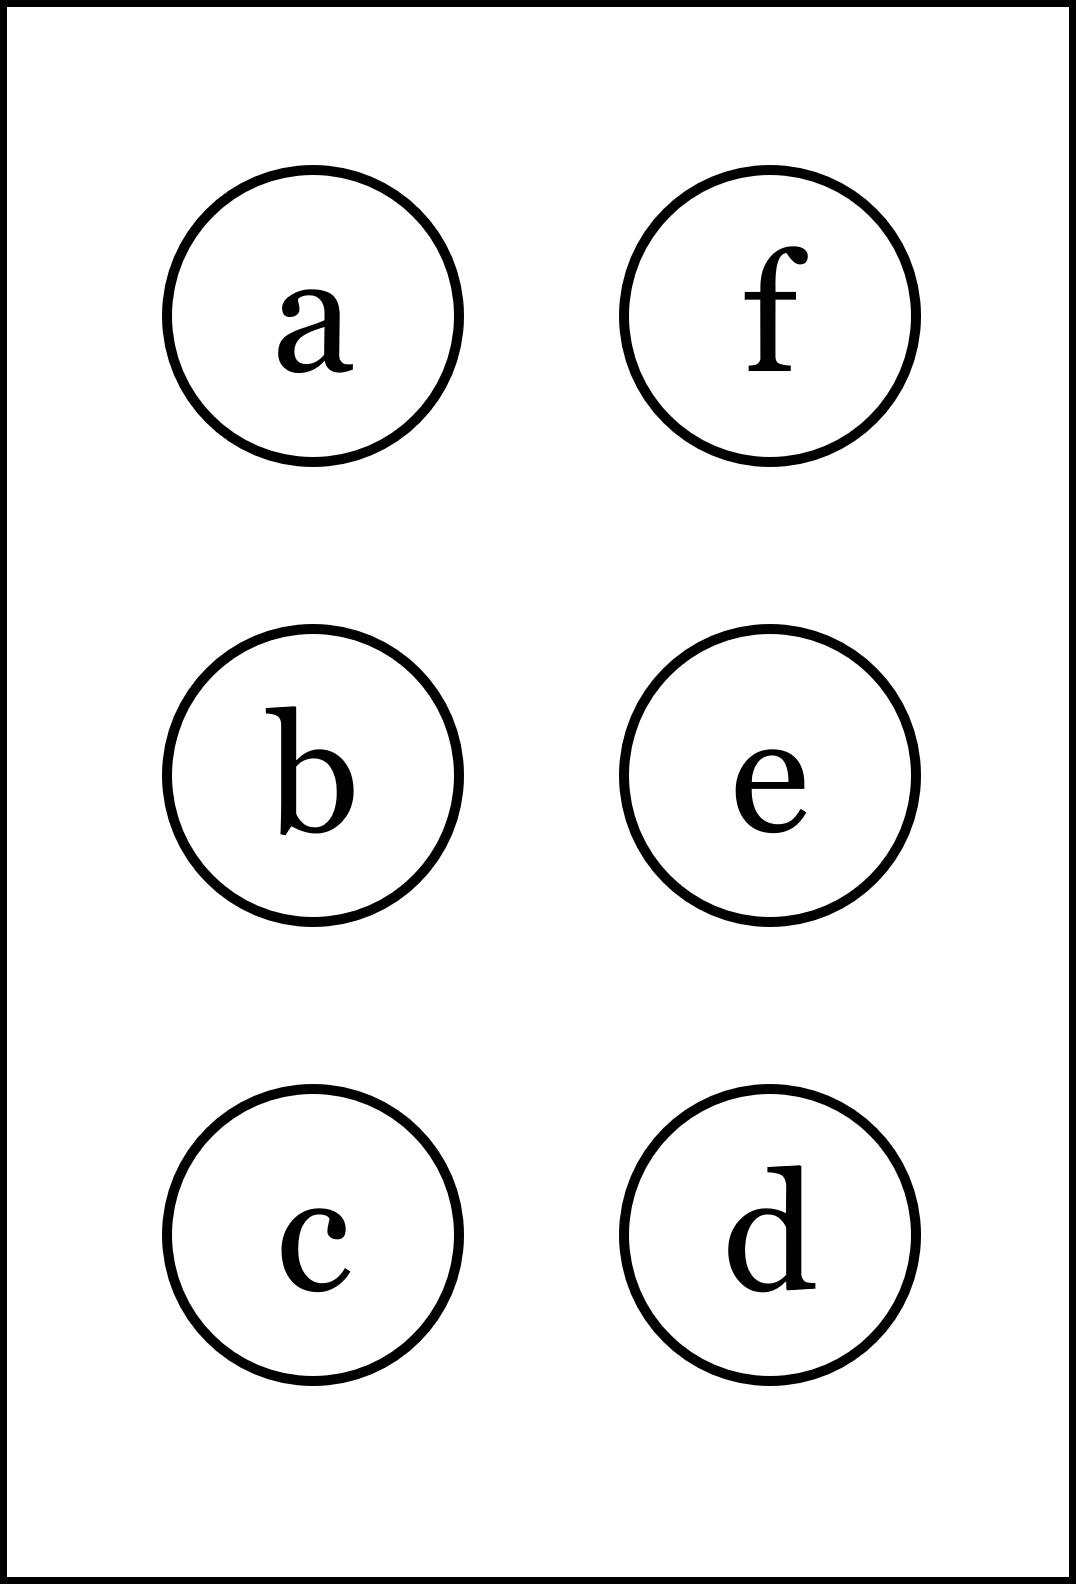
\includegraphics[height=40mm]{../images/braille.png}
{\small Písmeno Braillovej abecedy}
\end{center}
\end{minipage}
\end{center}
\end{minipage}
&
\begin{minipage}[c][104.5mm][t]{0.5\linewidth}
\begin{center}
\vspace{7mm}
{\huge Viazané extrémy, skupina \textit{Alpha $\alpha$} -\romannumeral2}\\[5mm]
\textit{Jméno:}\phantom{xxxxxxxxxxxxxxxxxxxxxxxxxxxxxxxxxxxxxxxxxxxxxxxxxxxxxxxxxxxxxxxxx}\\[5mm]
\begin{minipage}{0.95\linewidth}
\begin{center}
Cílem je najít \textbf{vázané extrémy} funkce $f(x,y)$ zadané v \textbf{(a)} spolu s vazbou (podmínkou). Postupuj podle krokú v \textbf{(b)} až \textbf{(f)}. Pokud se medzivýsledky shodujú s těmi za otazníky,\\tak napravo obarvi příslušející kroužek načerno. \textbf{Spolu odevzdejte výsledné slovo}.
\end{center}
\end{minipage}
\\[1mm]
\begin{minipage}{0.79\linewidth}
\begin{center}
\begin{varwidth}{\linewidth}
\begin{enumerate}
\normalsize
\item $f(x,y)=-5x+12y+3 \enspace , \enspace \mathrm{vazba:} \enspace x^2+y^2=169$\quad \dotfill\; ???\;\dotfill \quad vybarvi
\item Sestav $L(\lambda,x,y)$ a spočti $\pdv{L}{x}=$\quad \dotfill\; ???\;\dotfill \quad $-5+\lambda x$
\item Takisto spočti $\pdv{L}{y}=$\quad \dotfill\; ???\;\dotfill \quad $12+2\lambda y$
\item Z podmínek $\pdv{L}{x}=0 , \pdv{L}{y}=0$ vyjádři $x,y$ v závislosti na $\lambda$.\\ \phantom{xxxxxx}Následne $x,y$ dosaď do vazbové rovnice\\ \phantom{xxxxxx}a vypočti dva výsledky pro $\lambda$.\quad \dotfill\; ???\;\dotfill \quad $\lambda_1+\lambda_2=2$
\item Pomocou $\lambda$ urč dvě dvojice pro $x,y$.\quad \dotfill\; ???\;\dotfill \quad $x_1 x_2 y_1 y_2=3600$
\item Najdi funkční hodnoty pro oba vázané stacionární body\\ \phantom{xxxxxx}a vyber tu najvětší. $f_{\text{max}}(x,y)=$\quad \dotfill\; ???\;\dotfill \quad $171$
\end{enumerate}
\end{varwidth}
\end{center}
\end{minipage}
\begin{minipage}{0.20\linewidth}
\begin{center}
{\Huge\bfseries 2.} \\[2mm]
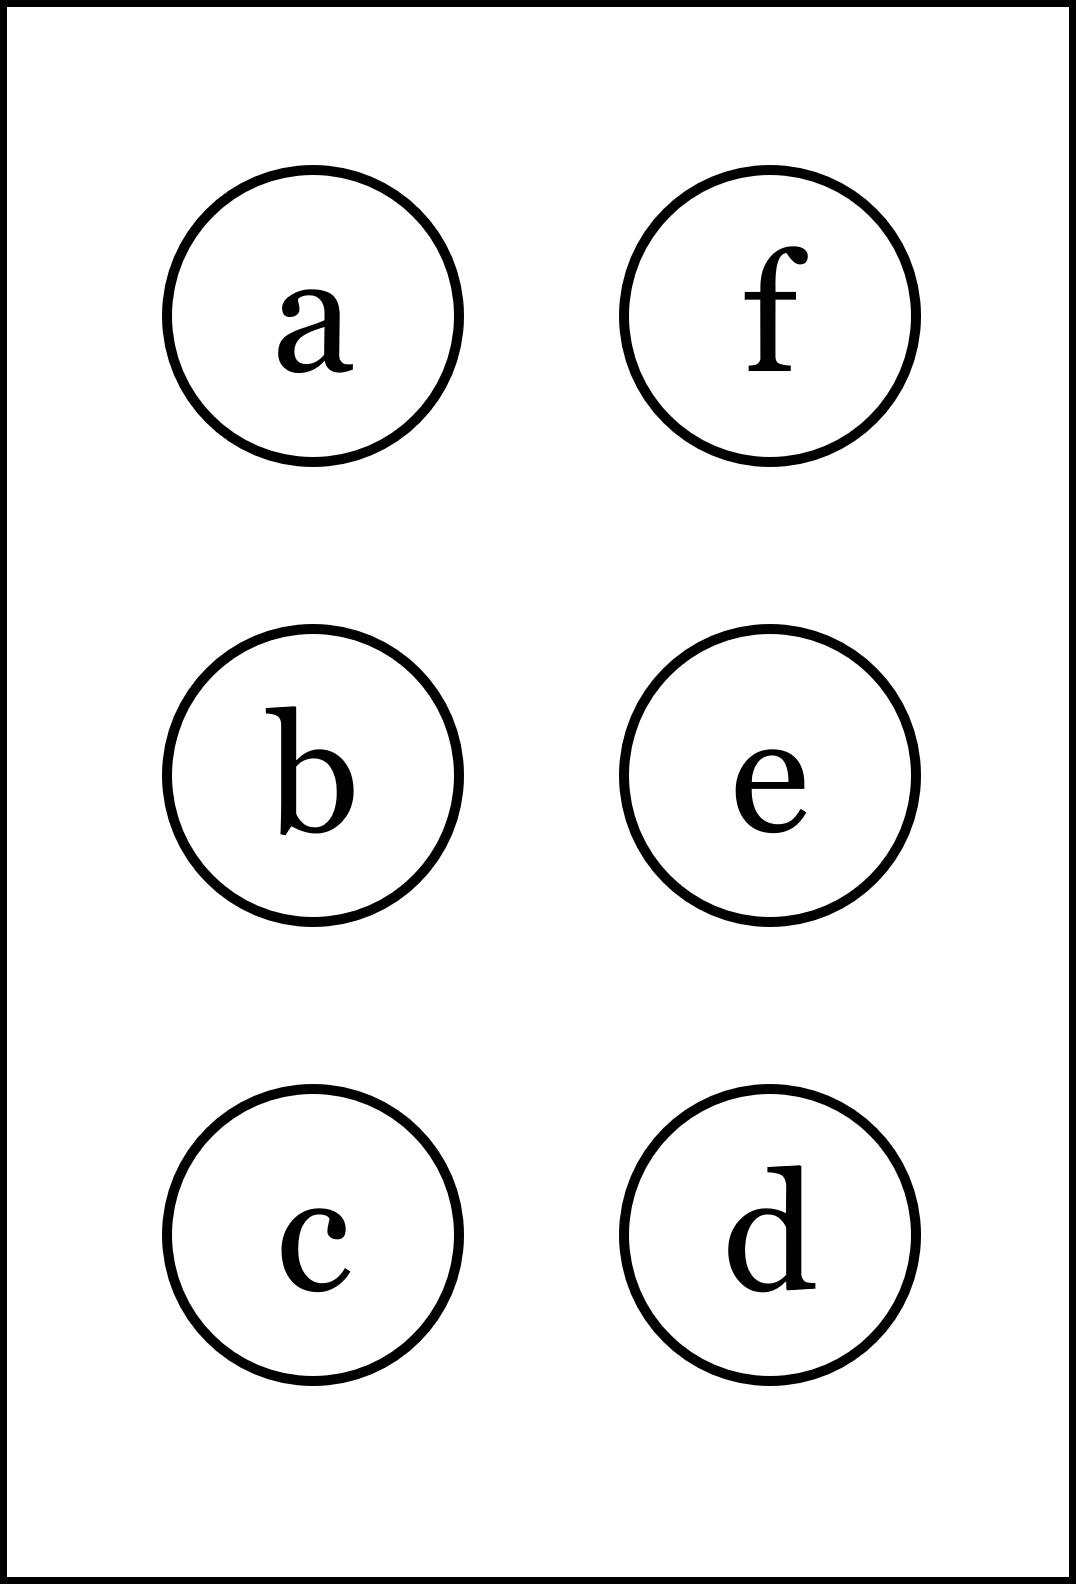
\includegraphics[height=40mm]{../images/braille.png}
{\small Písmeno Braillovej abecedy}
\end{center}
\end{minipage}
\end{center}
\end{minipage}
\\ \hdashline
\begin{minipage}[c][104.5mm][t]{0.5\linewidth}
\begin{center}
\vspace{7mm}
{\huge Viazané extrémy, skupina \textit{Alpha $\alpha$} -\romannumeral3}\\[5mm]
\textit{Jméno:}\phantom{xxxxxxxxxxxxxxxxxxxxxxxxxxxxxxxxxxxxxxxxxxxxxxxxxxxxxxxxxxxxxxxxx}\\[5mm]
\begin{minipage}{0.95\linewidth}
\begin{center}
Cílem je najít \textbf{vázané extrémy} funkce $f(x,y)$ zadané v \textbf{(a)} spolu s vazbou (podmínkou). Postupuj podle krokú v \textbf{(b)} až \textbf{(f)}. Pokud se medzivýsledky shodujú s těmi za otazníky,\\tak napravo obarvi příslušející kroužek načerno. \textbf{Spolu odevzdejte výsledné slovo}.
\end{center}
\end{minipage}
\\[1mm]
\begin{minipage}{0.79\linewidth}
\begin{center}
\begin{varwidth}{\linewidth}
\begin{enumerate}
\normalsize
\item $f(x,y)=6x-8y+3 \enspace , \enspace \mathrm{vazba:} \enspace x^2+y^2=100$\quad \dotfill\; ???\;\dotfill \quad vybarvi
\item Sestav $L(\lambda,x,y)$ a spočti $\pdv{L}{x}=$\quad \dotfill\; ???\;\dotfill \quad $6+2\lambda x$
\item Takisto spočti $\pdv{L}{y}=$\quad \dotfill\; ???\;\dotfill \quad $+8+2\lambda y$
\item Z podmínek $\pdv{L}{x}=0 , \pdv{L}{y}=0$ vyjádři $x,y$ v závislosti na $\lambda$.\\ \phantom{xxxxxx}Následne $x,y$ dosaď do vazbové rovnice\\ \phantom{xxxxxx}a vypočti dva výsledky pro $\lambda$.\quad \dotfill\; ???\;\dotfill \quad $\lambda_1+\lambda_2=-1$
\item Pomocou $\lambda$ urč dvě dvojice pro $x,y$.\quad \dotfill\; ???\;\dotfill \quad $x_1 x_2 y_1 y_2=-288$
\item Najdi funkční hodnoty pro oba vázané stacionární body\\ \phantom{xxxxxx}a vyber tu najvětší. $f_{\text{max}}(x,y)=$\quad \dotfill\; ???\;\dotfill \quad $102$
\end{enumerate}
\end{varwidth}
\end{center}
\end{minipage}
\begin{minipage}{0.20\linewidth}
\begin{center}
{\Huge\bfseries 3.} \\[2mm]
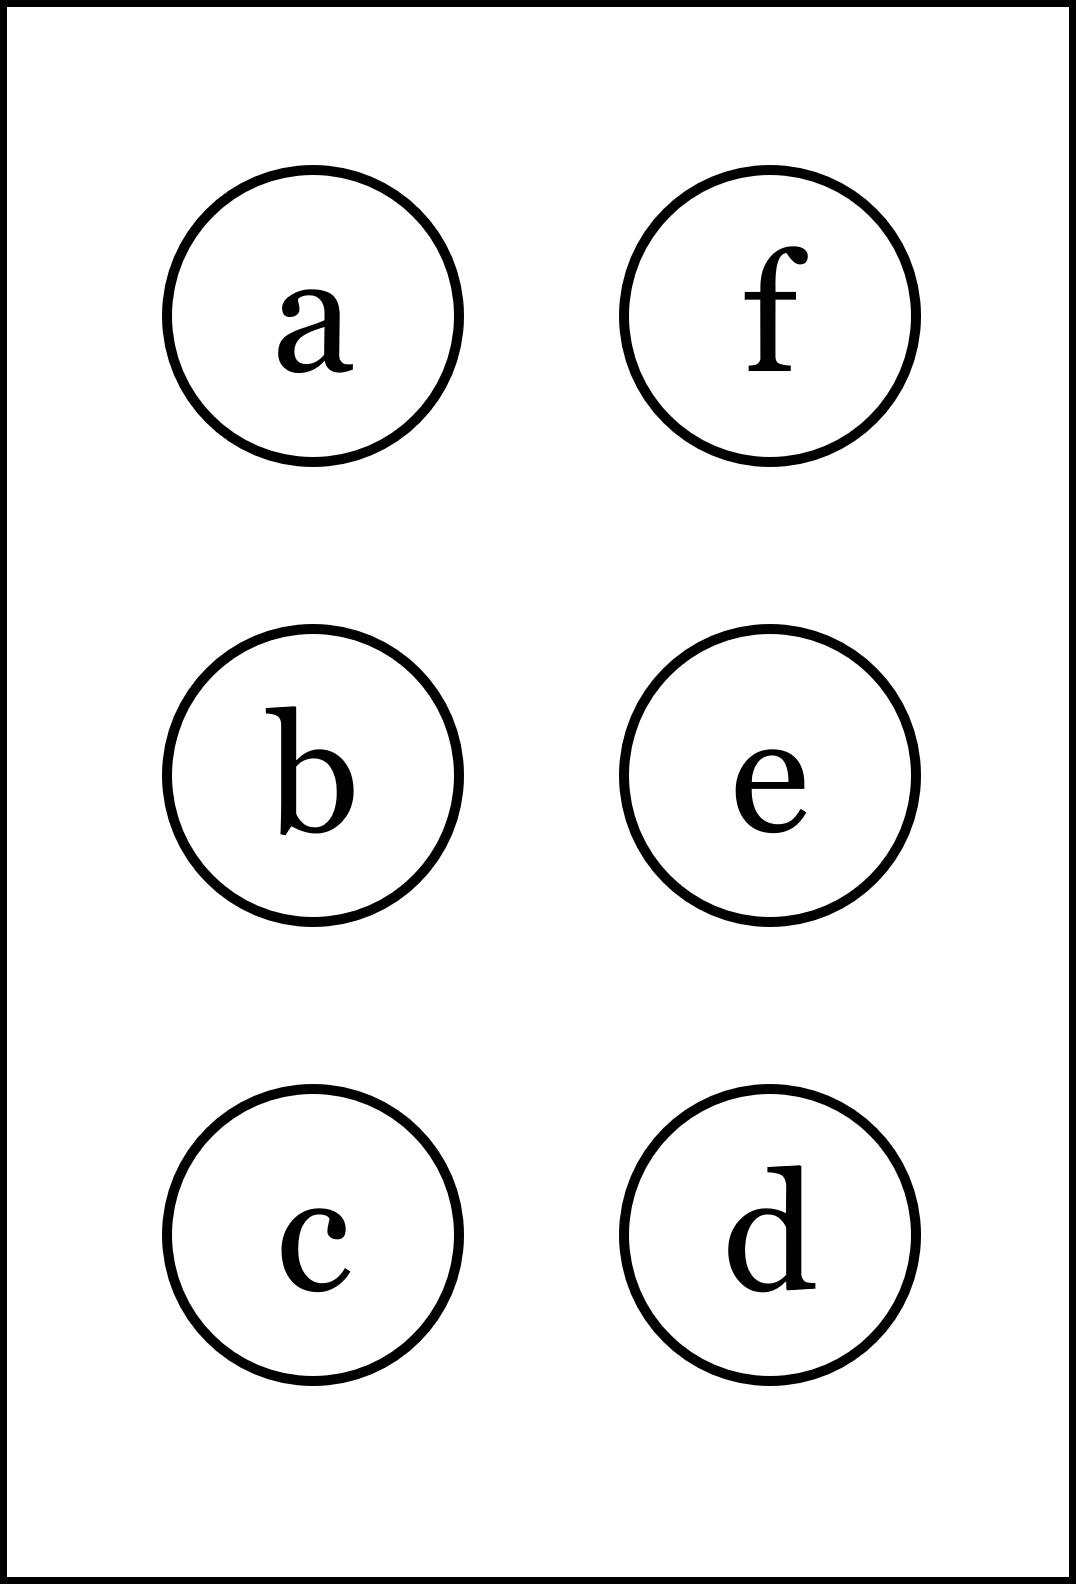
\includegraphics[height=40mm]{../images/braille.png}
{\small Písmeno Braillovej abecedy}
\end{center}
\end{minipage}
\end{center}
\end{minipage}
&
\begin{minipage}[c][104.5mm][t]{0.5\linewidth}
\begin{center}
\vspace{7mm}
{\huge Viazané extrémy, skupina \textit{Alpha $\alpha$} -\romannumeral4}\\[5mm]
\textit{Jméno:}\phantom{xxxxxxxxxxxxxxxxxxxxxxxxxxxxxxxxxxxxxxxxxxxxxxxxxxxxxxxxxxxxxxxxx}\\[5mm]
\begin{minipage}{0.95\linewidth}
\begin{center}
Cílem je najít \textbf{vázané extrémy} funkce $f(x,y)$ zadané v \textbf{(a)} spolu s vazbou (podmínkou). Postupuj podle krokú v \textbf{(b)} až \textbf{(f)}. Pokud se medzivýsledky shodujú s těmi za otazníky,\\tak napravo obarvi příslušející kroužek načerno. \textbf{Spolu odevzdejte výsledné slovo}.
\end{center}
\end{minipage}
\\[1mm]
\begin{minipage}{0.79\linewidth}
\begin{center}
\begin{varwidth}{\linewidth}
\begin{enumerate}
\normalsize
\item $f(x,y)=-10x+24y-3 \enspace , \enspace \mathrm{vazba:} \enspace x^2+y^2=676$\quad \dotfill\; ???\;\dotfill \quad vybarvi
\item Sestav $L(\lambda,x,y)$ a spočti $\pdv{L}{x}=$\quad \dotfill\; ???\;\dotfill \quad $-10+2\lambda x$
\item Takisto spočti $\pdv{L}{y}=$\quad \dotfill\; ???\;\dotfill \quad $24+2\lambda y$
\item Z podmínek $\pdv{L}{x}=0 , \pdv{L}{y}=0$ vyjádři $x,y$ v závislosti na $\lambda$.\\ \phantom{xxxxxx}Následne $x,y$ dosaď do vazbové rovnice\\ \phantom{xxxxxx}a vypočti dva výsledky pro $\lambda$.\quad \dotfill\; ???\;\dotfill \quad $\lambda_1+\lambda_2=2$
\item Pomocou $\lambda$ urč dvě dvojice pro $x,y$.\quad \dotfill\; ???\;\dotfill \quad $x_1 x_2 y_1 y_2=57600$
\item Najdi funkční hodnoty pro oba vázané stacionární body\\ \phantom{xxxxxx}a vyber tu najvětší. $f_{\text{max}}(x,y)=$\quad \dotfill\; ???\;\dotfill \quad $672$
\end{enumerate}
\end{varwidth}
\end{center}
\end{minipage}
\begin{minipage}{0.20\linewidth}
\begin{center}
{\Huge\bfseries 4.} \\[2mm]
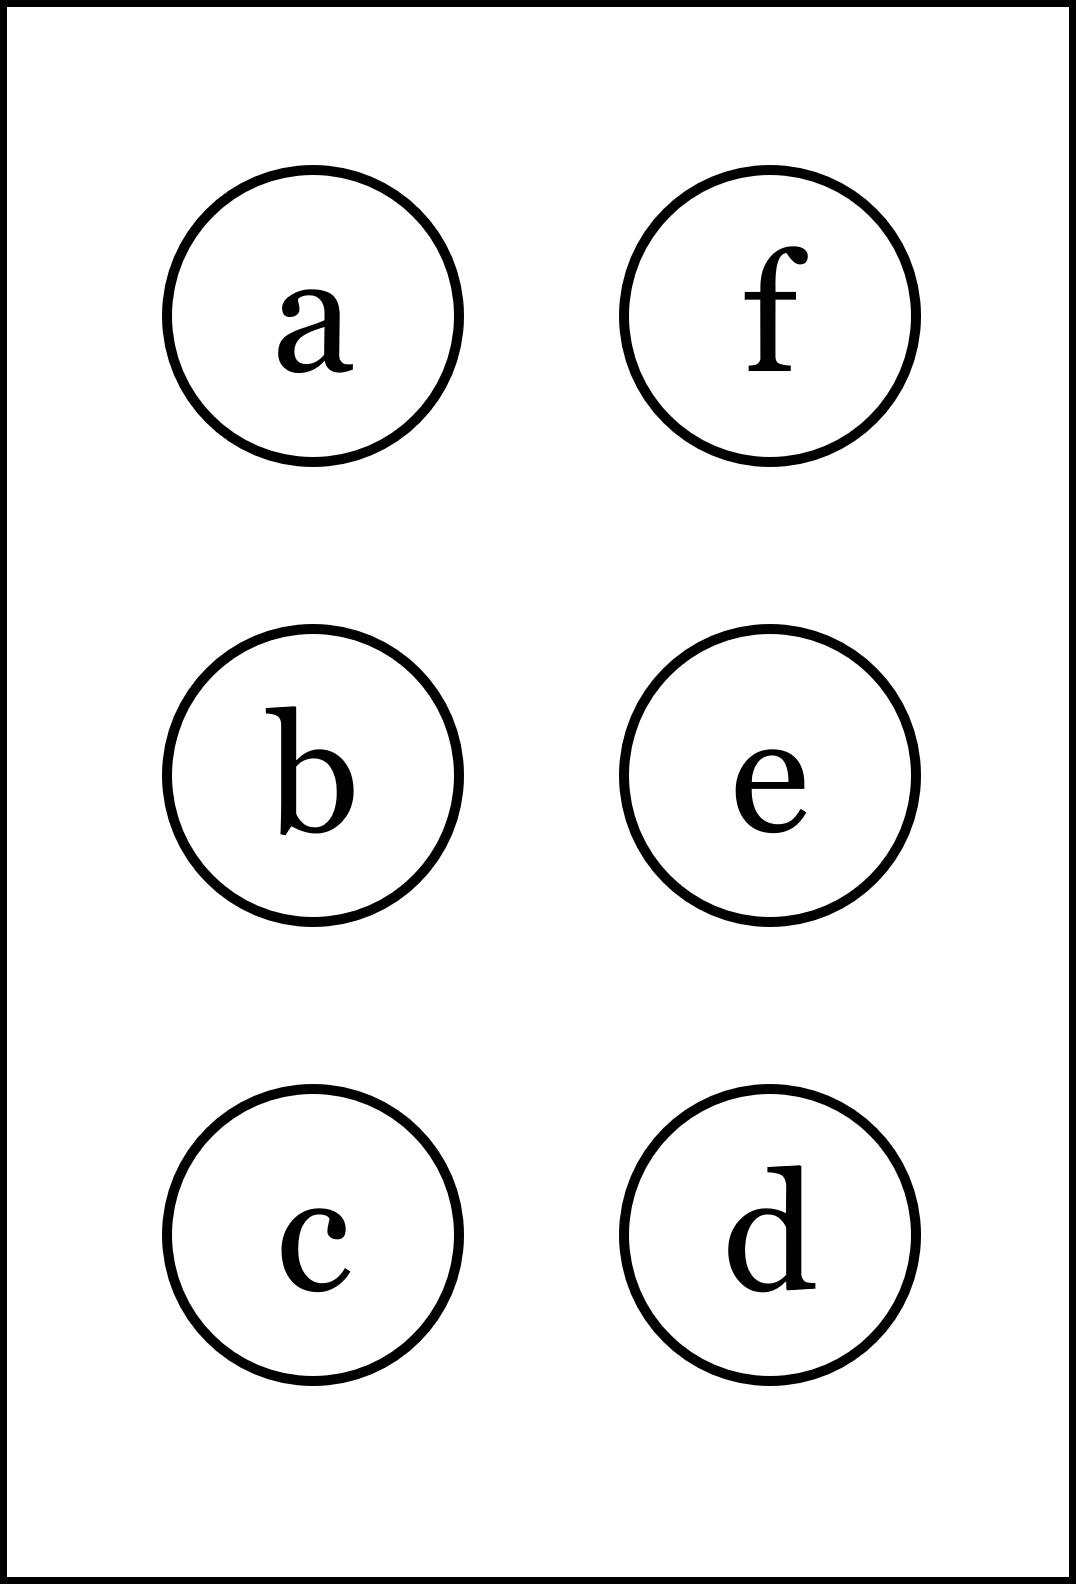
\includegraphics[height=40mm]{../images/braille.png}
{\small Písmeno Braillovej abecedy}
\end{center}
\end{minipage}
\end{center}
\end{minipage}
%
\end{tabular}
\newpage
\thispagestyle{empty}
\begin{tabular}{c:c}
\begin{minipage}[c][104.5mm][t]{0.5\linewidth}
\begin{center}
\vspace{7mm}
{\huge Viazané extrémy, skupina \textit{Beta $\beta$} -\romannumeral1}\\[5mm]
\textit{Jméno:}\phantom{xxxxxxxxxxxxxxxxxxxxxxxxxxxxxxxxxxxxxxxxxxxxxxxxxxxxxxxxxxxxxxxxx}\\[5mm]
\begin{minipage}{0.95\linewidth}
\begin{center}
Cílem je najít \textbf{vázané extrémy} funkce $f(x,y)$ zadané v \textbf{(a)} spolu s vazbou (podmínkou). Postupuj podle krokú v \textbf{(b)} až \textbf{(f)}. Pokud se medzivýsledky shodujú s těmi za otazníky,\\tak napravo obarvi příslušející kroužek načerno. \textbf{Spolu odevzdejte výsledné slovo}.
\end{center}
\end{minipage}
\\[1mm]
\begin{minipage}{0.79\linewidth}
\begin{center}
\begin{varwidth}{\linewidth}
\begin{enumerate}
\normalsize
\item $f(x,y)=-3x-4y-5 \enspace , \enspace \mathrm{vazba:} \enspace x^2+y^2=25$\quad \dotfill\; ???\;\dotfill \quad nebarvi
\item Sestav $L(\lambda,x,y)$ a spočti $\pdv{L}{x}=$\quad \dotfill\; ???\;\dotfill \quad $-3+\lambda x$
\item Takisto spočti $\pdv{L}{y}=$\quad \dotfill\; ???\;\dotfill \quad $-4+2\lambda y$
\item Z podmínek $\pdv{L}{x}=0 , \pdv{L}{y}=0$ vyjádři $x,y$ v závislosti na $\lambda$.\\ \phantom{xxxxxx}Následne $x,y$ dosaď do vazbové rovnice\\ \phantom{xxxxxx}a vypočti dva výsledky pro $\lambda$.\quad \dotfill\; ???\;\dotfill \quad $\lambda_1+\lambda_2=0$
\item Pomocou $\lambda$ urč dvě dvojice pro $x,y$.\quad \dotfill\; ???\;\dotfill \quad $x_1 x_2 y_1 y_2=-36$
\item Najdi funkční hodnoty pro oba vázané stacionární body\\ \phantom{xxxxxx}a vyber tu najvětší. $f_{\text{max}}(x,y)=$\quad \dotfill\; ???\;\dotfill \quad $20$
\end{enumerate}
\end{varwidth}
\end{center}
\end{minipage}
\begin{minipage}{0.20\linewidth}
\begin{center}
{\Huge\bfseries 1.} \\[2mm]
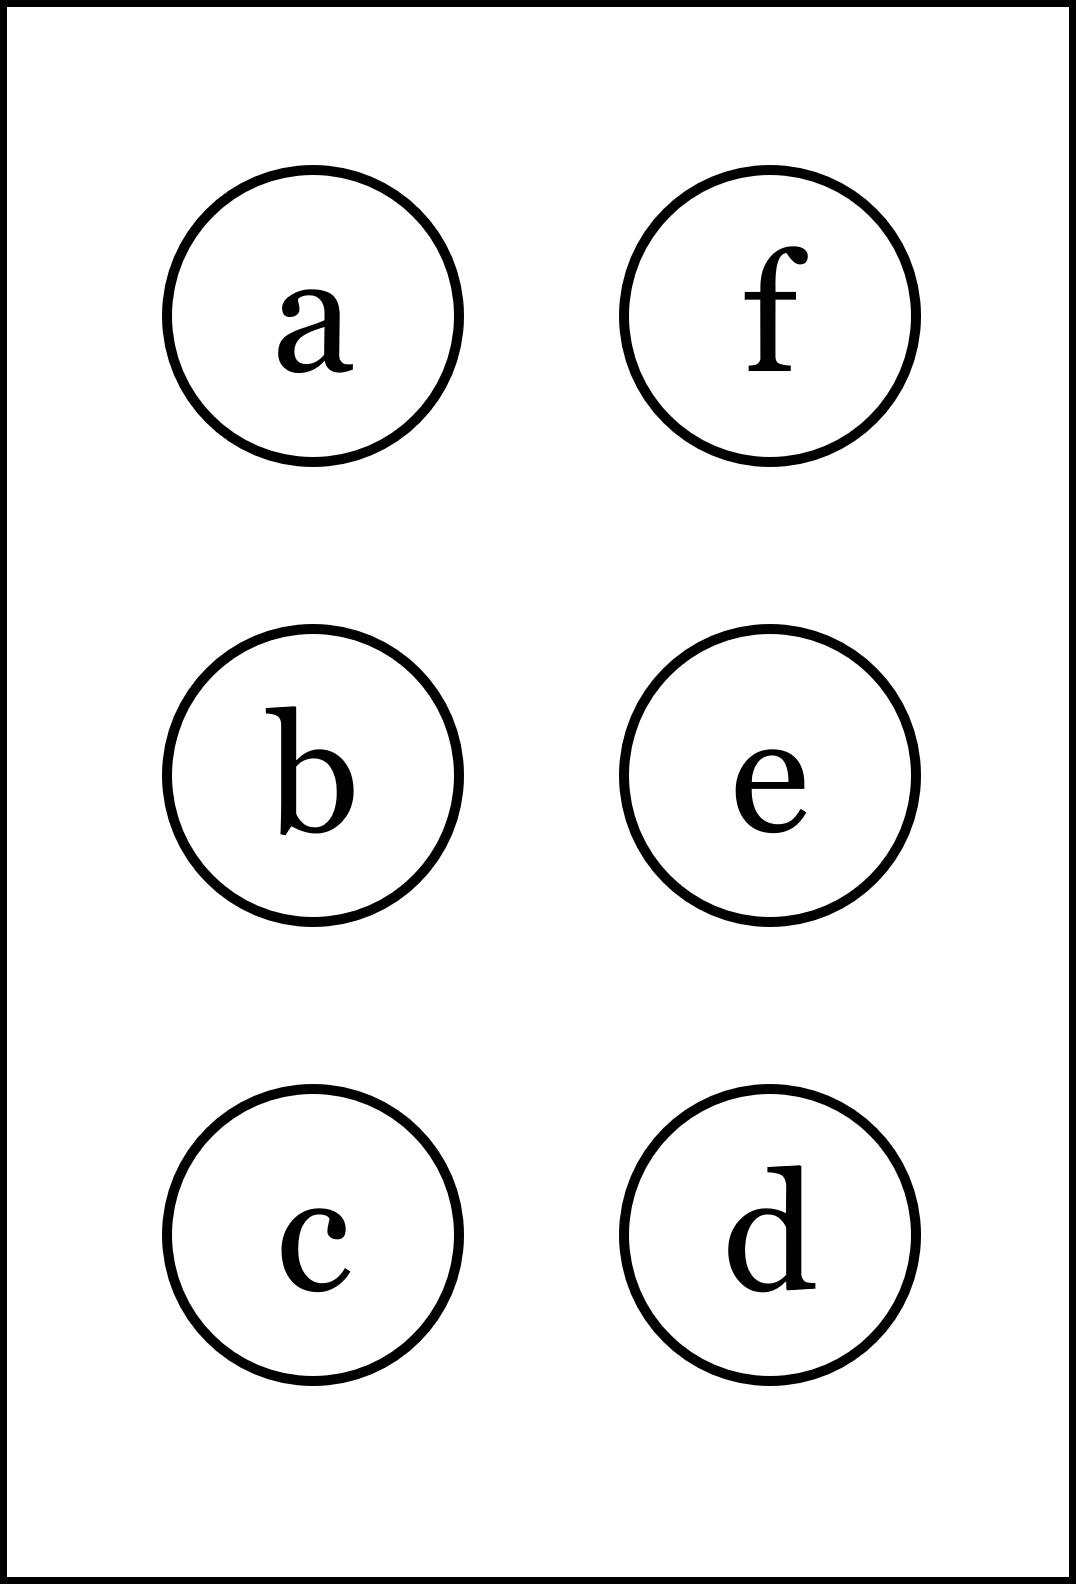
\includegraphics[height=40mm]{../images/braille.png}
{\small Písmeno Braillovej abecedy}
\end{center}
\end{minipage}
\end{center}
\end{minipage}
&
\begin{minipage}[c][104.5mm][t]{0.5\linewidth}
\begin{center}
\vspace{7mm}
{\huge Viazané extrémy, skupina \textit{Beta $\beta$} -\romannumeral2}\\[5mm]
\textit{Jméno:}\phantom{xxxxxxxxxxxxxxxxxxxxxxxxxxxxxxxxxxxxxxxxxxxxxxxxxxxxxxxxxxxxxxxxx}\\[5mm]
\begin{minipage}{0.95\linewidth}
\begin{center}
Cílem je najít \textbf{vázané extrémy} funkce $f(x,y)$ zadané v \textbf{(a)} spolu s vazbou (podmínkou). Postupuj podle krokú v \textbf{(b)} až \textbf{(f)}. Pokud se medzivýsledky shodujú s těmi za otazníky,\\tak napravo obarvi příslušející kroužek načerno. \textbf{Spolu odevzdejte výsledné slovo}.
\end{center}
\end{minipage}
\\[1mm]
\begin{minipage}{0.79\linewidth}
\begin{center}
\begin{varwidth}{\linewidth}
\begin{enumerate}
\normalsize
\item $f(x,y)=-5x+12y+4 \enspace , \enspace \mathrm{vazba:} \enspace x^2+y^2=169$\quad \dotfill\; ???\;\dotfill \quad nebarvi
\item Sestav $L(\lambda,x,y)$ a spočti $\pdv{L}{x}=$\quad \dotfill\; ???\;\dotfill \quad $-5+2\lambda x$
\item Takisto spočti $\pdv{L}{y}=$\quad \dotfill\; ???\;\dotfill \quad $12+2\lambda y$
\item Z podmínek $\pdv{L}{x}=0 , \pdv{L}{y}=0$ vyjádři $x,y$ v závislosti na $\lambda$.\\ \phantom{xxxxxx}Následne $x,y$ dosaď do vazbové rovnice\\ \phantom{xxxxxx}a vypočti dva výsledky pro $\lambda$.\quad \dotfill\; ???\;\dotfill \quad $\lambda_1+\lambda_2=-1$
\item Pomocou $\lambda$ urč dvě dvojice pro $x,y$.\quad \dotfill\; ???\;\dotfill \quad $x_1 x_2 y_1 y_2=300$
\item Najdi funkční hodnoty pro oba vázané stacionární body\\ \phantom{xxxxxx}a vyber tu najvětší. $f_{\text{max}}(x,y)=$\quad \dotfill\; ???\;\dotfill \quad $173$
\end{enumerate}
\end{varwidth}
\end{center}
\end{minipage}
\begin{minipage}{0.20\linewidth}
\begin{center}
{\Huge\bfseries 2.} \\[2mm]
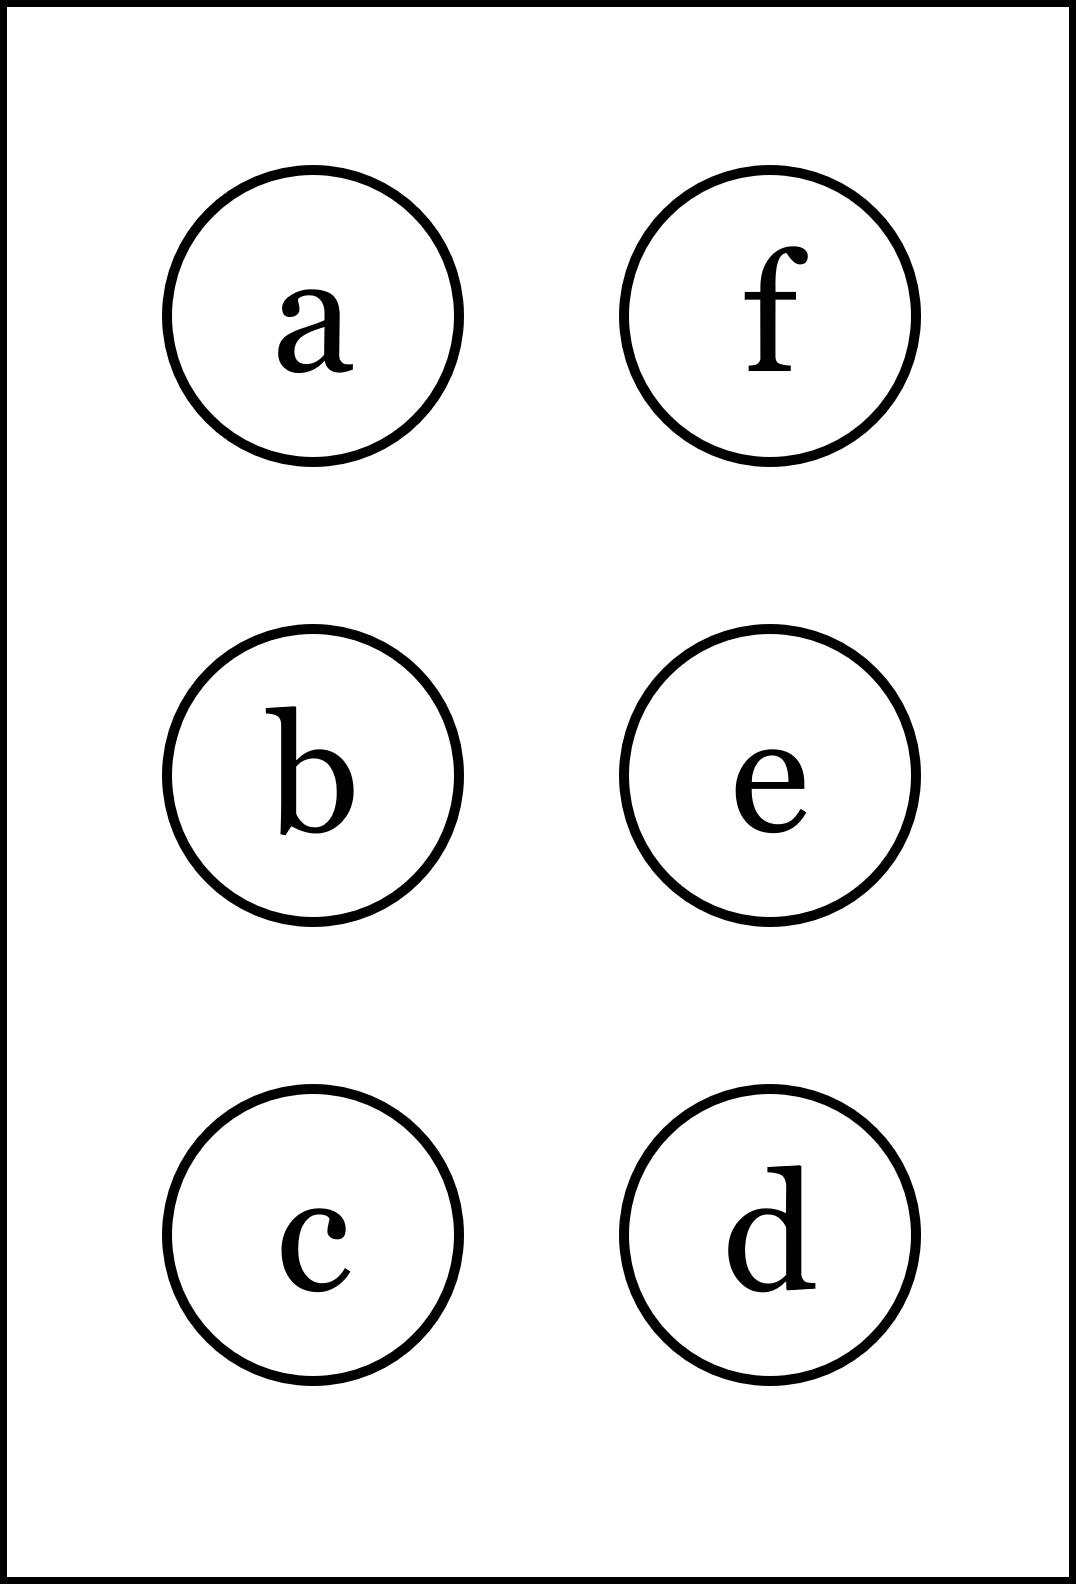
\includegraphics[height=40mm]{../images/braille.png}
{\small Písmeno Braillovej abecedy}
\end{center}
\end{minipage}
\end{center}
\end{minipage}
\\ \hdashline
\begin{minipage}[c][104.5mm][t]{0.5\linewidth}
\begin{center}
\vspace{7mm}
{\huge Viazané extrémy, skupina \textit{Beta $\beta$} -\romannumeral3}\\[5mm]
\textit{Jméno:}\phantom{xxxxxxxxxxxxxxxxxxxxxxxxxxxxxxxxxxxxxxxxxxxxxxxxxxxxxxxxxxxxxxxxx}\\[5mm]
\begin{minipage}{0.95\linewidth}
\begin{center}
Cílem je najít \textbf{vázané extrémy} funkce $f(x,y)$ zadané v \textbf{(a)} spolu s vazbou (podmínkou). Postupuj podle krokú v \textbf{(b)} až \textbf{(f)}. Pokud se medzivýsledky shodujú s těmi za otazníky,\\tak napravo obarvi příslušející kroužek načerno. \textbf{Spolu odevzdejte výsledné slovo}.
\end{center}
\end{minipage}
\\[1mm]
\begin{minipage}{0.79\linewidth}
\begin{center}
\begin{varwidth}{\linewidth}
\begin{enumerate}
\normalsize
\item $f(x,y)=6x+8y+1 \enspace , \enspace \mathrm{vazba:} \enspace x^2+y^2=100$\quad \dotfill\; ???\;\dotfill \quad nebarvi
\item Sestav $L(\lambda,x,y)$ a spočti $\pdv{L}{x}=$\quad \dotfill\; ???\;\dotfill \quad $6+2\lambda x$
\item Takisto spočti $\pdv{L}{y}=$\quad \dotfill\; ???\;\dotfill \quad $8+2\lambda y$
\item Z podmínek $\pdv{L}{x}=0 , \pdv{L}{y}=0$ vyjádři $x,y$ v závislosti na $\lambda$.\\ \phantom{xxxxxx}Následne $x,y$ dosaď do vazbové rovnice\\ \phantom{xxxxxx}a vypočti dva výsledky pro $\lambda$.\quad \dotfill\; ???\;\dotfill \quad $\lambda_1+\lambda_2=1$
\item Pomocou $\lambda$ urč dvě dvojice pro $x,y$.\quad \dotfill\; ???\;\dotfill \quad $x_1 x_2 y_1 y_2=2304$
\item Najdi funkční hodnoty pro oba vázané stacionární body\\ \phantom{xxxxxx}a vyber tu najvětší. $f_{\text{max}}(x,y)=$\quad \dotfill\; ???\;\dotfill \quad $101$
\end{enumerate}
\end{varwidth}
\end{center}
\end{minipage}
\begin{minipage}{0.20\linewidth}
\begin{center}
{\Huge\bfseries 3.} \\[2mm]
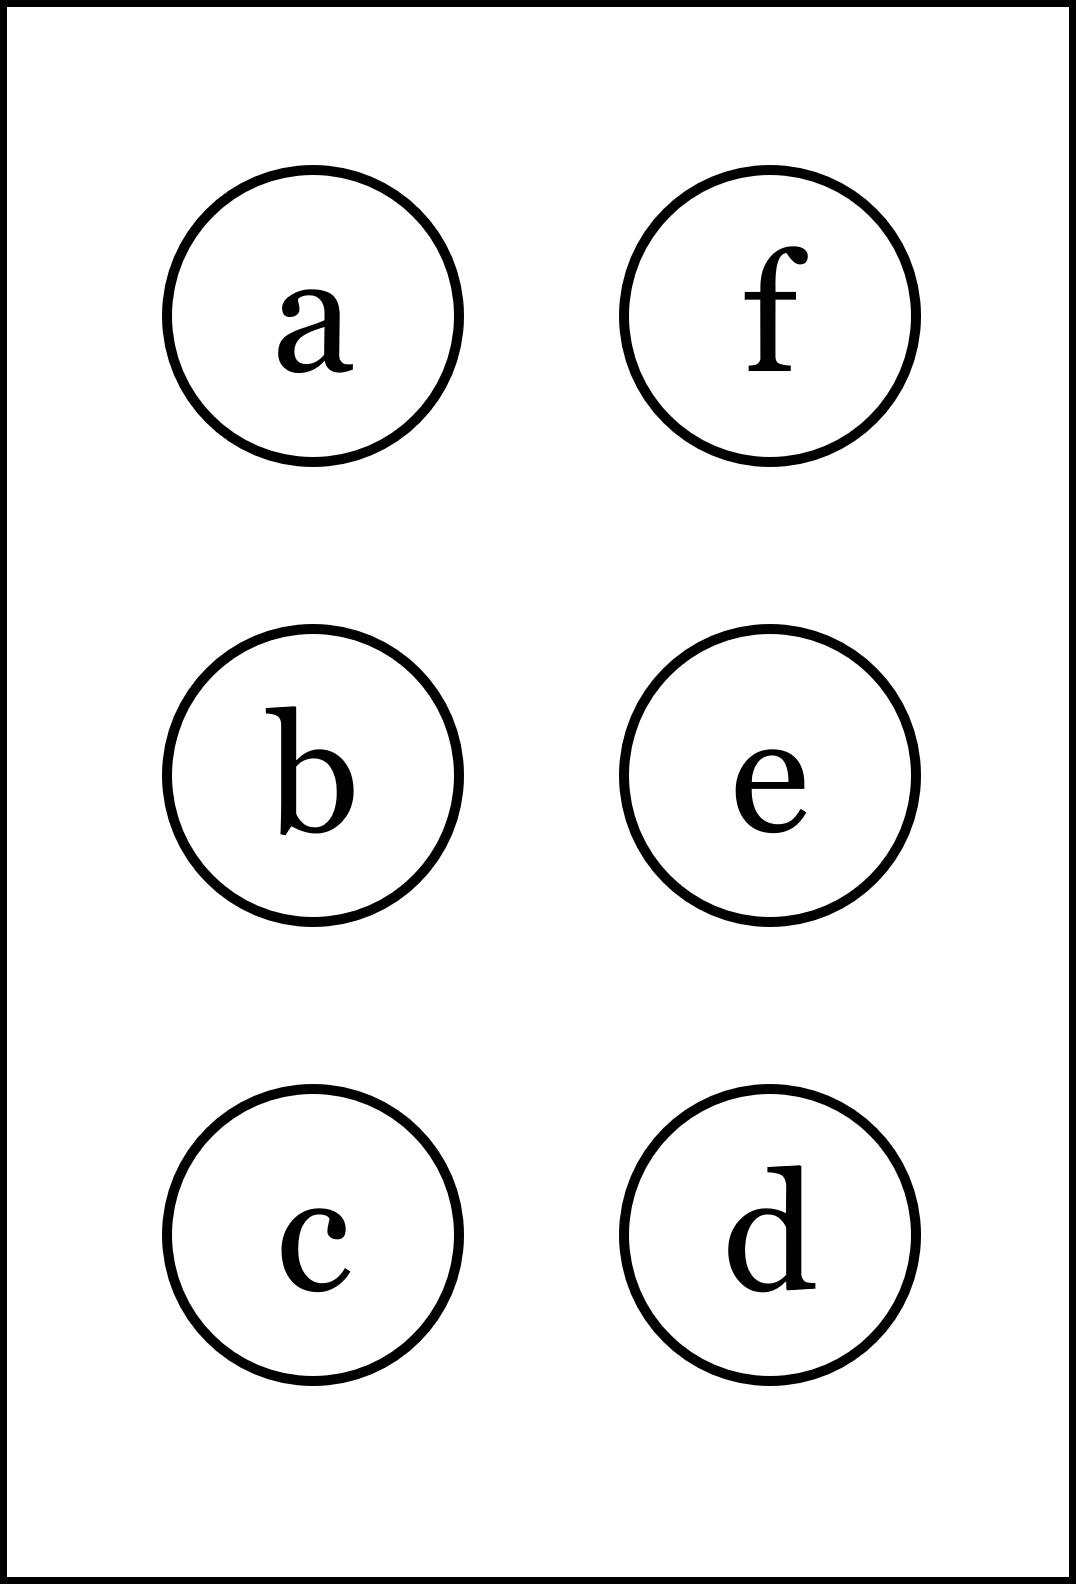
\includegraphics[height=40mm]{../images/braille.png}
{\small Písmeno Braillovej abecedy}
\end{center}
\end{minipage}
\end{center}
\end{minipage}
&
\begin{minipage}[c][104.5mm][t]{0.5\linewidth}
\begin{center}
\vspace{7mm}
{\huge Viazané extrémy, skupina \textit{Beta $\beta$} -\romannumeral4}\\[5mm]
\textit{Jméno:}\phantom{xxxxxxxxxxxxxxxxxxxxxxxxxxxxxxxxxxxxxxxxxxxxxxxxxxxxxxxxxxxxxxxxx}\\[5mm]
\begin{minipage}{0.95\linewidth}
\begin{center}
Cílem je najít \textbf{vázané extrémy} funkce $f(x,y)$ zadané v \textbf{(a)} spolu s vazbou (podmínkou). Postupuj podle krokú v \textbf{(b)} až \textbf{(f)}. Pokud se medzivýsledky shodujú s těmi za otazníky,\\tak napravo obarvi příslušející kroužek načerno. \textbf{Spolu odevzdejte výsledné slovo}.
\end{center}
\end{minipage}
\\[1mm]
\begin{minipage}{0.79\linewidth}
\begin{center}
\begin{varwidth}{\linewidth}
\begin{enumerate}
\normalsize
\item $f(x,y)=10x+24y+5 \enspace , \enspace \mathrm{vazba:} \enspace x^2+y^2=676$\quad \dotfill\; ???\;\dotfill \quad nebarvi
\item Sestav $L(\lambda,x,y)$ a spočti $\pdv{L}{x}=$\quad \dotfill\; ???\;\dotfill \quad $10+\lambda x$
\item Takisto spočti $\pdv{L}{y}=$\quad \dotfill\; ???\;\dotfill \quad $24+2\lambda y$
\item Z podmínek $\pdv{L}{x}=0 , \pdv{L}{y}=0$ vyjádři $x,y$ v závislosti na $\lambda$.\\ \phantom{xxxxxx}Následne $x,y$ dosaď do vazbové rovnice\\ \phantom{xxxxxx}a vypočti dva výsledky pro $\lambda$.\quad \dotfill\; ???\;\dotfill \quad $\lambda_1+\lambda_2=1$
\item Pomocou $\lambda$ urč dvě dvojice pro $x,y$.\quad \dotfill\; ???\;\dotfill \quad $x_1 x_2 y_1 y_2=2400$
\item Najdi funkční hodnoty pro oba vázané stacionární body\\ \phantom{xxxxxx}a vyber tu najvětší. $f_{\text{max}}(x,y)=$\quad \dotfill\; ???\;\dotfill \quad $681$
\end{enumerate}
\end{varwidth}
\end{center}
\end{minipage}
\begin{minipage}{0.20\linewidth}
\begin{center}
{\Huge\bfseries 4.} \\[2mm]
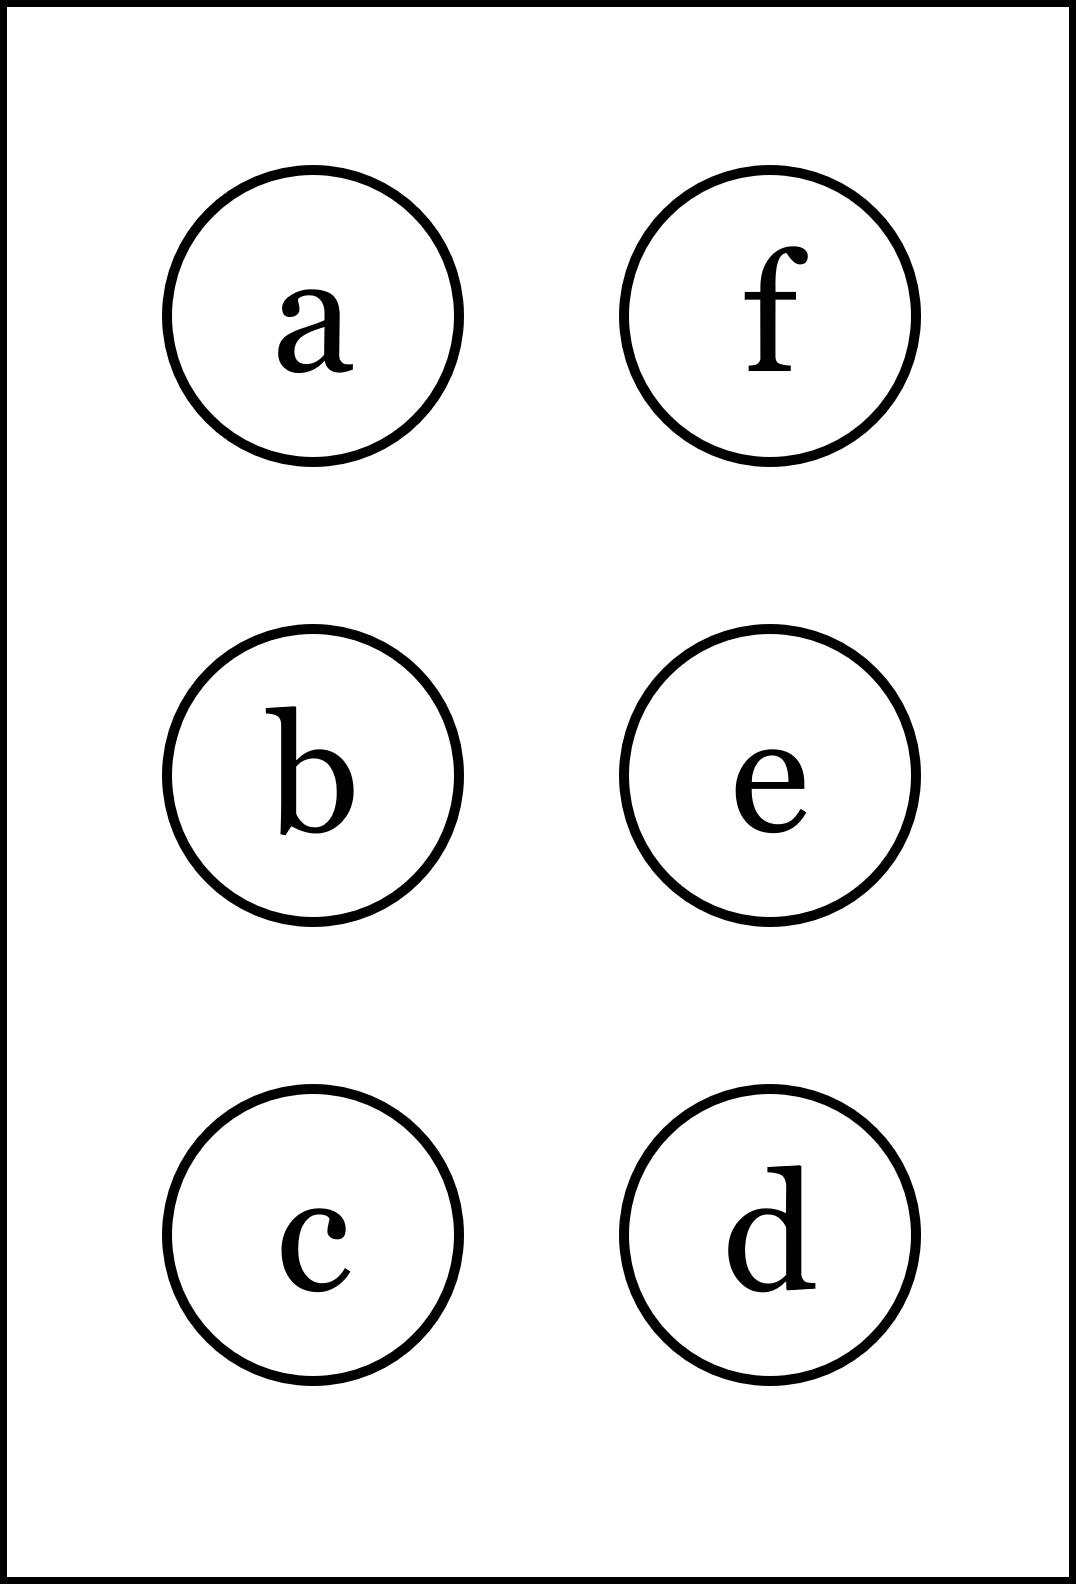
\includegraphics[height=40mm]{../images/braille.png}
{\small Písmeno Braillovej abecedy}
\end{center}
\end{minipage}
\end{center}
\end{minipage}
%
\end{tabular}
\newpage
\thispagestyle{empty}
\begin{tabular}{c:c}
\begin{minipage}[c][104.5mm][t]{0.5\linewidth}
\begin{center}
\vspace{7mm}
{\huge Viazané extrémy, skupina \textit{Gamma $\gamma$} -\romannumeral1}\\[5mm]
\textit{Jméno:}\phantom{xxxxxxxxxxxxxxxxxxxxxxxxxxxxxxxxxxxxxxxxxxxxxxxxxxxxxxxxxxxxxxxxx}\\[5mm]
\begin{minipage}{0.95\linewidth}
\begin{center}
Cílem je najít \textbf{vázané extrémy} funkce $f(x,y)$ zadané v \textbf{(a)} spolu s vazbou (podmínkou). Postupuj podle krokú v \textbf{(b)} až \textbf{(f)}. Pokud se medzivýsledky shodujú s těmi za otazníky,\\tak napravo obarvi příslušející kroužek načerno. \textbf{Spolu odevzdejte výsledné slovo}.
\end{center}
\end{minipage}
\\[1mm]
\begin{minipage}{0.79\linewidth}
\begin{center}
\begin{varwidth}{\linewidth}
\begin{enumerate}
\normalsize
\item $f(x,y)=3x+4y+2 \enspace , \enspace \mathrm{vazba:} \enspace x^2+y^2=25$\quad \dotfill\; ???\;\dotfill \quad vybarvi
\item Sestav $L(\lambda,x,y)$ a spočti $\pdv{L}{x}=$\quad \dotfill\; ???\;\dotfill \quad $3+\lambda x$
\item Takisto spočti $\pdv{L}{y}=$\quad \dotfill\; ???\;\dotfill \quad $-4+2\lambda y$
\item Z podmínek $\pdv{L}{x}=0 , \pdv{L}{y}=0$ vyjádři $x,y$ v závislosti na $\lambda$.\\ \phantom{xxxxxx}Následne $x,y$ dosaď do vazbové rovnice\\ \phantom{xxxxxx}a vypočti dva výsledky pro $\lambda$.\quad \dotfill\; ???\;\dotfill \quad $\lambda_1+\lambda_2=0$
\item Pomocou $\lambda$ urč dvě dvojice pro $x,y$.\quad \dotfill\; ???\;\dotfill \quad $x_1 x_2 y_1 y_2=144$
\item Najdi funkční hodnoty pro oba vázané stacionární body\\ \phantom{xxxxxx}a vyber tu najvětší. $f_{\text{max}}(x,y)=$\quad \dotfill\; ???\;\dotfill \quad $26$
\end{enumerate}
\end{varwidth}
\end{center}
\end{minipage}
\begin{minipage}{0.20\linewidth}
\begin{center}
{\Huge\bfseries 1.} \\[2mm]
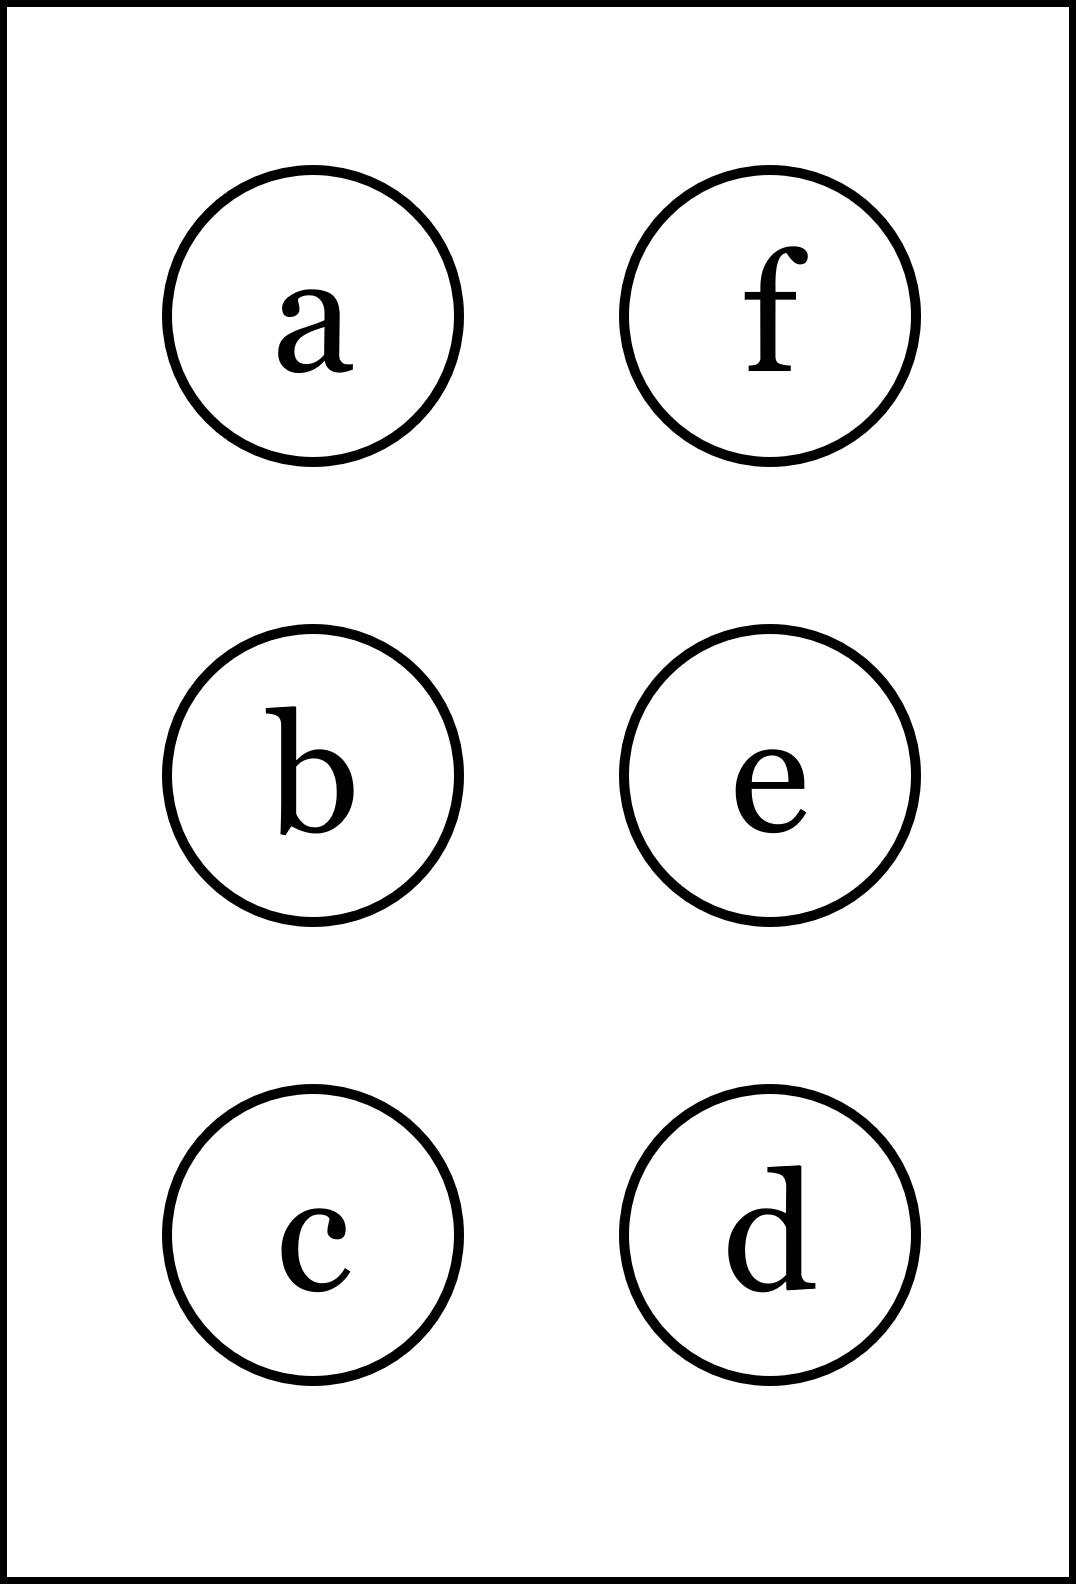
\includegraphics[height=40mm]{../images/braille.png}
{\small Písmeno Braillovej abecedy}
\end{center}
\end{minipage}
\end{center}
\end{minipage}
&
\begin{minipage}[c][104.5mm][t]{0.5\linewidth}
\begin{center}
\vspace{7mm}
{\huge Viazané extrémy, skupina \textit{Gamma $\gamma$} -\romannumeral2}\\[5mm]
\textit{Jméno:}\phantom{xxxxxxxxxxxxxxxxxxxxxxxxxxxxxxxxxxxxxxxxxxxxxxxxxxxxxxxxxxxxxxxxx}\\[5mm]
\begin{minipage}{0.95\linewidth}
\begin{center}
Cílem je najít \textbf{vázané extrémy} funkce $f(x,y)$ zadané v \textbf{(a)} spolu s vazbou (podmínkou). Postupuj podle krokú v \textbf{(b)} až \textbf{(f)}. Pokud se medzivýsledky shodujú s těmi za otazníky,\\tak napravo obarvi příslušející kroužek načerno. \textbf{Spolu odevzdejte výsledné slovo}.
\end{center}
\end{minipage}
\\[1mm]
\begin{minipage}{0.79\linewidth}
\begin{center}
\begin{varwidth}{\linewidth}
\begin{enumerate}
\normalsize
\item $f(x,y)=5x-12y+1 \enspace , \enspace \mathrm{vazba:} \enspace x^2+y^2=169$\quad \dotfill\; ???\;\dotfill \quad vybarvi
\item Sestav $L(\lambda,x,y)$ a spočti $\pdv{L}{x}=$\quad \dotfill\; ???\;\dotfill \quad $5+\lambda x$
\item Takisto spočti $\pdv{L}{y}=$\quad \dotfill\; ???\;\dotfill \quad $-12+2\lambda y$
\item Z podmínek $\pdv{L}{x}=0 , \pdv{L}{y}=0$ vyjádři $x,y$ v závislosti na $\lambda$.\\ \phantom{xxxxxx}Následne $x,y$ dosaď do vazbové rovnice\\ \phantom{xxxxxx}a vypočti dva výsledky pro $\lambda$.\quad \dotfill\; ???\;\dotfill \quad $\lambda_1+\lambda_2=1$
\item Pomocou $\lambda$ urč dvě dvojice pro $x,y$.\quad \dotfill\; ???\;\dotfill \quad $x_1 x_2 y_1 y_2=3600$
\item Najdi funkční hodnoty pro oba vázané stacionární body\\ \phantom{xxxxxx}a vyber tu najvětší. $f_{\text{max}}(x,y)=$\quad \dotfill\; ???\;\dotfill \quad $170$
\end{enumerate}
\end{varwidth}
\end{center}
\end{minipage}
\begin{minipage}{0.20\linewidth}
\begin{center}
{\Huge\bfseries 2.} \\[2mm]
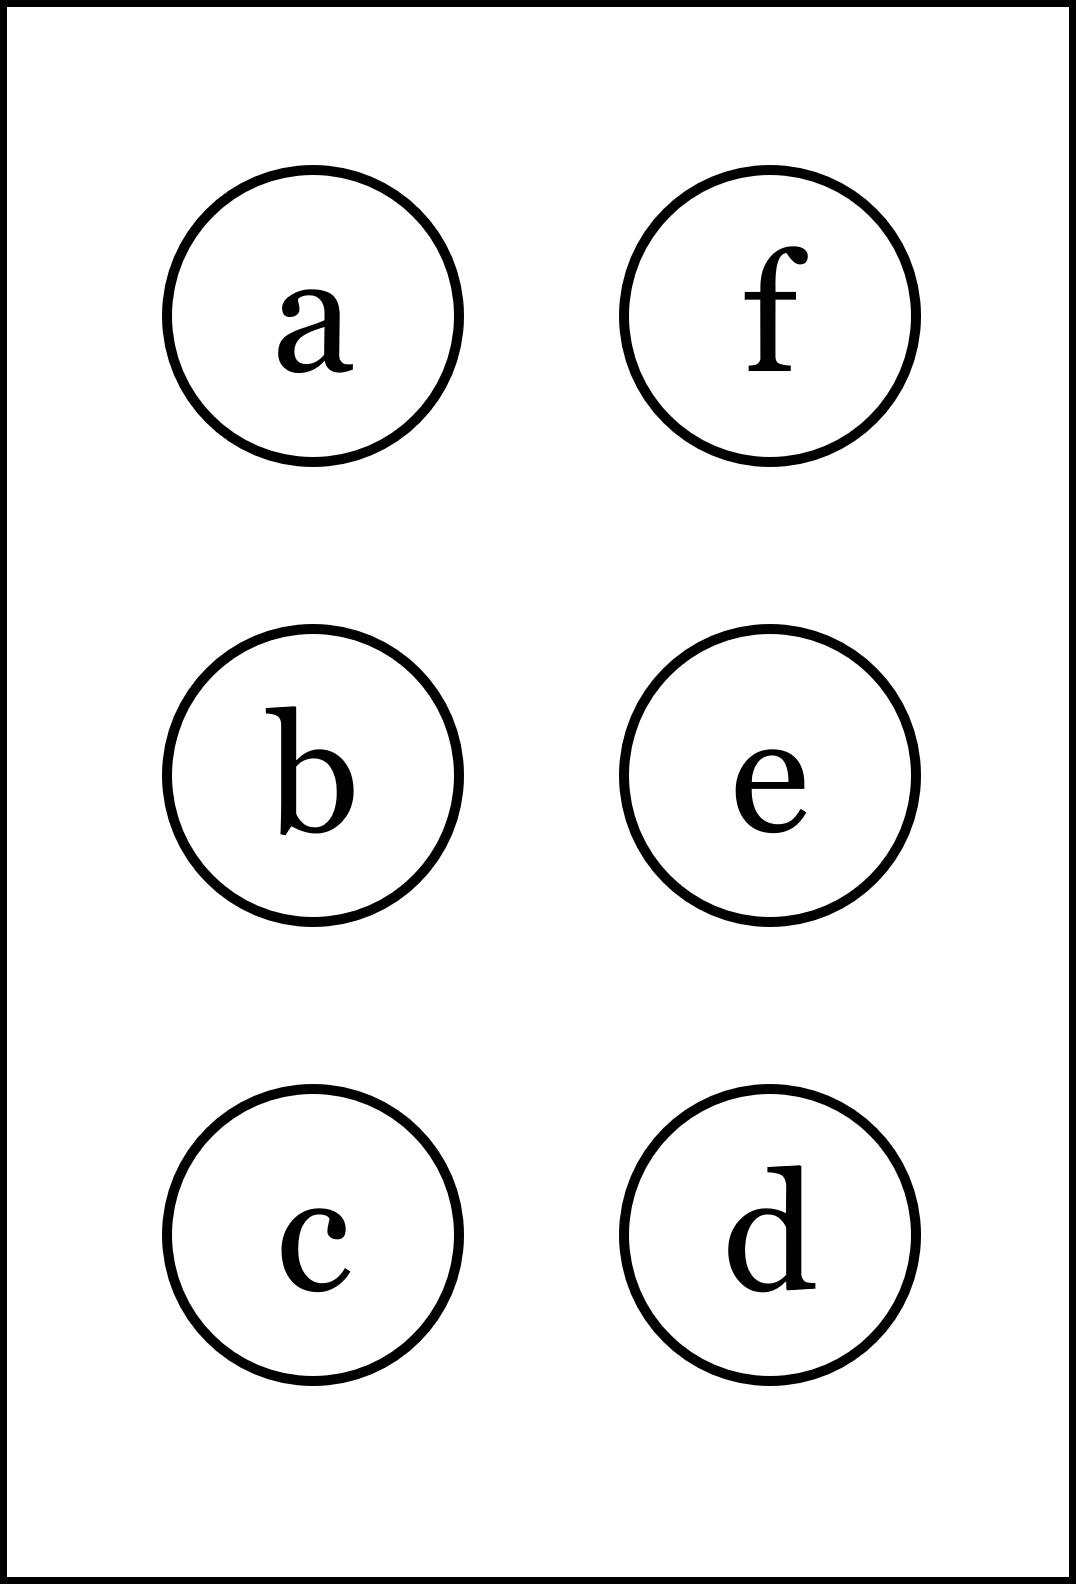
\includegraphics[height=40mm]{../images/braille.png}
{\small Písmeno Braillovej abecedy}
\end{center}
\end{minipage}
\end{center}
\end{minipage}
\\ \hdashline
\begin{minipage}[c][104.5mm][t]{0.5\linewidth}
\begin{center}
\vspace{7mm}
{\huge Viazané extrémy, skupina \textit{Gamma $\gamma$} -\romannumeral3}\\[5mm]
\textit{Jméno:}\phantom{xxxxxxxxxxxxxxxxxxxxxxxxxxxxxxxxxxxxxxxxxxxxxxxxxxxxxxxxxxxxxxxxx}\\[5mm]
\begin{minipage}{0.95\linewidth}
\begin{center}
Cílem je najít \textbf{vázané extrémy} funkce $f(x,y)$ zadané v \textbf{(a)} spolu s vazbou (podmínkou). Postupuj podle krokú v \textbf{(b)} až \textbf{(f)}. Pokud se medzivýsledky shodujú s těmi za otazníky,\\tak napravo obarvi příslušející kroužek načerno. \textbf{Spolu odevzdejte výsledné slovo}.
\end{center}
\end{minipage}
\\[1mm]
\begin{minipage}{0.79\linewidth}
\begin{center}
\begin{varwidth}{\linewidth}
\begin{enumerate}
\normalsize
\item $f(x,y)=-6x-8y+1 \enspace , \enspace \mathrm{vazba:} \enspace x^2+y^2=100$\quad \dotfill\; ???\;\dotfill \quad vybarvi
\item Sestav $L(\lambda,x,y)$ a spočti $\pdv{L}{x}=$\quad \dotfill\; ???\;\dotfill \quad $-6+\lambda x$
\item Takisto spočti $\pdv{L}{y}=$\quad \dotfill\; ???\;\dotfill \quad $+8+2\lambda y$
\item Z podmínek $\pdv{L}{x}=0 , \pdv{L}{y}=0$ vyjádři $x,y$ v závislosti na $\lambda$.\\ \phantom{xxxxxx}Následne $x,y$ dosaď do vazbové rovnice\\ \phantom{xxxxxx}a vypočti dva výsledky pro $\lambda$.\quad \dotfill\; ???\;\dotfill \quad $\lambda_1+\lambda_2=2$
\item Pomocou $\lambda$ urč dvě dvojice pro $x,y$.\quad \dotfill\; ???\;\dotfill \quad $x_1 x_2 y_1 y_2=2304$
\item Najdi funkční hodnoty pro oba vázané stacionární body\\ \phantom{xxxxxx}a vyber tu najvětší. $f_{\text{max}}(x,y)=$\quad \dotfill\; ???\;\dotfill \quad $100$
\end{enumerate}
\end{varwidth}
\end{center}
\end{minipage}
\begin{minipage}{0.20\linewidth}
\begin{center}
{\Huge\bfseries 3.} \\[2mm]
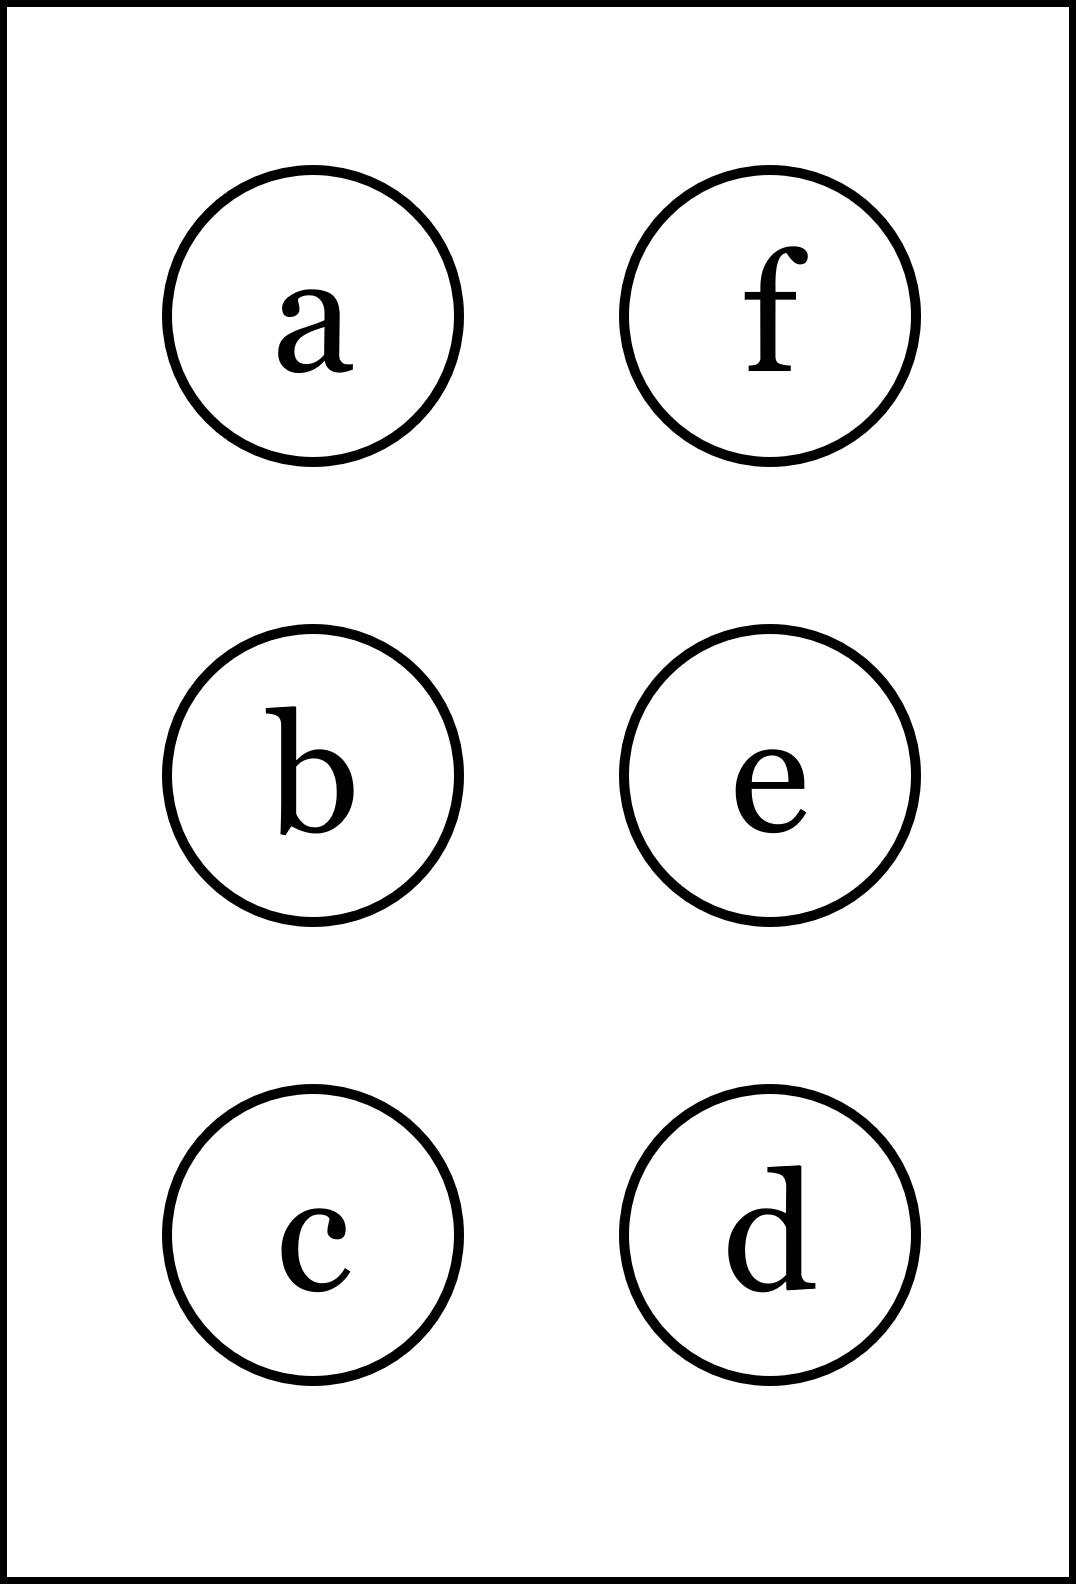
\includegraphics[height=40mm]{../images/braille.png}
{\small Písmeno Braillovej abecedy}
\end{center}
\end{minipage}
\end{center}
\end{minipage}
&
\begin{minipage}[c][104.5mm][t]{0.5\linewidth}
\begin{center}
\vspace{7mm}
{\huge Viazané extrémy, skupina \textit{Gamma $\gamma$} -\romannumeral4}\\[5mm]
\textit{Jméno:}\phantom{xxxxxxxxxxxxxxxxxxxxxxxxxxxxxxxxxxxxxxxxxxxxxxxxxxxxxxxxxxxxxxxxx}\\[5mm]
\begin{minipage}{0.95\linewidth}
\begin{center}
Cílem je najít \textbf{vázané extrémy} funkce $f(x,y)$ zadané v \textbf{(a)} spolu s vazbou (podmínkou). Postupuj podle krokú v \textbf{(b)} až \textbf{(f)}. Pokud se medzivýsledky shodujú s těmi za otazníky,\\tak napravo obarvi příslušející kroužek načerno. \textbf{Spolu odevzdejte výsledné slovo}.
\end{center}
\end{minipage}
\\[1mm]
\begin{minipage}{0.79\linewidth}
\begin{center}
\begin{varwidth}{\linewidth}
\begin{enumerate}
\normalsize
\item $f(x,y)=10x-24y-2 \enspace , \enspace \mathrm{vazba:} \enspace x^2+y^2=676$\quad \dotfill\; ???\;\dotfill \quad vybarvi
\item Sestav $L(\lambda,x,y)$ a spočti $\pdv{L}{x}=$\quad \dotfill\; ???\;\dotfill \quad $10+\lambda x$
\item Takisto spočti $\pdv{L}{y}=$\quad \dotfill\; ???\;\dotfill \quad $-24+2\lambda y$
\item Z podmínek $\pdv{L}{x}=0 , \pdv{L}{y}=0$ vyjádři $x,y$ v závislosti na $\lambda$.\\ \phantom{xxxxxx}Následne $x,y$ dosaď do vazbové rovnice\\ \phantom{xxxxxx}a vypočti dva výsledky pro $\lambda$.\quad \dotfill\; ???\;\dotfill \quad $\lambda_1+\lambda_2=-2$
\item Pomocou $\lambda$ urč dvě dvojice pro $x,y$.\quad \dotfill\; ???\;\dotfill \quad $x_1 x_2 y_1 y_2=-2400$
\item Najdi funkční hodnoty pro oba vázané stacionární body\\ \phantom{xxxxxx}a vyber tu najvětší. $f_{\text{max}}(x,y)=$\quad \dotfill\; ???\;\dotfill \quad $673$
\end{enumerate}
\end{varwidth}
\end{center}
\end{minipage}
\begin{minipage}{0.20\linewidth}
\begin{center}
{\Huge\bfseries 4.} \\[2mm]
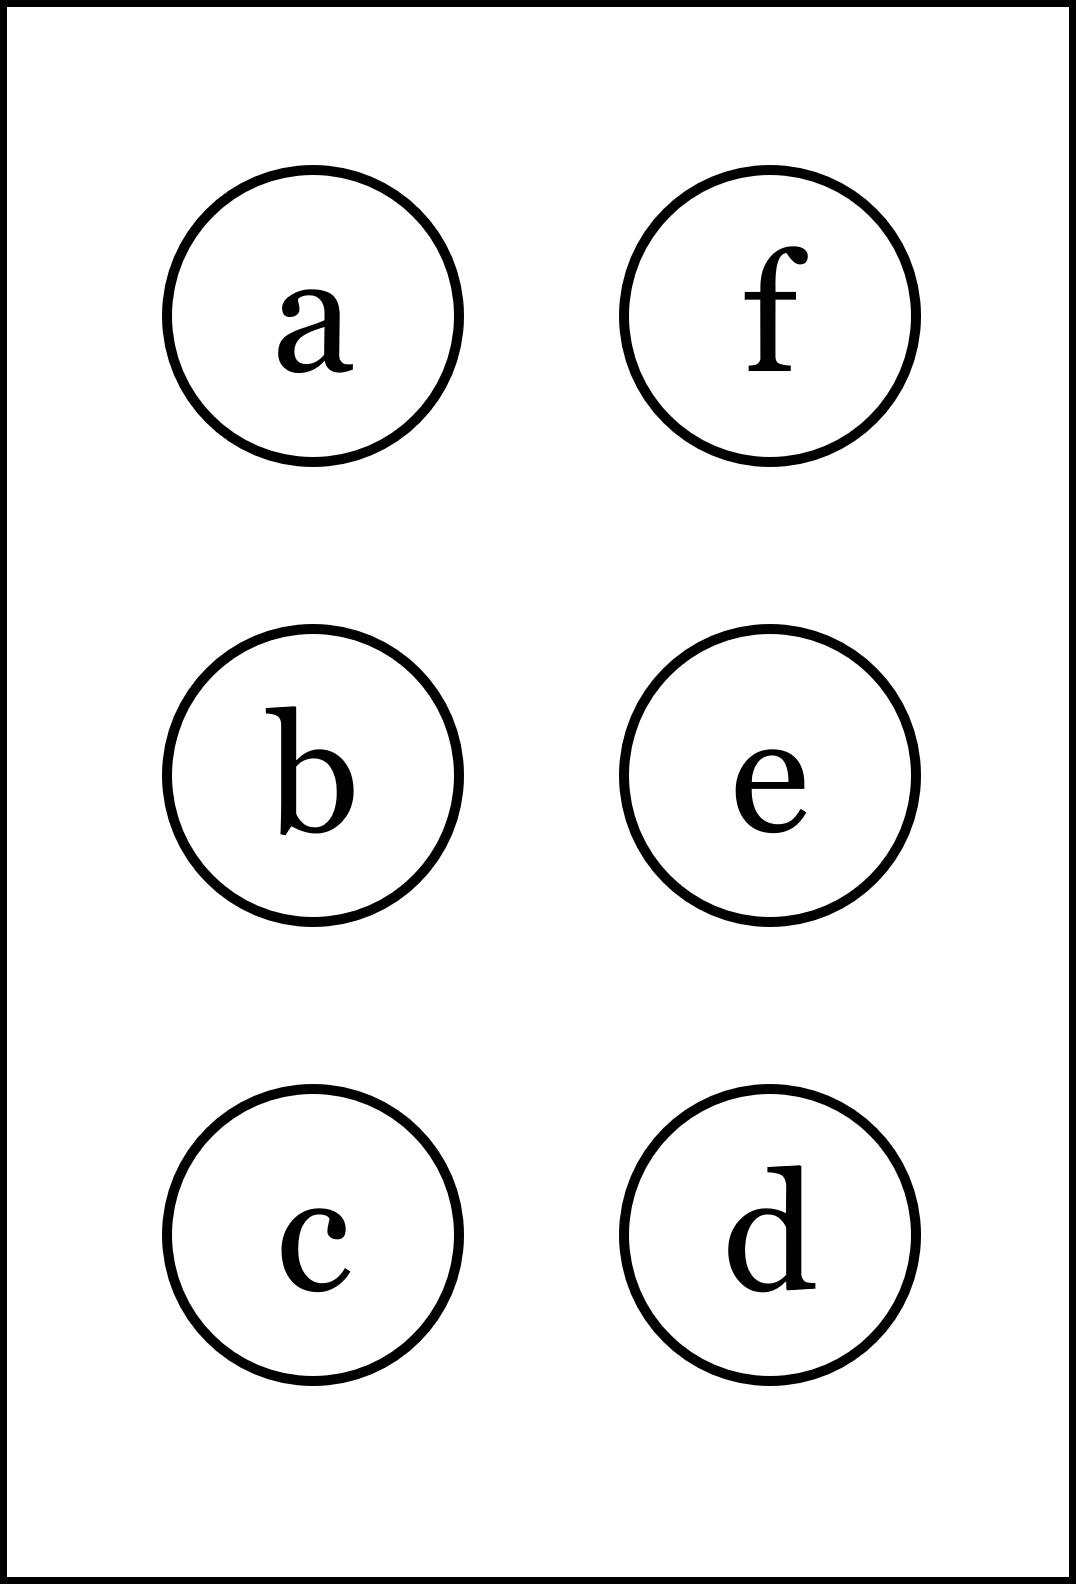
\includegraphics[height=40mm]{../images/braille.png}
{\small Písmeno Braillovej abecedy}
\end{center}
\end{minipage}
\end{center}
\end{minipage}
%
\end{tabular}
\newpage
\thispagestyle{empty}
\begin{tabular}{c:c}
\begin{minipage}[c][104.5mm][t]{0.5\linewidth}
\begin{center}
\vspace{7mm}
{\huge Viazané extrémy, skupina \textit{Delta $\delta$} -\romannumeral1}\\[5mm]
\textit{Jméno:}\phantom{xxxxxxxxxxxxxxxxxxxxxxxxxxxxxxxxxxxxxxxxxxxxxxxxxxxxxxxxxxxxxxxxx}\\[5mm]
\begin{minipage}{0.95\linewidth}
\begin{center}
Cílem je najít \textbf{vázané extrémy} funkce $f(x,y)$ zadané v \textbf{(a)} spolu s vazbou (podmínkou). Postupuj podle krokú v \textbf{(b)} až \textbf{(f)}. Pokud se medzivýsledky shodujú s těmi za otazníky,\\tak napravo obarvi příslušející kroužek načerno. \textbf{Spolu odevzdejte výsledné slovo}.
\end{center}
\end{minipage}
\\[1mm]
\begin{minipage}{0.79\linewidth}
\begin{center}
\begin{varwidth}{\linewidth}
\begin{enumerate}
\normalsize
\item $f(x,y)=3x+4y+6 \enspace , \enspace \mathrm{vazba:} \enspace x^2+y^2=25$\quad \dotfill\; ???\;\dotfill \quad vybarvi
\item Sestav $L(\lambda,x,y)$ a spočti $\pdv{L}{x}=$\quad \dotfill\; ???\;\dotfill \quad $3+2\lambda x$
\item Takisto spočti $\pdv{L}{y}=$\quad \dotfill\; ???\;\dotfill \quad $4+2\lambda y$
\item Z podmínek $\pdv{L}{x}=0 , \pdv{L}{y}=0$ vyjádři $x,y$ v závislosti na $\lambda$.\\ \phantom{xxxxxx}Následne $x,y$ dosaď do vazbové rovnice\\ \phantom{xxxxxx}a vypočti dva výsledky pro $\lambda$.\quad \dotfill\; ???\;\dotfill \quad $\lambda_1+\lambda_2=2$
\item Pomocou $\lambda$ urč dvě dvojice pro $x,y$.\quad \dotfill\; ???\;\dotfill \quad $x_1 x_2 y_1 y_2=144$
\item Najdi funkční hodnoty pro oba vázané stacionární body\\ \phantom{xxxxxx}a vyber tu najvětší. $f_{\text{max}}(x,y)=$\quad \dotfill\; ???\;\dotfill \quad $30$
\end{enumerate}
\end{varwidth}
\end{center}
\end{minipage}
\begin{minipage}{0.20\linewidth}
\begin{center}
{\Huge\bfseries 1.} \\[2mm]
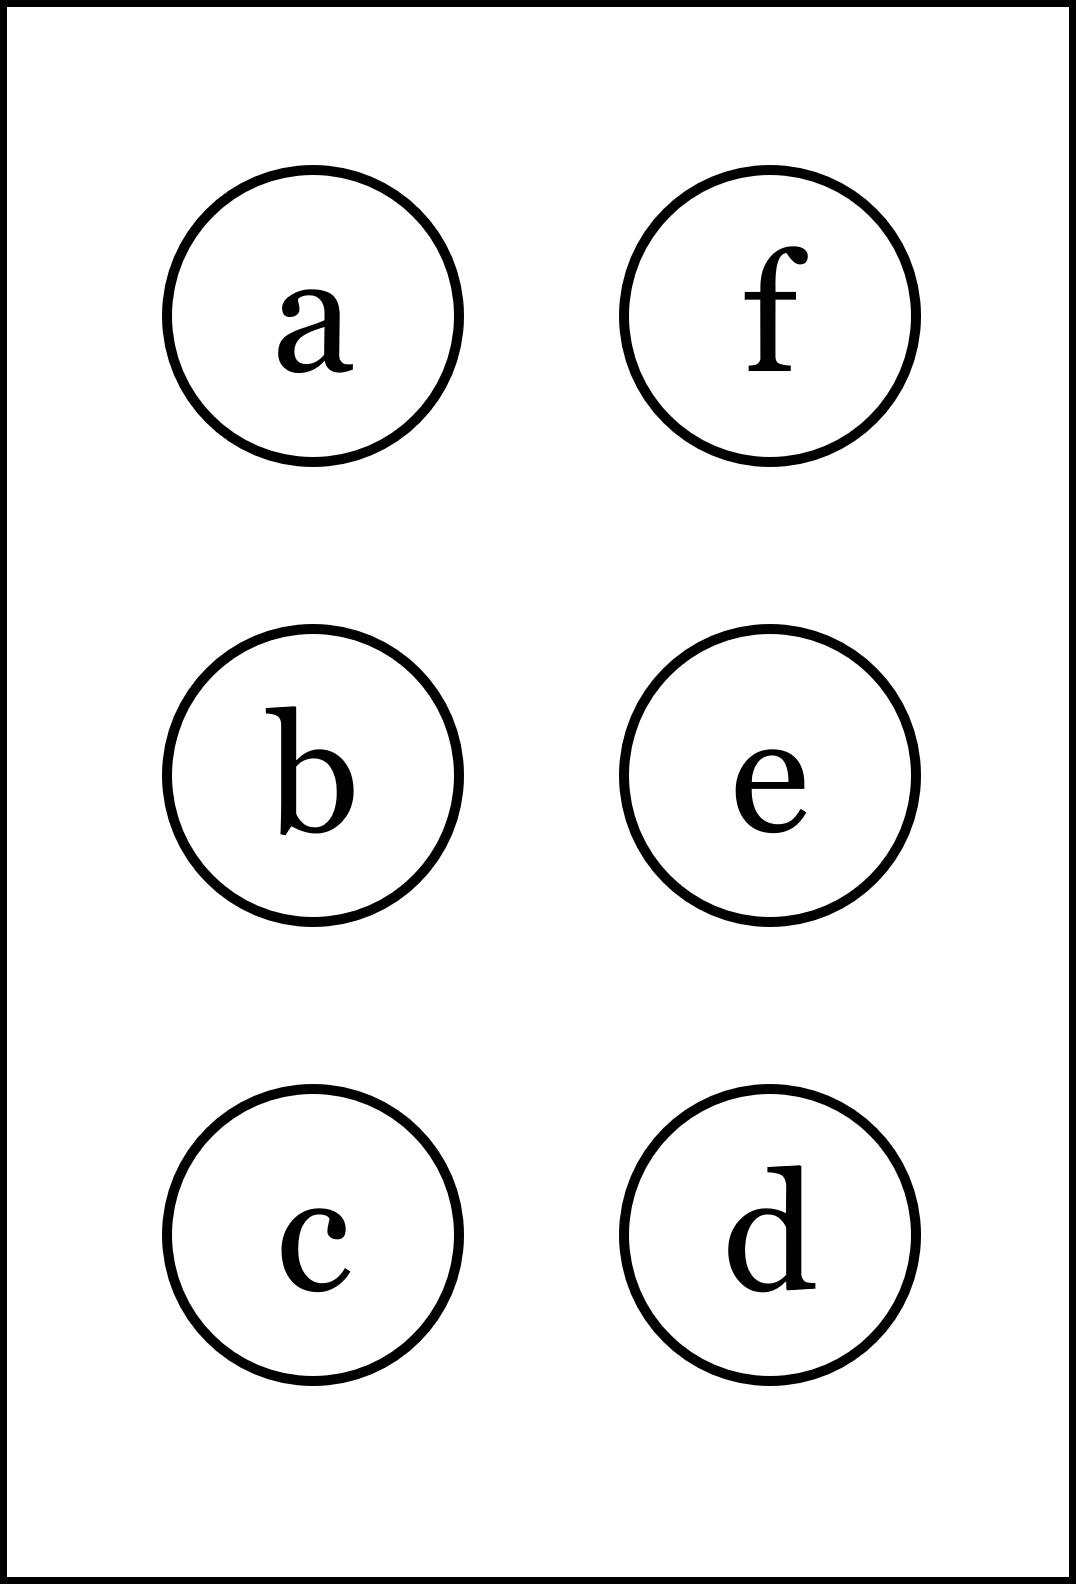
\includegraphics[height=40mm]{../images/braille.png}
{\small Písmeno Braillovej abecedy}
\end{center}
\end{minipage}
\end{center}
\end{minipage}
&
\begin{minipage}[c][104.5mm][t]{0.5\linewidth}
\begin{center}
\vspace{7mm}
{\huge Viazané extrémy, skupina \textit{Delta $\delta$} -\romannumeral2}\\[5mm]
\textit{Jméno:}\phantom{xxxxxxxxxxxxxxxxxxxxxxxxxxxxxxxxxxxxxxxxxxxxxxxxxxxxxxxxxxxxxxxxx}\\[5mm]
\begin{minipage}{0.95\linewidth}
\begin{center}
Cílem je najít \textbf{vázané extrémy} funkce $f(x,y)$ zadané v \textbf{(a)} spolu s vazbou (podmínkou). Postupuj podle krokú v \textbf{(b)} až \textbf{(f)}. Pokud se medzivýsledky shodujú s těmi za otazníky,\\tak napravo obarvi příslušející kroužek načerno. \textbf{Spolu odevzdejte výsledné slovo}.
\end{center}
\end{minipage}
\\[1mm]
\begin{minipage}{0.79\linewidth}
\begin{center}
\begin{varwidth}{\linewidth}
\begin{enumerate}
\normalsize
\item $f(x,y)=-5x+12y-2 \enspace , \enspace \mathrm{vazba:} \enspace x^2+y^2=169$\quad \dotfill\; ???\;\dotfill \quad vybarvi
\item Sestav $L(\lambda,x,y)$ a spočti $\pdv{L}{x}=$\quad \dotfill\; ???\;\dotfill \quad $-5+\lambda x$
\item Takisto spočti $\pdv{L}{y}=$\quad \dotfill\; ???\;\dotfill \quad $-12+2\lambda y$
\item Z podmínek $\pdv{L}{x}=0 , \pdv{L}{y}=0$ vyjádři $x,y$ v závislosti na $\lambda$.\\ \phantom{xxxxxx}Následne $x,y$ dosaď do vazbové rovnice\\ \phantom{xxxxxx}a vypočti dva výsledky pro $\lambda$.\quad \dotfill\; ???\;\dotfill \quad $\lambda_1+\lambda_2=1$
\item Pomocou $\lambda$ urč dvě dvojice pro $x,y$.\quad \dotfill\; ???\;\dotfill \quad $x_1 x_2 y_1 y_2=300$
\item Najdi funkční hodnoty pro oba vázané stacionární body\\ \phantom{xxxxxx}a vyber tu najvětší. $f_{\text{max}}(x,y)=$\quad \dotfill\; ???\;\dotfill \quad $166$
\end{enumerate}
\end{varwidth}
\end{center}
\end{minipage}
\begin{minipage}{0.20\linewidth}
\begin{center}
{\Huge\bfseries 2.} \\[2mm]
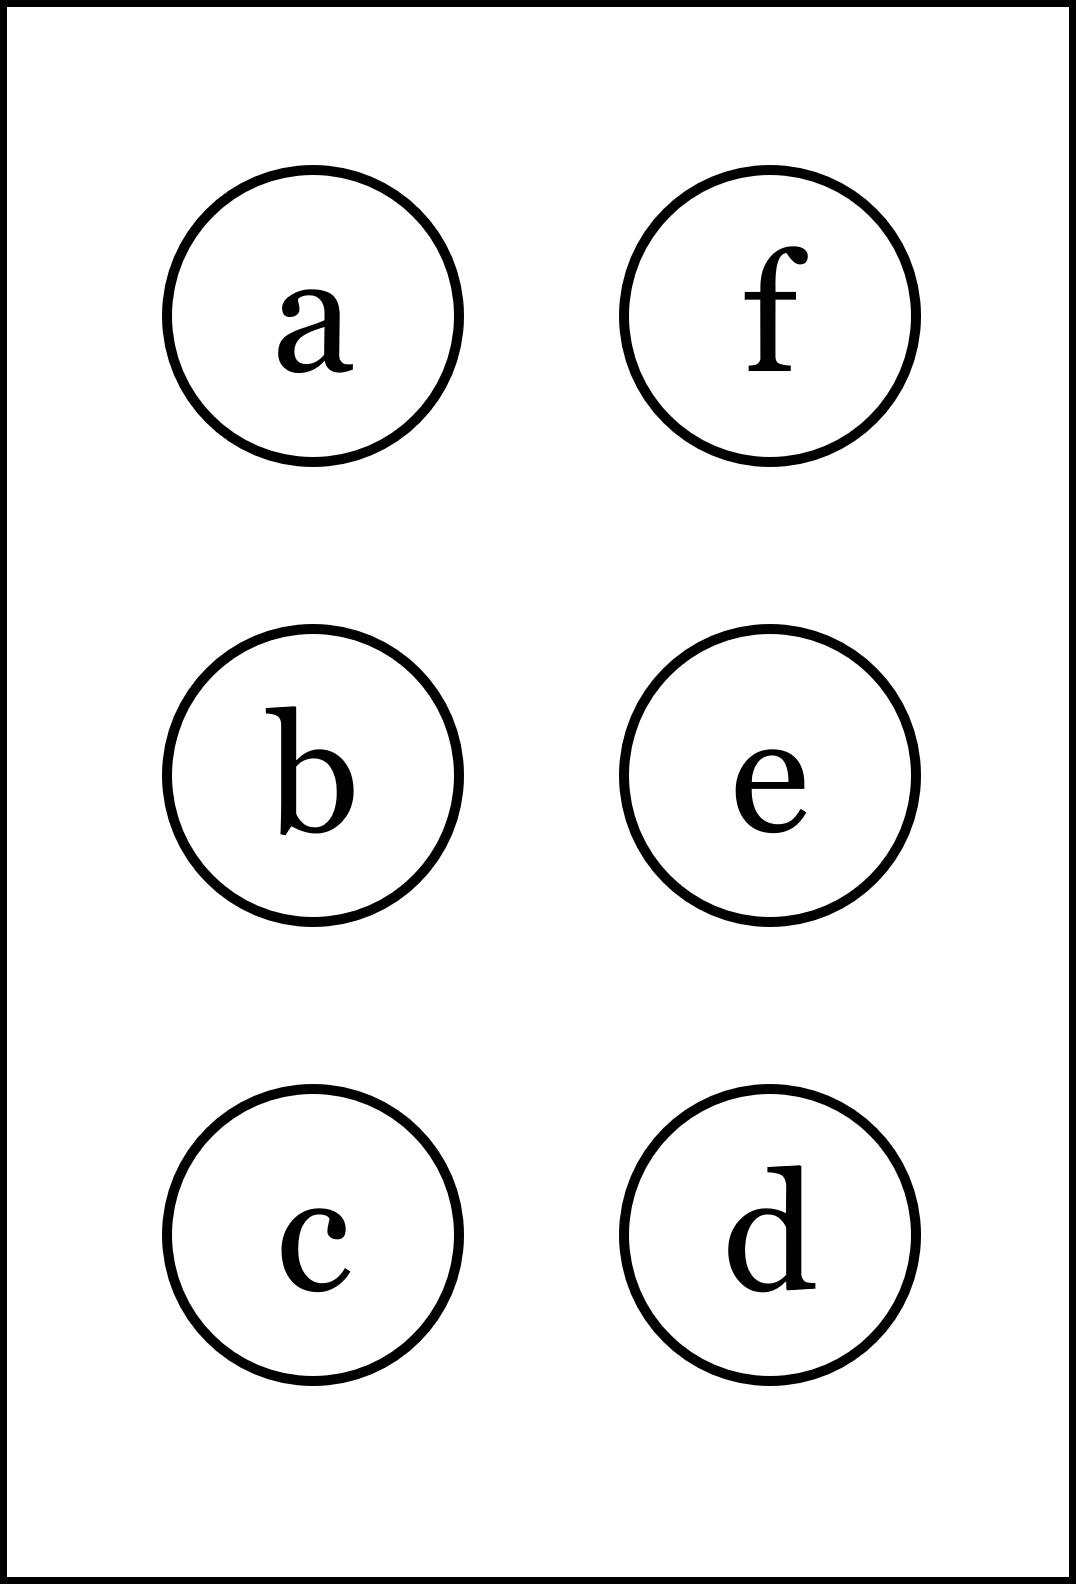
\includegraphics[height=40mm]{../images/braille.png}
{\small Písmeno Braillovej abecedy}
\end{center}
\end{minipage}
\end{center}
\end{minipage}
\\ \hdashline
\begin{minipage}[c][104.5mm][t]{0.5\linewidth}
\begin{center}
\vspace{7mm}
{\huge Viazané extrémy, skupina \textit{Delta $\delta$} -\romannumeral3}\\[5mm]
\textit{Jméno:}\phantom{xxxxxxxxxxxxxxxxxxxxxxxxxxxxxxxxxxxxxxxxxxxxxxxxxxxxxxxxxxxxxxxxx}\\[5mm]
\begin{minipage}{0.95\linewidth}
\begin{center}
Cílem je najít \textbf{vázané extrémy} funkce $f(x,y)$ zadané v \textbf{(a)} spolu s vazbou (podmínkou). Postupuj podle krokú v \textbf{(b)} až \textbf{(f)}. Pokud se medzivýsledky shodujú s těmi za otazníky,\\tak napravo obarvi příslušející kroužek načerno. \textbf{Spolu odevzdejte výsledné slovo}.
\end{center}
\end{minipage}
\\[1mm]
\begin{minipage}{0.79\linewidth}
\begin{center}
\begin{varwidth}{\linewidth}
\begin{enumerate}
\normalsize
\item $f(x,y)=6x+8y+7 \enspace , \enspace \mathrm{vazba:} \enspace x^2+y^2=100$\quad \dotfill\; ???\;\dotfill \quad vybarvi
\item Sestav $L(\lambda,x,y)$ a spočti $\pdv{L}{x}=$\quad \dotfill\; ???\;\dotfill \quad $6+\lambda x$
\item Takisto spočti $\pdv{L}{y}=$\quad \dotfill\; ???\;\dotfill \quad $-8+2\lambda y$
\item Z podmínek $\pdv{L}{x}=0 , \pdv{L}{y}=0$ vyjádři $x,y$ v závislosti na $\lambda$.\\ \phantom{xxxxxx}Následne $x,y$ dosaď do vazbové rovnice\\ \phantom{xxxxxx}a vypočti dva výsledky pro $\lambda$.\quad \dotfill\; ???\;\dotfill \quad $\lambda_1+\lambda_2=1$
\item Pomocou $\lambda$ urč dvě dvojice pro $x,y$.\quad \dotfill\; ???\;\dotfill \quad $x_1 x_2 y_1 y_2=2304$
\item Najdi funkční hodnoty pro oba vázané stacionární body\\ \phantom{xxxxxx}a vyber tu najvětší. $f_{\text{max}}(x,y)=$\quad \dotfill\; ???\;\dotfill \quad $107$
\end{enumerate}
\end{varwidth}
\end{center}
\end{minipage}
\begin{minipage}{0.20\linewidth}
\begin{center}
{\Huge\bfseries 3.} \\[2mm]
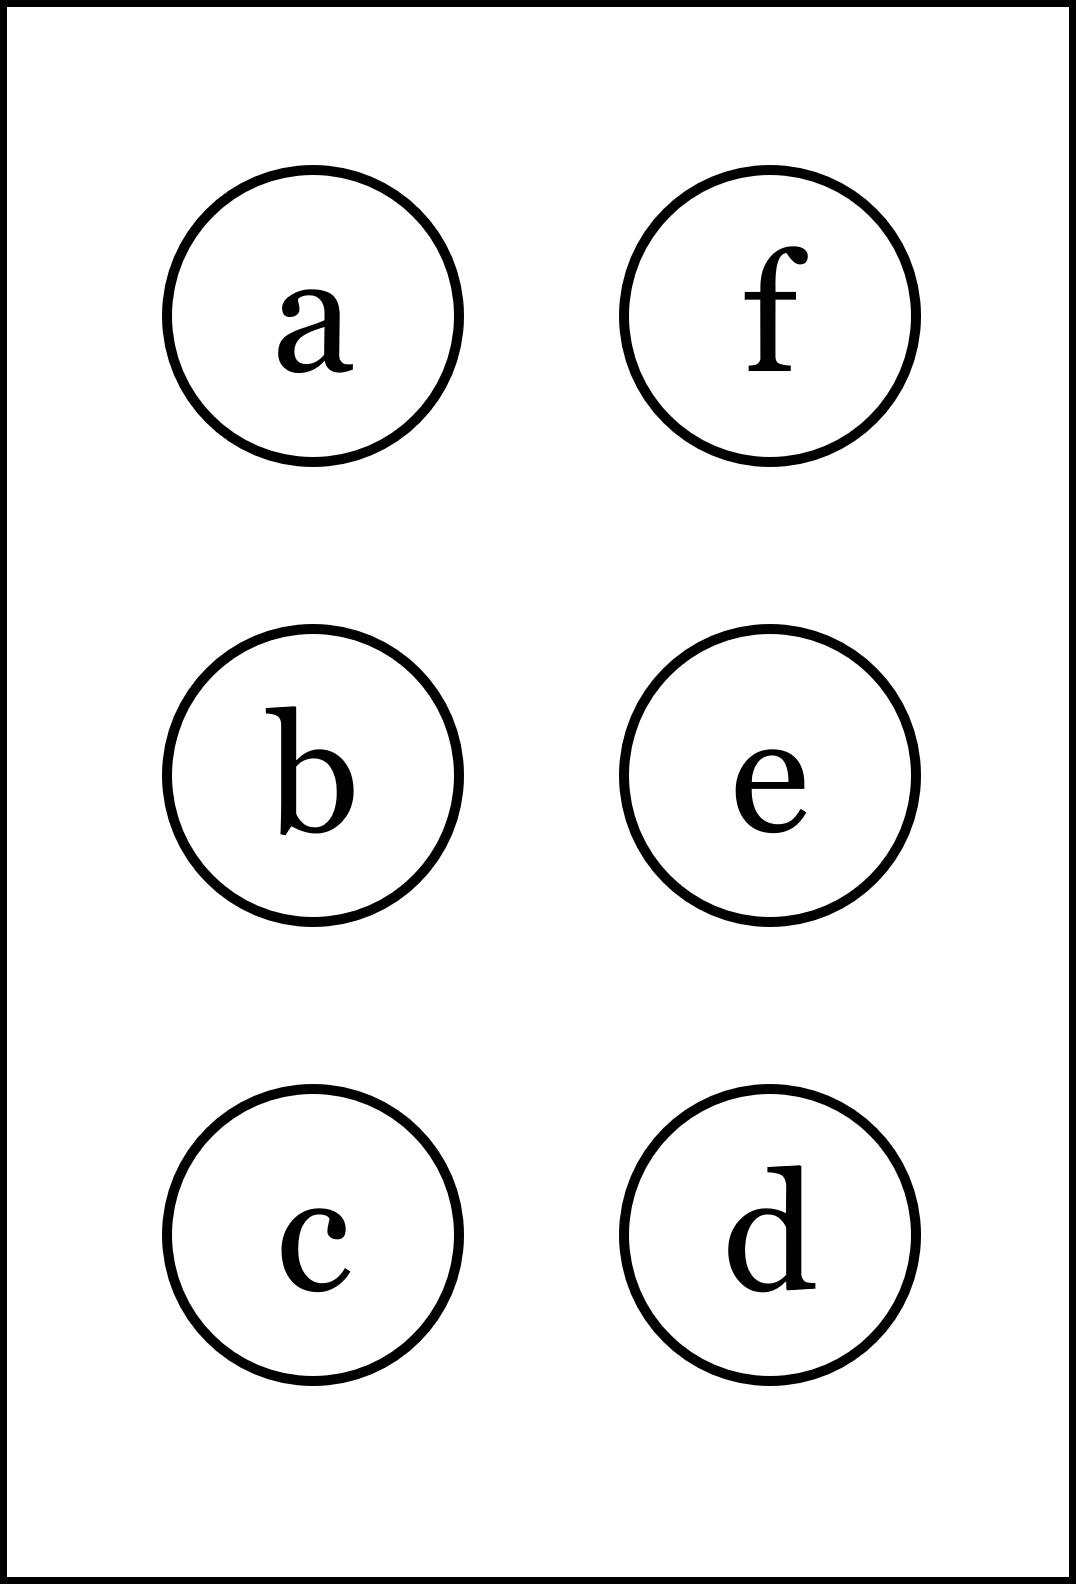
\includegraphics[height=40mm]{../images/braille.png}
{\small Písmeno Braillovej abecedy}
\end{center}
\end{minipage}
\end{center}
\end{minipage}
&
\begin{minipage}[c][104.5mm][t]{0.5\linewidth}
\begin{center}
\vspace{7mm}
{\huge Viazané extrémy, skupina \textit{Delta $\delta$} -\romannumeral4}\\[5mm]
\textit{Jméno:}\phantom{xxxxxxxxxxxxxxxxxxxxxxxxxxxxxxxxxxxxxxxxxxxxxxxxxxxxxxxxxxxxxxxxx}\\[5mm]
\begin{minipage}{0.95\linewidth}
\begin{center}
Cílem je najít \textbf{vázané extrémy} funkce $f(x,y)$ zadané v \textbf{(a)} spolu s vazbou (podmínkou). Postupuj podle krokú v \textbf{(b)} až \textbf{(f)}. Pokud se medzivýsledky shodujú s těmi za otazníky,\\tak napravo obarvi příslušející kroužek načerno. \textbf{Spolu odevzdejte výsledné slovo}.
\end{center}
\end{minipage}
\\[1mm]
\begin{minipage}{0.79\linewidth}
\begin{center}
\begin{varwidth}{\linewidth}
\begin{enumerate}
\normalsize
\item $f(x,y)=10x+24y+6 \enspace , \enspace \mathrm{vazba:} \enspace x^2+y^2=676$\quad \dotfill\; ???\;\dotfill \quad vybarvi
\item Sestav $L(\lambda,x,y)$ a spočti $\pdv{L}{x}=$\quad \dotfill\; ???\;\dotfill \quad $10+\lambda x$
\item Takisto spočti $\pdv{L}{y}=$\quad \dotfill\; ???\;\dotfill \quad $-24+2\lambda y$
\item Z podmínek $\pdv{L}{x}=0 , \pdv{L}{y}=0$ vyjádři $x,y$ v závislosti na $\lambda$.\\ \phantom{xxxxxx}Následne $x,y$ dosaď do vazbové rovnice\\ \phantom{xxxxxx}a vypočti dva výsledky pro $\lambda$.\quad \dotfill\; ???\;\dotfill \quad $\lambda_1+\lambda_2=1$
\item Pomocou $\lambda$ urč dvě dvojice pro $x,y$.\quad \dotfill\; ???\;\dotfill \quad $x_1 x_2 y_1 y_2=2400$
\item Najdi funkční hodnoty pro oba vázané stacionární body\\ \phantom{xxxxxx}a vyber tu najvětší. $f_{\text{max}}(x,y)=$\quad \dotfill\; ???\;\dotfill \quad $681$
\end{enumerate}
\end{varwidth}
\end{center}
\end{minipage}
\begin{minipage}{0.20\linewidth}
\begin{center}
{\Huge\bfseries 4.} \\[2mm]
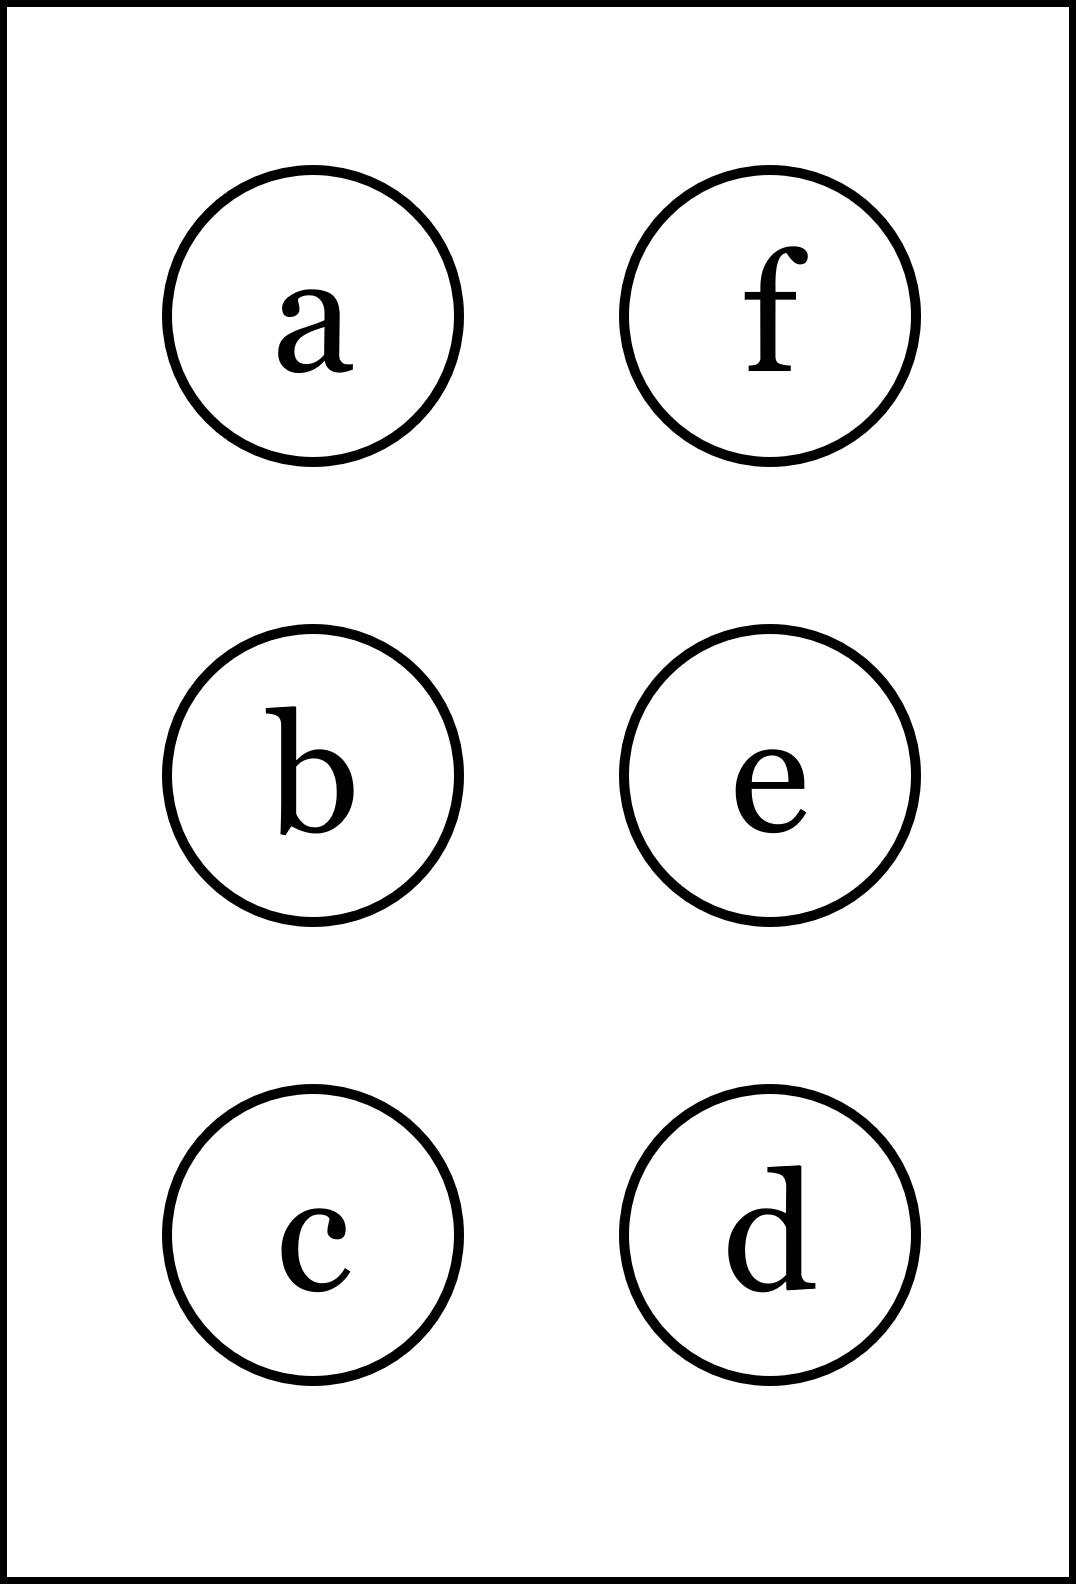
\includegraphics[height=40mm]{../images/braille.png}
{\small Písmeno Braillovej abecedy}
\end{center}
\end{minipage}
\end{center}
\end{minipage}
%
\end{tabular}
\newpage
\thispagestyle{empty}
\begin{tabular}{c:c}
\begin{minipage}[c][104.5mm][t]{0.5\linewidth}
\begin{center}
\vspace{7mm}
{\huge Viazané extrémy, skupina \textit{Epsilon $\epsilon$} -\romannumeral1}\\[5mm]
\textit{Jméno:}\phantom{xxxxxxxxxxxxxxxxxxxxxxxxxxxxxxxxxxxxxxxxxxxxxxxxxxxxxxxxxxxxxxxxx}\\[5mm]
\begin{minipage}{0.95\linewidth}
\begin{center}
Cílem je najít \textbf{vázané extrémy} funkce $f(x,y)$ zadané v \textbf{(a)} spolu s vazbou (podmínkou). Postupuj podle krokú v \textbf{(b)} až \textbf{(f)}. Pokud se medzivýsledky shodujú s těmi za otazníky,\\tak napravo obarvi příslušející kroužek načerno. \textbf{Spolu odevzdejte výsledné slovo}.
\end{center}
\end{minipage}
\\[1mm]
\begin{minipage}{0.79\linewidth}
\begin{center}
\begin{varwidth}{\linewidth}
\begin{enumerate}
\normalsize
\item $f(x,y)=-3x+4y-3 \enspace , \enspace \mathrm{vazba:} \enspace x^2+y^2=25$\quad \dotfill\; ???\;\dotfill \quad vybarvi
\item Sestav $L(\lambda,x,y)$ a spočti $\pdv{L}{x}=$\quad \dotfill\; ???\;\dotfill \quad $-3+\lambda x$
\item Takisto spočti $\pdv{L}{y}=$\quad \dotfill\; ???\;\dotfill \quad $4+2\lambda y$
\item Z podmínek $\pdv{L}{x}=0 , \pdv{L}{y}=0$ vyjádři $x,y$ v závislosti na $\lambda$.\\ \phantom{xxxxxx}Následne $x,y$ dosaď do vazbové rovnice\\ \phantom{xxxxxx}a vypočti dva výsledky pro $\lambda$.\quad \dotfill\; ???\;\dotfill \quad $\lambda_1+\lambda_2=-2$
\item Pomocou $\lambda$ urč dvě dvojice pro $x,y$.\quad \dotfill\; ???\;\dotfill \quad $x_1 x_2 y_1 y_2=36$
\item Najdi funkční hodnoty pro oba vázané stacionární body\\ \phantom{xxxxxx}a vyber tu najvětší. $f_{\text{max}}(x,y)=$\quad \dotfill\; ???\;\dotfill \quad $21$
\end{enumerate}
\end{varwidth}
\end{center}
\end{minipage}
\begin{minipage}{0.20\linewidth}
\begin{center}
{\Huge\bfseries 1.} \\[2mm]
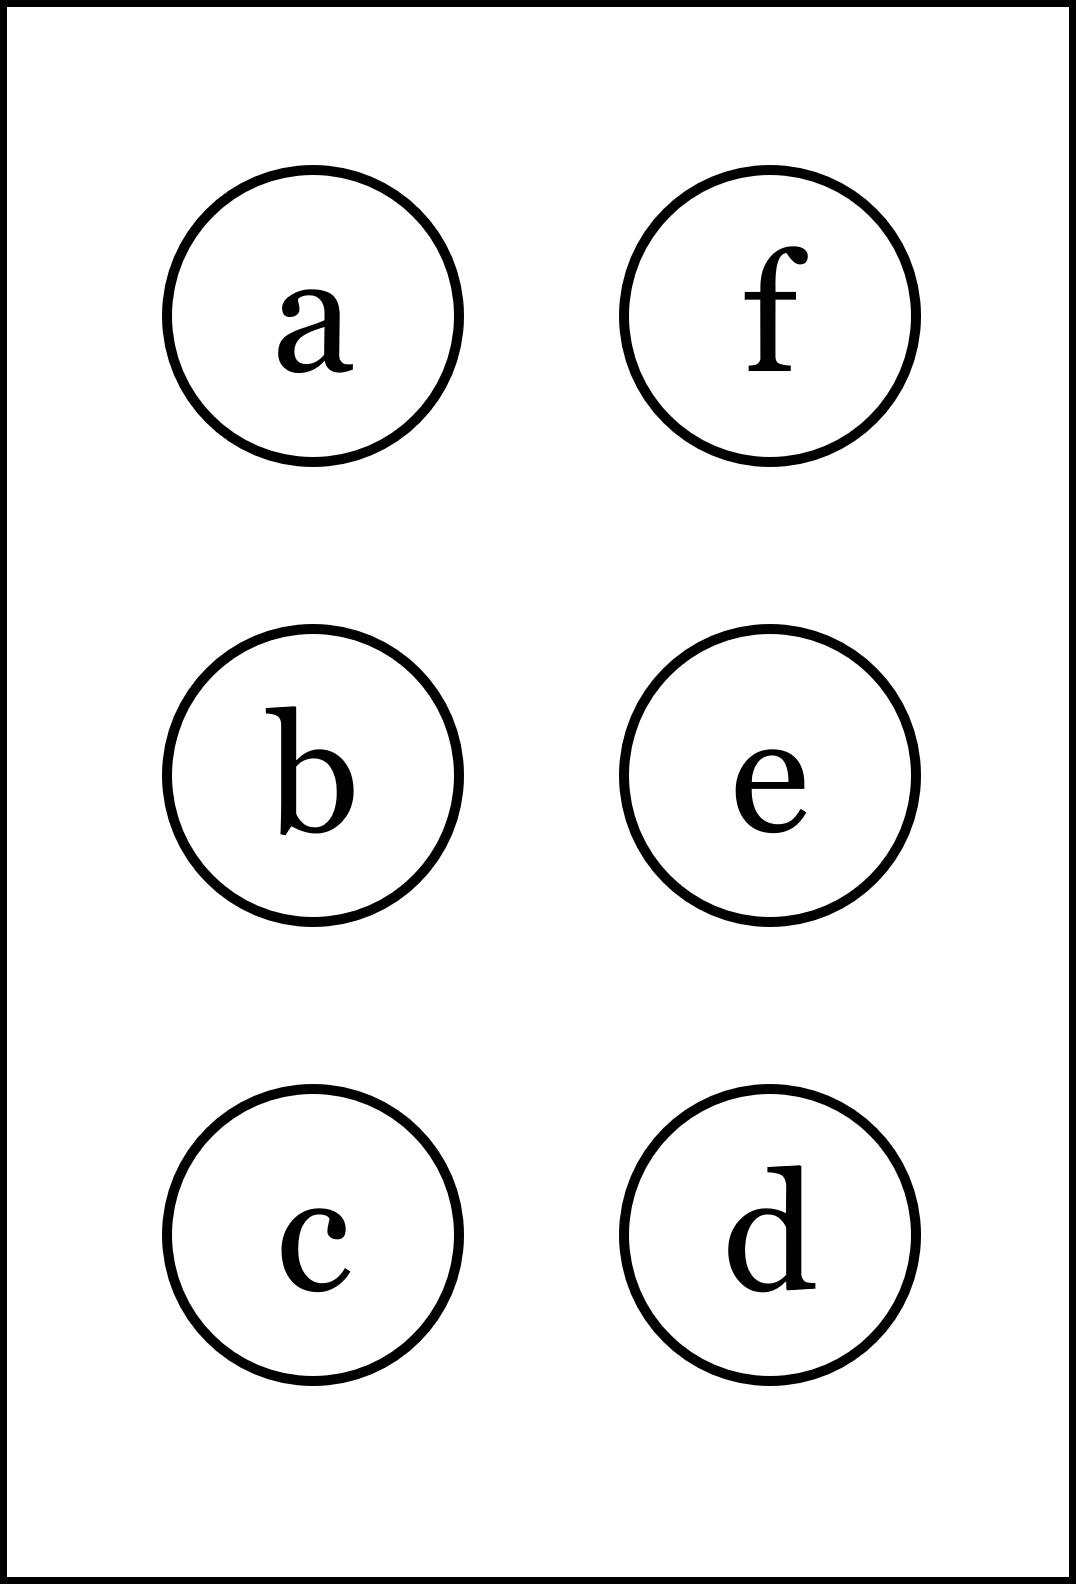
\includegraphics[height=40mm]{../images/braille.png}
{\small Písmeno Braillovej abecedy}
\end{center}
\end{minipage}
\end{center}
\end{minipage}
&
\begin{minipage}[c][104.5mm][t]{0.5\linewidth}
\begin{center}
\vspace{7mm}
{\huge Viazané extrémy, skupina \textit{Epsilon $\epsilon$} -\romannumeral2}\\[5mm]
\textit{Jméno:}\phantom{xxxxxxxxxxxxxxxxxxxxxxxxxxxxxxxxxxxxxxxxxxxxxxxxxxxxxxxxxxxxxxxxx}\\[5mm]
\begin{minipage}{0.95\linewidth}
\begin{center}
Cílem je najít \textbf{vázané extrémy} funkce $f(x,y)$ zadané v \textbf{(a)} spolu s vazbou (podmínkou). Postupuj podle krokú v \textbf{(b)} až \textbf{(f)}. Pokud se medzivýsledky shodujú s těmi za otazníky,\\tak napravo obarvi příslušející kroužek načerno. \textbf{Spolu odevzdejte výsledné slovo}.
\end{center}
\end{minipage}
\\[1mm]
\begin{minipage}{0.79\linewidth}
\begin{center}
\begin{varwidth}{\linewidth}
\begin{enumerate}
\normalsize
\item $f(x,y)=-5x-12y+1 \enspace , \enspace \mathrm{vazba:} \enspace x^2+y^2=169$\quad \dotfill\; ???\;\dotfill \quad vybarvi
\item Sestav $L(\lambda,x,y)$ a spočti $\pdv{L}{x}=$\quad \dotfill\; ???\;\dotfill \quad $-5+\lambda x$
\item Takisto spočti $\pdv{L}{y}=$\quad \dotfill\; ???\;\dotfill \quad $-12+2\lambda y$
\item Z podmínek $\pdv{L}{x}=0 , \pdv{L}{y}=0$ vyjádři $x,y$ v závislosti na $\lambda$.\\ \phantom{xxxxxx}Následne $x,y$ dosaď do vazbové rovnice\\ \phantom{xxxxxx}a vypočti dva výsledky pro $\lambda$.\quad \dotfill\; ???\;\dotfill \quad $\lambda_1+\lambda_2=-2$
\item Pomocou $\lambda$ urč dvě dvojice pro $x,y$.\quad \dotfill\; ???\;\dotfill \quad $x_1 x_2 y_1 y_2=3600$
\item Najdi funkční hodnoty pro oba vázané stacionární body\\ \phantom{xxxxxx}a vyber tu najvětší. $f_{\text{max}}(x,y)=$\quad \dotfill\; ???\;\dotfill \quad $169$
\end{enumerate}
\end{varwidth}
\end{center}
\end{minipage}
\begin{minipage}{0.20\linewidth}
\begin{center}
{\Huge\bfseries 2.} \\[2mm]
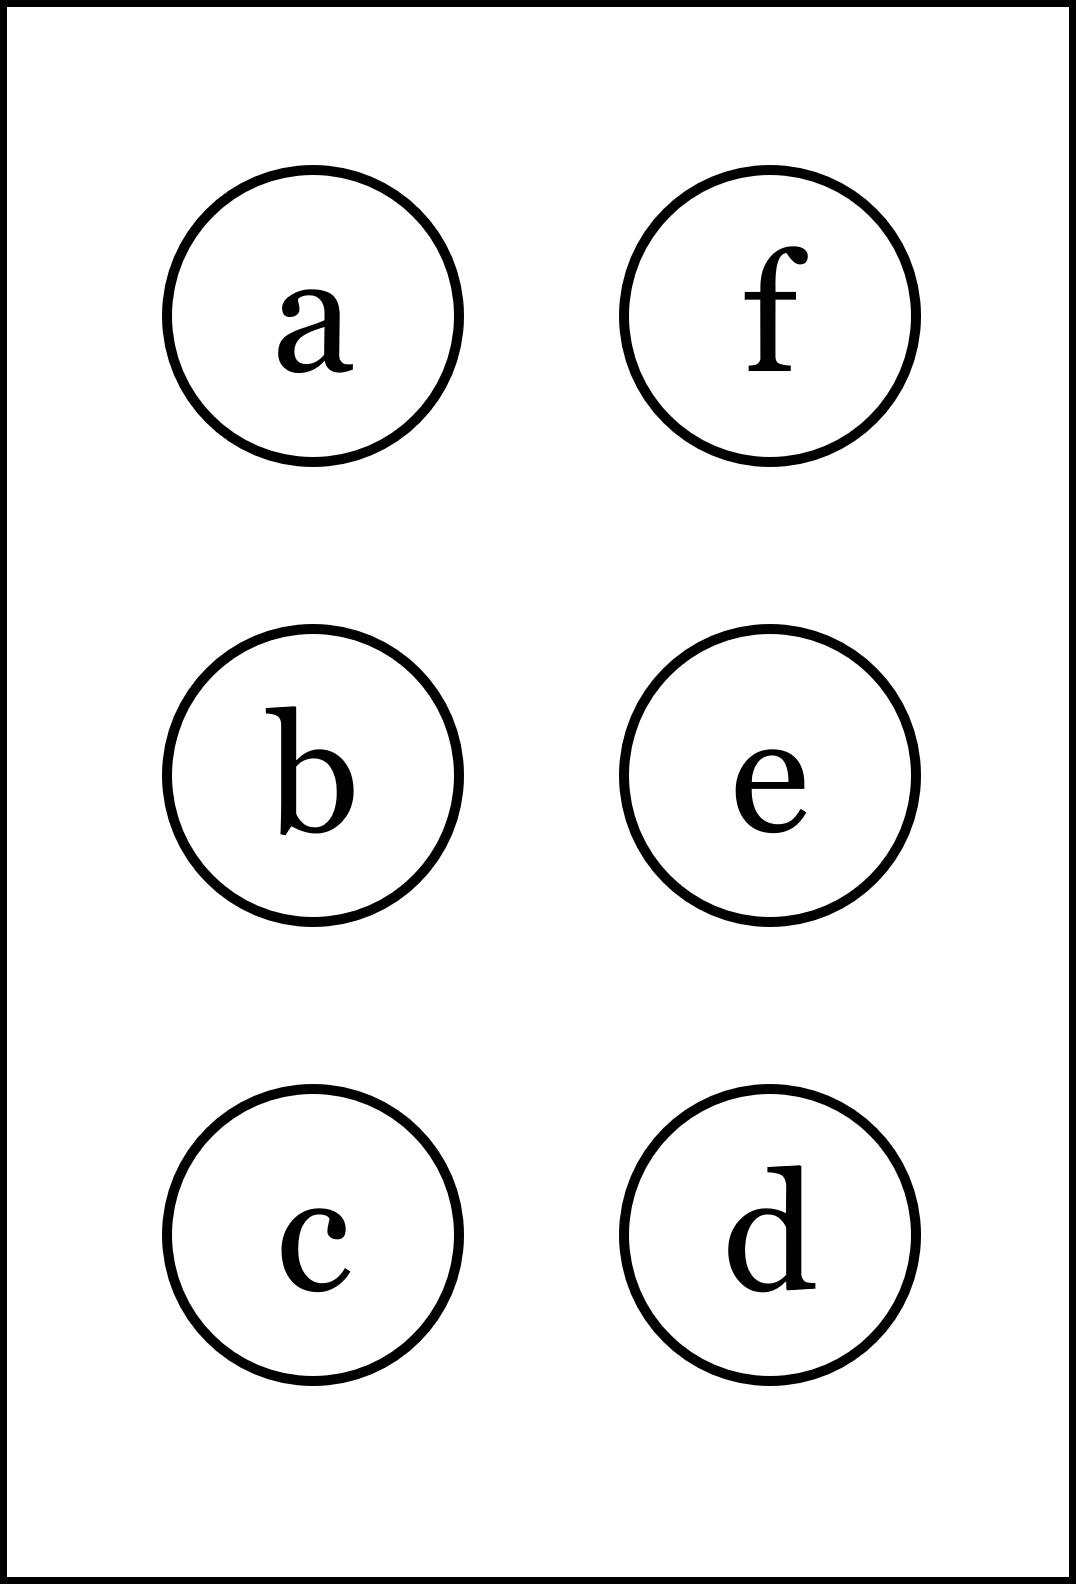
\includegraphics[height=40mm]{../images/braille.png}
{\small Písmeno Braillovej abecedy}
\end{center}
\end{minipage}
\end{center}
\end{minipage}
\\ \hdashline
\begin{minipage}[c][104.5mm][t]{0.5\linewidth}
\begin{center}
\vspace{7mm}
{\huge Viazané extrémy, skupina \textit{Epsilon $\epsilon$} -\romannumeral3}\\[5mm]
\textit{Jméno:}\phantom{xxxxxxxxxxxxxxxxxxxxxxxxxxxxxxxxxxxxxxxxxxxxxxxxxxxxxxxxxxxxxxxxx}\\[5mm]
\begin{minipage}{0.95\linewidth}
\begin{center}
Cílem je najít \textbf{vázané extrémy} funkce $f(x,y)$ zadané v \textbf{(a)} spolu s vazbou (podmínkou). Postupuj podle krokú v \textbf{(b)} až \textbf{(f)}. Pokud se medzivýsledky shodujú s těmi za otazníky,\\tak napravo obarvi příslušející kroužek načerno. \textbf{Spolu odevzdejte výsledné slovo}.
\end{center}
\end{minipage}
\\[1mm]
\begin{minipage}{0.79\linewidth}
\begin{center}
\begin{varwidth}{\linewidth}
\begin{enumerate}
\normalsize
\item $f(x,y)=6x-8y-2 \enspace , \enspace \mathrm{vazba:} \enspace x^2+y^2=100$\quad \dotfill\; ???\;\dotfill \quad nebarvi
\item Sestav $L(\lambda,x,y)$ a spočti $\pdv{L}{x}=$\quad \dotfill\; ???\;\dotfill \quad $6+2\lambda x$
\item Takisto spočti $\pdv{L}{y}=$\quad \dotfill\; ???\;\dotfill \quad $-8+2\lambda y$
\item Z podmínek $\pdv{L}{x}=0 , \pdv{L}{y}=0$ vyjádři $x,y$ v závislosti na $\lambda$.\\ \phantom{xxxxxx}Následne $x,y$ dosaď do vazbové rovnice\\ \phantom{xxxxxx}a vypočti dva výsledky pro $\lambda$.\quad \dotfill\; ???\;\dotfill \quad $\lambda_1+\lambda_2=-1$
\item Pomocou $\lambda$ urč dvě dvojice pro $x,y$.\quad \dotfill\; ???\;\dotfill \quad $x_1 x_2 y_1 y_2=-288$
\item Najdi funkční hodnoty pro oba vázané stacionární body\\ \phantom{xxxxxx}a vyber tu najvětší. $f_{\text{max}}(x,y)=$\quad \dotfill\; ???\;\dotfill \quad $98$
\end{enumerate}
\end{varwidth}
\end{center}
\end{minipage}
\begin{minipage}{0.20\linewidth}
\begin{center}
{\Huge\bfseries 3.} \\[2mm]
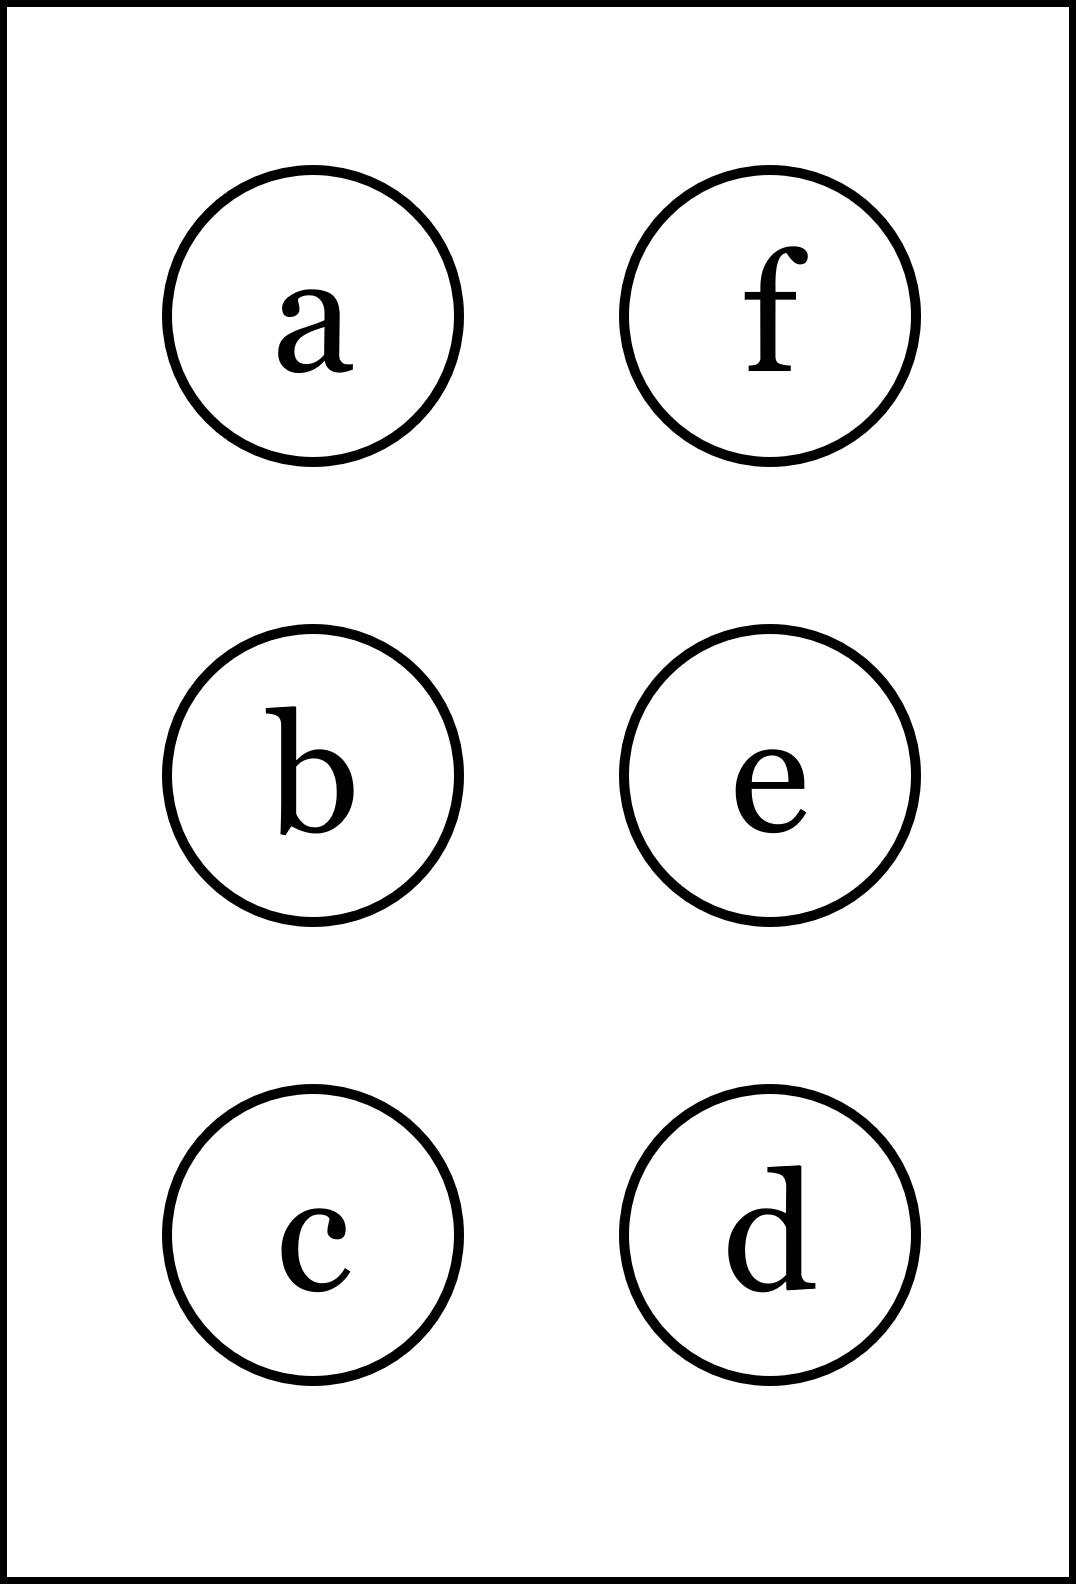
\includegraphics[height=40mm]{../images/braille.png}
{\small Písmeno Braillovej abecedy}
\end{center}
\end{minipage}
\end{center}
\end{minipage}
&
\begin{minipage}[c][104.5mm][t]{0.5\linewidth}
\begin{center}
\vspace{7mm}
{\huge Viazané extrémy, skupina \textit{Epsilon $\epsilon$} -\romannumeral4}\\[5mm]
\textit{Jméno:}\phantom{xxxxxxxxxxxxxxxxxxxxxxxxxxxxxxxxxxxxxxxxxxxxxxxxxxxxxxxxxxxxxxxxx}\\[5mm]
\begin{minipage}{0.95\linewidth}
\begin{center}
Cílem je najít \textbf{vázané extrémy} funkce $f(x,y)$ zadané v \textbf{(a)} spolu s vazbou (podmínkou). Postupuj podle krokú v \textbf{(b)} až \textbf{(f)}. Pokud se medzivýsledky shodujú s těmi za otazníky,\\tak napravo obarvi příslušející kroužek načerno. \textbf{Spolu odevzdejte výsledné slovo}.
\end{center}
\end{minipage}
\\[1mm]
\begin{minipage}{0.79\linewidth}
\begin{center}
\begin{varwidth}{\linewidth}
\begin{enumerate}
\normalsize
\item $f(x,y)=10x+24y+4 \enspace , \enspace \mathrm{vazba:} \enspace x^2+y^2=676$\quad \dotfill\; ???\;\dotfill \quad nebarvi
\item Sestav $L(\lambda,x,y)$ a spočti $\pdv{L}{x}=$\quad \dotfill\; ???\;\dotfill \quad $10+2\lambda x$
\item Takisto spočti $\pdv{L}{y}=$\quad \dotfill\; ???\;\dotfill \quad $24+2\lambda y$
\item Z podmínek $\pdv{L}{x}=0 , \pdv{L}{y}=0$ vyjádři $x,y$ v závislosti na $\lambda$.\\ \phantom{xxxxxx}Následne $x,y$ dosaď do vazbové rovnice\\ \phantom{xxxxxx}a vypočti dva výsledky pro $\lambda$.\quad \dotfill\; ???\;\dotfill \quad $\lambda_1+\lambda_2=-2$
\item Pomocou $\lambda$ urč dvě dvojice pro $x,y$.\quad \dotfill\; ???\;\dotfill \quad $x_1 x_2 y_1 y_2=57600$
\item Najdi funkční hodnoty pro oba vázané stacionární body\\ \phantom{xxxxxx}a vyber tu najvětší. $f_{\text{max}}(x,y)=$\quad \dotfill\; ???\;\dotfill \quad $680$
\end{enumerate}
\end{varwidth}
\end{center}
\end{minipage}
\begin{minipage}{0.20\linewidth}
\begin{center}
{\Huge\bfseries 4.} \\[2mm]
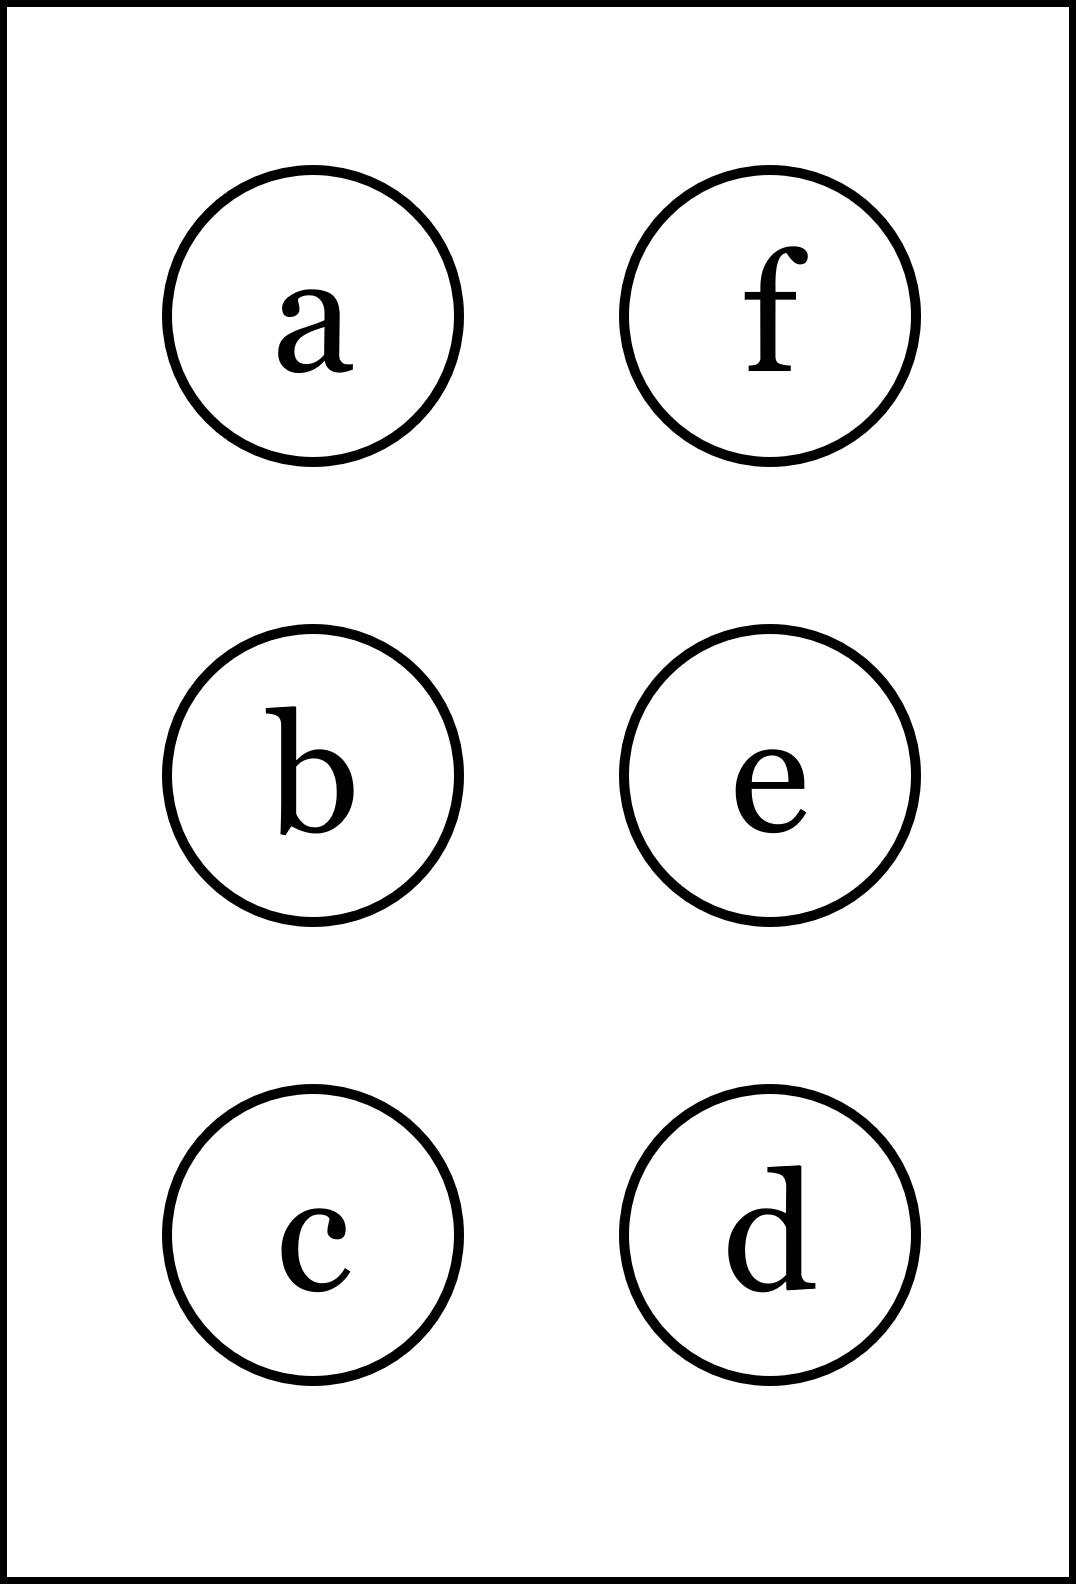
\includegraphics[height=40mm]{../images/braille.png}
{\small Písmeno Braillovej abecedy}
\end{center}
\end{minipage}
\end{center}
\end{minipage}
%
\end{tabular}
\newpage
\thispagestyle{empty}
\begin{tabular}{c:c}
\begin{minipage}[c][104.5mm][t]{0.5\linewidth}
\begin{center}
\vspace{7mm}
{\huge Viazané extrémy, skupina \textit{Zeta $\zeta$} -\romannumeral1}\\[5mm]
\textit{Jméno:}\phantom{xxxxxxxxxxxxxxxxxxxxxxxxxxxxxxxxxxxxxxxxxxxxxxxxxxxxxxxxxxxxxxxxx}\\[5mm]
\begin{minipage}{0.95\linewidth}
\begin{center}
Cílem je najít \textbf{vázané extrémy} funkce $f(x,y)$ zadané v \textbf{(a)} spolu s vazbou (podmínkou). Postupuj podle krokú v \textbf{(b)} až \textbf{(f)}. Pokud se medzivýsledky shodujú s těmi za otazníky,\\tak napravo obarvi příslušející kroužek načerno. \textbf{Spolu odevzdejte výsledné slovo}.
\end{center}
\end{minipage}
\\[1mm]
\begin{minipage}{0.79\linewidth}
\begin{center}
\begin{varwidth}{\linewidth}
\begin{enumerate}
\normalsize
\item $f(x,y)=3x-4y+5 \enspace , \enspace \mathrm{vazba:} \enspace x^2+y^2=25$\quad \dotfill\; ???\;\dotfill \quad nebarvi
\item Sestav $L(\lambda,x,y)$ a spočti $\pdv{L}{x}=$\quad \dotfill\; ???\;\dotfill \quad $3+\lambda x$
\item Takisto spočti $\pdv{L}{y}=$\quad \dotfill\; ???\;\dotfill \quad $-4+2\lambda y$
\item Z podmínek $\pdv{L}{x}=0 , \pdv{L}{y}=0$ vyjádři $x,y$ v závislosti na $\lambda$.\\ \phantom{xxxxxx}Následne $x,y$ dosaď do vazbové rovnice\\ \phantom{xxxxxx}a vypočti dva výsledky pro $\lambda$.\quad \dotfill\; ???\;\dotfill \quad $\lambda_1+\lambda_2=0$
\item Pomocou $\lambda$ urč dvě dvojice pro $x,y$.\quad \dotfill\; ???\;\dotfill \quad $x_1 x_2 y_1 y_2=-36$
\item Najdi funkční hodnoty pro oba vázané stacionární body\\ \phantom{xxxxxx}a vyber tu najvětší. $f_{\text{max}}(x,y)=$\quad \dotfill\; ???\;\dotfill \quad $30$
\end{enumerate}
\end{varwidth}
\end{center}
\end{minipage}
\begin{minipage}{0.20\linewidth}
\begin{center}
{\Huge\bfseries 1.} \\[2mm]
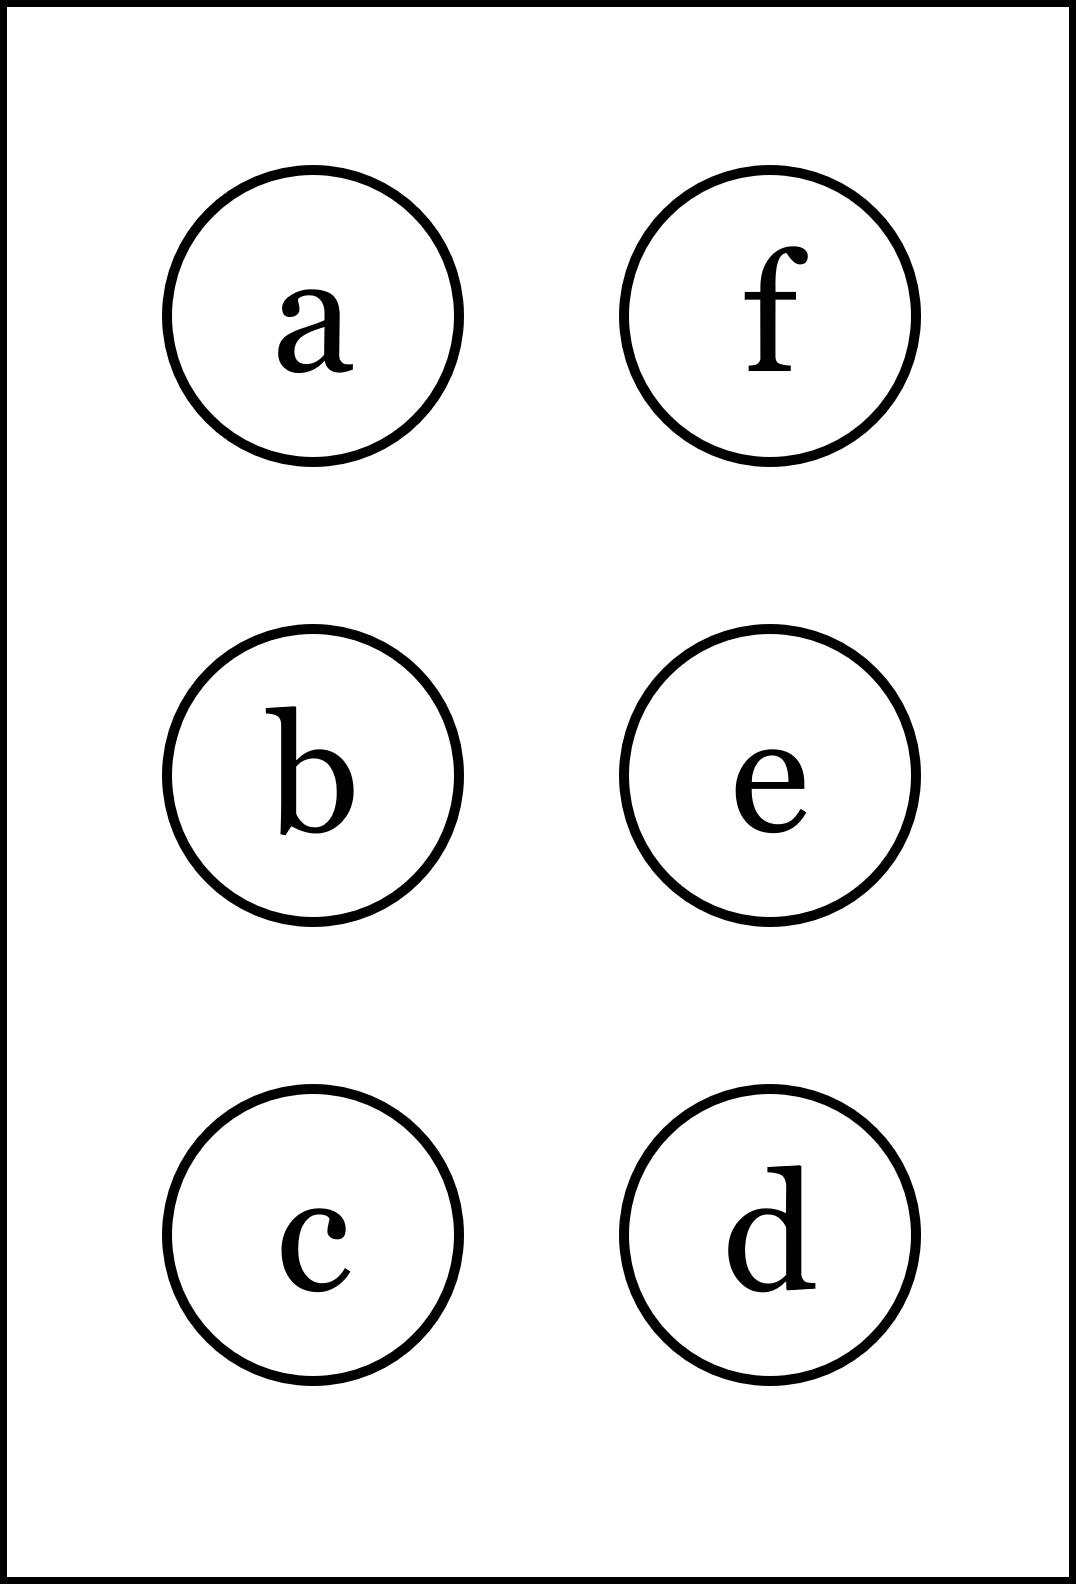
\includegraphics[height=40mm]{../images/braille.png}
{\small Písmeno Braillovej abecedy}
\end{center}
\end{minipage}
\end{center}
\end{minipage}
&
\begin{minipage}[c][104.5mm][t]{0.5\linewidth}
\begin{center}
\vspace{7mm}
{\huge Viazané extrémy, skupina \textit{Zeta $\zeta$} -\romannumeral2}\\[5mm]
\textit{Jméno:}\phantom{xxxxxxxxxxxxxxxxxxxxxxxxxxxxxxxxxxxxxxxxxxxxxxxxxxxxxxxxxxxxxxxxx}\\[5mm]
\begin{minipage}{0.95\linewidth}
\begin{center}
Cílem je najít \textbf{vázané extrémy} funkce $f(x,y)$ zadané v \textbf{(a)} spolu s vazbou (podmínkou). Postupuj podle krokú v \textbf{(b)} až \textbf{(f)}. Pokud se medzivýsledky shodujú s těmi za otazníky,\\tak napravo obarvi příslušející kroužek načerno. \textbf{Spolu odevzdejte výsledné slovo}.
\end{center}
\end{minipage}
\\[1mm]
\begin{minipage}{0.79\linewidth}
\begin{center}
\begin{varwidth}{\linewidth}
\begin{enumerate}
\normalsize
\item $f(x,y)=5x+12y-4 \enspace , \enspace \mathrm{vazba:} \enspace x^2+y^2=169$\quad \dotfill\; ???\;\dotfill \quad vybarvi
\item Sestav $L(\lambda,x,y)$ a spočti $\pdv{L}{x}=$\quad \dotfill\; ???\;\dotfill \quad $5+\lambda x$
\item Takisto spočti $\pdv{L}{y}=$\quad \dotfill\; ???\;\dotfill \quad $12+2\lambda y$
\item Z podmínek $\pdv{L}{x}=0 , \pdv{L}{y}=0$ vyjádři $x,y$ v závislosti na $\lambda$.\\ \phantom{xxxxxx}Následne $x,y$ dosaď do vazbové rovnice\\ \phantom{xxxxxx}a vypočti dva výsledky pro $\lambda$.\quad \dotfill\; ???\;\dotfill \quad $\lambda_1+\lambda_2=-1$
\item Pomocou $\lambda$ urč dvě dvojice pro $x,y$.\quad \dotfill\; ???\;\dotfill \quad $x_1 x_2 y_1 y_2=300$
\item Najdi funkční hodnoty pro oba vázané stacionární body\\ \phantom{xxxxxx}a vyber tu najvětší. $f_{\text{max}}(x,y)=$\quad \dotfill\; ???\;\dotfill \quad $164$
\end{enumerate}
\end{varwidth}
\end{center}
\end{minipage}
\begin{minipage}{0.20\linewidth}
\begin{center}
{\Huge\bfseries 2.} \\[2mm]
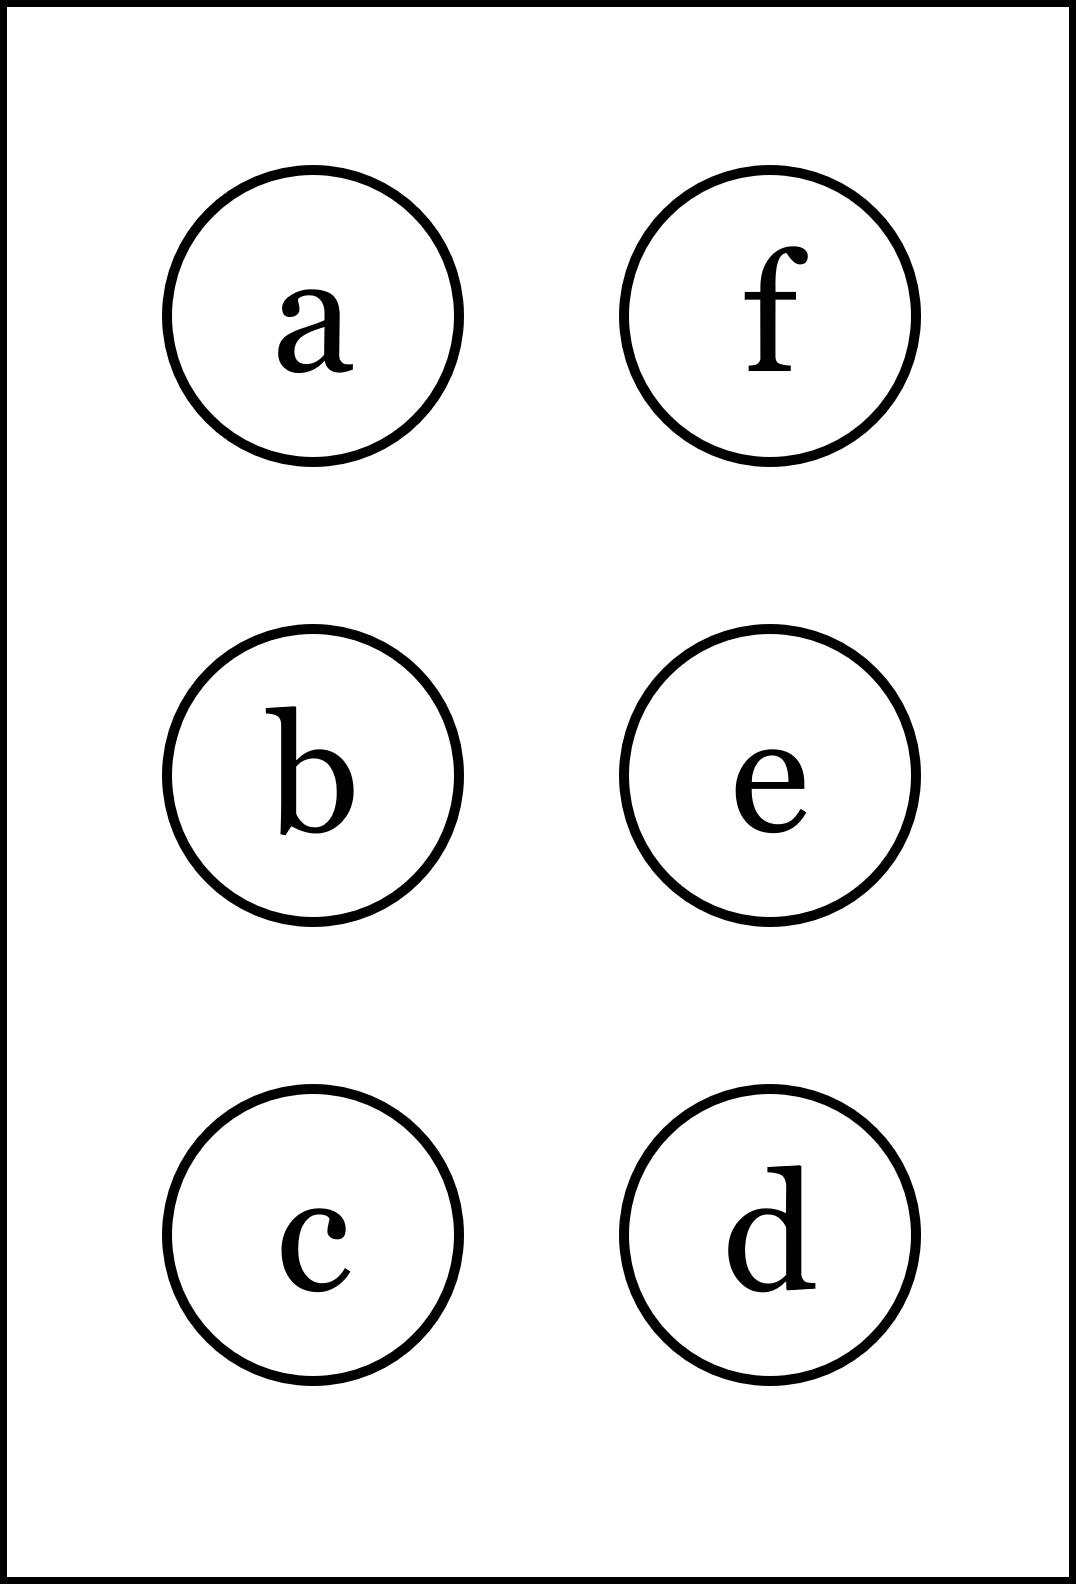
\includegraphics[height=40mm]{../images/braille.png}
{\small Písmeno Braillovej abecedy}
\end{center}
\end{minipage}
\end{center}
\end{minipage}
\\ \hdashline
\begin{minipage}[c][104.5mm][t]{0.5\linewidth}
\begin{center}
\vspace{7mm}
{\huge Viazané extrémy, skupina \textit{Zeta $\zeta$} -\romannumeral3}\\[5mm]
\textit{Jméno:}\phantom{xxxxxxxxxxxxxxxxxxxxxxxxxxxxxxxxxxxxxxxxxxxxxxxxxxxxxxxxxxxxxxxxx}\\[5mm]
\begin{minipage}{0.95\linewidth}
\begin{center}
Cílem je najít \textbf{vázané extrémy} funkce $f(x,y)$ zadané v \textbf{(a)} spolu s vazbou (podmínkou). Postupuj podle krokú v \textbf{(b)} až \textbf{(f)}. Pokud se medzivýsledky shodujú s těmi za otazníky,\\tak napravo obarvi příslušející kroužek načerno. \textbf{Spolu odevzdejte výsledné slovo}.
\end{center}
\end{minipage}
\\[1mm]
\begin{minipage}{0.79\linewidth}
\begin{center}
\begin{varwidth}{\linewidth}
\begin{enumerate}
\normalsize
\item $f(x,y)=-6x+8y+3 \enspace , \enspace \mathrm{vazba:} \enspace x^2+y^2=100$\quad \dotfill\; ???\;\dotfill \quad vybarvi
\item Sestav $L(\lambda,x,y)$ a spočti $\pdv{L}{x}=$\quad \dotfill\; ???\;\dotfill \quad $-6+\lambda x$
\item Takisto spočti $\pdv{L}{y}=$\quad \dotfill\; ???\;\dotfill \quad $8+2\lambda y$
\item Z podmínek $\pdv{L}{x}=0 , \pdv{L}{y}=0$ vyjádři $x,y$ v závislosti na $\lambda$.\\ \phantom{xxxxxx}Následne $x,y$ dosaď do vazbové rovnice\\ \phantom{xxxxxx}a vypočti dva výsledky pro $\lambda$.\quad \dotfill\; ???\;\dotfill \quad $\lambda_1+\lambda_2=-2$
\item Pomocou $\lambda$ urč dvě dvojice pro $x,y$.\quad \dotfill\; ???\;\dotfill \quad $x_1 x_2 y_1 y_2=2304$
\item Najdi funkční hodnoty pro oba vázané stacionární body\\ \phantom{xxxxxx}a vyber tu najvětší. $f_{\text{max}}(x,y)=$\quad \dotfill\; ???\;\dotfill \quad $102$
\end{enumerate}
\end{varwidth}
\end{center}
\end{minipage}
\begin{minipage}{0.20\linewidth}
\begin{center}
{\Huge\bfseries 3.} \\[2mm]
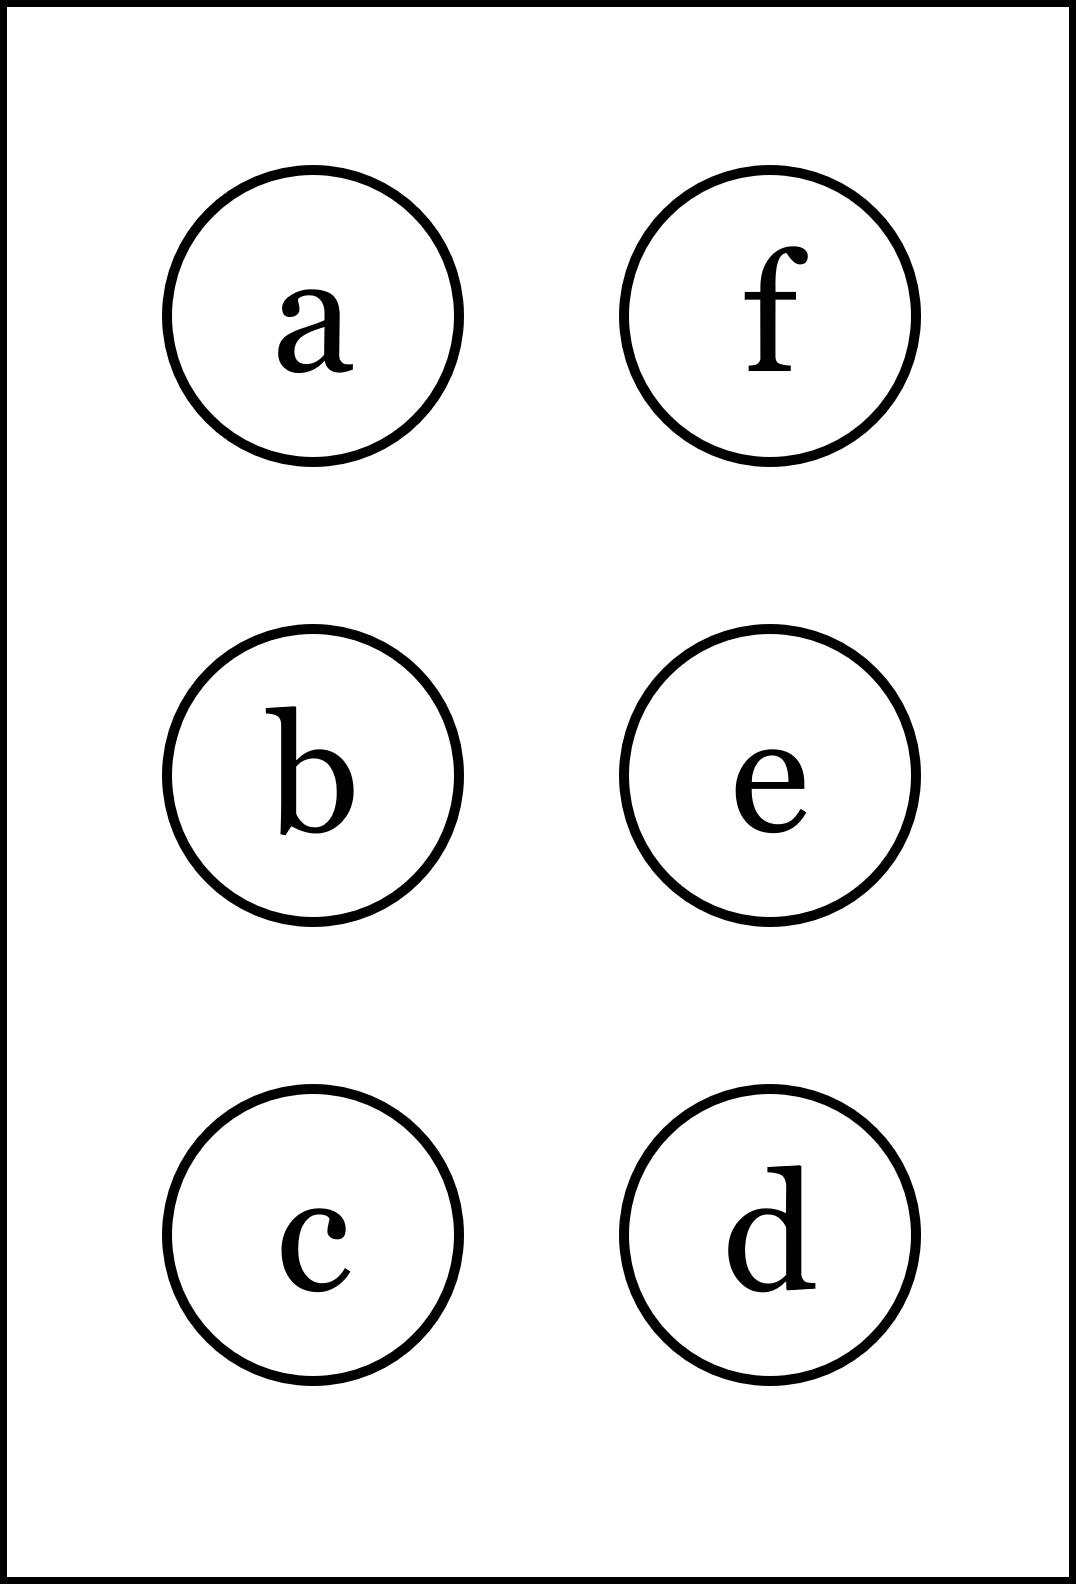
\includegraphics[height=40mm]{../images/braille.png}
{\small Písmeno Braillovej abecedy}
\end{center}
\end{minipage}
\end{center}
\end{minipage}
&
\begin{minipage}[c][104.5mm][t]{0.5\linewidth}
\begin{center}
\vspace{7mm}
{\huge Viazané extrémy, skupina \textit{Zeta $\zeta$} -\romannumeral4}\\[5mm]
\textit{Jméno:}\phantom{xxxxxxxxxxxxxxxxxxxxxxxxxxxxxxxxxxxxxxxxxxxxxxxxxxxxxxxxxxxxxxxxx}\\[5mm]
\begin{minipage}{0.95\linewidth}
\begin{center}
Cílem je najít \textbf{vázané extrémy} funkce $f(x,y)$ zadané v \textbf{(a)} spolu s vazbou (podmínkou). Postupuj podle krokú v \textbf{(b)} až \textbf{(f)}. Pokud se medzivýsledky shodujú s těmi za otazníky,\\tak napravo obarvi příslušející kroužek načerno. \textbf{Spolu odevzdejte výsledné slovo}.
\end{center}
\end{minipage}
\\[1mm]
\begin{minipage}{0.79\linewidth}
\begin{center}
\begin{varwidth}{\linewidth}
\begin{enumerate}
\normalsize
\item $f(x,y)=-10x+24y+1 \enspace , \enspace \mathrm{vazba:} \enspace x^2+y^2=676$\quad \dotfill\; ???\;\dotfill \quad vybarvi
\item Sestav $L(\lambda,x,y)$ a spočti $\pdv{L}{x}=$\quad \dotfill\; ???\;\dotfill \quad $-10+2\lambda x$
\item Takisto spočti $\pdv{L}{y}=$\quad \dotfill\; ???\;\dotfill \quad $24+2\lambda y$
\item Z podmínek $\pdv{L}{x}=0 , \pdv{L}{y}=0$ vyjádři $x,y$ v závislosti na $\lambda$.\\ \phantom{xxxxxx}Následne $x,y$ dosaď do vazbové rovnice\\ \phantom{xxxxxx}a vypočti dva výsledky pro $\lambda$.\quad \dotfill\; ???\;\dotfill \quad $\lambda_1+\lambda_2=-1$
\item Pomocou $\lambda$ urč dvě dvojice pro $x,y$.\quad \dotfill\; ???\;\dotfill \quad $x_1 x_2 y_1 y_2=2400$
\item Najdi funkční hodnoty pro oba vázané stacionární body\\ \phantom{xxxxxx}a vyber tu najvětší. $f_{\text{max}}(x,y)=$\quad \dotfill\; ???\;\dotfill \quad $676$
\end{enumerate}
\end{varwidth}
\end{center}
\end{minipage}
\begin{minipage}{0.20\linewidth}
\begin{center}
{\Huge\bfseries 4.} \\[2mm]
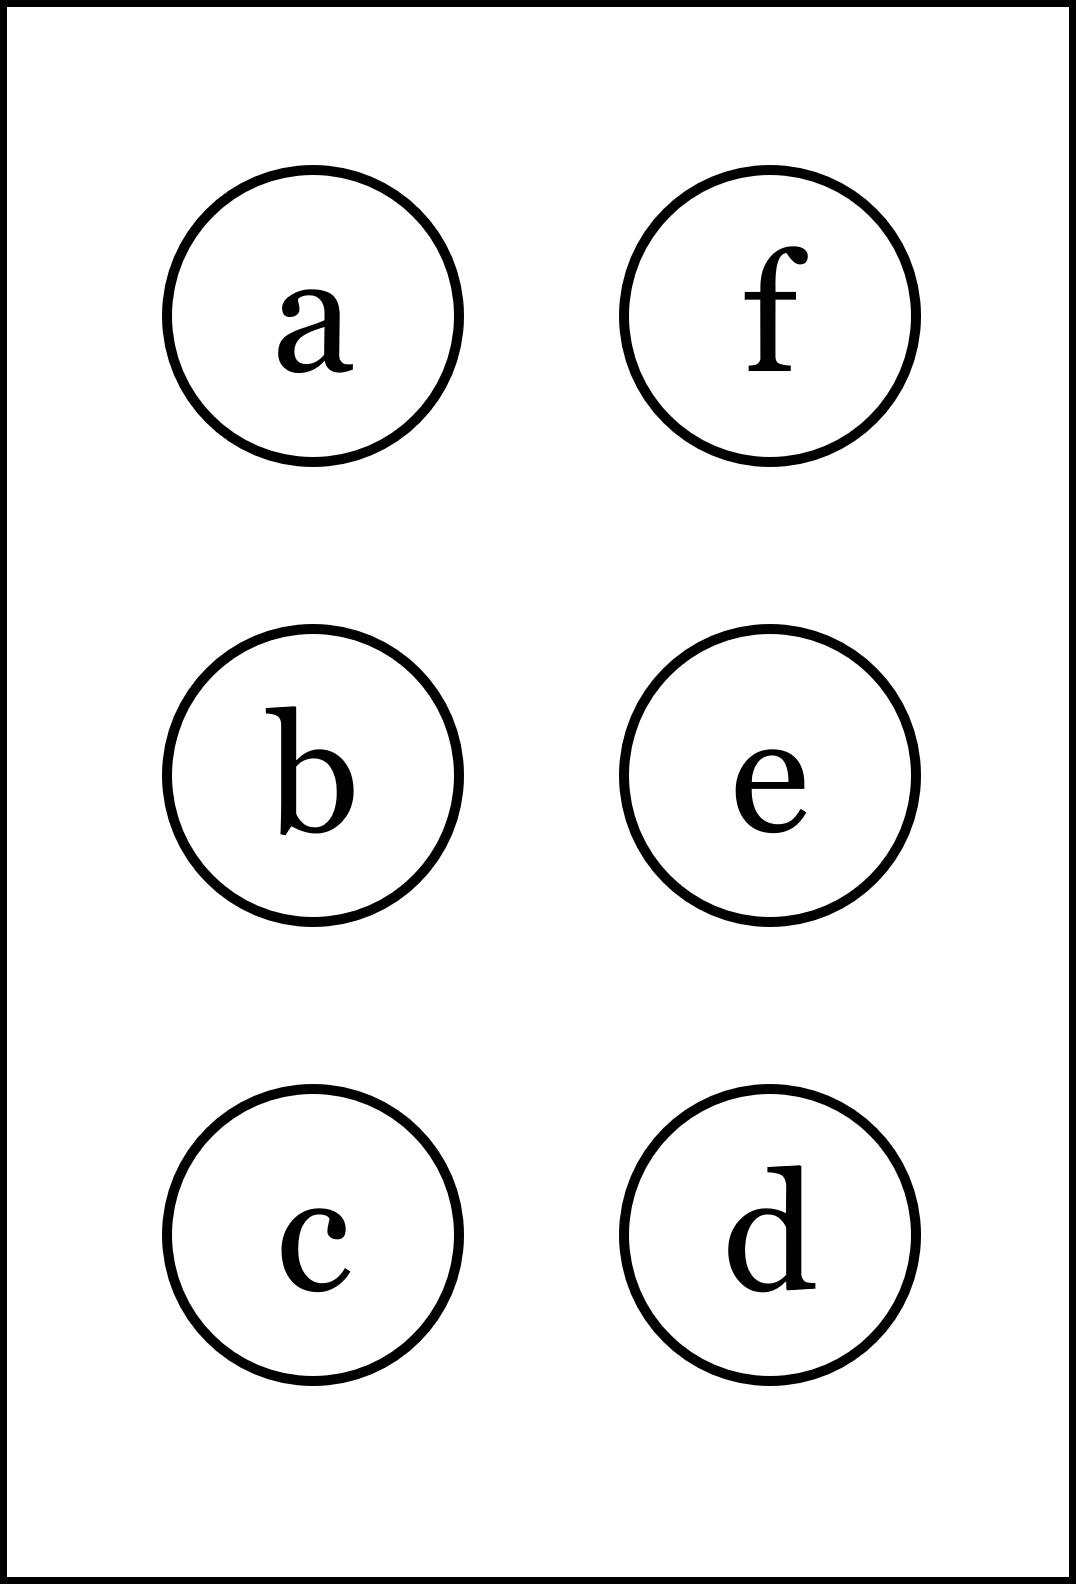
\includegraphics[height=40mm]{../images/braille.png}
{\small Písmeno Braillovej abecedy}
\end{center}
\end{minipage}
\end{center}
\end{minipage}
%
\end{tabular}
\newpage
\thispagestyle{empty}
\begin{tabular}{c:c}
\begin{minipage}[c][104.5mm][t]{0.5\linewidth}
\begin{center}
\vspace{7mm}
{\huge Viazané extrémy, skupina \textit{Eta $\eta$} -\romannumeral1}\\[5mm]
\textit{Jméno:}\phantom{xxxxxxxxxxxxxxxxxxxxxxxxxxxxxxxxxxxxxxxxxxxxxxxxxxxxxxxxxxxxxxxxx}\\[5mm]
\begin{minipage}{0.95\linewidth}
\begin{center}
Cílem je najít \textbf{vázané extrémy} funkce $f(x,y)$ zadané v \textbf{(a)} spolu s vazbou (podmínkou). Postupuj podle krokú v \textbf{(b)} až \textbf{(f)}. Pokud se medzivýsledky shodujú s těmi za otazníky,\\tak napravo obarvi příslušející kroužek načerno. \textbf{Spolu odevzdejte výsledné slovo}.
\end{center}
\end{minipage}
\\[1mm]
\begin{minipage}{0.79\linewidth}
\begin{center}
\begin{varwidth}{\linewidth}
\begin{enumerate}
\normalsize
\item $f(x,y)=3x+4y-3 \enspace , \enspace \mathrm{vazba:} \enspace x^2+y^2=25$\quad \dotfill\; ???\;\dotfill \quad vybarvi
\item Sestav $L(\lambda,x,y)$ a spočti $\pdv{L}{x}=$\quad \dotfill\; ???\;\dotfill \quad $3+2\lambda x$
\item Takisto spočti $\pdv{L}{y}=$\quad \dotfill\; ???\;\dotfill \quad $4+2\lambda y$
\item Z podmínek $\pdv{L}{x}=0 , \pdv{L}{y}=0$ vyjádři $x,y$ v závislosti na $\lambda$.\\ \phantom{xxxxxx}Následne $x,y$ dosaď do vazbové rovnice\\ \phantom{xxxxxx}a vypočti dva výsledky pro $\lambda$.\quad \dotfill\; ???\;\dotfill \quad $\lambda_1+\lambda_2=0$
\item Pomocou $\lambda$ urč dvě dvojice pro $x,y$.\quad \dotfill\; ???\;\dotfill \quad $x_1 x_2 y_1 y_2=144$
\item Najdi funkční hodnoty pro oba vázané stacionární body\\ \phantom{xxxxxx}a vyber tu najvětší. $f_{\text{max}}(x,y)=$\quad \dotfill\; ???\;\dotfill \quad $21$
\end{enumerate}
\end{varwidth}
\end{center}
\end{minipage}
\begin{minipage}{0.20\linewidth}
\begin{center}
{\Huge\bfseries 1.} \\[2mm]
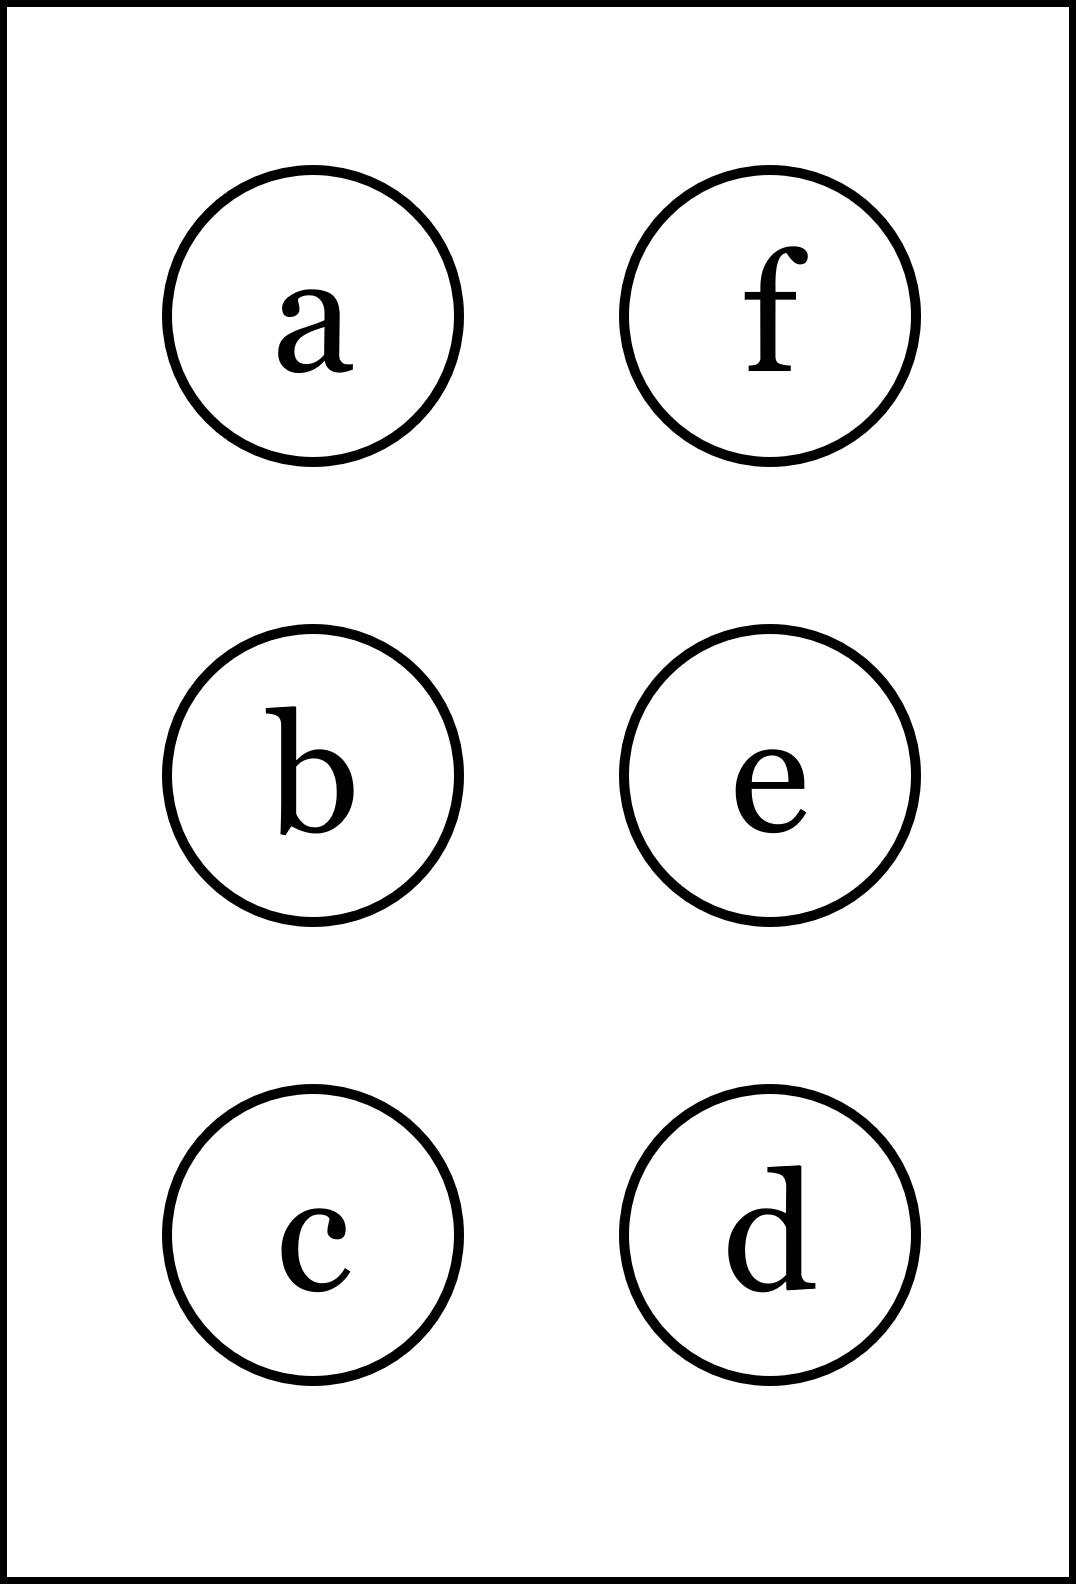
\includegraphics[height=40mm]{../images/braille.png}
{\small Písmeno Braillovej abecedy}
\end{center}
\end{minipage}
\end{center}
\end{minipage}
&
\begin{minipage}[c][104.5mm][t]{0.5\linewidth}
\begin{center}
\vspace{7mm}
{\huge Viazané extrémy, skupina \textit{Eta $\eta$} -\romannumeral2}\\[5mm]
\textit{Jméno:}\phantom{xxxxxxxxxxxxxxxxxxxxxxxxxxxxxxxxxxxxxxxxxxxxxxxxxxxxxxxxxxxxxxxxx}\\[5mm]
\begin{minipage}{0.95\linewidth}
\begin{center}
Cílem je najít \textbf{vázané extrémy} funkce $f(x,y)$ zadané v \textbf{(a)} spolu s vazbou (podmínkou). Postupuj podle krokú v \textbf{(b)} až \textbf{(f)}. Pokud se medzivýsledky shodujú s těmi za otazníky,\\tak napravo obarvi příslušející kroužek načerno. \textbf{Spolu odevzdejte výsledné slovo}.
\end{center}
\end{minipage}
\\[1mm]
\begin{minipage}{0.79\linewidth}
\begin{center}
\begin{varwidth}{\linewidth}
\begin{enumerate}
\normalsize
\item $f(x,y)=5x-12y-2 \enspace , \enspace \mathrm{vazba:} \enspace x^2+y^2=169$\quad \dotfill\; ???\;\dotfill \quad vybarvi
\item Sestav $L(\lambda,x,y)$ a spočti $\pdv{L}{x}=$\quad \dotfill\; ???\;\dotfill \quad $5+\lambda x$
\item Takisto spočti $\pdv{L}{y}=$\quad \dotfill\; ???\;\dotfill \quad $-12+2\lambda y$
\item Z podmínek $\pdv{L}{x}=0 , \pdv{L}{y}=0$ vyjádři $x,y$ v závislosti na $\lambda$.\\ \phantom{xxxxxx}Následne $x,y$ dosaď do vazbové rovnice\\ \phantom{xxxxxx}a vypočti dva výsledky pro $\lambda$.\quad \dotfill\; ???\;\dotfill \quad $\lambda_1+\lambda_2=2$
\item Pomocou $\lambda$ urč dvě dvojice pro $x,y$.\quad \dotfill\; ???\;\dotfill \quad $x_1 x_2 y_1 y_2=3600$
\item Najdi funkční hodnoty pro oba vázané stacionární body\\ \phantom{xxxxxx}a vyber tu najvětší. $f_{\text{max}}(x,y)=$\quad \dotfill\; ???\;\dotfill \quad $166$
\end{enumerate}
\end{varwidth}
\end{center}
\end{minipage}
\begin{minipage}{0.20\linewidth}
\begin{center}
{\Huge\bfseries 2.} \\[2mm]
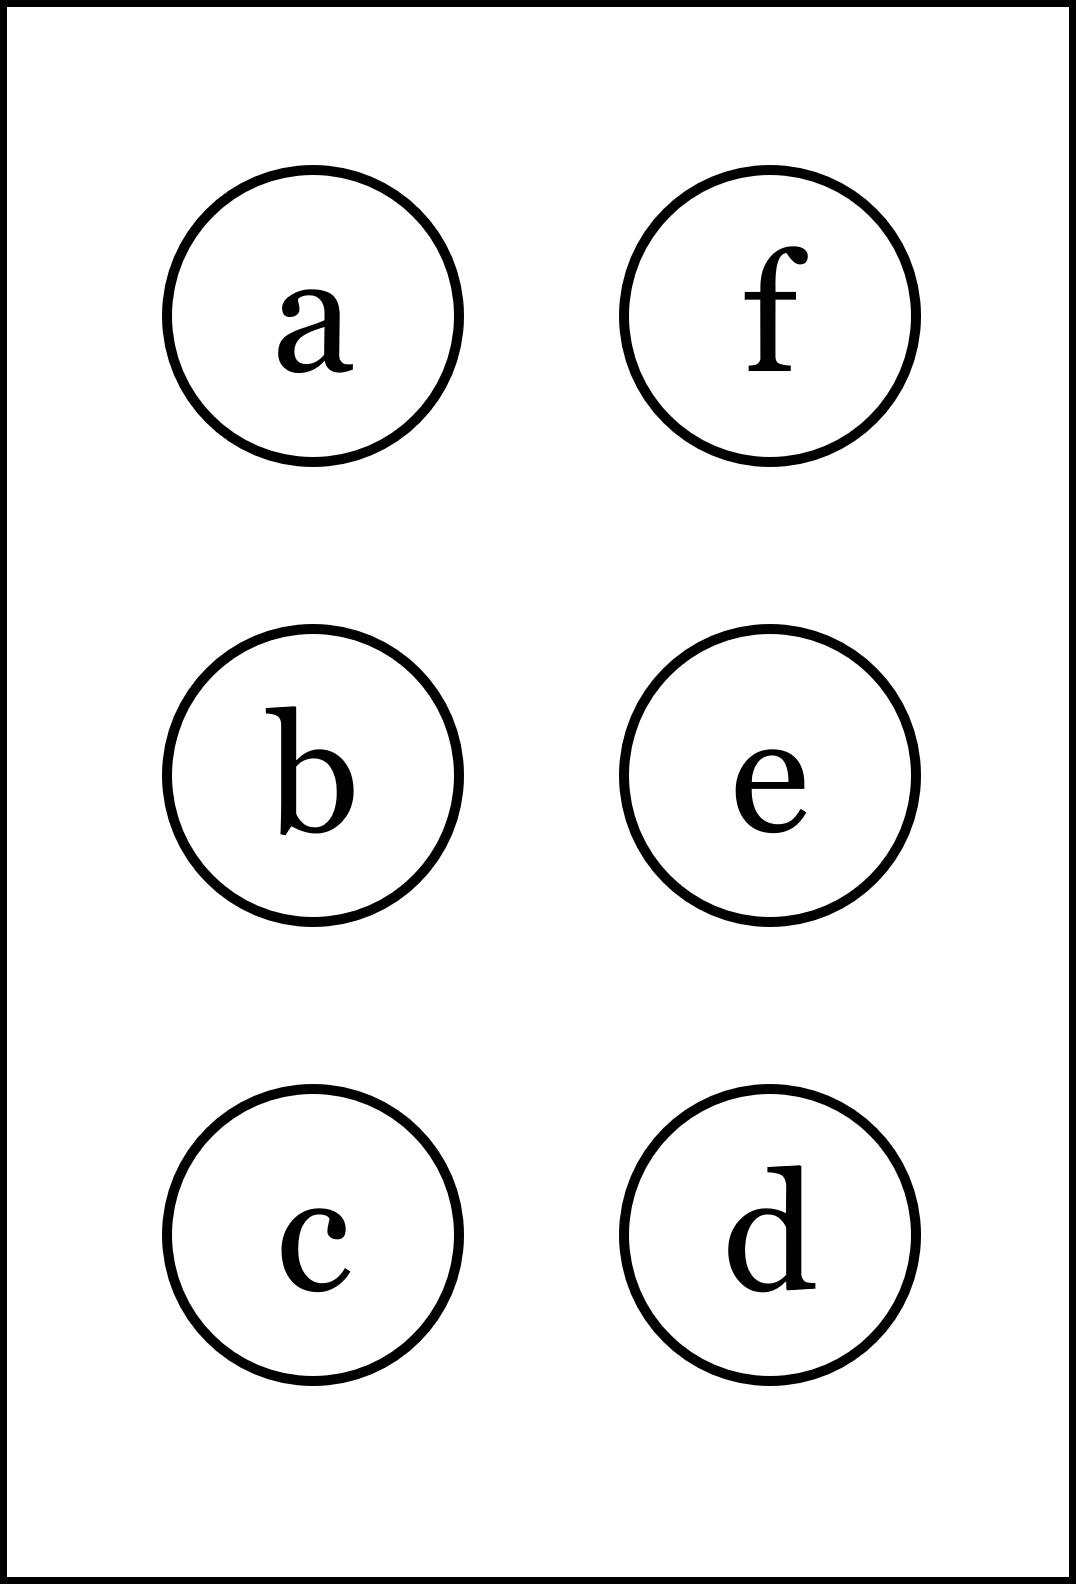
\includegraphics[height=40mm]{../images/braille.png}
{\small Písmeno Braillovej abecedy}
\end{center}
\end{minipage}
\end{center}
\end{minipage}
\\ \hdashline
\begin{minipage}[c][104.5mm][t]{0.5\linewidth}
\begin{center}
\vspace{7mm}
{\huge Viazané extrémy, skupina \textit{Eta $\eta$} -\romannumeral3}\\[5mm]
\textit{Jméno:}\phantom{xxxxxxxxxxxxxxxxxxxxxxxxxxxxxxxxxxxxxxxxxxxxxxxxxxxxxxxxxxxxxxxxx}\\[5mm]
\begin{minipage}{0.95\linewidth}
\begin{center}
Cílem je najít \textbf{vázané extrémy} funkce $f(x,y)$ zadané v \textbf{(a)} spolu s vazbou (podmínkou). Postupuj podle krokú v \textbf{(b)} až \textbf{(f)}. Pokud se medzivýsledky shodujú s těmi za otazníky,\\tak napravo obarvi příslušející kroužek načerno. \textbf{Spolu odevzdejte výsledné slovo}.
\end{center}
\end{minipage}
\\[1mm]
\begin{minipage}{0.79\linewidth}
\begin{center}
\begin{varwidth}{\linewidth}
\begin{enumerate}
\normalsize
\item $f(x,y)=-6x+8y+1 \enspace , \enspace \mathrm{vazba:} \enspace x^2+y^2=100$\quad \dotfill\; ???\;\dotfill \quad vybarvi
\item Sestav $L(\lambda,x,y)$ a spočti $\pdv{L}{x}=$\quad \dotfill\; ???\;\dotfill \quad $-6+2\lambda x$
\item Takisto spočti $\pdv{L}{y}=$\quad \dotfill\; ???\;\dotfill \quad $8+2\lambda y$
\item Z podmínek $\pdv{L}{x}=0 , \pdv{L}{y}=0$ vyjádři $x,y$ v závislosti na $\lambda$.\\ \phantom{xxxxxx}Následne $x,y$ dosaď do vazbové rovnice\\ \phantom{xxxxxx}a vypočti dva výsledky pro $\lambda$.\quad \dotfill\; ???\;\dotfill \quad $\lambda_1+\lambda_2=-2$
\item Pomocou $\lambda$ urč dvě dvojice pro $x,y$.\quad \dotfill\; ???\;\dotfill \quad $x_1 x_2 y_1 y_2=2304$
\item Najdi funkční hodnoty pro oba vázané stacionární body\\ \phantom{xxxxxx}a vyber tu najvětší. $f_{\text{max}}(x,y)=$\quad \dotfill\; ???\;\dotfill \quad $100$
\end{enumerate}
\end{varwidth}
\end{center}
\end{minipage}
\begin{minipage}{0.20\linewidth}
\begin{center}
{\Huge\bfseries 3.} \\[2mm]
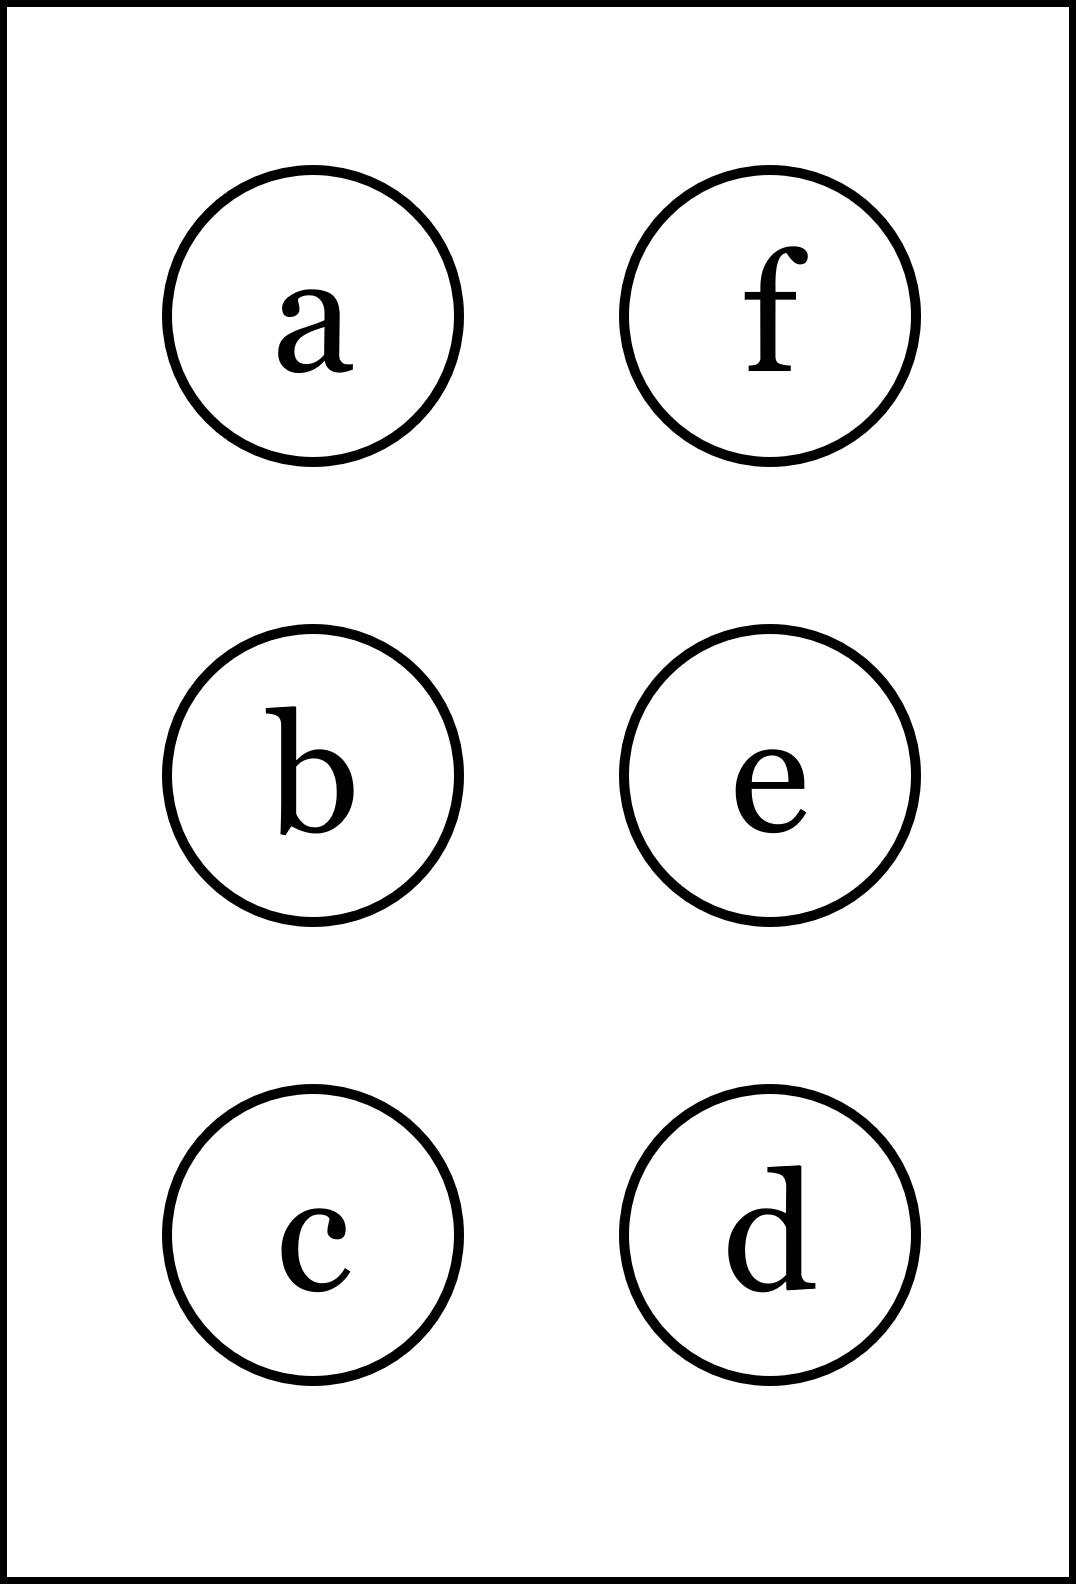
\includegraphics[height=40mm]{../images/braille.png}
{\small Písmeno Braillovej abecedy}
\end{center}
\end{minipage}
\end{center}
\end{minipage}
&
\begin{minipage}[c][104.5mm][t]{0.5\linewidth}
\begin{center}
\vspace{7mm}
{\huge Viazané extrémy, skupina \textit{Eta $\eta$} -\romannumeral4}\\[5mm]
\textit{Jméno:}\phantom{xxxxxxxxxxxxxxxxxxxxxxxxxxxxxxxxxxxxxxxxxxxxxxxxxxxxxxxxxxxxxxxxx}\\[5mm]
\begin{minipage}{0.95\linewidth}
\begin{center}
Cílem je najít \textbf{vázané extrémy} funkce $f(x,y)$ zadané v \textbf{(a)} spolu s vazbou (podmínkou). Postupuj podle krokú v \textbf{(b)} až \textbf{(f)}. Pokud se medzivýsledky shodujú s těmi za otazníky,\\tak napravo obarvi příslušející kroužek načerno. \textbf{Spolu odevzdejte výsledné slovo}.
\end{center}
\end{minipage}
\\[1mm]
\begin{minipage}{0.79\linewidth}
\begin{center}
\begin{varwidth}{\linewidth}
\begin{enumerate}
\normalsize
\item $f(x,y)=-10x+24y-7 \enspace , \enspace \mathrm{vazba:} \enspace x^2+y^2=676$\quad \dotfill\; ???\;\dotfill \quad vybarvi
\item Sestav $L(\lambda,x,y)$ a spočti $\pdv{L}{x}=$\quad \dotfill\; ???\;\dotfill \quad $-10+\lambda x$
\item Takisto spočti $\pdv{L}{y}=$\quad \dotfill\; ???\;\dotfill \quad $-24+2\lambda y$
\item Z podmínek $\pdv{L}{x}=0 , \pdv{L}{y}=0$ vyjádři $x,y$ v závislosti na $\lambda$.\\ \phantom{xxxxxx}Následne $x,y$ dosaď do vazbové rovnice\\ \phantom{xxxxxx}a vypočti dva výsledky pro $\lambda$.\quad \dotfill\; ???\;\dotfill \quad $\lambda_1+\lambda_2=2$
\item Pomocou $\lambda$ urč dvě dvojice pro $x,y$.\quad \dotfill\; ???\;\dotfill \quad $x_1 x_2 y_1 y_2=57600$
\item Najdi funkční hodnoty pro oba vázané stacionární body\\ \phantom{xxxxxx}a vyber tu najvětší. $f_{\text{max}}(x,y)=$\quad \dotfill\; ???\;\dotfill \quad $669$
\end{enumerate}
\end{varwidth}
\end{center}
\end{minipage}
\begin{minipage}{0.20\linewidth}
\begin{center}
{\Huge\bfseries 4.} \\[2mm]
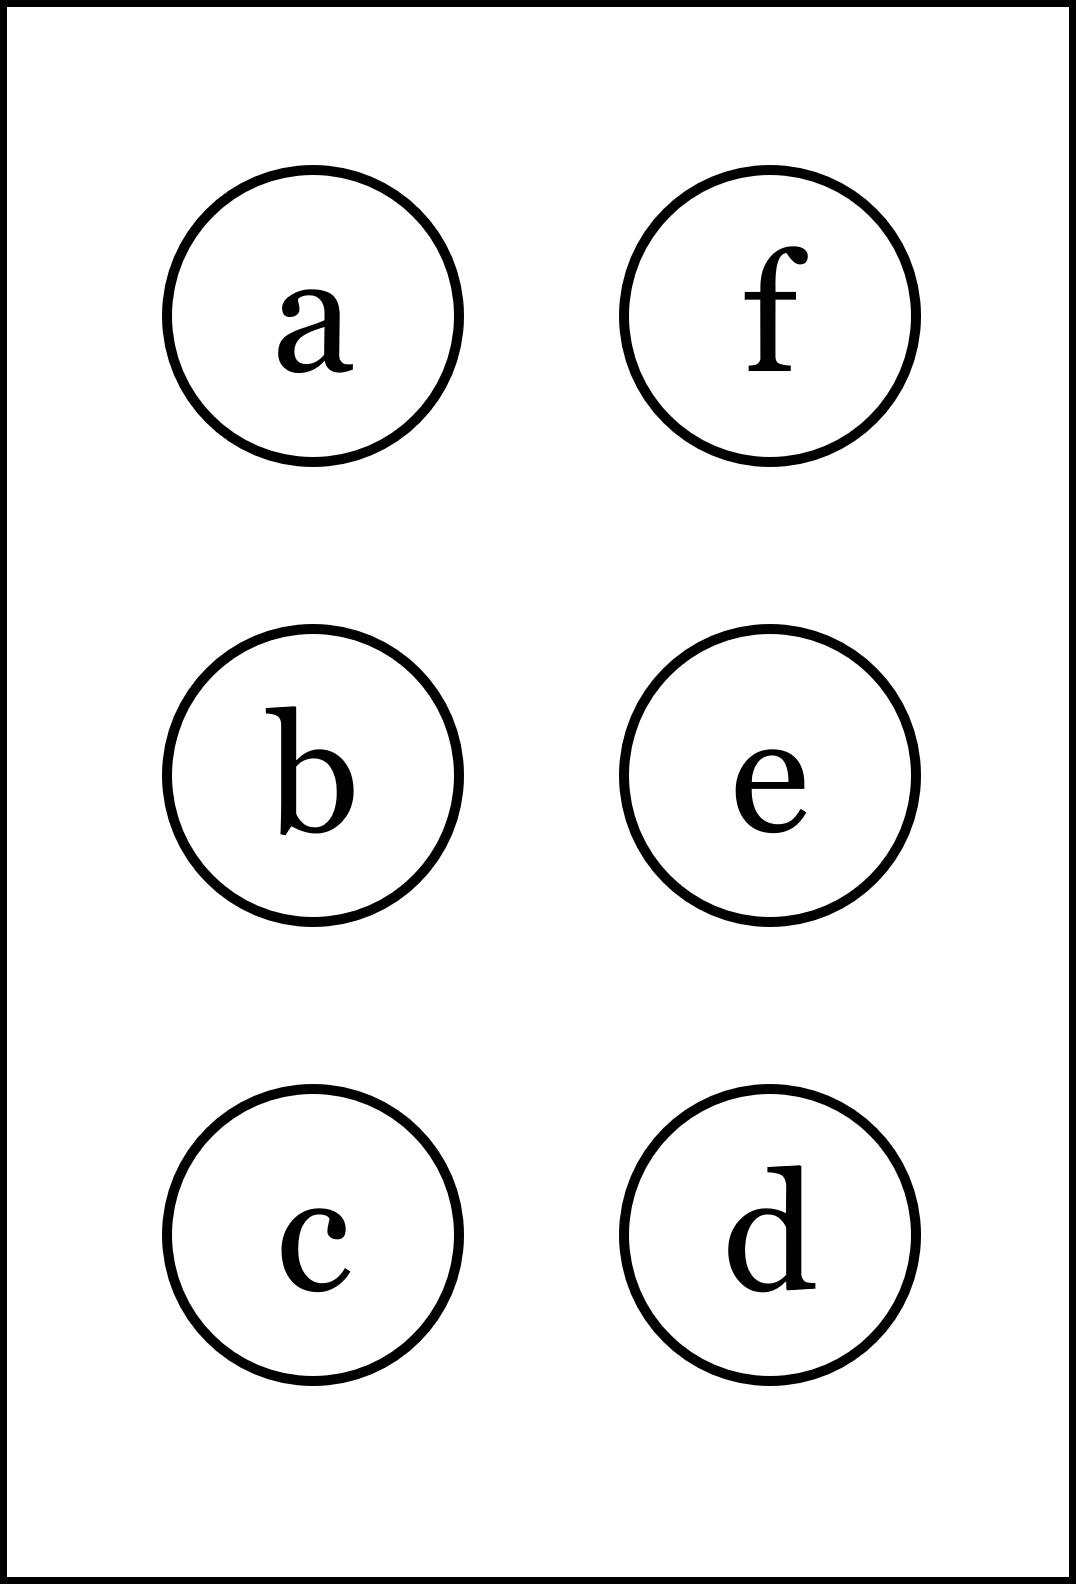
\includegraphics[height=40mm]{../images/braille.png}
{\small Písmeno Braillovej abecedy}
\end{center}
\end{minipage}
\end{center}
\end{minipage}
%
\end{tabular}
\newpage
\thispagestyle{empty}
\begin{tabular}{c:c}
\begin{minipage}[c][104.5mm][t]{0.5\linewidth}
\begin{center}
\vspace{7mm}
{\huge Viazané extrémy, skupina \textit{Theta $\theta$} -\romannumeral1}\\[5mm]
\textit{Jméno:}\phantom{xxxxxxxxxxxxxxxxxxxxxxxxxxxxxxxxxxxxxxxxxxxxxxxxxxxxxxxxxxxxxxxxx}\\[5mm]
\begin{minipage}{0.95\linewidth}
\begin{center}
Cílem je najít \textbf{vázané extrémy} funkce $f(x,y)$ zadané v \textbf{(a)} spolu s vazbou (podmínkou). Postupuj podle krokú v \textbf{(b)} až \textbf{(f)}. Pokud se medzivýsledky shodujú s těmi za otazníky,\\tak napravo obarvi příslušející kroužek načerno. \textbf{Spolu odevzdejte výsledné slovo}.
\end{center}
\end{minipage}
\\[1mm]
\begin{minipage}{0.79\linewidth}
\begin{center}
\begin{varwidth}{\linewidth}
\begin{enumerate}
\normalsize
\item $f(x,y)=-3x-4y+3 \enspace , \enspace \mathrm{vazba:} \enspace x^2+y^2=25$\quad \dotfill\; ???\;\dotfill \quad vybarvi
\item Sestav $L(\lambda,x,y)$ a spočti $\pdv{L}{x}=$\quad \dotfill\; ???\;\dotfill \quad $-3+2\lambda x$
\item Takisto spočti $\pdv{L}{y}=$\quad \dotfill\; ???\;\dotfill \quad $-4+2\lambda y$
\item Z podmínek $\pdv{L}{x}=0 , \pdv{L}{y}=0$ vyjádři $x,y$ v závislosti na $\lambda$.\\ \phantom{xxxxxx}Následne $x,y$ dosaď do vazbové rovnice\\ \phantom{xxxxxx}a vypočti dva výsledky pro $\lambda$.\quad \dotfill\; ???\;\dotfill \quad $\lambda_1+\lambda_2=-2$
\item Pomocou $\lambda$ urč dvě dvojice pro $x,y$.\quad \dotfill\; ???\;\dotfill \quad $x_1 x_2 y_1 y_2=144$
\item Najdi funkční hodnoty pro oba vázané stacionární body\\ \phantom{xxxxxx}a vyber tu najvětší. $f_{\text{max}}(x,y)=$\quad \dotfill\; ???\;\dotfill \quad $27$
\end{enumerate}
\end{varwidth}
\end{center}
\end{minipage}
\begin{minipage}{0.20\linewidth}
\begin{center}
{\Huge\bfseries 1.} \\[2mm]
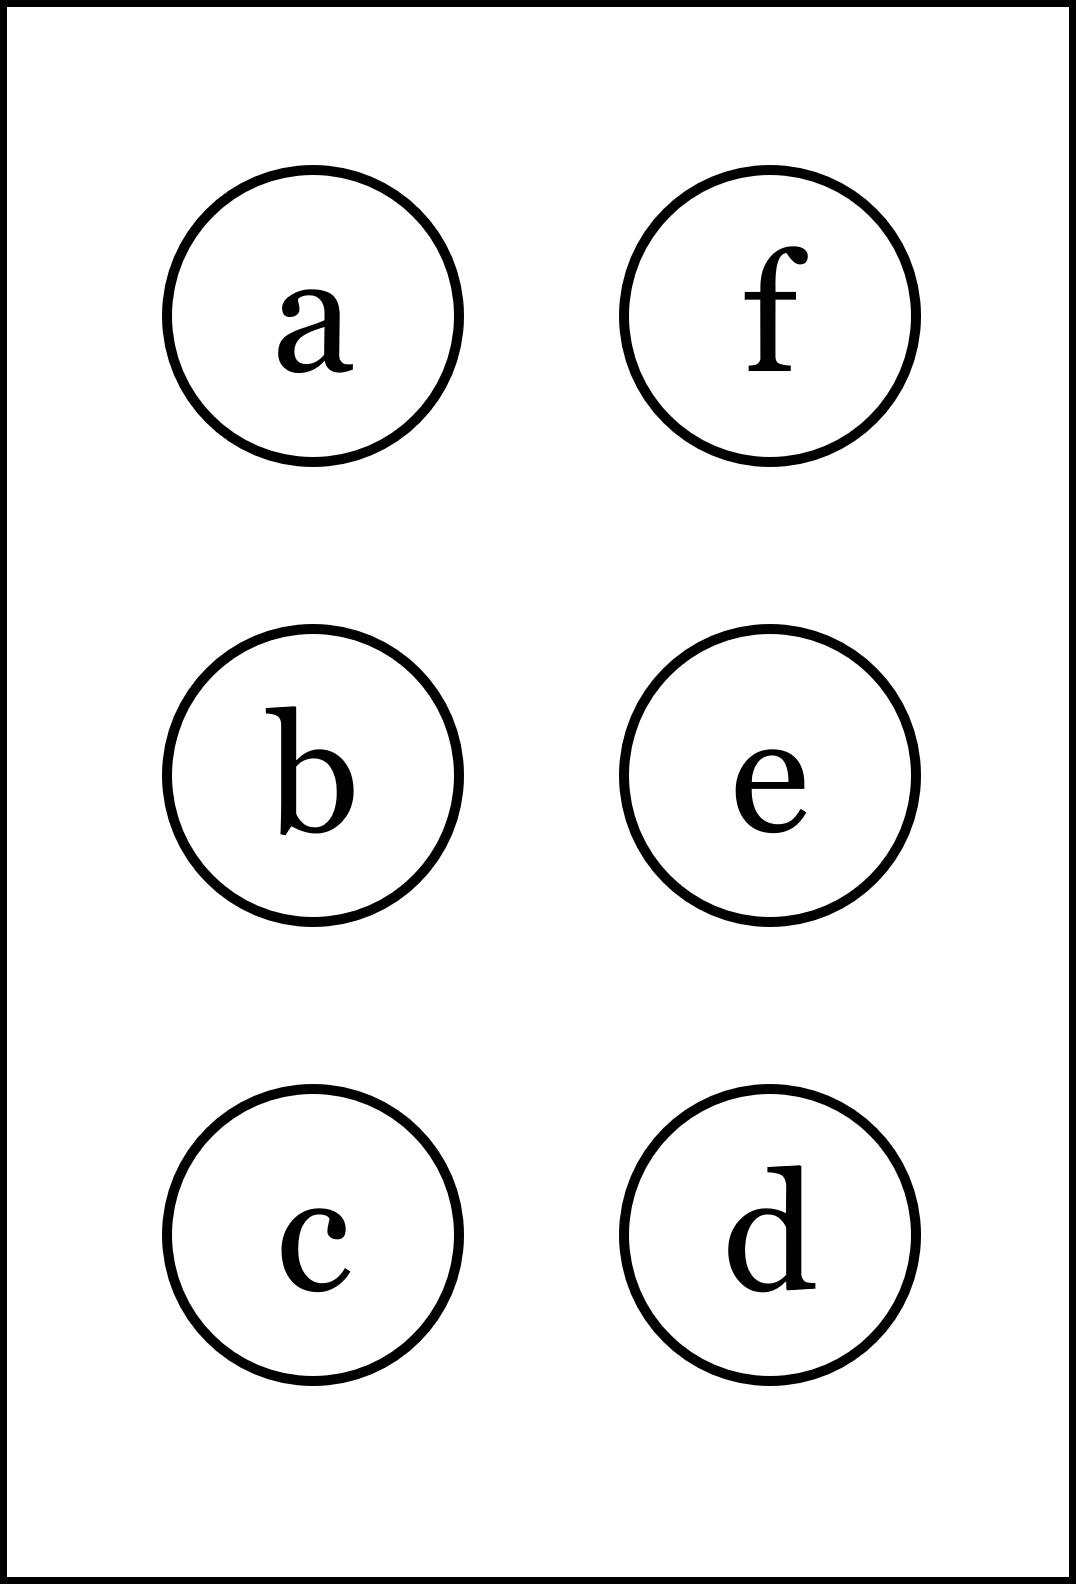
\includegraphics[height=40mm]{../images/braille.png}
{\small Písmeno Braillovej abecedy}
\end{center}
\end{minipage}
\end{center}
\end{minipage}
&
\begin{minipage}[c][104.5mm][t]{0.5\linewidth}
\begin{center}
\vspace{7mm}
{\huge Viazané extrémy, skupina \textit{Theta $\theta$} -\romannumeral2}\\[5mm]
\textit{Jméno:}\phantom{xxxxxxxxxxxxxxxxxxxxxxxxxxxxxxxxxxxxxxxxxxxxxxxxxxxxxxxxxxxxxxxxx}\\[5mm]
\begin{minipage}{0.95\linewidth}
\begin{center}
Cílem je najít \textbf{vázané extrémy} funkce $f(x,y)$ zadané v \textbf{(a)} spolu s vazbou (podmínkou). Postupuj podle krokú v \textbf{(b)} až \textbf{(f)}. Pokud se medzivýsledky shodujú s těmi za otazníky,\\tak napravo obarvi příslušející kroužek načerno. \textbf{Spolu odevzdejte výsledné slovo}.
\end{center}
\end{minipage}
\\[1mm]
\begin{minipage}{0.79\linewidth}
\begin{center}
\begin{varwidth}{\linewidth}
\begin{enumerate}
\normalsize
\item $f(x,y)=5x+12y+2 \enspace , \enspace \mathrm{vazba:} \enspace x^2+y^2=169$\quad \dotfill\; ???\;\dotfill \quad vybarvi
\item Sestav $L(\lambda,x,y)$ a spočti $\pdv{L}{x}=$\quad \dotfill\; ???\;\dotfill \quad $5+\lambda x$
\item Takisto spočti $\pdv{L}{y}=$\quad \dotfill\; ???\;\dotfill \quad $-12+2\lambda y$
\item Z podmínek $\pdv{L}{x}=0 , \pdv{L}{y}=0$ vyjádři $x,y$ v závislosti na $\lambda$.\\ \phantom{xxxxxx}Následne $x,y$ dosaď do vazbové rovnice\\ \phantom{xxxxxx}a vypočti dva výsledky pro $\lambda$.\quad \dotfill\; ???\;\dotfill \quad $\lambda_1+\lambda_2=2$
\item Pomocou $\lambda$ urč dvě dvojice pro $x,y$.\quad \dotfill\; ???\;\dotfill \quad $x_1 x_2 y_1 y_2=300$
\item Najdi funkční hodnoty pro oba vázané stacionární body\\ \phantom{xxxxxx}a vyber tu najvětší. $f_{\text{max}}(x,y)=$\quad \dotfill\; ???\;\dotfill \quad $170$
\end{enumerate}
\end{varwidth}
\end{center}
\end{minipage}
\begin{minipage}{0.20\linewidth}
\begin{center}
{\Huge\bfseries 2.} \\[2mm]
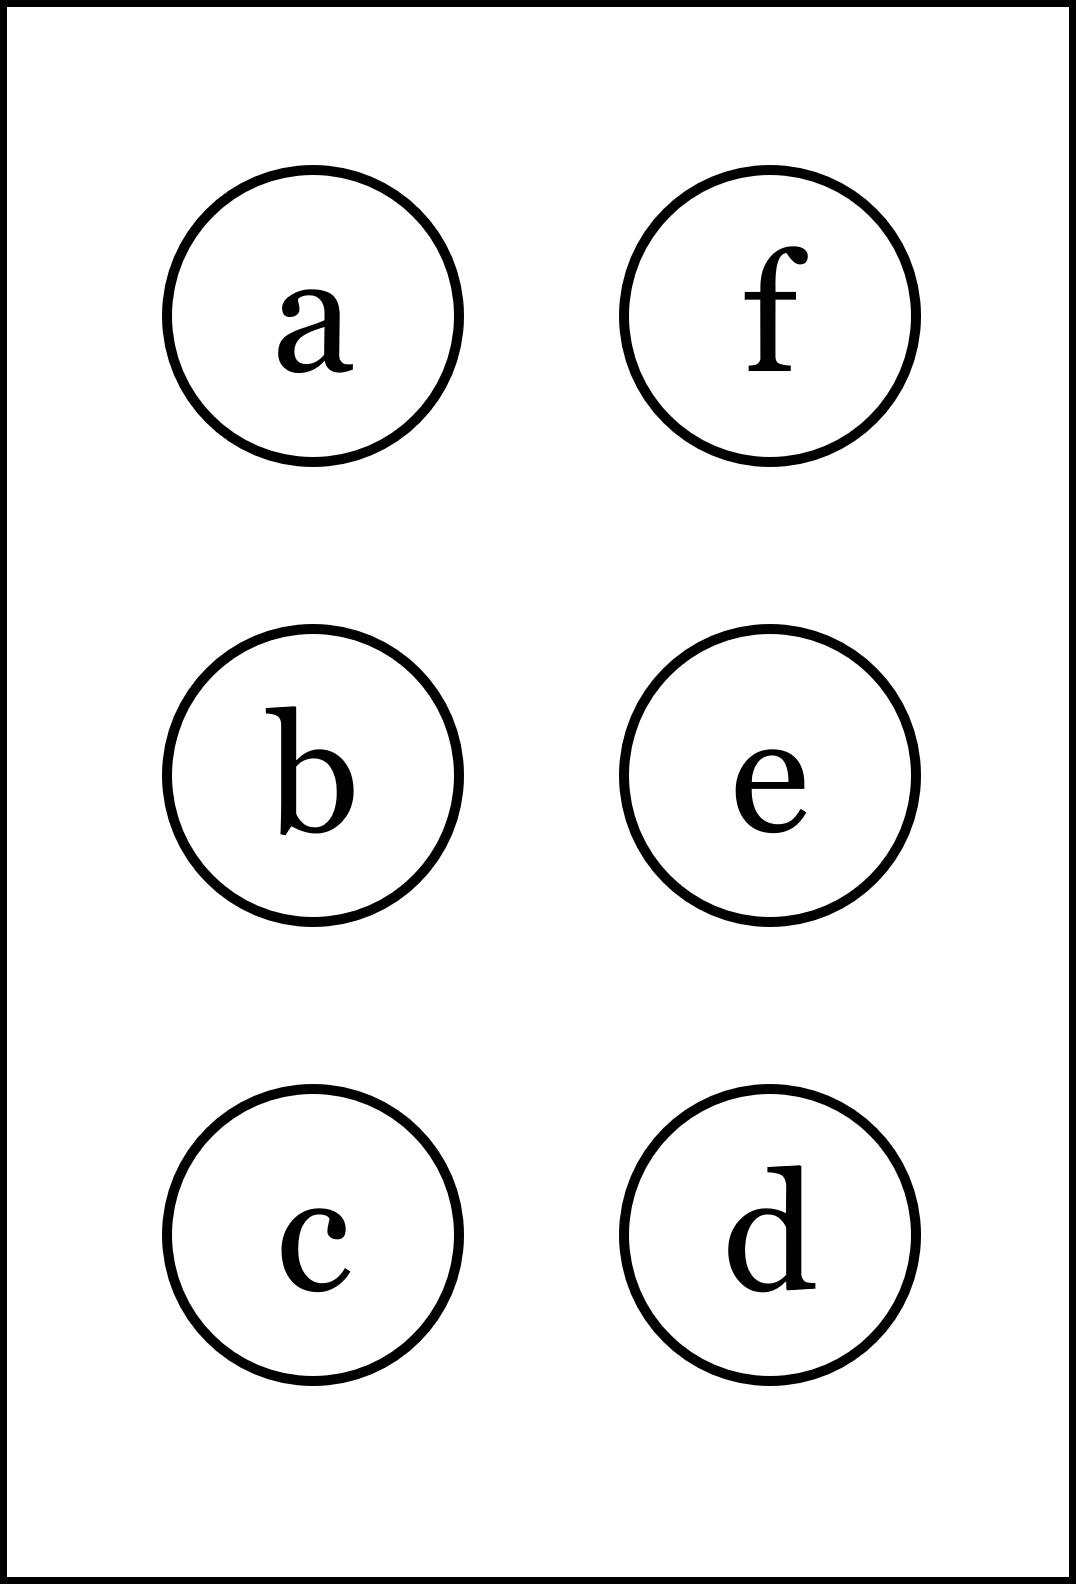
\includegraphics[height=40mm]{../images/braille.png}
{\small Písmeno Braillovej abecedy}
\end{center}
\end{minipage}
\end{center}
\end{minipage}
\\ \hdashline
\begin{minipage}[c][104.5mm][t]{0.5\linewidth}
\begin{center}
\vspace{7mm}
{\huge Viazané extrémy, skupina \textit{Theta $\theta$} -\romannumeral3}\\[5mm]
\textit{Jméno:}\phantom{xxxxxxxxxxxxxxxxxxxxxxxxxxxxxxxxxxxxxxxxxxxxxxxxxxxxxxxxxxxxxxxxx}\\[5mm]
\begin{minipage}{0.95\linewidth}
\begin{center}
Cílem je najít \textbf{vázané extrémy} funkce $f(x,y)$ zadané v \textbf{(a)} spolu s vazbou (podmínkou). Postupuj podle krokú v \textbf{(b)} až \textbf{(f)}. Pokud se medzivýsledky shodujú s těmi za otazníky,\\tak napravo obarvi příslušející kroužek načerno. \textbf{Spolu odevzdejte výsledné slovo}.
\end{center}
\end{minipage}
\\[1mm]
\begin{minipage}{0.79\linewidth}
\begin{center}
\begin{varwidth}{\linewidth}
\begin{enumerate}
\normalsize
\item $f(x,y)=6x+8y+2 \enspace , \enspace \mathrm{vazba:} \enspace x^2+y^2=100$\quad \dotfill\; ???\;\dotfill \quad nebarvi
\item Sestav $L(\lambda,x,y)$ a spočti $\pdv{L}{x}=$\quad \dotfill\; ???\;\dotfill \quad $6+2\lambda x$
\item Takisto spočti $\pdv{L}{y}=$\quad \dotfill\; ???\;\dotfill \quad $8+2\lambda y$
\item Z podmínek $\pdv{L}{x}=0 , \pdv{L}{y}=0$ vyjádři $x,y$ v závislosti na $\lambda$.\\ \phantom{xxxxxx}Následne $x,y$ dosaď do vazbové rovnice\\ \phantom{xxxxxx}a vypočti dva výsledky pro $\lambda$.\quad \dotfill\; ???\;\dotfill \quad $\lambda_1+\lambda_2=2$
\item Pomocou $\lambda$ urč dvě dvojice pro $x,y$.\quad \dotfill\; ???\;\dotfill \quad $x_1 x_2 y_1 y_2=288$
\item Najdi funkční hodnoty pro oba vázané stacionární body\\ \phantom{xxxxxx}a vyber tu najvětší. $f_{\text{max}}(x,y)=$\quad \dotfill\; ???\;\dotfill \quad $102$
\end{enumerate}
\end{varwidth}
\end{center}
\end{minipage}
\begin{minipage}{0.20\linewidth}
\begin{center}
{\Huge\bfseries 3.} \\[2mm]
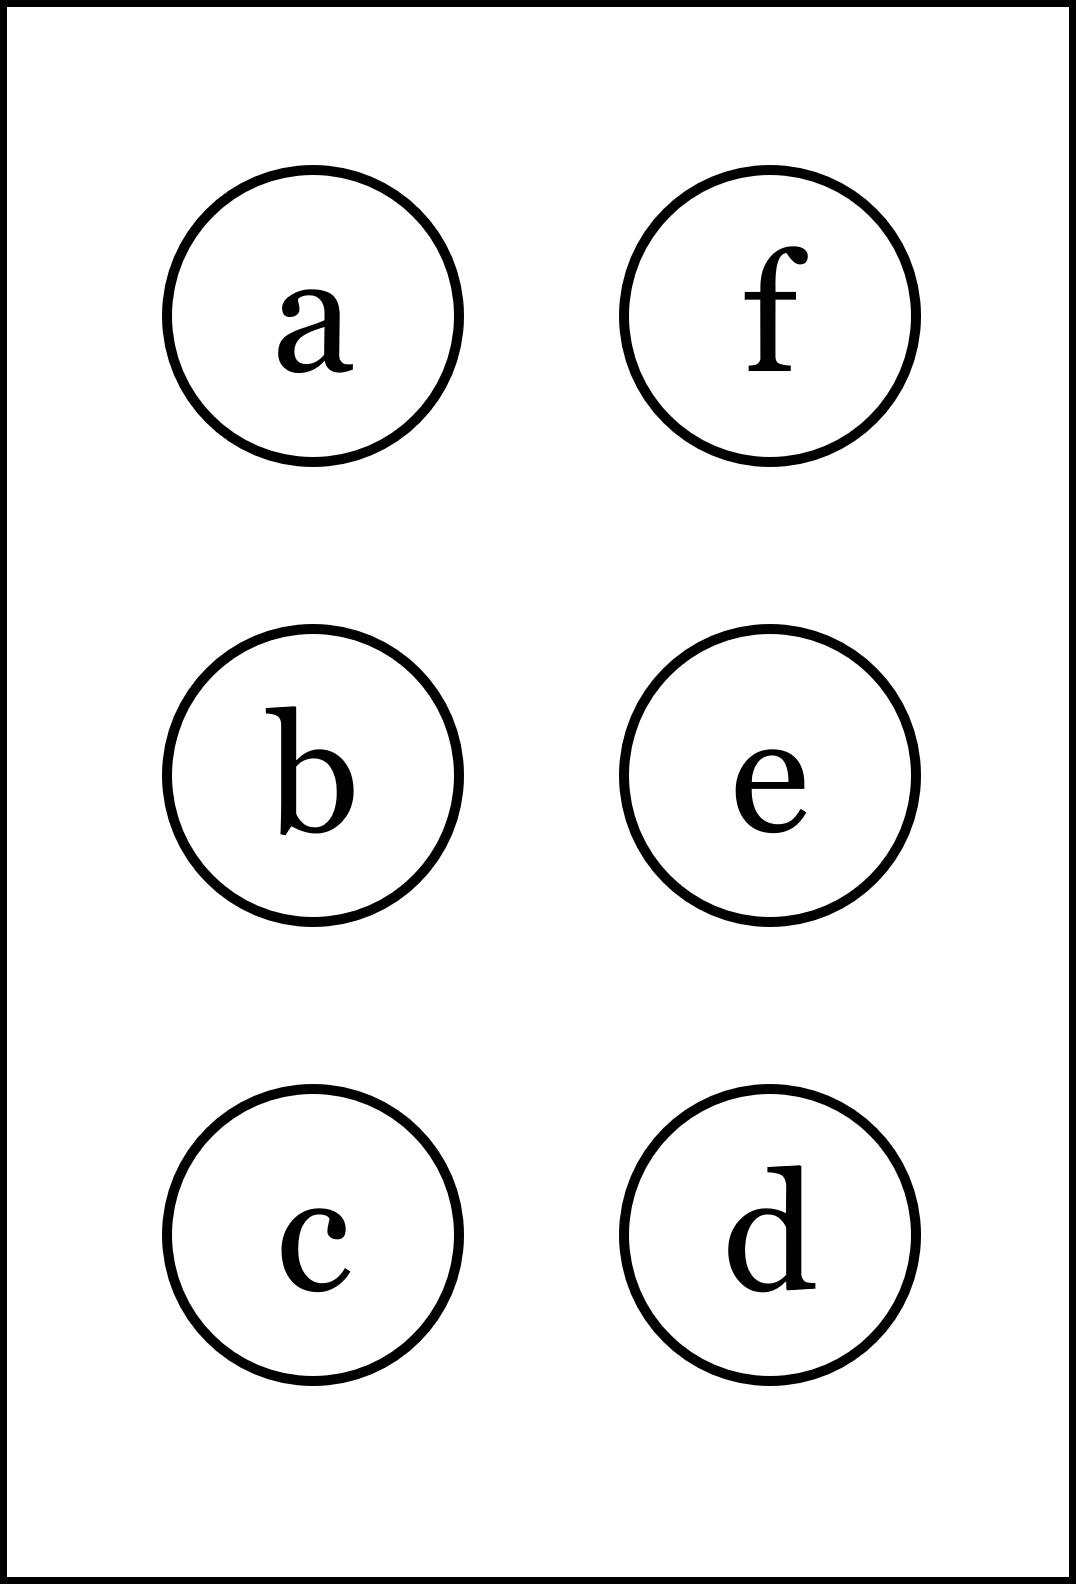
\includegraphics[height=40mm]{../images/braille.png}
{\small Písmeno Braillovej abecedy}
\end{center}
\end{minipage}
\end{center}
\end{minipage}
&
\begin{minipage}[c][104.5mm][t]{0.5\linewidth}
\begin{center}
\vspace{7mm}
{\huge Viazané extrémy, skupina \textit{Theta $\theta$} -\romannumeral4}\\[5mm]
\textit{Jméno:}\phantom{xxxxxxxxxxxxxxxxxxxxxxxxxxxxxxxxxxxxxxxxxxxxxxxxxxxxxxxxxxxxxxxxx}\\[5mm]
\begin{minipage}{0.95\linewidth}
\begin{center}
Cílem je najít \textbf{vázané extrémy} funkce $f(x,y)$ zadané v \textbf{(a)} spolu s vazbou (podmínkou). Postupuj podle krokú v \textbf{(b)} až \textbf{(f)}. Pokud se medzivýsledky shodujú s těmi za otazníky,\\tak napravo obarvi příslušející kroužek načerno. \textbf{Spolu odevzdejte výsledné slovo}.
\end{center}
\end{minipage}
\\[1mm]
\begin{minipage}{0.79\linewidth}
\begin{center}
\begin{varwidth}{\linewidth}
\begin{enumerate}
\normalsize
\item $f(x,y)=10x-24y+7 \enspace , \enspace \mathrm{vazba:} \enspace x^2+y^2=676$\quad \dotfill\; ???\;\dotfill \quad vybarvi
\item Sestav $L(\lambda,x,y)$ a spočti $\pdv{L}{x}=$\quad \dotfill\; ???\;\dotfill \quad $10+\lambda x$
\item Takisto spočti $\pdv{L}{y}=$\quad \dotfill\; ???\;\dotfill \quad $+24+2\lambda y$
\item Z podmínek $\pdv{L}{x}=0 , \pdv{L}{y}=0$ vyjádři $x,y$ v závislosti na $\lambda$.\\ \phantom{xxxxxx}Následne $x,y$ dosaď do vazbové rovnice\\ \phantom{xxxxxx}a vypočti dva výsledky pro $\lambda$.\quad \dotfill\; ???\;\dotfill \quad $\lambda_1+\lambda_2=2$
\item Pomocou $\lambda$ urč dvě dvojice pro $x,y$.\quad \dotfill\; ???\;\dotfill \quad $x_1 x_2 y_1 y_2=-2400$
\item Najdi funkční hodnoty pro oba vázané stacionární body\\ \phantom{xxxxxx}a vyber tu najvětší. $f_{\text{max}}(x,y)=$\quad \dotfill\; ???\;\dotfill \quad $682$
\end{enumerate}
\end{varwidth}
\end{center}
\end{minipage}
\begin{minipage}{0.20\linewidth}
\begin{center}
{\Huge\bfseries 4.} \\[2mm]
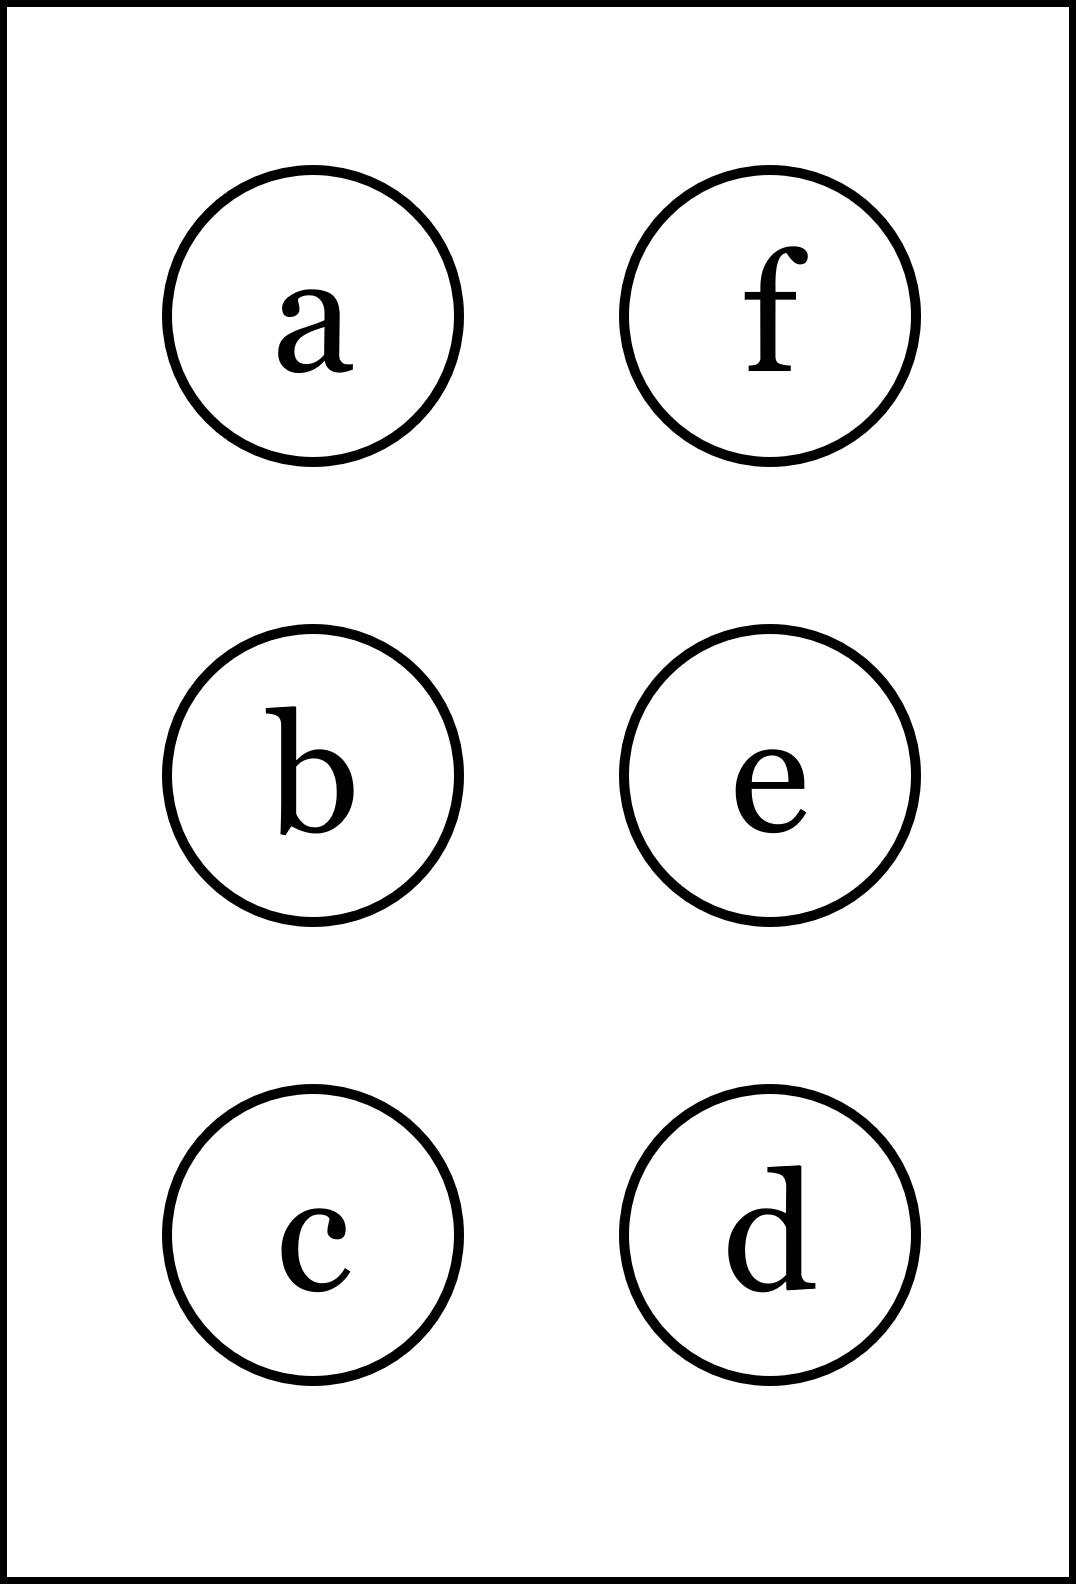
\includegraphics[height=40mm]{../images/braille.png}
{\small Písmeno Braillovej abecedy}
\end{center}
\end{minipage}
\end{center}
\end{minipage}
%
\end{tabular}
\newpage
\thispagestyle{empty}
\begin{tabular}{c:c}
\begin{minipage}[c][104.5mm][t]{0.5\linewidth}
\begin{center}
\vspace{7mm}
{\huge Viazané extrémy, skupina \textit{Iota $\iota$} -\romannumeral1}\\[5mm]
\textit{Jméno:}\phantom{xxxxxxxxxxxxxxxxxxxxxxxxxxxxxxxxxxxxxxxxxxxxxxxxxxxxxxxxxxxxxxxxx}\\[5mm]
\begin{minipage}{0.95\linewidth}
\begin{center}
Cílem je najít \textbf{vázané extrémy} funkce $f(x,y)$ zadané v \textbf{(a)} spolu s vazbou (podmínkou). Postupuj podle krokú v \textbf{(b)} až \textbf{(f)}. Pokud se medzivýsledky shodujú s těmi za otazníky,\\tak napravo obarvi příslušející kroužek načerno. \textbf{Spolu odevzdejte výsledné slovo}.
\end{center}
\end{minipage}
\\[1mm]
\begin{minipage}{0.79\linewidth}
\begin{center}
\begin{varwidth}{\linewidth}
\begin{enumerate}
\normalsize
\item $f(x,y)=3x-4y+7 \enspace , \enspace \mathrm{vazba:} \enspace x^2+y^2=25$\quad \dotfill\; ???\;\dotfill \quad nebarvi
\item Sestav $L(\lambda,x,y)$ a spočti $\pdv{L}{x}=$\quad \dotfill\; ???\;\dotfill \quad $3+2\lambda x$
\item Takisto spočti $\pdv{L}{y}=$\quad \dotfill\; ???\;\dotfill \quad $+4+2\lambda y$
\item Z podmínek $\pdv{L}{x}=0 , \pdv{L}{y}=0$ vyjádři $x,y$ v závislosti na $\lambda$.\\ \phantom{xxxxxx}Následne $x,y$ dosaď do vazbové rovnice\\ \phantom{xxxxxx}a vypočti dva výsledky pro $\lambda$.\quad \dotfill\; ???\;\dotfill \quad $\lambda_1+\lambda_2=-2$
\item Pomocou $\lambda$ urč dvě dvojice pro $x,y$.\quad \dotfill\; ???\;\dotfill \quad $x_1 x_2 y_1 y_2=-36$
\item Najdi funkční hodnoty pro oba vázané stacionární body\\ \phantom{xxxxxx}a vyber tu najvětší. $f_{\text{max}}(x,y)=$\quad \dotfill\; ???\;\dotfill \quad $32$
\end{enumerate}
\end{varwidth}
\end{center}
\end{minipage}
\begin{minipage}{0.20\linewidth}
\begin{center}
{\Huge\bfseries 1.} \\[2mm]
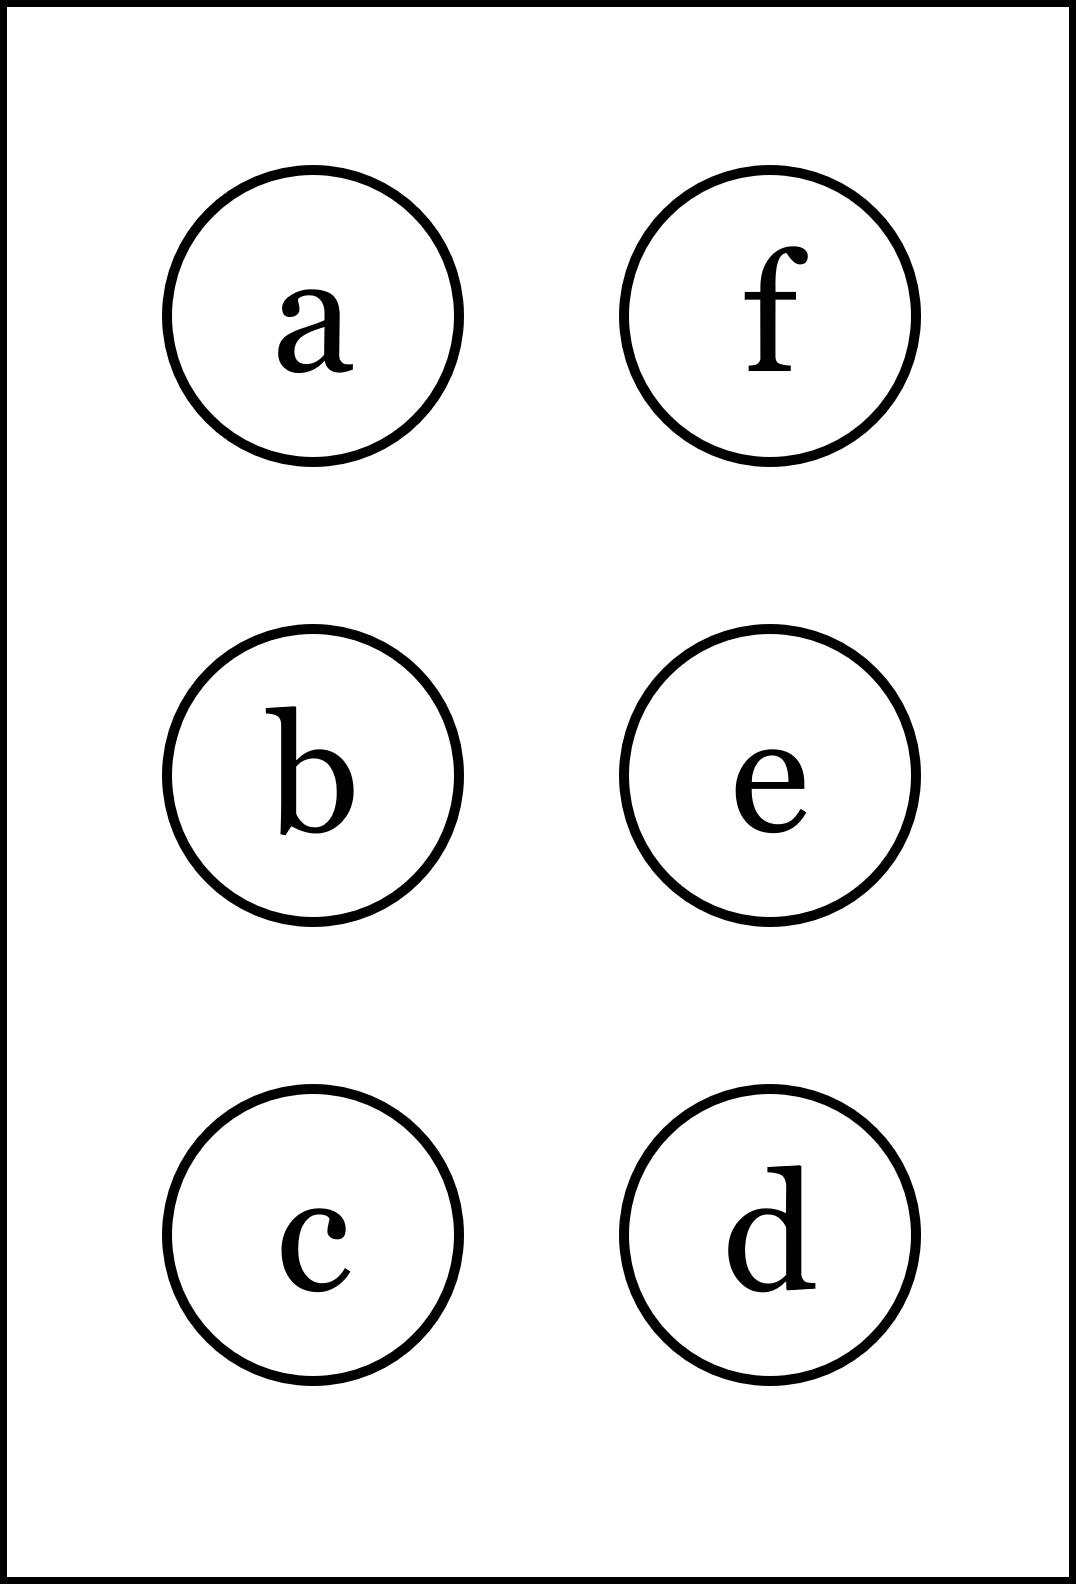
\includegraphics[height=40mm]{../images/braille.png}
{\small Písmeno Braillovej abecedy}
\end{center}
\end{minipage}
\end{center}
\end{minipage}
&
\begin{minipage}[c][104.5mm][t]{0.5\linewidth}
\begin{center}
\vspace{7mm}
{\huge Viazané extrémy, skupina \textit{Iota $\iota$} -\romannumeral2}\\[5mm]
\textit{Jméno:}\phantom{xxxxxxxxxxxxxxxxxxxxxxxxxxxxxxxxxxxxxxxxxxxxxxxxxxxxxxxxxxxxxxxxx}\\[5mm]
\begin{minipage}{0.95\linewidth}
\begin{center}
Cílem je najít \textbf{vázané extrémy} funkce $f(x,y)$ zadané v \textbf{(a)} spolu s vazbou (podmínkou). Postupuj podle krokú v \textbf{(b)} až \textbf{(f)}. Pokud se medzivýsledky shodujú s těmi za otazníky,\\tak napravo obarvi příslušející kroužek načerno. \textbf{Spolu odevzdejte výsledné slovo}.
\end{center}
\end{minipage}
\\[1mm]
\begin{minipage}{0.79\linewidth}
\begin{center}
\begin{varwidth}{\linewidth}
\begin{enumerate}
\normalsize
\item $f(x,y)=-5x+12y-4 \enspace , \enspace \mathrm{vazba:} \enspace x^2+y^2=169$\quad \dotfill\; ???\;\dotfill \quad vybarvi
\item Sestav $L(\lambda,x,y)$ a spočti $\pdv{L}{x}=$\quad \dotfill\; ???\;\dotfill \quad $-5+2\lambda x$
\item Takisto spočti $\pdv{L}{y}=$\quad \dotfill\; ???\;\dotfill \quad $-12+2\lambda y$
\item Z podmínek $\pdv{L}{x}=0 , \pdv{L}{y}=0$ vyjádři $x,y$ v závislosti na $\lambda$.\\ \phantom{xxxxxx}Následne $x,y$ dosaď do vazbové rovnice\\ \phantom{xxxxxx}a vypočti dva výsledky pro $\lambda$.\quad \dotfill\; ???\;\dotfill \quad $\lambda_1+\lambda_2=-1$
\item Pomocou $\lambda$ urč dvě dvojice pro $x,y$.\quad \dotfill\; ???\;\dotfill \quad $x_1 x_2 y_1 y_2=3600$
\item Najdi funkční hodnoty pro oba vázané stacionární body\\ \phantom{xxxxxx}a vyber tu najvětší. $f_{\text{max}}(x,y)=$\quad \dotfill\; ???\;\dotfill \quad $165$
\end{enumerate}
\end{varwidth}
\end{center}
\end{minipage}
\begin{minipage}{0.20\linewidth}
\begin{center}
{\Huge\bfseries 2.} \\[2mm]
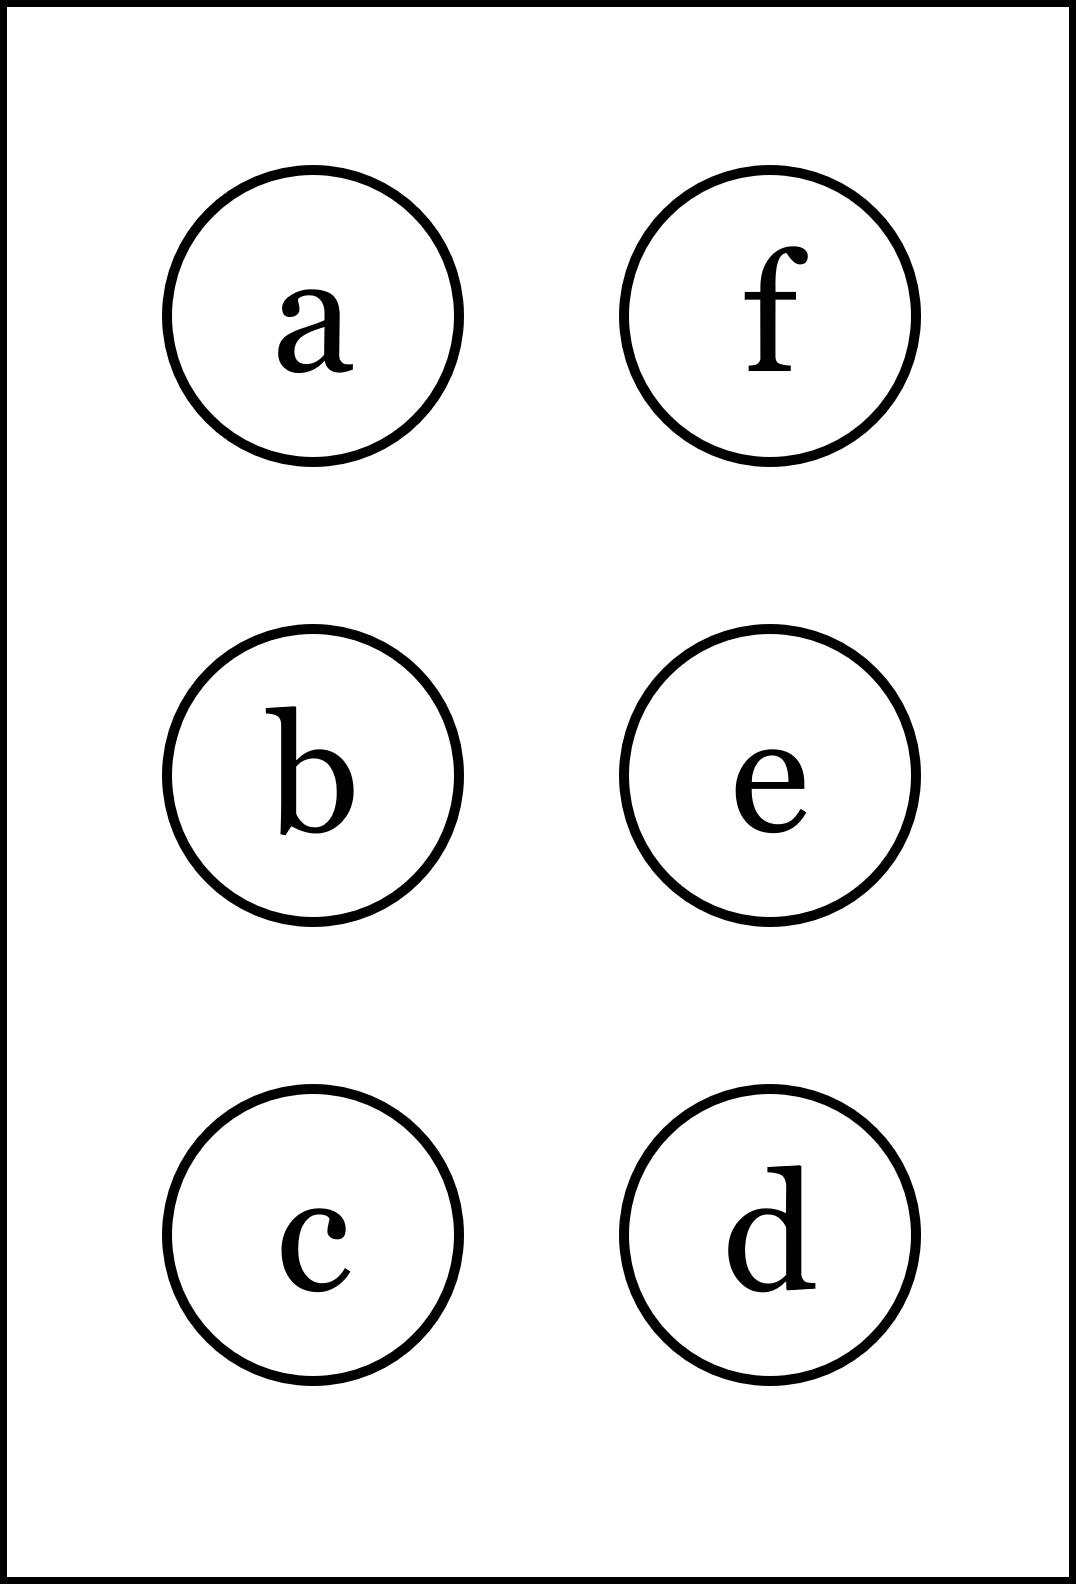
\includegraphics[height=40mm]{../images/braille.png}
{\small Písmeno Braillovej abecedy}
\end{center}
\end{minipage}
\end{center}
\end{minipage}
\\ \hdashline
\begin{minipage}[c][104.5mm][t]{0.5\linewidth}
\begin{center}
\vspace{7mm}
{\huge Viazané extrémy, skupina \textit{Iota $\iota$} -\romannumeral3}\\[5mm]
\textit{Jméno:}\phantom{xxxxxxxxxxxxxxxxxxxxxxxxxxxxxxxxxxxxxxxxxxxxxxxxxxxxxxxxxxxxxxxxx}\\[5mm]
\begin{minipage}{0.95\linewidth}
\begin{center}
Cílem je najít \textbf{vázané extrémy} funkce $f(x,y)$ zadané v \textbf{(a)} spolu s vazbou (podmínkou). Postupuj podle krokú v \textbf{(b)} až \textbf{(f)}. Pokud se medzivýsledky shodujú s těmi za otazníky,\\tak napravo obarvi příslušející kroužek načerno. \textbf{Spolu odevzdejte výsledné slovo}.
\end{center}
\end{minipage}
\\[1mm]
\begin{minipage}{0.79\linewidth}
\begin{center}
\begin{varwidth}{\linewidth}
\begin{enumerate}
\normalsize
\item $f(x,y)=-6x+8y+1 \enspace , \enspace \mathrm{vazba:} \enspace x^2+y^2=100$\quad \dotfill\; ???\;\dotfill \quad vybarvi
\item Sestav $L(\lambda,x,y)$ a spočti $\pdv{L}{x}=$\quad \dotfill\; ???\;\dotfill \quad $-6+2\lambda x$
\item Takisto spočti $\pdv{L}{y}=$\quad \dotfill\; ???\;\dotfill \quad $8+2\lambda y$
\item Z podmínek $\pdv{L}{x}=0 , \pdv{L}{y}=0$ vyjádři $x,y$ v závislosti na $\lambda$.\\ \phantom{xxxxxx}Následne $x,y$ dosaď do vazbové rovnice\\ \phantom{xxxxxx}a vypočti dva výsledky pro $\lambda$.\quad \dotfill\; ???\;\dotfill \quad $\lambda_1+\lambda_2=-1$
\item Pomocou $\lambda$ urč dvě dvojice pro $x,y$.\quad \dotfill\; ???\;\dotfill \quad $x_1 x_2 y_1 y_2=288$
\item Najdi funkční hodnoty pro oba vázané stacionární body\\ \phantom{xxxxxx}a vyber tu najvětší. $f_{\text{max}}(x,y)=$\quad \dotfill\; ???\;\dotfill \quad $100$
\end{enumerate}
\end{varwidth}
\end{center}
\end{minipage}
\begin{minipage}{0.20\linewidth}
\begin{center}
{\Huge\bfseries 3.} \\[2mm]
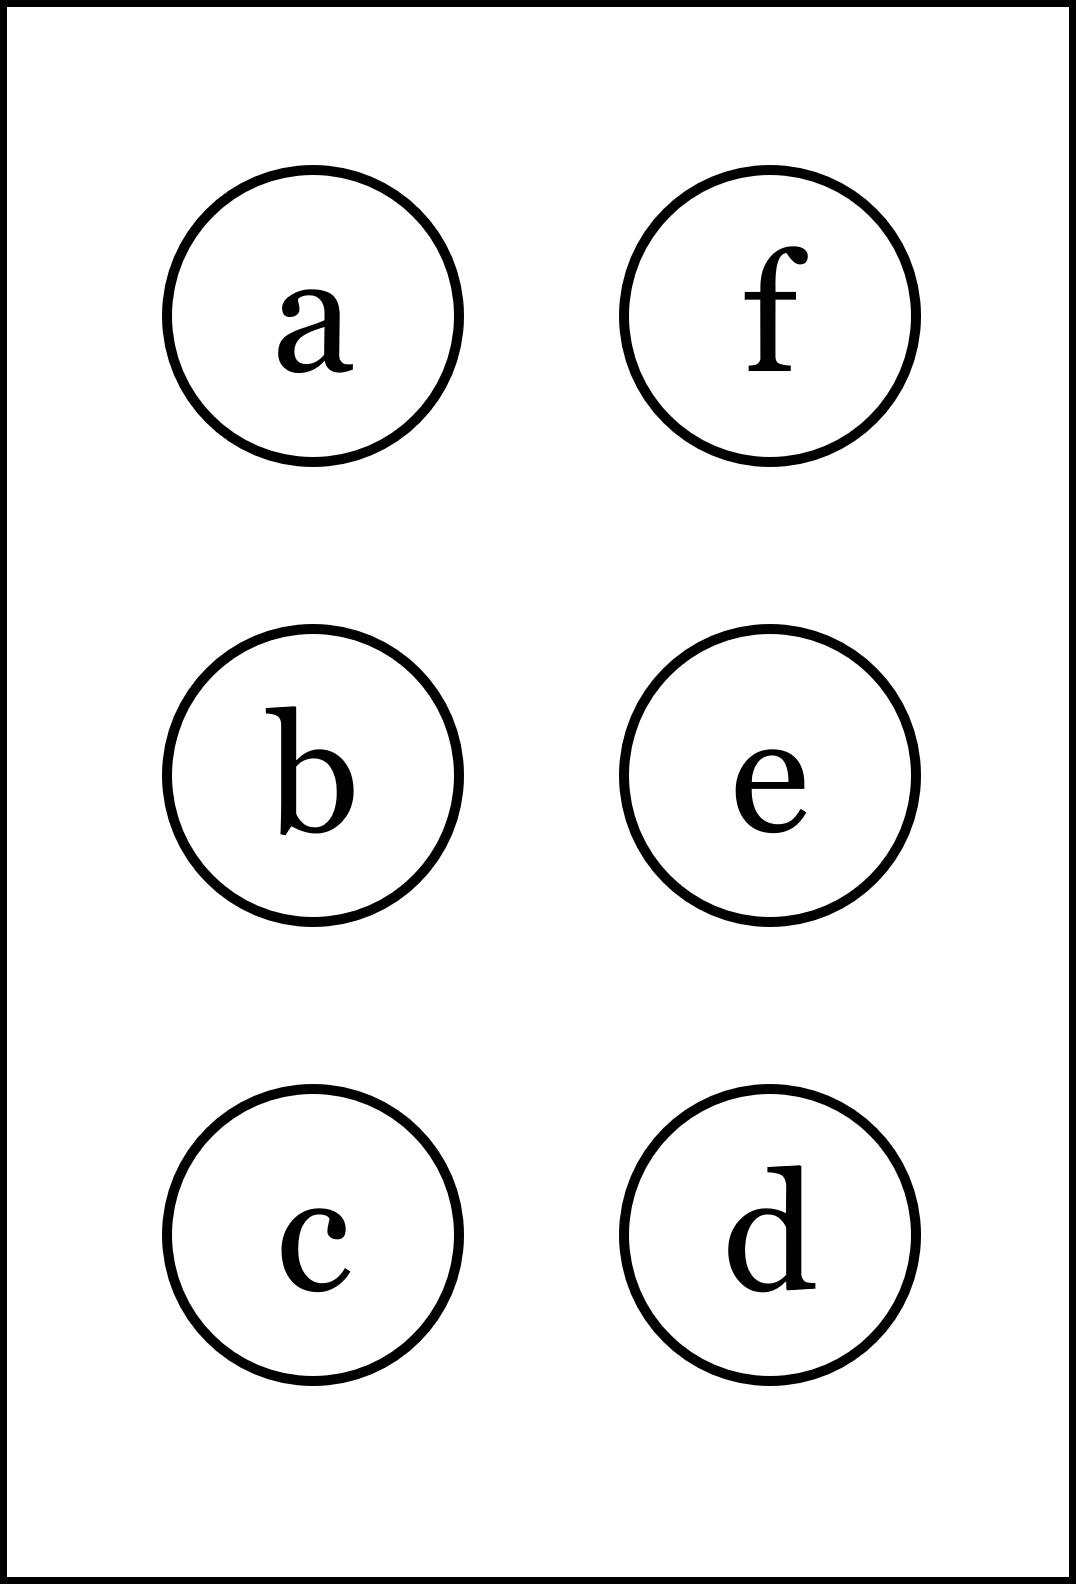
\includegraphics[height=40mm]{../images/braille.png}
{\small Písmeno Braillovej abecedy}
\end{center}
\end{minipage}
\end{center}
\end{minipage}
&
\begin{minipage}[c][104.5mm][t]{0.5\linewidth}
\begin{center}
\vspace{7mm}
{\huge Viazané extrémy, skupina \textit{Iota $\iota$} -\romannumeral4}\\[5mm]
\textit{Jméno:}\phantom{xxxxxxxxxxxxxxxxxxxxxxxxxxxxxxxxxxxxxxxxxxxxxxxxxxxxxxxxxxxxxxxxx}\\[5mm]
\begin{minipage}{0.95\linewidth}
\begin{center}
Cílem je najít \textbf{vázané extrémy} funkce $f(x,y)$ zadané v \textbf{(a)} spolu s vazbou (podmínkou). Postupuj podle krokú v \textbf{(b)} až \textbf{(f)}. Pokud se medzivýsledky shodujú s těmi za otazníky,\\tak napravo obarvi příslušející kroužek načerno. \textbf{Spolu odevzdejte výsledné slovo}.
\end{center}
\end{minipage}
\\[1mm]
\begin{minipage}{0.79\linewidth}
\begin{center}
\begin{varwidth}{\linewidth}
\begin{enumerate}
\normalsize
\item $f(x,y)=-10x+24y+2 \enspace , \enspace \mathrm{vazba:} \enspace x^2+y^2=676$\quad \dotfill\; ???\;\dotfill \quad vybarvi
\item Sestav $L(\lambda,x,y)$ a spočti $\pdv{L}{x}=$\quad \dotfill\; ???\;\dotfill \quad $-10+\lambda x$
\item Takisto spočti $\pdv{L}{y}=$\quad \dotfill\; ???\;\dotfill \quad $24+2\lambda y$
\item Z podmínek $\pdv{L}{x}=0 , \pdv{L}{y}=0$ vyjádři $x,y$ v závislosti na $\lambda$.\\ \phantom{xxxxxx}Následne $x,y$ dosaď do vazbové rovnice\\ \phantom{xxxxxx}a vypočti dva výsledky pro $\lambda$.\quad \dotfill\; ???\;\dotfill \quad $\lambda_1+\lambda_2=0$
\item Pomocou $\lambda$ urč dvě dvojice pro $x,y$.\quad \dotfill\; ???\;\dotfill \quad $x_1 x_2 y_1 y_2=2400$
\item Najdi funkční hodnoty pro oba vázané stacionární body\\ \phantom{xxxxxx}a vyber tu najvětší. $f_{\text{max}}(x,y)=$\quad \dotfill\; ???\;\dotfill \quad $677$
\end{enumerate}
\end{varwidth}
\end{center}
\end{minipage}
\begin{minipage}{0.20\linewidth}
\begin{center}
{\Huge\bfseries 4.} \\[2mm]
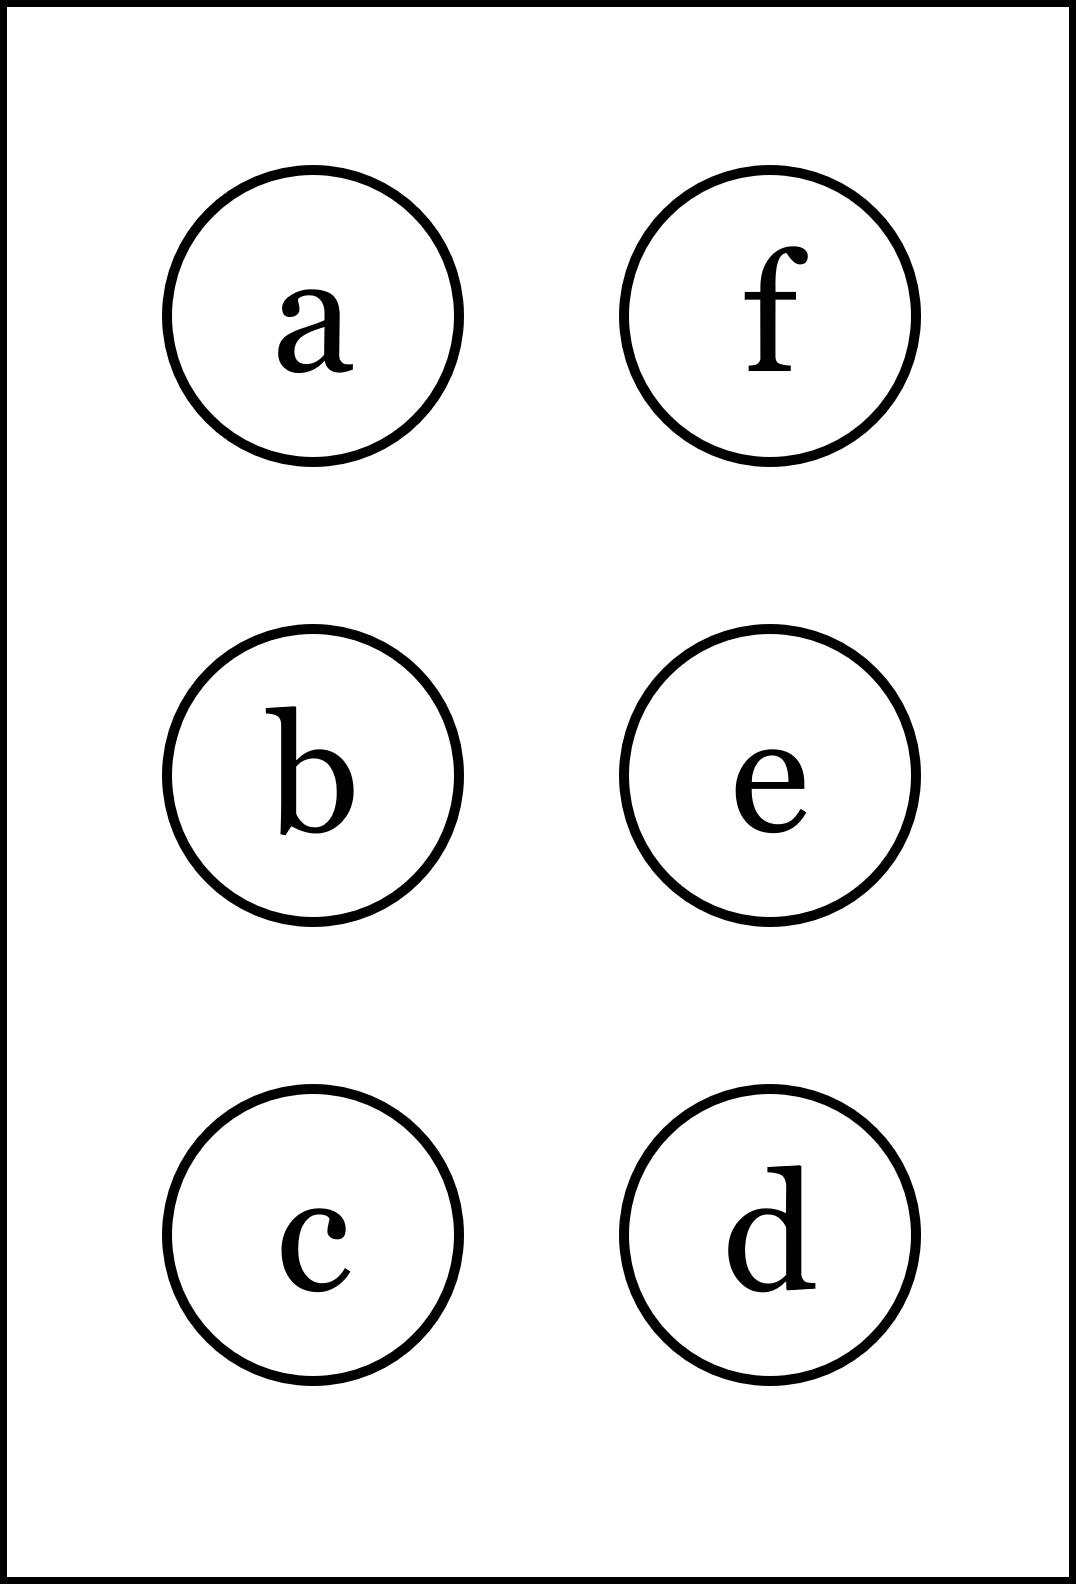
\includegraphics[height=40mm]{../images/braille.png}
{\small Písmeno Braillovej abecedy}
\end{center}
\end{minipage}
\end{center}
\end{minipage}
%
\end{tabular}
\newpage
\thispagestyle{empty}
\begin{tabular}{c:c}
\begin{minipage}[c][104.5mm][t]{0.5\linewidth}
\begin{center}
\vspace{7mm}
{\huge Viazané extrémy, skupina \textit{Kappa $\kappa$} -\romannumeral1}\\[5mm]
\textit{Jméno:}\phantom{xxxxxxxxxxxxxxxxxxxxxxxxxxxxxxxxxxxxxxxxxxxxxxxxxxxxxxxxxxxxxxxxx}\\[5mm]
\begin{minipage}{0.95\linewidth}
\begin{center}
Cílem je najít \textbf{vázané extrémy} funkce $f(x,y)$ zadané v \textbf{(a)} spolu s vazbou (podmínkou). Postupuj podle krokú v \textbf{(b)} až \textbf{(f)}. Pokud se medzivýsledky shodujú s těmi za otazníky,\\tak napravo obarvi příslušející kroužek načerno. \textbf{Spolu odevzdejte výsledné slovo}.
\end{center}
\end{minipage}
\\[1mm]
\begin{minipage}{0.79\linewidth}
\begin{center}
\begin{varwidth}{\linewidth}
\begin{enumerate}
\normalsize
\item $f(x,y)=-3x+4y+2 \enspace , \enspace \mathrm{vazba:} \enspace x^2+y^2=25$\quad \dotfill\; ???\;\dotfill \quad vybarvi
\item Sestav $L(\lambda,x,y)$ a spočti $\pdv{L}{x}=$\quad \dotfill\; ???\;\dotfill \quad $-3+\lambda x$
\item Takisto spočti $\pdv{L}{y}=$\quad \dotfill\; ???\;\dotfill \quad $-4+2\lambda y$
\item Z podmínek $\pdv{L}{x}=0 , \pdv{L}{y}=0$ vyjádři $x,y$ v závislosti na $\lambda$.\\ \phantom{xxxxxx}Následne $x,y$ dosaď do vazbové rovnice\\ \phantom{xxxxxx}a vypočti dva výsledky pro $\lambda$.\quad \dotfill\; ???\;\dotfill \quad $\lambda_1+\lambda_2=1$
\item Pomocou $\lambda$ urč dvě dvojice pro $x,y$.\quad \dotfill\; ???\;\dotfill \quad $x_1 x_2 y_1 y_2=36$
\item Najdi funkční hodnoty pro oba vázané stacionární body\\ \phantom{xxxxxx}a vyber tu najvětší. $f_{\text{max}}(x,y)=$\quad \dotfill\; ???\;\dotfill \quad $27$
\end{enumerate}
\end{varwidth}
\end{center}
\end{minipage}
\begin{minipage}{0.20\linewidth}
\begin{center}
{\Huge\bfseries 1.} \\[2mm]
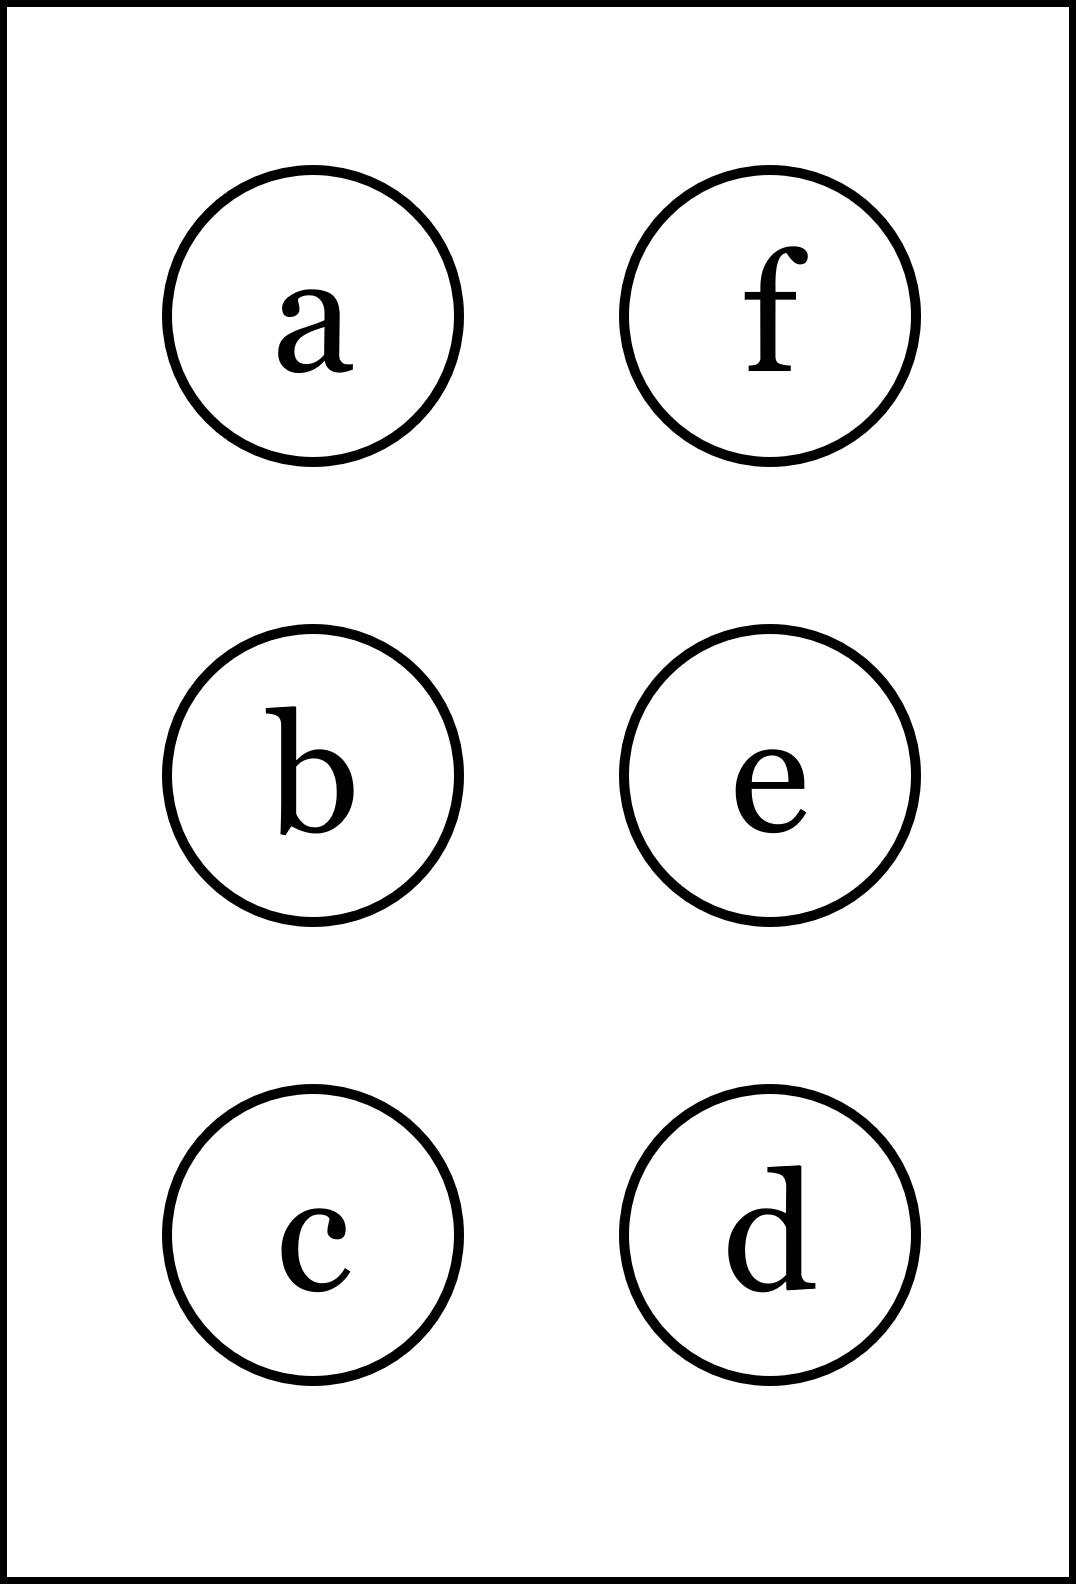
\includegraphics[height=40mm]{../images/braille.png}
{\small Písmeno Braillovej abecedy}
\end{center}
\end{minipage}
\end{center}
\end{minipage}
&
\begin{minipage}[c][104.5mm][t]{0.5\linewidth}
\begin{center}
\vspace{7mm}
{\huge Viazané extrémy, skupina \textit{Kappa $\kappa$} -\romannumeral2}\\[5mm]
\textit{Jméno:}\phantom{xxxxxxxxxxxxxxxxxxxxxxxxxxxxxxxxxxxxxxxxxxxxxxxxxxxxxxxxxxxxxxxxx}\\[5mm]
\begin{minipage}{0.95\linewidth}
\begin{center}
Cílem je najít \textbf{vázané extrémy} funkce $f(x,y)$ zadané v \textbf{(a)} spolu s vazbou (podmínkou). Postupuj podle krokú v \textbf{(b)} až \textbf{(f)}. Pokud se medzivýsledky shodujú s těmi za otazníky,\\tak napravo obarvi příslušející kroužek načerno. \textbf{Spolu odevzdejte výsledné slovo}.
\end{center}
\end{minipage}
\\[1mm]
\begin{minipage}{0.79\linewidth}
\begin{center}
\begin{varwidth}{\linewidth}
\begin{enumerate}
\normalsize
\item $f(x,y)=-5x+12y+6 \enspace , \enspace \mathrm{vazba:} \enspace x^2+y^2=169$\quad \dotfill\; ???\;\dotfill \quad vybarvi
\item Sestav $L(\lambda,x,y)$ a spočti $\pdv{L}{x}=$\quad \dotfill\; ???\;\dotfill \quad $-5+\lambda x$
\item Takisto spočti $\pdv{L}{y}=$\quad \dotfill\; ???\;\dotfill \quad $12+2\lambda y$
\item Z podmínek $\pdv{L}{x}=0 , \pdv{L}{y}=0$ vyjádři $x,y$ v závislosti na $\lambda$.\\ \phantom{xxxxxx}Následne $x,y$ dosaď do vazbové rovnice\\ \phantom{xxxxxx}a vypočti dva výsledky pro $\lambda$.\quad \dotfill\; ???\;\dotfill \quad $\lambda_1+\lambda_2=2$
\item Pomocou $\lambda$ urč dvě dvojice pro $x,y$.\quad \dotfill\; ???\;\dotfill \quad $x_1 x_2 y_1 y_2=3600$
\item Najdi funkční hodnoty pro oba vázané stacionární body\\ \phantom{xxxxxx}a vyber tu najvětší. $f_{\text{max}}(x,y)=$\quad \dotfill\; ???\;\dotfill \quad $174$
\end{enumerate}
\end{varwidth}
\end{center}
\end{minipage}
\begin{minipage}{0.20\linewidth}
\begin{center}
{\Huge\bfseries 2.} \\[2mm]
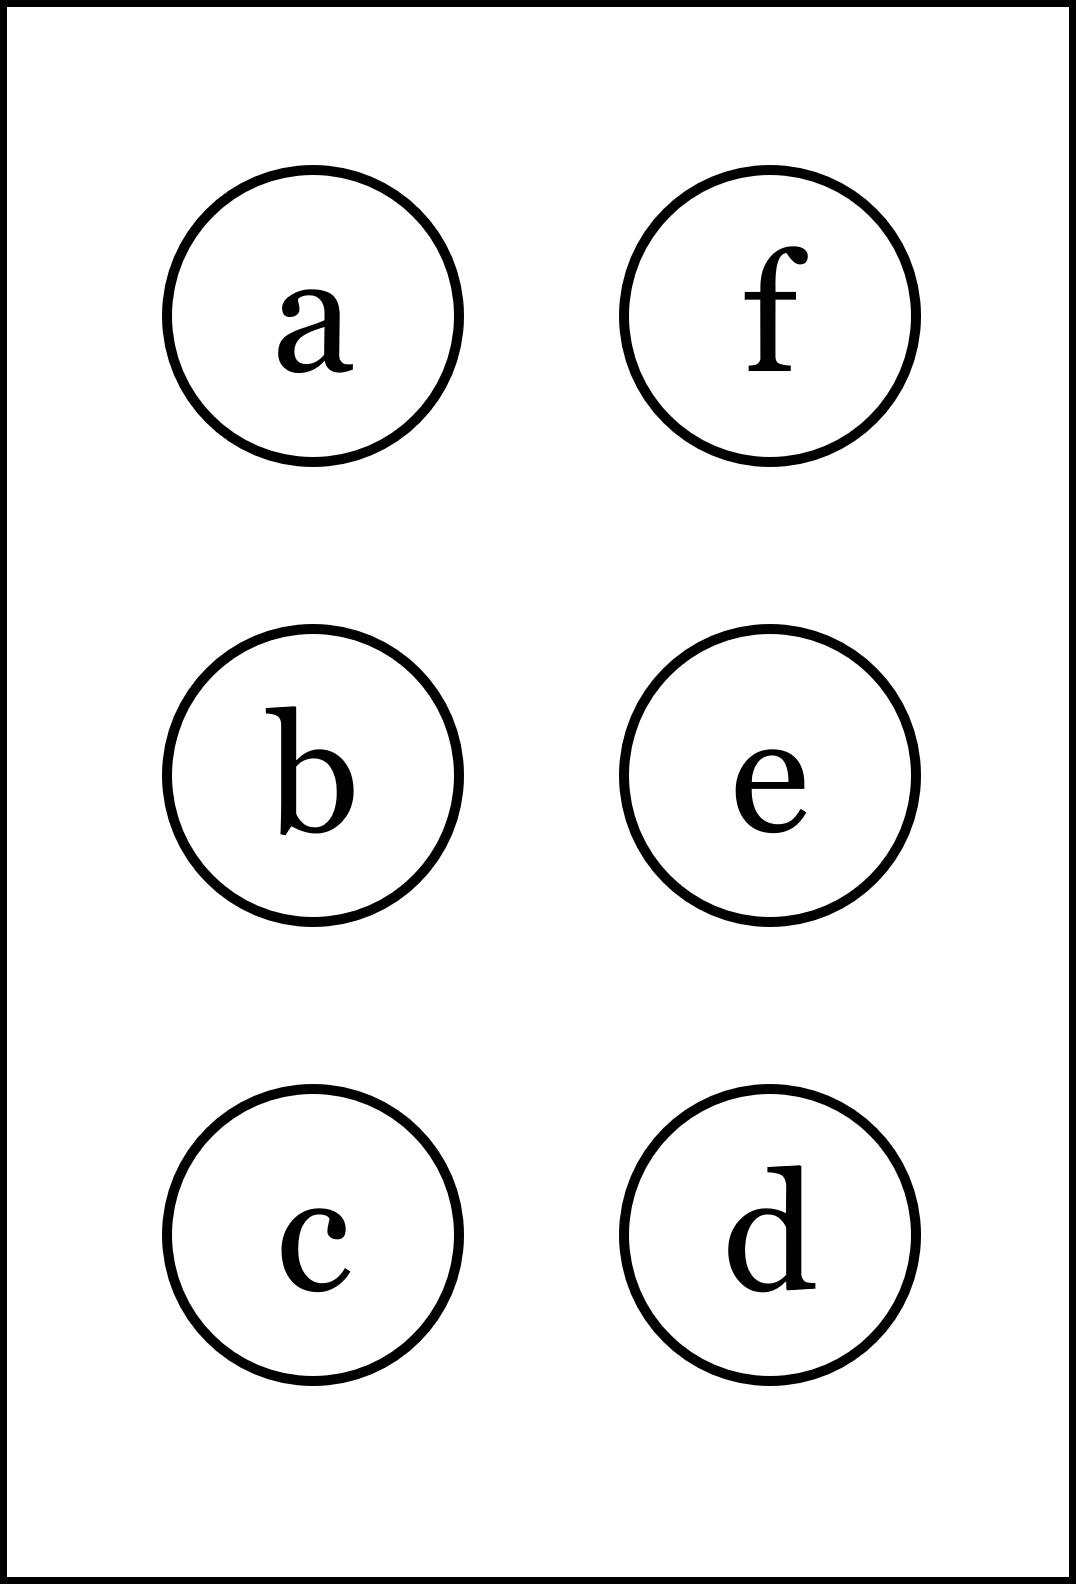
\includegraphics[height=40mm]{../images/braille.png}
{\small Písmeno Braillovej abecedy}
\end{center}
\end{minipage}
\end{center}
\end{minipage}
\\ \hdashline
\begin{minipage}[c][104.5mm][t]{0.5\linewidth}
\begin{center}
\vspace{7mm}
{\huge Viazané extrémy, skupina \textit{Kappa $\kappa$} -\romannumeral3}\\[5mm]
\textit{Jméno:}\phantom{xxxxxxxxxxxxxxxxxxxxxxxxxxxxxxxxxxxxxxxxxxxxxxxxxxxxxxxxxxxxxxxxx}\\[5mm]
\begin{minipage}{0.95\linewidth}
\begin{center}
Cílem je najít \textbf{vázané extrémy} funkce $f(x,y)$ zadané v \textbf{(a)} spolu s vazbou (podmínkou). Postupuj podle krokú v \textbf{(b)} až \textbf{(f)}. Pokud se medzivýsledky shodujú s těmi za otazníky,\\tak napravo obarvi příslušející kroužek načerno. \textbf{Spolu odevzdejte výsledné slovo}.
\end{center}
\end{minipage}
\\[1mm]
\begin{minipage}{0.79\linewidth}
\begin{center}
\begin{varwidth}{\linewidth}
\begin{enumerate}
\normalsize
\item $f(x,y)=6x+8y+1 \enspace , \enspace \mathrm{vazba:} \enspace x^2+y^2=100$\quad \dotfill\; ???\;\dotfill \quad vybarvi
\item Sestav $L(\lambda,x,y)$ a spočti $\pdv{L}{x}=$\quad \dotfill\; ???\;\dotfill \quad $6+2\lambda x$
\item Takisto spočti $\pdv{L}{y}=$\quad \dotfill\; ???\;\dotfill \quad $8+2\lambda y$
\item Z podmínek $\pdv{L}{x}=0 , \pdv{L}{y}=0$ vyjádři $x,y$ v závislosti na $\lambda$.\\ \phantom{xxxxxx}Následne $x,y$ dosaď do vazbové rovnice\\ \phantom{xxxxxx}a vypočti dva výsledky pro $\lambda$.\quad \dotfill\; ???\;\dotfill \quad $\lambda_1+\lambda_2=-2$
\item Pomocou $\lambda$ urč dvě dvojice pro $x,y$.\quad \dotfill\; ???\;\dotfill \quad $x_1 x_2 y_1 y_2=288$
\item Najdi funkční hodnoty pro oba vázané stacionární body\\ \phantom{xxxxxx}a vyber tu najvětší. $f_{\text{max}}(x,y)=$\quad \dotfill\; ???\;\dotfill \quad $101$
\end{enumerate}
\end{varwidth}
\end{center}
\end{minipage}
\begin{minipage}{0.20\linewidth}
\begin{center}
{\Huge\bfseries 3.} \\[2mm]
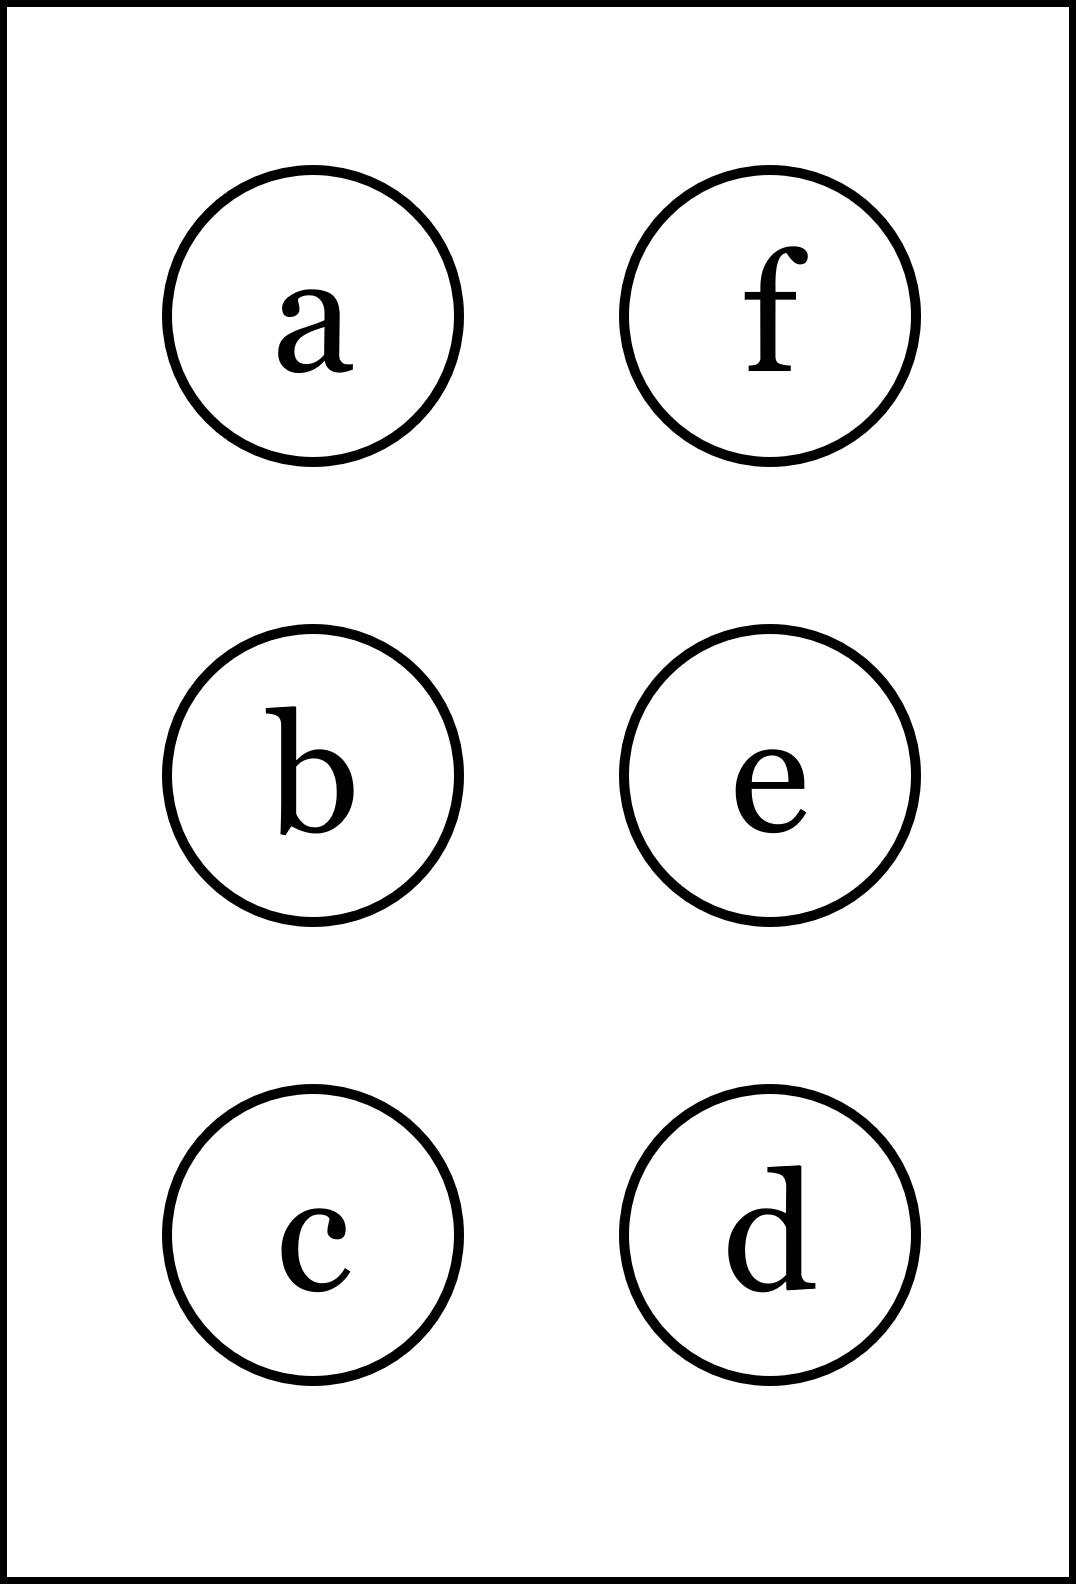
\includegraphics[height=40mm]{../images/braille.png}
{\small Písmeno Braillovej abecedy}
\end{center}
\end{minipage}
\end{center}
\end{minipage}
&
\begin{minipage}[c][104.5mm][t]{0.5\linewidth}
\begin{center}
\vspace{7mm}
{\huge Viazané extrémy, skupina \textit{Kappa $\kappa$} -\romannumeral4}\\[5mm]
\textit{Jméno:}\phantom{xxxxxxxxxxxxxxxxxxxxxxxxxxxxxxxxxxxxxxxxxxxxxxxxxxxxxxxxxxxxxxxxx}\\[5mm]
\begin{minipage}{0.95\linewidth}
\begin{center}
Cílem je najít \textbf{vázané extrémy} funkce $f(x,y)$ zadané v \textbf{(a)} spolu s vazbou (podmínkou). Postupuj podle krokú v \textbf{(b)} až \textbf{(f)}. Pokud se medzivýsledky shodujú s těmi za otazníky,\\tak napravo obarvi příslušející kroužek načerno. \textbf{Spolu odevzdejte výsledné slovo}.
\end{center}
\end{minipage}
\\[1mm]
\begin{minipage}{0.79\linewidth}
\begin{center}
\begin{varwidth}{\linewidth}
\begin{enumerate}
\normalsize
\item $f(x,y)=10x+24y-2 \enspace , \enspace \mathrm{vazba:} \enspace x^2+y^2=676$\quad \dotfill\; ???\;\dotfill \quad vybarvi
\item Sestav $L(\lambda,x,y)$ a spočti $\pdv{L}{x}=$\quad \dotfill\; ???\;\dotfill \quad $10+\lambda x$
\item Takisto spočti $\pdv{L}{y}=$\quad \dotfill\; ???\;\dotfill \quad $24+2\lambda y$
\item Z podmínek $\pdv{L}{x}=0 , \pdv{L}{y}=0$ vyjádři $x,y$ v závislosti na $\lambda$.\\ \phantom{xxxxxx}Následne $x,y$ dosaď do vazbové rovnice\\ \phantom{xxxxxx}a vypočti dva výsledky pro $\lambda$.\quad \dotfill\; ???\;\dotfill \quad $\lambda_1+\lambda_2=0$
\item Pomocou $\lambda$ urč dvě dvojice pro $x,y$.\quad \dotfill\; ???\;\dotfill \quad $x_1 x_2 y_1 y_2=57600$
\item Najdi funkční hodnoty pro oba vázané stacionární body\\ \phantom{xxxxxx}a vyber tu najvětší. $f_{\text{max}}(x,y)=$\quad \dotfill\; ???\;\dotfill \quad $674$
\end{enumerate}
\end{varwidth}
\end{center}
\end{minipage}
\begin{minipage}{0.20\linewidth}
\begin{center}
{\Huge\bfseries 4.} \\[2mm]
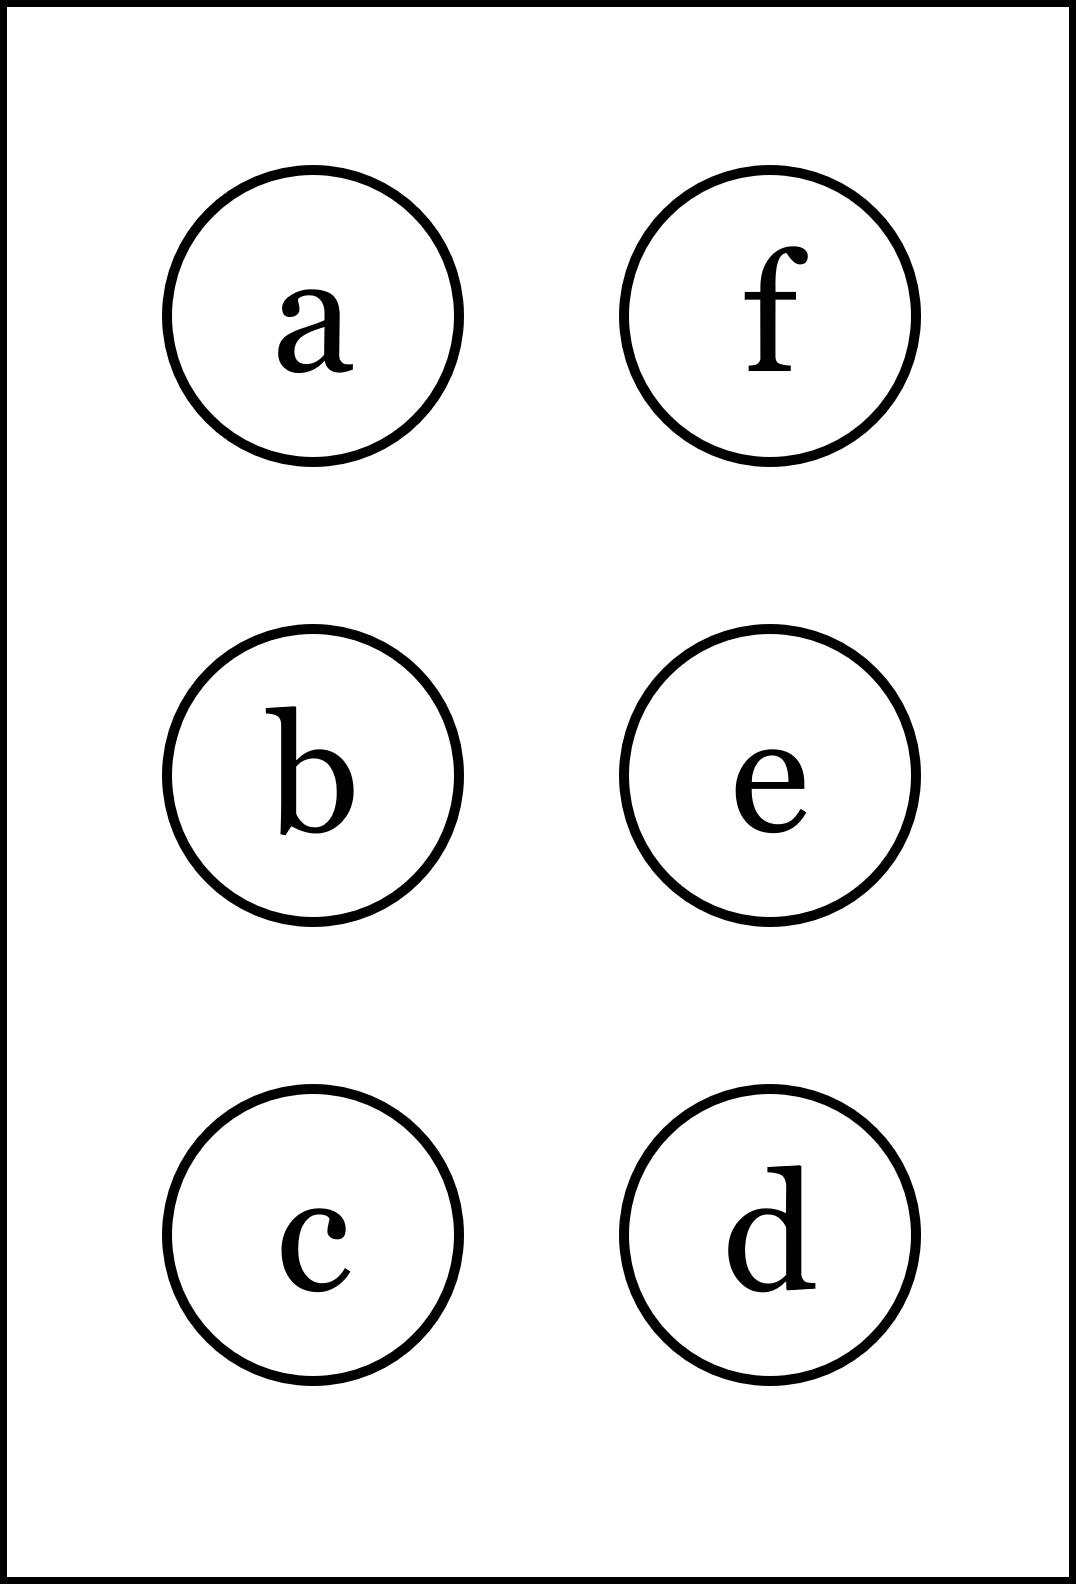
\includegraphics[height=40mm]{../images/braille.png}
{\small Písmeno Braillovej abecedy}
\end{center}
\end{minipage}
\end{center}
\end{minipage}
%
\end{tabular}
\newpage
\thispagestyle{empty}
\begin{tabular}{c:c}
\begin{minipage}[c][104.5mm][t]{0.5\linewidth}
\begin{center}
\vspace{7mm}
{\huge Viazané extrémy, skupina \textit{Lambda $\lambda$} -\romannumeral1}\\[5mm]
\textit{Jméno:}\phantom{xxxxxxxxxxxxxxxxxxxxxxxxxxxxxxxxxxxxxxxxxxxxxxxxxxxxxxxxxxxxxxxxx}\\[5mm]
\begin{minipage}{0.95\linewidth}
\begin{center}
Cílem je najít \textbf{vázané extrémy} funkce $f(x,y)$ zadané v \textbf{(a)} spolu s vazbou (podmínkou). Postupuj podle krokú v \textbf{(b)} až \textbf{(f)}. Pokud se medzivýsledky shodujú s těmi za otazníky,\\tak napravo obarvi příslušející kroužek načerno. \textbf{Spolu odevzdejte výsledné slovo}.
\end{center}
\end{minipage}
\\[1mm]
\begin{minipage}{0.79\linewidth}
\begin{center}
\begin{varwidth}{\linewidth}
\begin{enumerate}
\normalsize
\item $f(x,y)=3x+4y+4 \enspace , \enspace \mathrm{vazba:} \enspace x^2+y^2=25$\quad \dotfill\; ???\;\dotfill \quad vybarvi
\item Sestav $L(\lambda,x,y)$ a spočti $\pdv{L}{x}=$\quad \dotfill\; ???\;\dotfill \quad $3+\lambda x$
\item Takisto spočti $\pdv{L}{y}=$\quad \dotfill\; ???\;\dotfill \quad $-4+2\lambda y$
\item Z podmínek $\pdv{L}{x}=0 , \pdv{L}{y}=0$ vyjádři $x,y$ v závislosti na $\lambda$.\\ \phantom{xxxxxx}Následne $x,y$ dosaď do vazbové rovnice\\ \phantom{xxxxxx}a vypočti dva výsledky pro $\lambda$.\quad \dotfill\; ???\;\dotfill \quad $\lambda_1+\lambda_2=0$
\item Pomocou $\lambda$ urč dvě dvojice pro $x,y$.\quad \dotfill\; ???\;\dotfill \quad $x_1 x_2 y_1 y_2=36$
\item Najdi funkční hodnoty pro oba vázané stacionární body\\ \phantom{xxxxxx}a vyber tu najvětší. $f_{\text{max}}(x,y)=$\quad \dotfill\; ???\;\dotfill \quad $29$
\end{enumerate}
\end{varwidth}
\end{center}
\end{minipage}
\begin{minipage}{0.20\linewidth}
\begin{center}
{\Huge\bfseries 1.} \\[2mm]
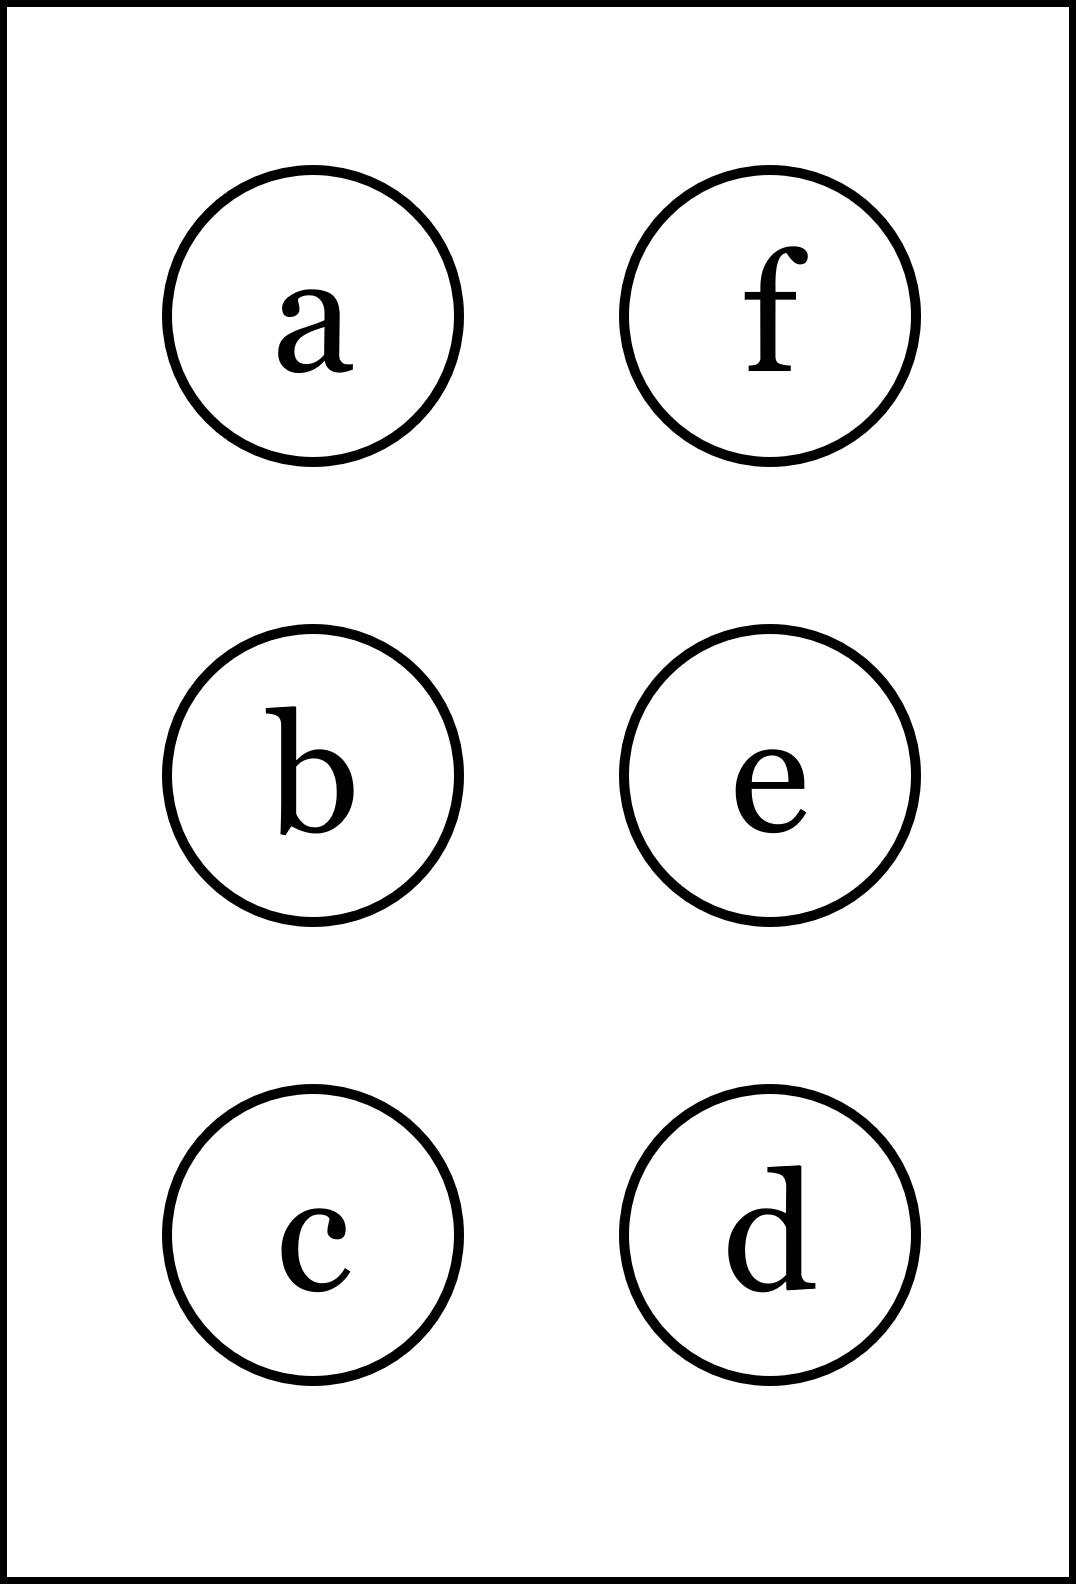
\includegraphics[height=40mm]{../images/braille.png}
{\small Písmeno Braillovej abecedy}
\end{center}
\end{minipage}
\end{center}
\end{minipage}
&
\begin{minipage}[c][104.5mm][t]{0.5\linewidth}
\begin{center}
\vspace{7mm}
{\huge Viazané extrémy, skupina \textit{Lambda $\lambda$} -\romannumeral2}\\[5mm]
\textit{Jméno:}\phantom{xxxxxxxxxxxxxxxxxxxxxxxxxxxxxxxxxxxxxxxxxxxxxxxxxxxxxxxxxxxxxxxxx}\\[5mm]
\begin{minipage}{0.95\linewidth}
\begin{center}
Cílem je najít \textbf{vázané extrémy} funkce $f(x,y)$ zadané v \textbf{(a)} spolu s vazbou (podmínkou). Postupuj podle krokú v \textbf{(b)} až \textbf{(f)}. Pokud se medzivýsledky shodujú s těmi za otazníky,\\tak napravo obarvi příslušející kroužek načerno. \textbf{Spolu odevzdejte výsledné slovo}.
\end{center}
\end{minipage}
\\[1mm]
\begin{minipage}{0.79\linewidth}
\begin{center}
\begin{varwidth}{\linewidth}
\begin{enumerate}
\normalsize
\item $f(x,y)=5x+12y-6 \enspace , \enspace \mathrm{vazba:} \enspace x^2+y^2=169$\quad \dotfill\; ???\;\dotfill \quad vybarvi
\item Sestav $L(\lambda,x,y)$ a spočti $\pdv{L}{x}=$\quad \dotfill\; ???\;\dotfill \quad $5+\lambda x$
\item Takisto spočti $\pdv{L}{y}=$\quad \dotfill\; ???\;\dotfill \quad $-12+2\lambda y$
\item Z podmínek $\pdv{L}{x}=0 , \pdv{L}{y}=0$ vyjádři $x,y$ v závislosti na $\lambda$.\\ \phantom{xxxxxx}Následne $x,y$ dosaď do vazbové rovnice\\ \phantom{xxxxxx}a vypočti dva výsledky pro $\lambda$.\quad \dotfill\; ???\;\dotfill \quad $\lambda_1+\lambda_2=-2$
\item Pomocou $\lambda$ urč dvě dvojice pro $x,y$.\quad \dotfill\; ???\;\dotfill \quad $x_1 x_2 y_1 y_2=3600$
\item Najdi funkční hodnoty pro oba vázané stacionární body\\ \phantom{xxxxxx}a vyber tu najvětší. $f_{\text{max}}(x,y)=$\quad \dotfill\; ???\;\dotfill \quad $162$
\end{enumerate}
\end{varwidth}
\end{center}
\end{minipage}
\begin{minipage}{0.20\linewidth}
\begin{center}
{\Huge\bfseries 2.} \\[2mm]
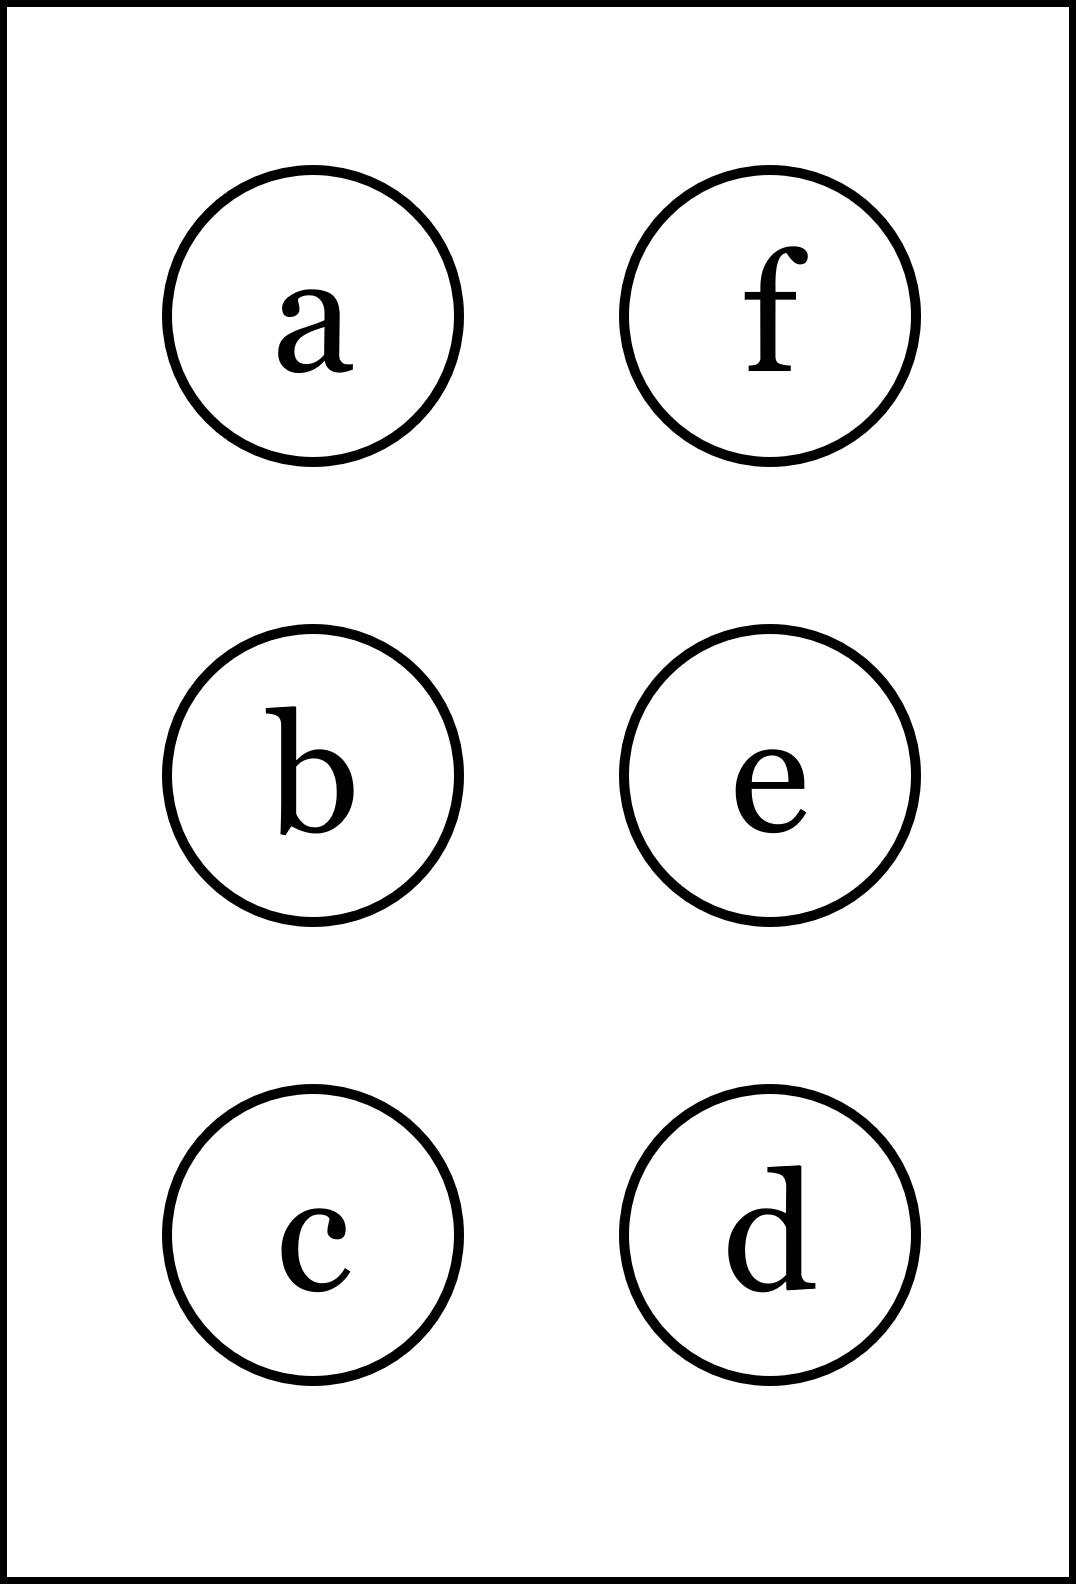
\includegraphics[height=40mm]{../images/braille.png}
{\small Písmeno Braillovej abecedy}
\end{center}
\end{minipage}
\end{center}
\end{minipage}
\\ \hdashline
\begin{minipage}[c][104.5mm][t]{0.5\linewidth}
\begin{center}
\vspace{7mm}
{\huge Viazané extrémy, skupina \textit{Lambda $\lambda$} -\romannumeral3}\\[5mm]
\textit{Jméno:}\phantom{xxxxxxxxxxxxxxxxxxxxxxxxxxxxxxxxxxxxxxxxxxxxxxxxxxxxxxxxxxxxxxxxx}\\[5mm]
\begin{minipage}{0.95\linewidth}
\begin{center}
Cílem je najít \textbf{vázané extrémy} funkce $f(x,y)$ zadané v \textbf{(a)} spolu s vazbou (podmínkou). Postupuj podle krokú v \textbf{(b)} až \textbf{(f)}. Pokud se medzivýsledky shodujú s těmi za otazníky,\\tak napravo obarvi příslušející kroužek načerno. \textbf{Spolu odevzdejte výsledné slovo}.
\end{center}
\end{minipage}
\\[1mm]
\begin{minipage}{0.79\linewidth}
\begin{center}
\begin{varwidth}{\linewidth}
\begin{enumerate}
\normalsize
\item $f(x,y)=-6x+8y-6 \enspace , \enspace \mathrm{vazba:} \enspace x^2+y^2=100$\quad \dotfill\; ???\;\dotfill \quad nebarvi
\item Sestav $L(\lambda,x,y)$ a spočti $\pdv{L}{x}=$\quad \dotfill\; ???\;\dotfill \quad $-6+2\lambda x$
\item Takisto spočti $\pdv{L}{y}=$\quad \dotfill\; ???\;\dotfill \quad $8+2\lambda y$
\item Z podmínek $\pdv{L}{x}=0 , \pdv{L}{y}=0$ vyjádři $x,y$ v závislosti na $\lambda$.\\ \phantom{xxxxxx}Následne $x,y$ dosaď do vazbové rovnice\\ \phantom{xxxxxx}a vypočti dva výsledky pro $\lambda$.\quad \dotfill\; ???\;\dotfill \quad $\lambda_1+\lambda_2=1$
\item Pomocou $\lambda$ urč dvě dvojice pro $x,y$.\quad \dotfill\; ???\;\dotfill \quad $x_1 x_2 y_1 y_2=288$
\item Najdi funkční hodnoty pro oba vázané stacionární body\\ \phantom{xxxxxx}a vyber tu najvětší. $f_{\text{max}}(x,y)=$\quad \dotfill\; ???\;\dotfill \quad $94$
\end{enumerate}
\end{varwidth}
\end{center}
\end{minipage}
\begin{minipage}{0.20\linewidth}
\begin{center}
{\Huge\bfseries 3.} \\[2mm]
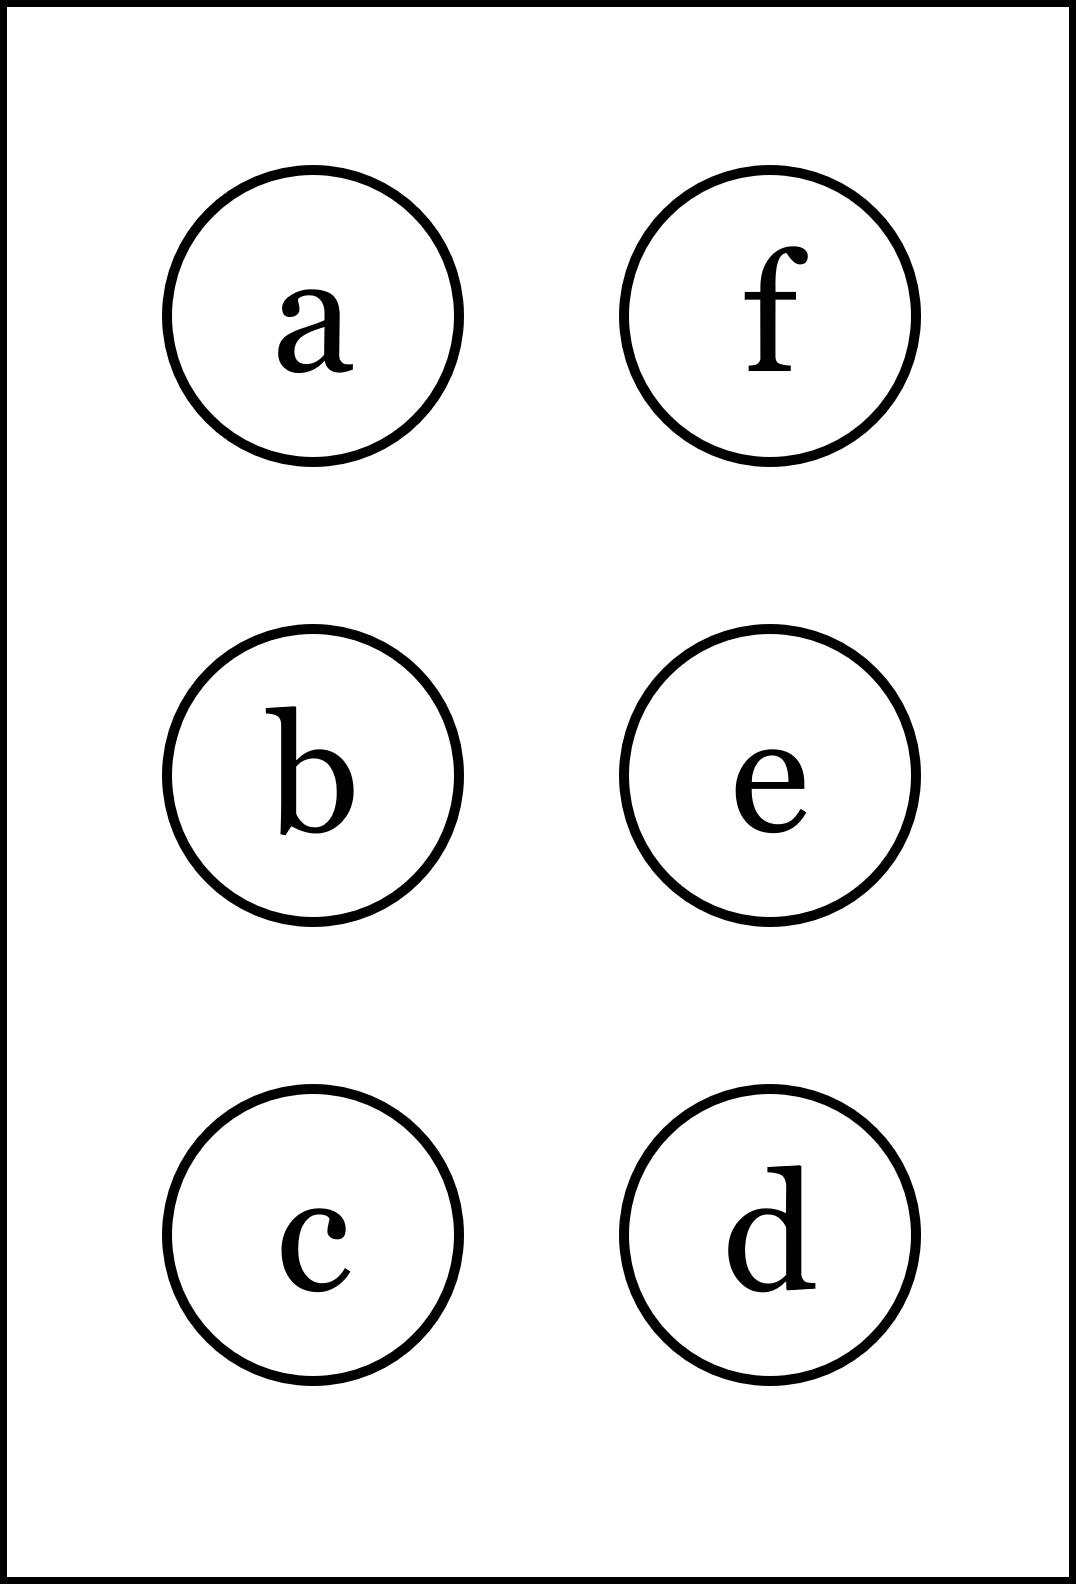
\includegraphics[height=40mm]{../images/braille.png}
{\small Písmeno Braillovej abecedy}
\end{center}
\end{minipage}
\end{center}
\end{minipage}
&
\begin{minipage}[c][104.5mm][t]{0.5\linewidth}
\begin{center}
\vspace{7mm}
{\huge Viazané extrémy, skupina \textit{Lambda $\lambda$} -\romannumeral4}\\[5mm]
\textit{Jméno:}\phantom{xxxxxxxxxxxxxxxxxxxxxxxxxxxxxxxxxxxxxxxxxxxxxxxxxxxxxxxxxxxxxxxxx}\\[5mm]
\begin{minipage}{0.95\linewidth}
\begin{center}
Cílem je najít \textbf{vázané extrémy} funkce $f(x,y)$ zadané v \textbf{(a)} spolu s vazbou (podmínkou). Postupuj podle krokú v \textbf{(b)} až \textbf{(f)}. Pokud se medzivýsledky shodujú s těmi za otazníky,\\tak napravo obarvi příslušející kroužek načerno. \textbf{Spolu odevzdejte výsledné slovo}.
\end{center}
\end{minipage}
\\[1mm]
\begin{minipage}{0.79\linewidth}
\begin{center}
\begin{varwidth}{\linewidth}
\begin{enumerate}
\normalsize
\item $f(x,y)=10x-24y-3 \enspace , \enspace \mathrm{vazba:} \enspace x^2+y^2=676$\quad \dotfill\; ???\;\dotfill \quad nebarvi
\item Sestav $L(\lambda,x,y)$ a spočti $\pdv{L}{x}=$\quad \dotfill\; ???\;\dotfill \quad $10+2\lambda x$
\item Takisto spočti $\pdv{L}{y}=$\quad \dotfill\; ???\;\dotfill \quad $-24+2\lambda y$
\item Z podmínek $\pdv{L}{x}=0 , \pdv{L}{y}=0$ vyjádři $x,y$ v závislosti na $\lambda$.\\ \phantom{xxxxxx}Následne $x,y$ dosaď do vazbové rovnice\\ \phantom{xxxxxx}a vypočti dva výsledky pro $\lambda$.\quad \dotfill\; ???\;\dotfill \quad $\lambda_1+\lambda_2=-2$
\item Pomocou $\lambda$ urč dvě dvojice pro $x,y$.\quad \dotfill\; ???\;\dotfill \quad $x_1 x_2 y_1 y_2=57600$
\item Najdi funkční hodnoty pro oba vázané stacionární body\\ \phantom{xxxxxx}a vyber tu najvětší. $f_{\text{max}}(x,y)=$\quad \dotfill\; ???\;\dotfill \quad $673$
\end{enumerate}
\end{varwidth}
\end{center}
\end{minipage}
\begin{minipage}{0.20\linewidth}
\begin{center}
{\Huge\bfseries 4.} \\[2mm]
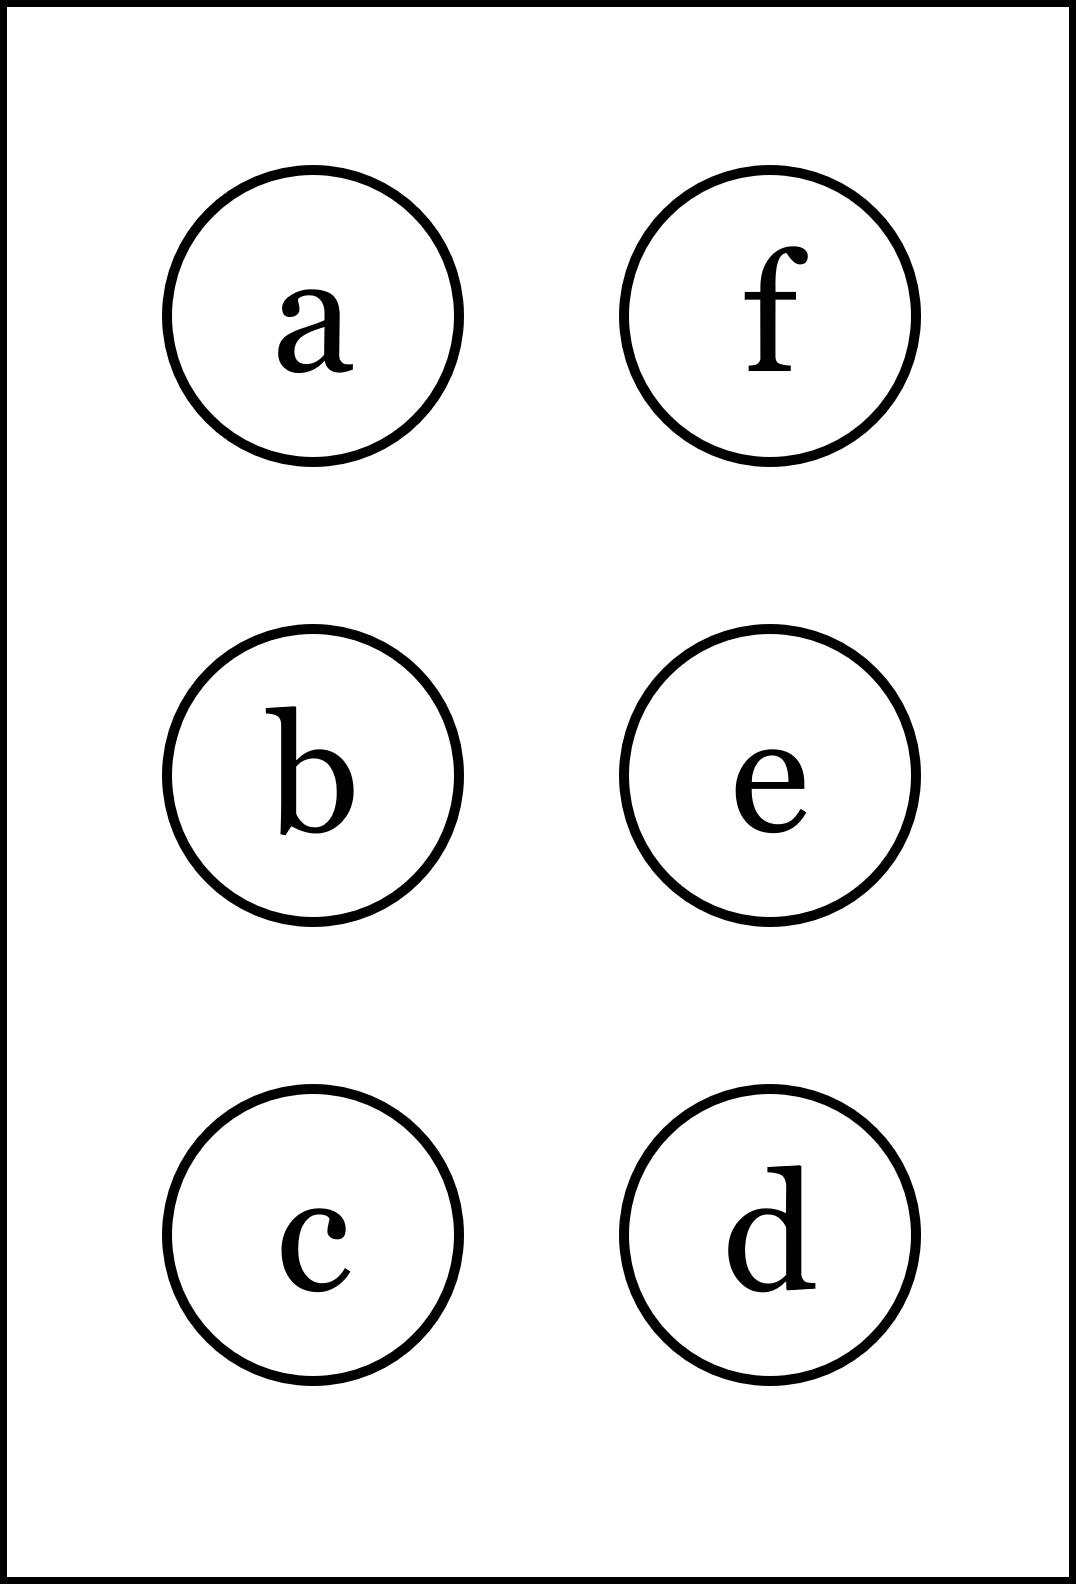
\includegraphics[height=40mm]{../images/braille.png}
{\small Písmeno Braillovej abecedy}
\end{center}
\end{minipage}
\end{center}
\end{minipage}
%
\end{tabular}
\newpage
\thispagestyle{empty}
\begin{tabular}{c:c}
\begin{minipage}[c][104.5mm][t]{0.5\linewidth}
\begin{center}
\vspace{7mm}
{\huge Viazané extrémy, skupina \textit{Mu $\mu$} -\romannumeral1}\\[5mm]
\textit{Jméno:}\phantom{xxxxxxxxxxxxxxxxxxxxxxxxxxxxxxxxxxxxxxxxxxxxxxxxxxxxxxxxxxxxxxxxx}\\[5mm]
\begin{minipage}{0.95\linewidth}
\begin{center}
Cílem je najít \textbf{vázané extrémy} funkce $f(x,y)$ zadané v \textbf{(a)} spolu s vazbou (podmínkou). Postupuj podle krokú v \textbf{(b)} až \textbf{(f)}. Pokud se medzivýsledky shodujú s těmi za otazníky,\\tak napravo obarvi příslušející kroužek načerno. \textbf{Spolu odevzdejte výsledné slovo}.
\end{center}
\end{minipage}
\\[1mm]
\begin{minipage}{0.79\linewidth}
\begin{center}
\begin{varwidth}{\linewidth}
\begin{enumerate}
\normalsize
\item $f(x,y)=-3x+4y-2 \enspace , \enspace \mathrm{vazba:} \enspace x^2+y^2=25$\quad \dotfill\; ???\;\dotfill \quad vybarvi
\item Sestav $L(\lambda,x,y)$ a spočti $\pdv{L}{x}=$\quad \dotfill\; ???\;\dotfill \quad $-3+\lambda x$
\item Takisto spočti $\pdv{L}{y}=$\quad \dotfill\; ???\;\dotfill \quad $4+2\lambda y$
\item Z podmínek $\pdv{L}{x}=0 , \pdv{L}{y}=0$ vyjádři $x,y$ v závislosti na $\lambda$.\\ \phantom{xxxxxx}Následne $x,y$ dosaď do vazbové rovnice\\ \phantom{xxxxxx}a vypočti dva výsledky pro $\lambda$.\quad \dotfill\; ???\;\dotfill \quad $\lambda_1+\lambda_2=-1$
\item Pomocou $\lambda$ urč dvě dvojice pro $x,y$.\quad \dotfill\; ???\;\dotfill \quad $x_1 x_2 y_1 y_2=36$
\item Najdi funkční hodnoty pro oba vázané stacionární body\\ \phantom{xxxxxx}a vyber tu najvětší. $f_{\text{max}}(x,y)=$\quad \dotfill\; ???\;\dotfill \quad $23$
\end{enumerate}
\end{varwidth}
\end{center}
\end{minipage}
\begin{minipage}{0.20\linewidth}
\begin{center}
{\Huge\bfseries 1.} \\[2mm]
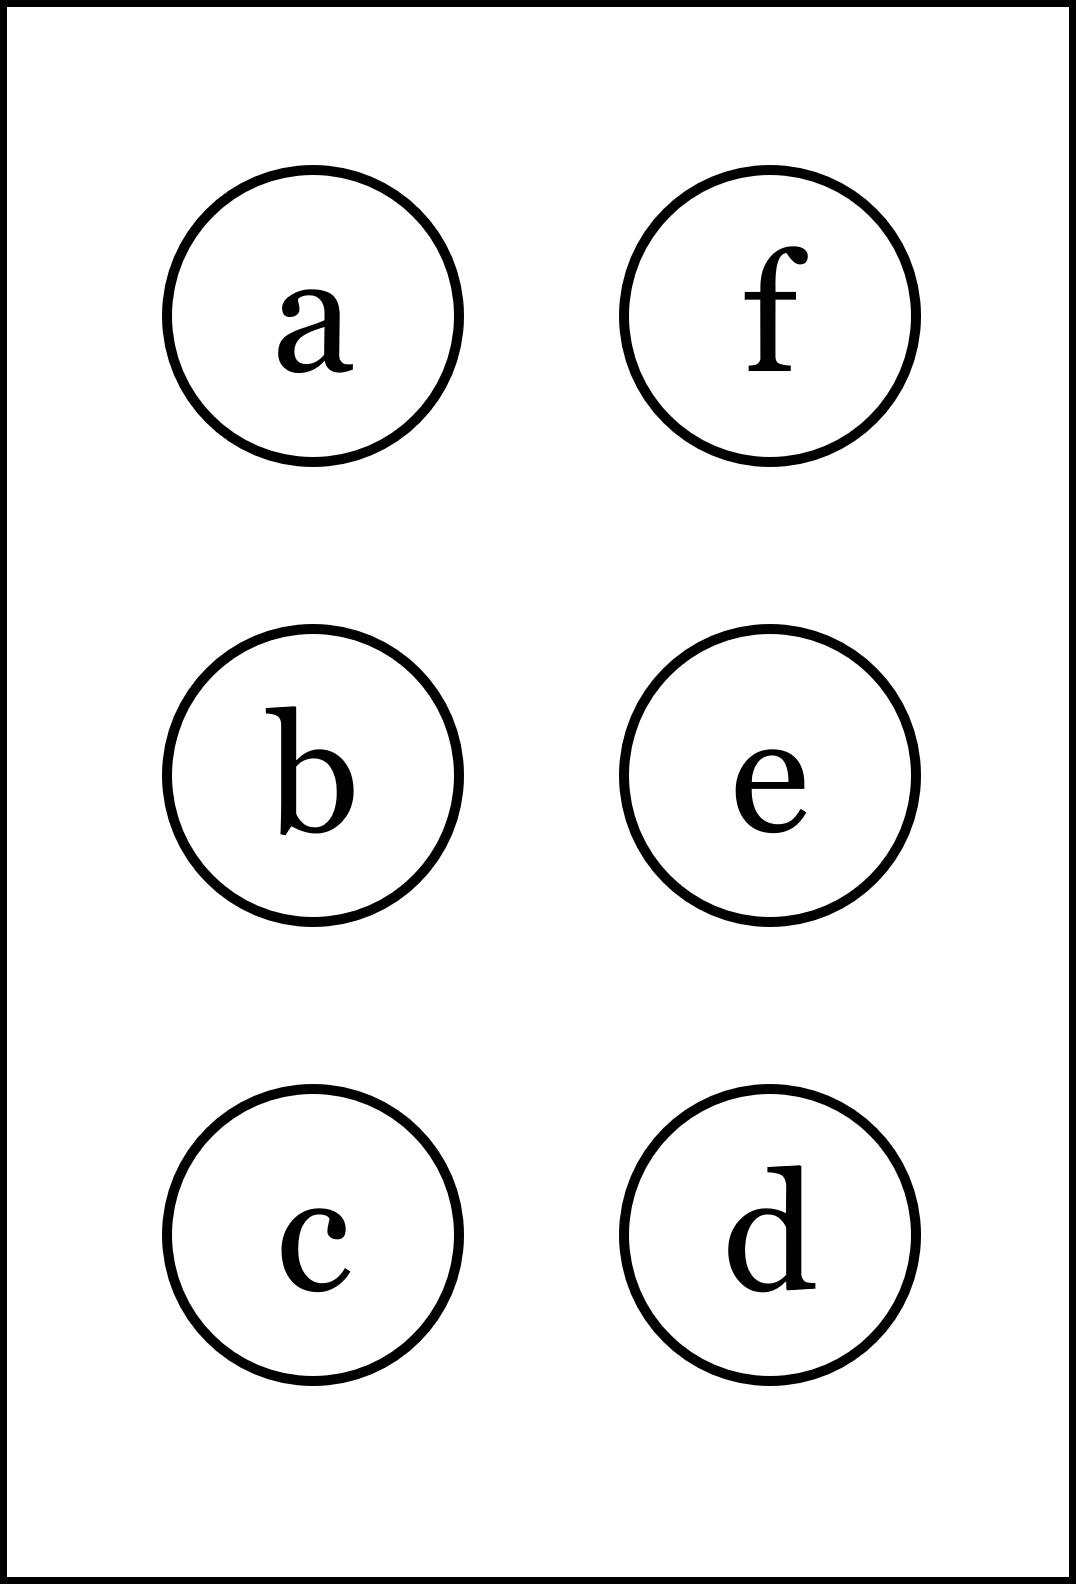
\includegraphics[height=40mm]{../images/braille.png}
{\small Písmeno Braillovej abecedy}
\end{center}
\end{minipage}
\end{center}
\end{minipage}
&
\begin{minipage}[c][104.5mm][t]{0.5\linewidth}
\begin{center}
\vspace{7mm}
{\huge Viazané extrémy, skupina \textit{Mu $\mu$} -\romannumeral2}\\[5mm]
\textit{Jméno:}\phantom{xxxxxxxxxxxxxxxxxxxxxxxxxxxxxxxxxxxxxxxxxxxxxxxxxxxxxxxxxxxxxxxxx}\\[5mm]
\begin{minipage}{0.95\linewidth}
\begin{center}
Cílem je najít \textbf{vázané extrémy} funkce $f(x,y)$ zadané v \textbf{(a)} spolu s vazbou (podmínkou). Postupuj podle krokú v \textbf{(b)} až \textbf{(f)}. Pokud se medzivýsledky shodujú s těmi za otazníky,\\tak napravo obarvi příslušející kroužek načerno. \textbf{Spolu odevzdejte výsledné slovo}.
\end{center}
\end{minipage}
\\[1mm]
\begin{minipage}{0.79\linewidth}
\begin{center}
\begin{varwidth}{\linewidth}
\begin{enumerate}
\normalsize
\item $f(x,y)=-5x+12y-3 \enspace , \enspace \mathrm{vazba:} \enspace x^2+y^2=169$\quad \dotfill\; ???\;\dotfill \quad vybarvi
\item Sestav $L(\lambda,x,y)$ a spočti $\pdv{L}{x}=$\quad \dotfill\; ???\;\dotfill \quad $-5+\lambda x$
\item Takisto spočti $\pdv{L}{y}=$\quad \dotfill\; ???\;\dotfill \quad $12+2\lambda y$
\item Z podmínek $\pdv{L}{x}=0 , \pdv{L}{y}=0$ vyjádři $x,y$ v závislosti na $\lambda$.\\ \phantom{xxxxxx}Následne $x,y$ dosaď do vazbové rovnice\\ \phantom{xxxxxx}a vypočti dva výsledky pro $\lambda$.\quad \dotfill\; ???\;\dotfill \quad $\lambda_1+\lambda_2=-1$
\item Pomocou $\lambda$ urč dvě dvojice pro $x,y$.\quad \dotfill\; ???\;\dotfill \quad $x_1 x_2 y_1 y_2=3600$
\item Najdi funkční hodnoty pro oba vázané stacionární body\\ \phantom{xxxxxx}a vyber tu najvětší. $f_{\text{max}}(x,y)=$\quad \dotfill\; ???\;\dotfill \quad $165$
\end{enumerate}
\end{varwidth}
\end{center}
\end{minipage}
\begin{minipage}{0.20\linewidth}
\begin{center}
{\Huge\bfseries 2.} \\[2mm]
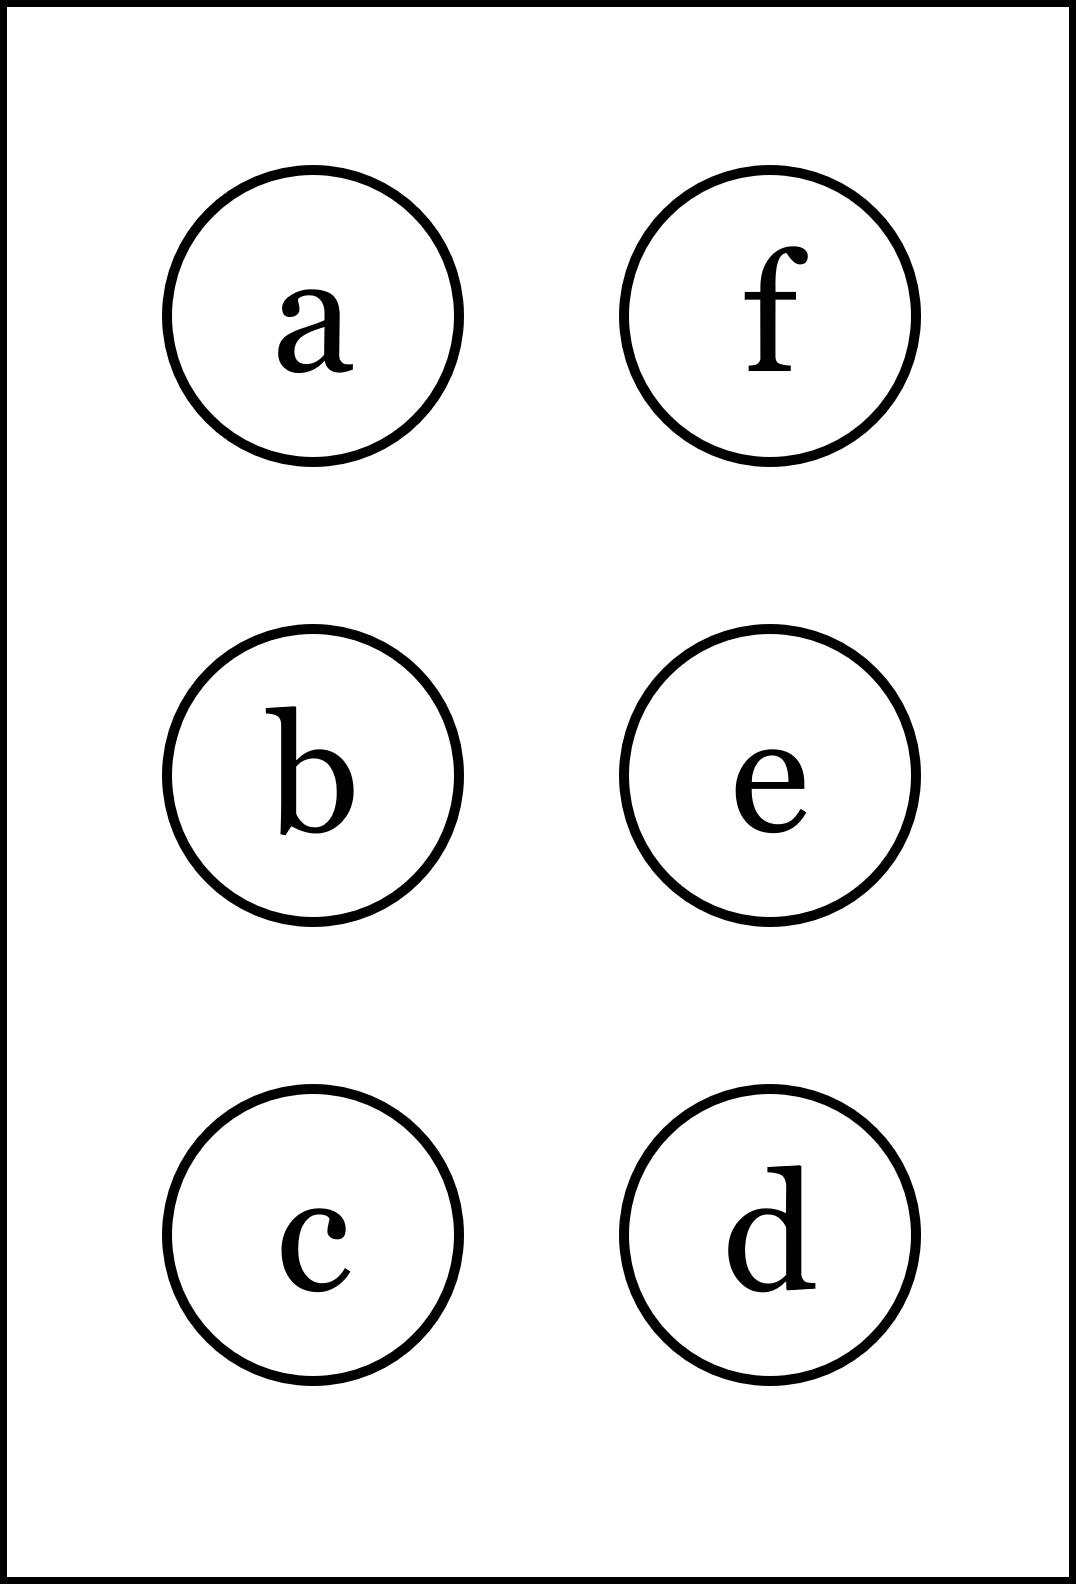
\includegraphics[height=40mm]{../images/braille.png}
{\small Písmeno Braillovej abecedy}
\end{center}
\end{minipage}
\end{center}
\end{minipage}
\\ \hdashline
\begin{minipage}[c][104.5mm][t]{0.5\linewidth}
\begin{center}
\vspace{7mm}
{\huge Viazané extrémy, skupina \textit{Mu $\mu$} -\romannumeral3}\\[5mm]
\textit{Jméno:}\phantom{xxxxxxxxxxxxxxxxxxxxxxxxxxxxxxxxxxxxxxxxxxxxxxxxxxxxxxxxxxxxxxxxx}\\[5mm]
\begin{minipage}{0.95\linewidth}
\begin{center}
Cílem je najít \textbf{vázané extrémy} funkce $f(x,y)$ zadané v \textbf{(a)} spolu s vazbou (podmínkou). Postupuj podle krokú v \textbf{(b)} až \textbf{(f)}. Pokud se medzivýsledky shodujú s těmi za otazníky,\\tak napravo obarvi příslušející kroužek načerno. \textbf{Spolu odevzdejte výsledné slovo}.
\end{center}
\end{minipage}
\\[1mm]
\begin{minipage}{0.79\linewidth}
\begin{center}
\begin{varwidth}{\linewidth}
\begin{enumerate}
\normalsize
\item $f(x,y)=-6x-8y-3 \enspace , \enspace \mathrm{vazba:} \enspace x^2+y^2=100$\quad \dotfill\; ???\;\dotfill \quad nebarvi
\item Sestav $L(\lambda,x,y)$ a spočti $\pdv{L}{x}=$\quad \dotfill\; ???\;\dotfill \quad $-6+2\lambda x$
\item Takisto spočti $\pdv{L}{y}=$\quad \dotfill\; ???\;\dotfill \quad $-8+2\lambda y$
\item Z podmínek $\pdv{L}{x}=0 , \pdv{L}{y}=0$ vyjádři $x,y$ v závislosti na $\lambda$.\\ \phantom{xxxxxx}Následne $x,y$ dosaď do vazbové rovnice\\ \phantom{xxxxxx}a vypočti dva výsledky pro $\lambda$.\quad \dotfill\; ???\;\dotfill \quad $\lambda_1+\lambda_2=1$
\item Pomocou $\lambda$ urč dvě dvojice pro $x,y$.\quad \dotfill\; ???\;\dotfill \quad $x_1 x_2 y_1 y_2=-288$
\item Najdi funkční hodnoty pro oba vázané stacionární body\\ \phantom{xxxxxx}a vyber tu najvětší. $f_{\text{max}}(x,y)=$\quad \dotfill\; ???\;\dotfill \quad $97$
\end{enumerate}
\end{varwidth}
\end{center}
\end{minipage}
\begin{minipage}{0.20\linewidth}
\begin{center}
{\Huge\bfseries 3.} \\[2mm]
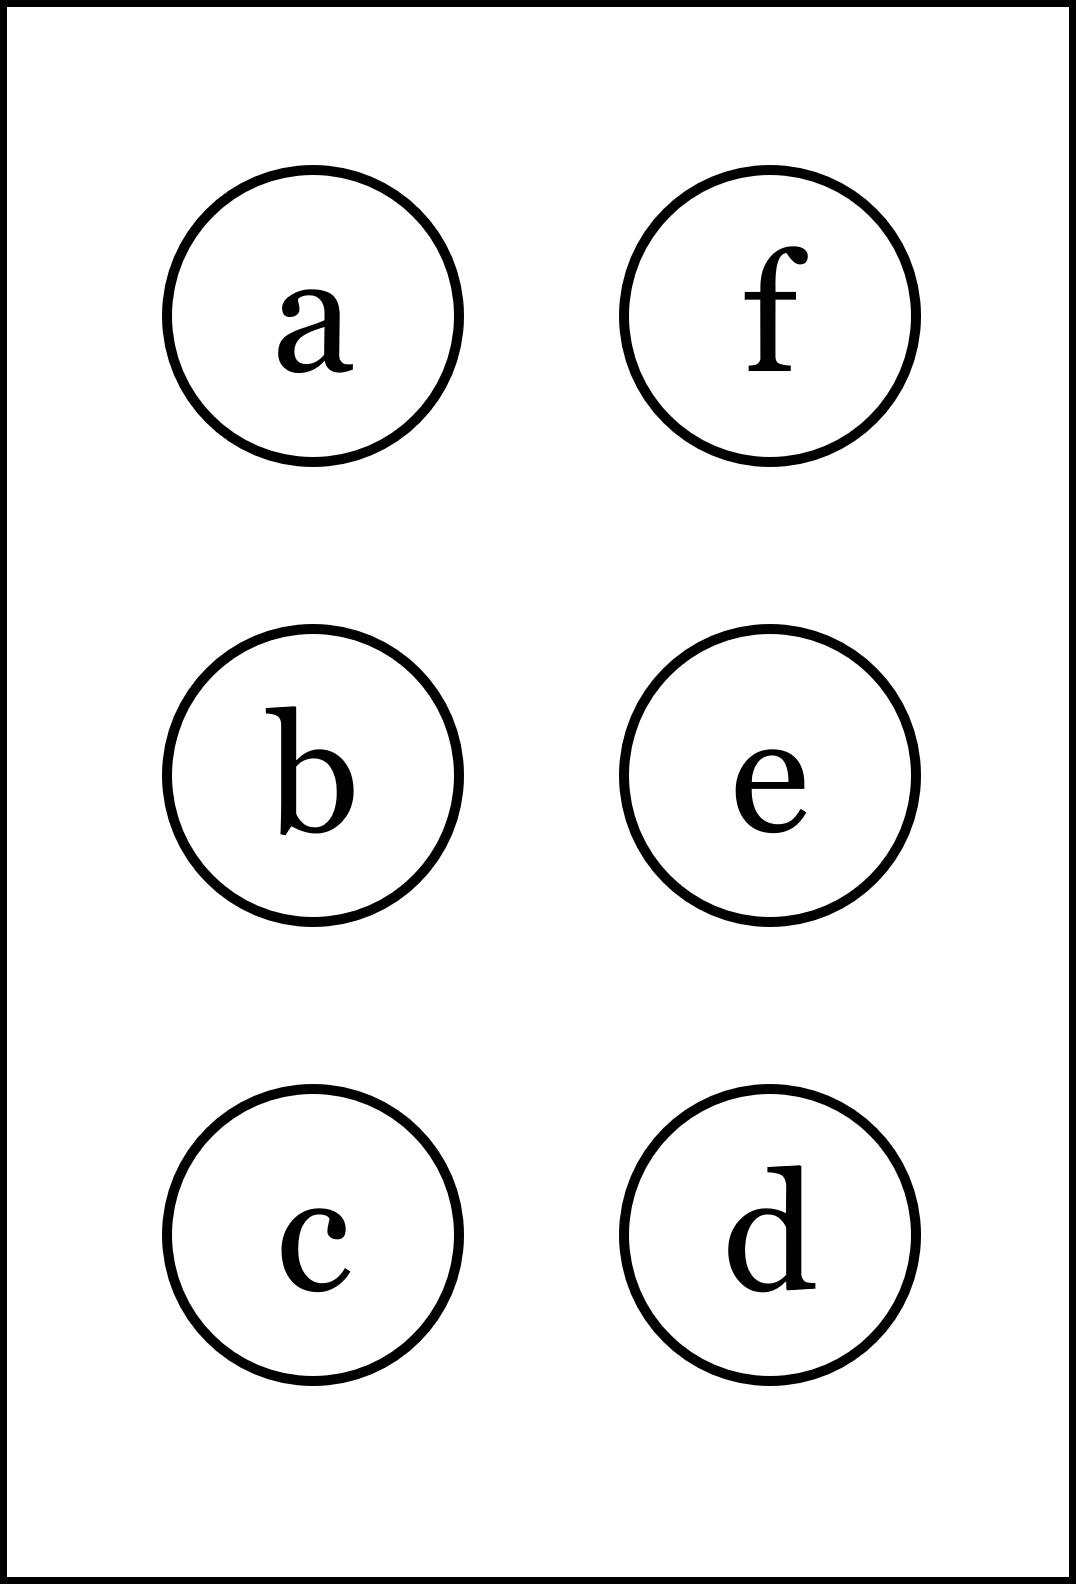
\includegraphics[height=40mm]{../images/braille.png}
{\small Písmeno Braillovej abecedy}
\end{center}
\end{minipage}
\end{center}
\end{minipage}
&
\begin{minipage}[c][104.5mm][t]{0.5\linewidth}
\begin{center}
\vspace{7mm}
{\huge Viazané extrémy, skupina \textit{Mu $\mu$} -\romannumeral4}\\[5mm]
\textit{Jméno:}\phantom{xxxxxxxxxxxxxxxxxxxxxxxxxxxxxxxxxxxxxxxxxxxxxxxxxxxxxxxxxxxxxxxxx}\\[5mm]
\begin{minipage}{0.95\linewidth}
\begin{center}
Cílem je najít \textbf{vázané extrémy} funkce $f(x,y)$ zadané v \textbf{(a)} spolu s vazbou (podmínkou). Postupuj podle krokú v \textbf{(b)} až \textbf{(f)}. Pokud se medzivýsledky shodujú s těmi za otazníky,\\tak napravo obarvi příslušející kroužek načerno. \textbf{Spolu odevzdejte výsledné slovo}.
\end{center}
\end{minipage}
\\[1mm]
\begin{minipage}{0.79\linewidth}
\begin{center}
\begin{varwidth}{\linewidth}
\begin{enumerate}
\normalsize
\item $f(x,y)=10x-24y+4 \enspace , \enspace \mathrm{vazba:} \enspace x^2+y^2=676$\quad \dotfill\; ???\;\dotfill \quad nebarvi
\item Sestav $L(\lambda,x,y)$ a spočti $\pdv{L}{x}=$\quad \dotfill\; ???\;\dotfill \quad $10+2\lambda x$
\item Takisto spočti $\pdv{L}{y}=$\quad \dotfill\; ???\;\dotfill \quad $-24+2\lambda y$
\item Z podmínek $\pdv{L}{x}=0 , \pdv{L}{y}=0$ vyjádři $x,y$ v závislosti na $\lambda$.\\ \phantom{xxxxxx}Následne $x,y$ dosaď do vazbové rovnice\\ \phantom{xxxxxx}a vypočti dva výsledky pro $\lambda$.\quad \dotfill\; ???\;\dotfill \quad $\lambda_1+\lambda_2=-1$
\item Pomocou $\lambda$ urč dvě dvojice pro $x,y$.\quad \dotfill\; ???\;\dotfill \quad $x_1 x_2 y_1 y_2=57600$
\item Najdi funkční hodnoty pro oba vázané stacionární body\\ \phantom{xxxxxx}a vyber tu najvětší. $f_{\text{max}}(x,y)=$\quad \dotfill\; ???\;\dotfill \quad $680$
\end{enumerate}
\end{varwidth}
\end{center}
\end{minipage}
\begin{minipage}{0.20\linewidth}
\begin{center}
{\Huge\bfseries 4.} \\[2mm]
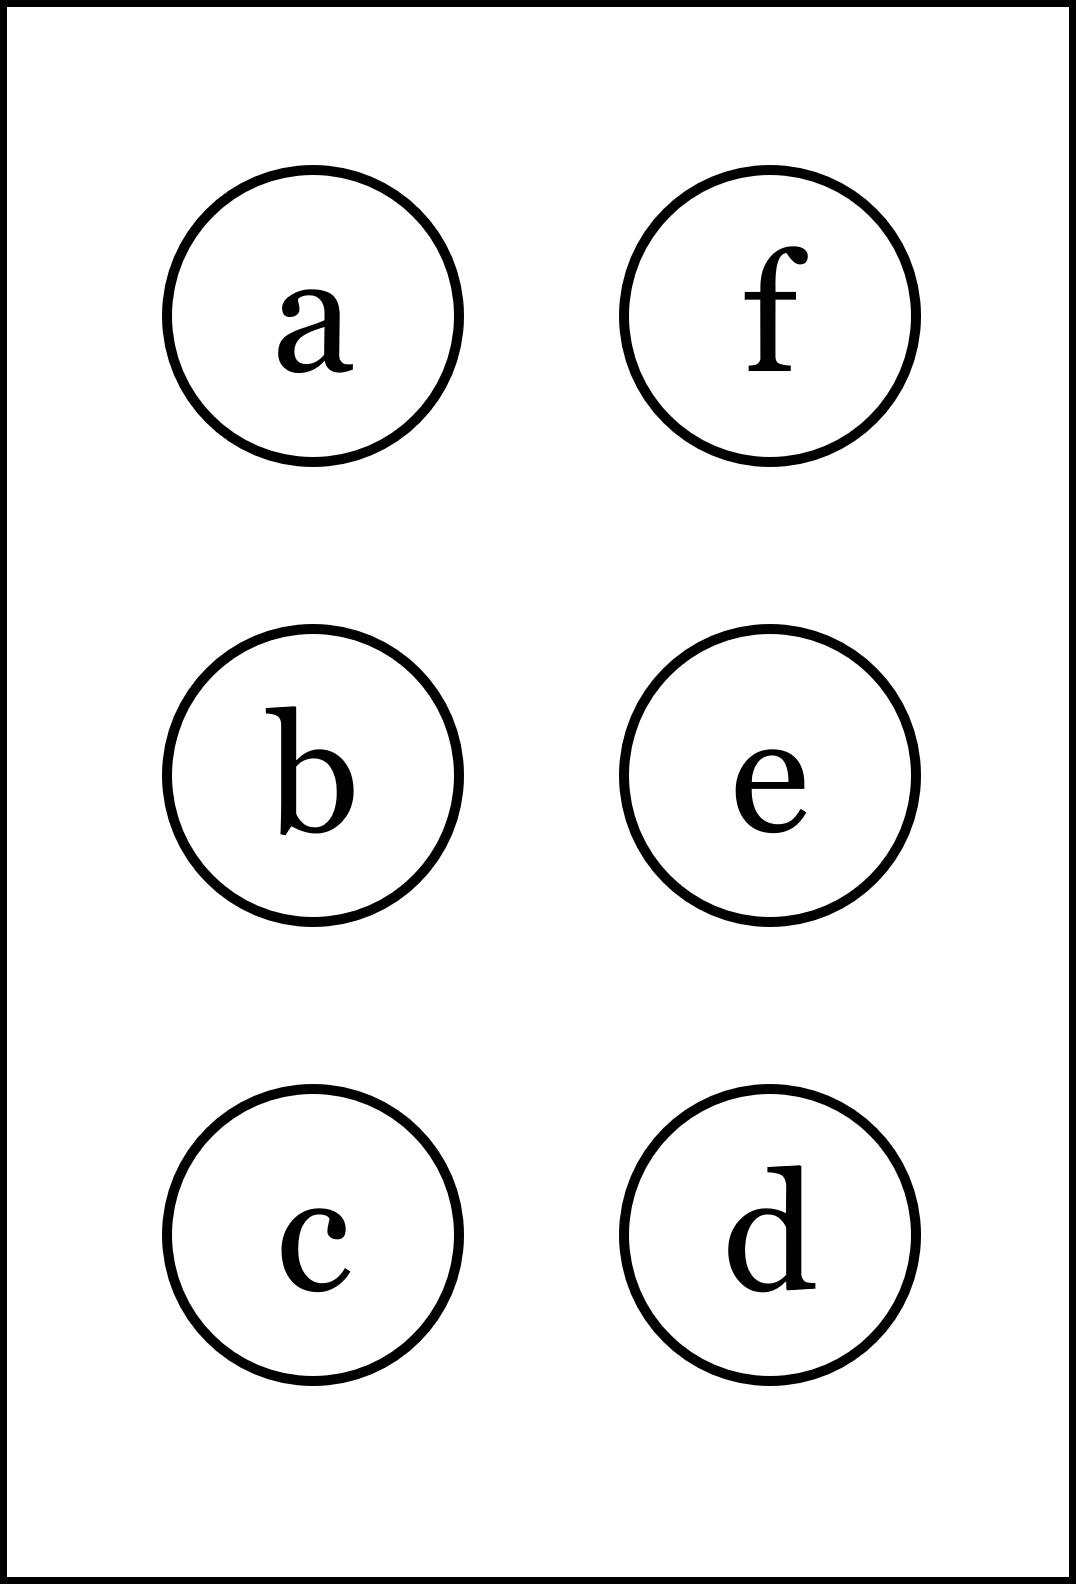
\includegraphics[height=40mm]{../images/braille.png}
{\small Písmeno Braillovej abecedy}
\end{center}
\end{minipage}
\end{center}
\end{minipage}
%
\end{tabular}
\newpage
\thispagestyle{empty}
\begin{tabular}{c:c}
\begin{minipage}[c][104.5mm][t]{0.5\linewidth}
\begin{center}
\vspace{7mm}
{\huge Viazané extrémy, skupina \textit{Nu $\nu$} -\romannumeral1}\\[5mm]
\textit{Jméno:}\phantom{xxxxxxxxxxxxxxxxxxxxxxxxxxxxxxxxxxxxxxxxxxxxxxxxxxxxxxxxxxxxxxxxx}\\[5mm]
\begin{minipage}{0.95\linewidth}
\begin{center}
Cílem je najít \textbf{vázané extrémy} funkce $f(x,y)$ zadané v \textbf{(a)} spolu s vazbou (podmínkou). Postupuj podle krokú v \textbf{(b)} až \textbf{(f)}. Pokud se medzivýsledky shodujú s těmi za otazníky,\\tak napravo obarvi příslušející kroužek načerno. \textbf{Spolu odevzdejte výsledné slovo}.
\end{center}
\end{minipage}
\\[1mm]
\begin{minipage}{0.79\linewidth}
\begin{center}
\begin{varwidth}{\linewidth}
\begin{enumerate}
\normalsize
\item $f(x,y)=3x-4y+1 \enspace , \enspace \mathrm{vazba:} \enspace x^2+y^2=25$\quad \dotfill\; ???\;\dotfill \quad vybarvi
\item Sestav $L(\lambda,x,y)$ a spočti $\pdv{L}{x}=$\quad \dotfill\; ???\;\dotfill \quad $3+2\lambda x$
\item Takisto spočti $\pdv{L}{y}=$\quad \dotfill\; ???\;\dotfill \quad $-4+2\lambda y$
\item Z podmínek $\pdv{L}{x}=0 , \pdv{L}{y}=0$ vyjádři $x,y$ v závislosti na $\lambda$.\\ \phantom{xxxxxx}Následne $x,y$ dosaď do vazbové rovnice\\ \phantom{xxxxxx}a vypočti dva výsledky pro $\lambda$.\quad \dotfill\; ???\;\dotfill \quad $\lambda_1+\lambda_2=1$
\item Pomocou $\lambda$ urč dvě dvojice pro $x,y$.\quad \dotfill\; ???\;\dotfill \quad $x_1 x_2 y_1 y_2=144$
\item Najdi funkční hodnoty pro oba vázané stacionární body\\ \phantom{xxxxxx}a vyber tu najvětší. $f_{\text{max}}(x,y)=$\quad \dotfill\; ???\;\dotfill \quad $25$
\end{enumerate}
\end{varwidth}
\end{center}
\end{minipage}
\begin{minipage}{0.20\linewidth}
\begin{center}
{\Huge\bfseries 1.} \\[2mm]
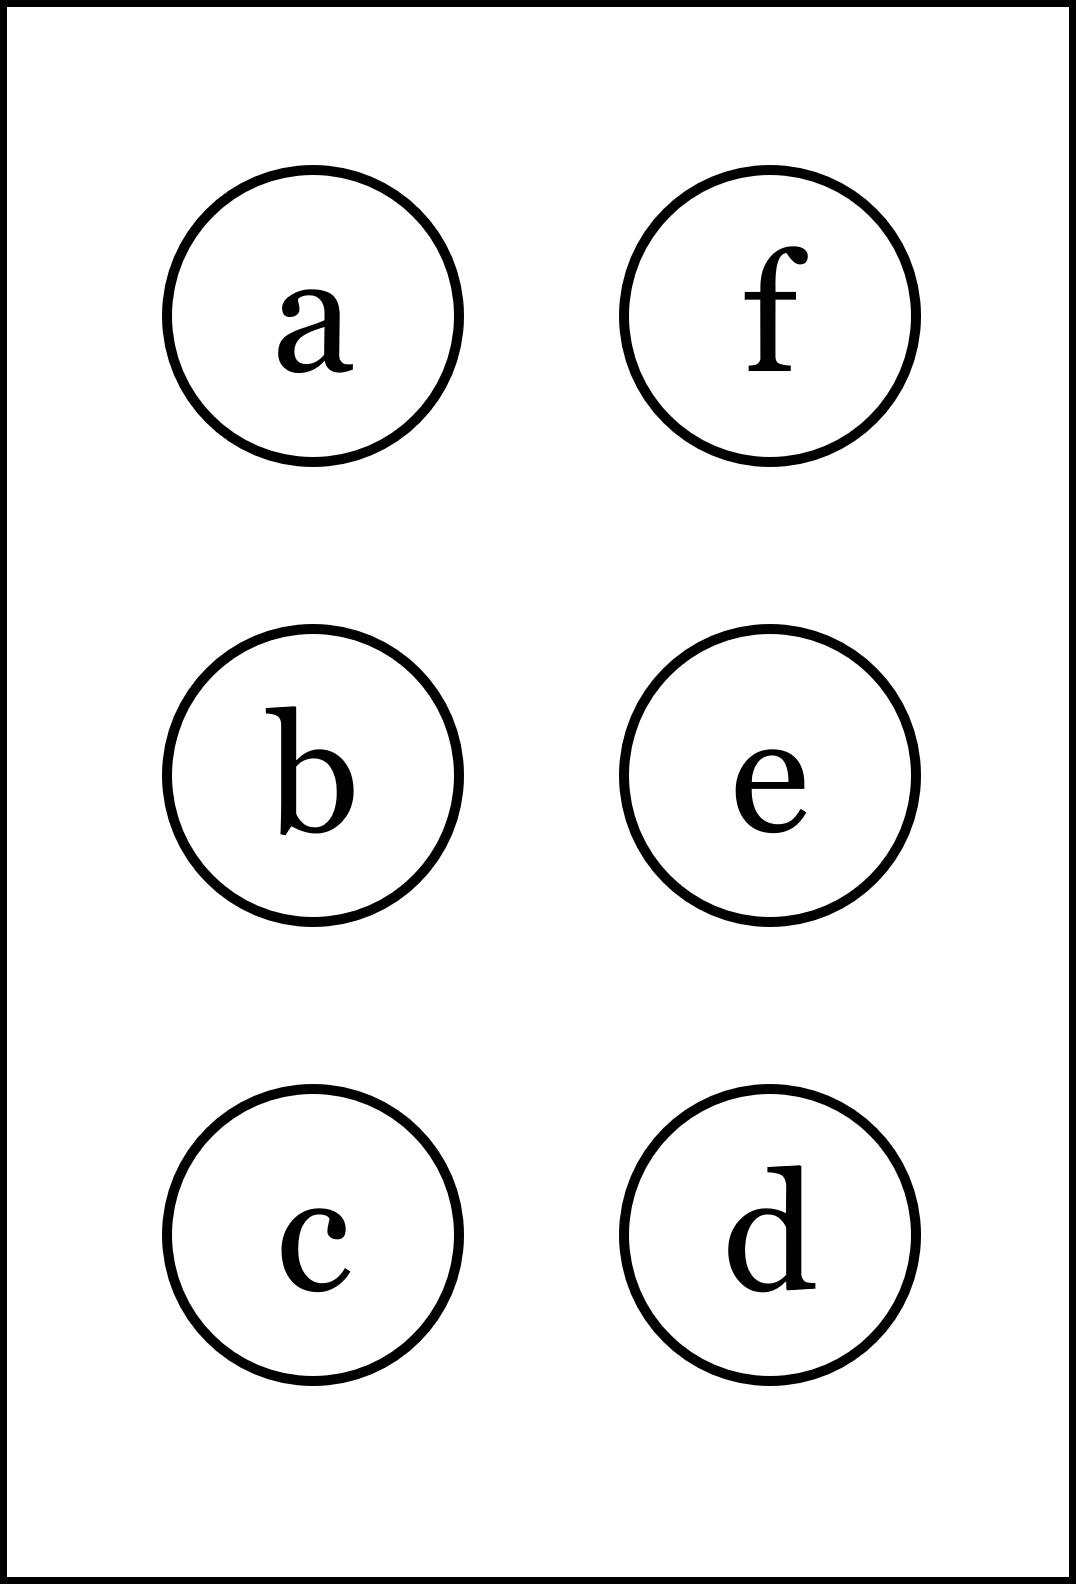
\includegraphics[height=40mm]{../images/braille.png}
{\small Písmeno Braillovej abecedy}
\end{center}
\end{minipage}
\end{center}
\end{minipage}
&
\begin{minipage}[c][104.5mm][t]{0.5\linewidth}
\begin{center}
\vspace{7mm}
{\huge Viazané extrémy, skupina \textit{Nu $\nu$} -\romannumeral2}\\[5mm]
\textit{Jméno:}\phantom{xxxxxxxxxxxxxxxxxxxxxxxxxxxxxxxxxxxxxxxxxxxxxxxxxxxxxxxxxxxxxxxxx}\\[5mm]
\begin{minipage}{0.95\linewidth}
\begin{center}
Cílem je najít \textbf{vázané extrémy} funkce $f(x,y)$ zadané v \textbf{(a)} spolu s vazbou (podmínkou). Postupuj podle krokú v \textbf{(b)} až \textbf{(f)}. Pokud se medzivýsledky shodujú s těmi za otazníky,\\tak napravo obarvi příslušející kroužek načerno. \textbf{Spolu odevzdejte výsledné slovo}.
\end{center}
\end{minipage}
\\[1mm]
\begin{minipage}{0.79\linewidth}
\begin{center}
\begin{varwidth}{\linewidth}
\begin{enumerate}
\normalsize
\item $f(x,y)=5x-12y+1 \enspace , \enspace \mathrm{vazba:} \enspace x^2+y^2=169$\quad \dotfill\; ???\;\dotfill \quad vybarvi
\item Sestav $L(\lambda,x,y)$ a spočti $\pdv{L}{x}=$\quad \dotfill\; ???\;\dotfill \quad $5+\lambda x$
\item Takisto spočti $\pdv{L}{y}=$\quad \dotfill\; ???\;\dotfill \quad $-12+2\lambda y$
\item Z podmínek $\pdv{L}{x}=0 , \pdv{L}{y}=0$ vyjádři $x,y$ v závislosti na $\lambda$.\\ \phantom{xxxxxx}Následne $x,y$ dosaď do vazbové rovnice\\ \phantom{xxxxxx}a vypočti dva výsledky pro $\lambda$.\quad \dotfill\; ???\;\dotfill \quad $\lambda_1+\lambda_2=0$
\item Pomocou $\lambda$ urč dvě dvojice pro $x,y$.\quad \dotfill\; ???\;\dotfill \quad $x_1 x_2 y_1 y_2=3600$
\item Najdi funkční hodnoty pro oba vázané stacionární body\\ \phantom{xxxxxx}a vyber tu najvětší. $f_{\text{max}}(x,y)=$\quad \dotfill\; ???\;\dotfill \quad $170$
\end{enumerate}
\end{varwidth}
\end{center}
\end{minipage}
\begin{minipage}{0.20\linewidth}
\begin{center}
{\Huge\bfseries 2.} \\[2mm]
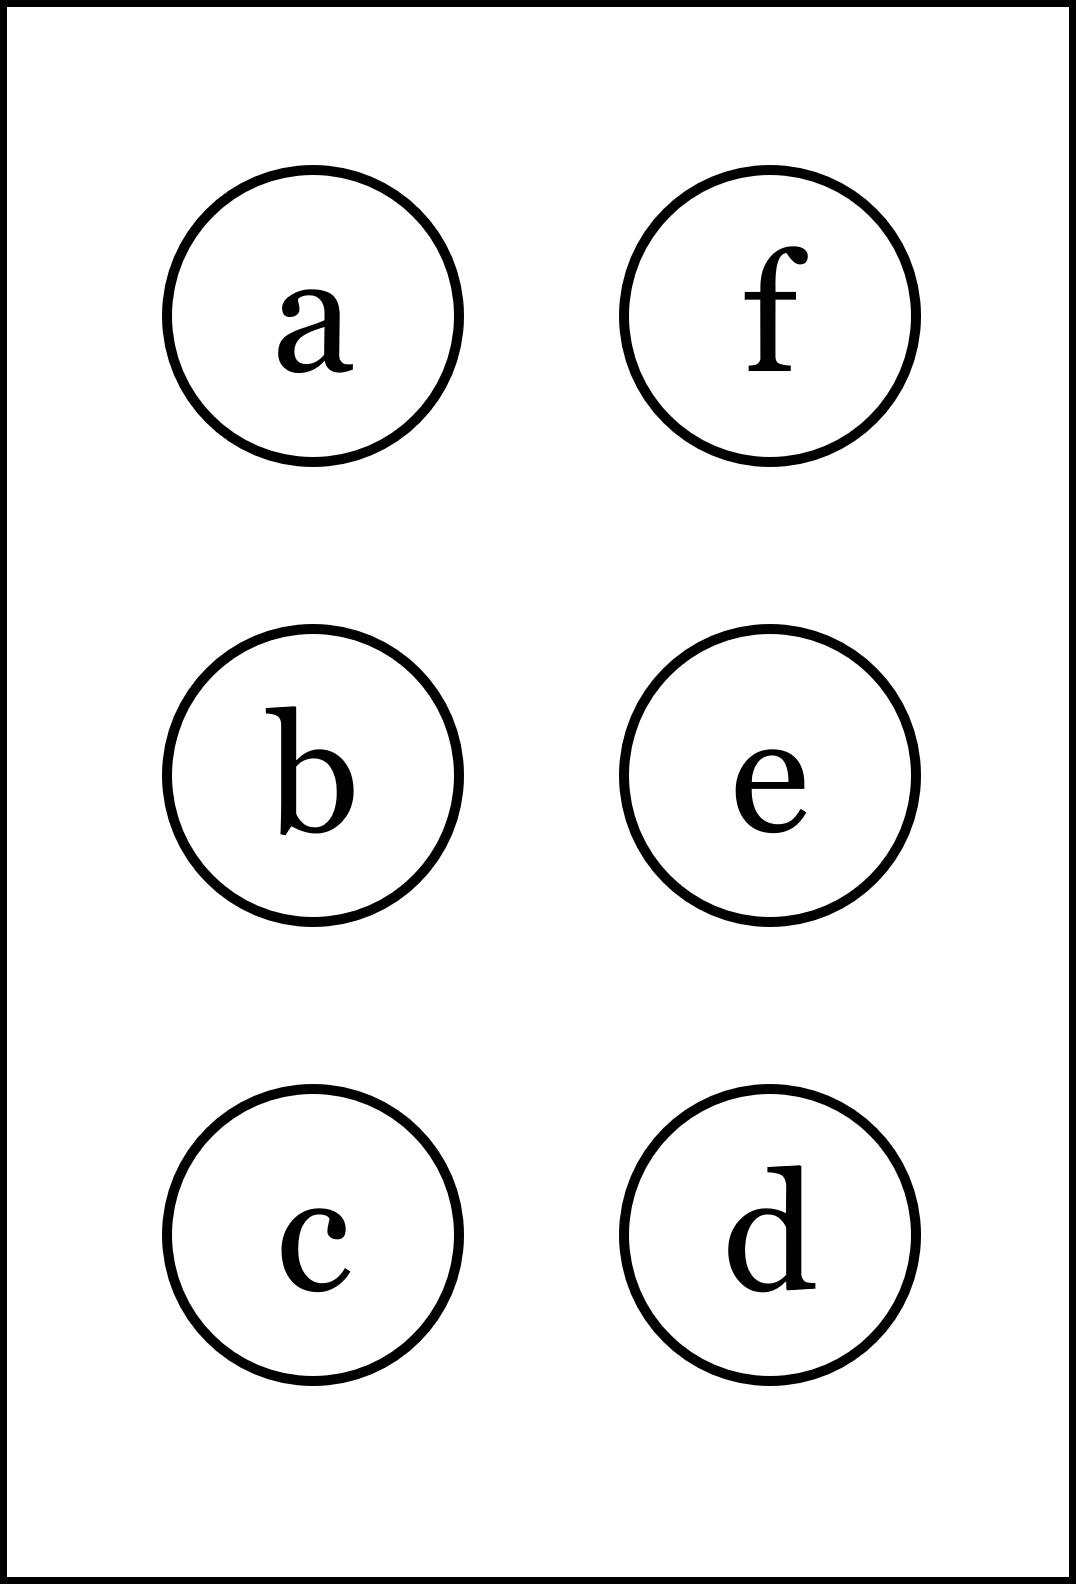
\includegraphics[height=40mm]{../images/braille.png}
{\small Písmeno Braillovej abecedy}
\end{center}
\end{minipage}
\end{center}
\end{minipage}
\\ \hdashline
\begin{minipage}[c][104.5mm][t]{0.5\linewidth}
\begin{center}
\vspace{7mm}
{\huge Viazané extrémy, skupina \textit{Nu $\nu$} -\romannumeral3}\\[5mm]
\textit{Jméno:}\phantom{xxxxxxxxxxxxxxxxxxxxxxxxxxxxxxxxxxxxxxxxxxxxxxxxxxxxxxxxxxxxxxxxx}\\[5mm]
\begin{minipage}{0.95\linewidth}
\begin{center}
Cílem je najít \textbf{vázané extrémy} funkce $f(x,y)$ zadané v \textbf{(a)} spolu s vazbou (podmínkou). Postupuj podle krokú v \textbf{(b)} až \textbf{(f)}. Pokud se medzivýsledky shodujú s těmi za otazníky,\\tak napravo obarvi příslušející kroužek načerno. \textbf{Spolu odevzdejte výsledné slovo}.
\end{center}
\end{minipage}
\\[1mm]
\begin{minipage}{0.79\linewidth}
\begin{center}
\begin{varwidth}{\linewidth}
\begin{enumerate}
\normalsize
\item $f(x,y)=-6x-8y-3 \enspace , \enspace \mathrm{vazba:} \enspace x^2+y^2=100$\quad \dotfill\; ???\;\dotfill \quad vybarvi
\item Sestav $L(\lambda,x,y)$ a spočti $\pdv{L}{x}=$\quad \dotfill\; ???\;\dotfill \quad $-6+2\lambda x$
\item Takisto spočti $\pdv{L}{y}=$\quad \dotfill\; ???\;\dotfill \quad $+8+2\lambda y$
\item Z podmínek $\pdv{L}{x}=0 , \pdv{L}{y}=0$ vyjádři $x,y$ v závislosti na $\lambda$.\\ \phantom{xxxxxx}Následne $x,y$ dosaď do vazbové rovnice\\ \phantom{xxxxxx}a vypočti dva výsledky pro $\lambda$.\quad \dotfill\; ???\;\dotfill \quad $\lambda_1+\lambda_2=-1$
\item Pomocou $\lambda$ urč dvě dvojice pro $x,y$.\quad \dotfill\; ???\;\dotfill \quad $x_1 x_2 y_1 y_2=-288$
\item Najdi funkční hodnoty pro oba vázané stacionární body\\ \phantom{xxxxxx}a vyber tu najvětší. $f_{\text{max}}(x,y)=$\quad \dotfill\; ???\;\dotfill \quad $96$
\end{enumerate}
\end{varwidth}
\end{center}
\end{minipage}
\begin{minipage}{0.20\linewidth}
\begin{center}
{\Huge\bfseries 3.} \\[2mm]
\includegraphics[height=40mm]{../images/braille.png}
{\small Písmeno Braillovej abecedy}
\end{center}
\end{minipage}
\end{center}
\end{minipage}
&
\begin{minipage}[c][104.5mm][t]{0.5\linewidth}
\begin{center}
\vspace{7mm}
{\huge Viazané extrémy, skupina \textit{Nu $\nu$} -\romannumeral4}\\[5mm]
\textit{Jméno:}\phantom{xxxxxxxxxxxxxxxxxxxxxxxxxxxxxxxxxxxxxxxxxxxxxxxxxxxxxxxxxxxxxxxxx}\\[5mm]
\begin{minipage}{0.95\linewidth}
\begin{center}
Cílem je najít \textbf{vázané extrémy} funkce $f(x,y)$ zadané v \textbf{(a)} spolu s vazbou (podmínkou). Postupuj podle krokú v \textbf{(b)} až \textbf{(f)}. Pokud se medzivýsledky shodujú s těmi za otazníky,\\tak napravo obarvi příslušející kroužek načerno. \textbf{Spolu odevzdejte výsledné slovo}.
\end{center}
\end{minipage}
\\[1mm]
\begin{minipage}{0.79\linewidth}
\begin{center}
\begin{varwidth}{\linewidth}
\begin{enumerate}
\normalsize
\item $f(x,y)=-10x+24y-4 \enspace , \enspace \mathrm{vazba:} \enspace x^2+y^2=676$\quad \dotfill\; ???\;\dotfill \quad vybarvi
\item Sestav $L(\lambda,x,y)$ a spočti $\pdv{L}{x}=$\quad \dotfill\; ???\;\dotfill \quad $-10+\lambda x$
\item Takisto spočti $\pdv{L}{y}=$\quad \dotfill\; ???\;\dotfill \quad $-24+2\lambda y$
\item Z podmínek $\pdv{L}{x}=0 , \pdv{L}{y}=0$ vyjádři $x,y$ v závislosti na $\lambda$.\\ \phantom{xxxxxx}Následne $x,y$ dosaď do vazbové rovnice\\ \phantom{xxxxxx}a vypočti dva výsledky pro $\lambda$.\quad \dotfill\; ???\;\dotfill \quad $\lambda_1+\lambda_2=1$
\item Pomocou $\lambda$ urč dvě dvojice pro $x,y$.\quad \dotfill\; ???\;\dotfill \quad $x_1 x_2 y_1 y_2=2400$
\item Najdi funkční hodnoty pro oba vázané stacionární body\\ \phantom{xxxxxx}a vyber tu najvětší. $f_{\text{max}}(x,y)=$\quad \dotfill\; ???\;\dotfill \quad $671$
\end{enumerate}
\end{varwidth}
\end{center}
\end{minipage}
\begin{minipage}{0.20\linewidth}
\begin{center}
{\Huge\bfseries 4.} \\[2mm]
\includegraphics[height=40mm]{../images/braille.png}
{\small Písmeno Braillovej abecedy}
\end{center}
\end{minipage}
\end{center}
\end{minipage}
%
\end{tabular}
\newpage
\thispagestyle{empty}
\begin{tabular}{c:c}
\begin{minipage}[c][104.5mm][t]{0.5\linewidth}
\begin{center}
\vspace{7mm}
{\huge Viazané extrémy, skupina \textit{Xi $\xi$} -\romannumeral1}\\[5mm]
\textit{Jméno:}\phantom{xxxxxxxxxxxxxxxxxxxxxxxxxxxxxxxxxxxxxxxxxxxxxxxxxxxxxxxxxxxxxxxxx}\\[5mm]
\begin{minipage}{0.95\linewidth}
\begin{center}
Cílem je najít \textbf{vázané extrémy} funkce $f(x,y)$ zadané v \textbf{(a)} spolu s vazbou (podmínkou). Postupuj podle krokú v \textbf{(b)} až \textbf{(f)}. Pokud se medzivýsledky shodujú s těmi za otazníky,\\tak napravo obarvi příslušející kroužek načerno. \textbf{Spolu odevzdejte výsledné slovo}.
\end{center}
\end{minipage}
\\[1mm]
\begin{minipage}{0.79\linewidth}
\begin{center}
\begin{varwidth}{\linewidth}
\begin{enumerate}
\normalsize
\item $f(x,y)=3x+4y+4 \enspace , \enspace \mathrm{vazba:} \enspace x^2+y^2=25$\quad \dotfill\; ???\;\dotfill \quad vybarvi
\item Sestav $L(\lambda,x,y)$ a spočti $\pdv{L}{x}=$\quad \dotfill\; ???\;\dotfill \quad $3+2\lambda x$
\item Takisto spočti $\pdv{L}{y}=$\quad \dotfill\; ???\;\dotfill \quad $-4+2\lambda y$
\item Z podmínek $\pdv{L}{x}=0 , \pdv{L}{y}=0$ vyjádři $x,y$ v závislosti na $\lambda$.\\ \phantom{xxxxxx}Následne $x,y$ dosaď do vazbové rovnice\\ \phantom{xxxxxx}a vypočti dva výsledky pro $\lambda$.\quad \dotfill\; ???\;\dotfill \quad $\lambda_1+\lambda_2=2$
\item Pomocou $\lambda$ urč dvě dvojice pro $x,y$.\quad \dotfill\; ???\;\dotfill \quad $x_1 x_2 y_1 y_2=36$
\item Najdi funkční hodnoty pro oba vázané stacionární body\\ \phantom{xxxxxx}a vyber tu najvětší. $f_{\text{max}}(x,y)=$\quad \dotfill\; ???\;\dotfill \quad $29$
\end{enumerate}
\end{varwidth}
\end{center}
\end{minipage}
\begin{minipage}{0.20\linewidth}
\begin{center}
{\Huge\bfseries 1.} \\[2mm]
\includegraphics[height=40mm]{../images/braille.png}
{\small Písmeno Braillovej abecedy}
\end{center}
\end{minipage}
\end{center}
\end{minipage}
&
\begin{minipage}[c][104.5mm][t]{0.5\linewidth}
\begin{center}
\vspace{7mm}
{\huge Viazané extrémy, skupina \textit{Xi $\xi$} -\romannumeral2}\\[5mm]
\textit{Jméno:}\phantom{xxxxxxxxxxxxxxxxxxxxxxxxxxxxxxxxxxxxxxxxxxxxxxxxxxxxxxxxxxxxxxxxx}\\[5mm]
\begin{minipage}{0.95\linewidth}
\begin{center}
Cílem je najít \textbf{vázané extrémy} funkce $f(x,y)$ zadané v \textbf{(a)} spolu s vazbou (podmínkou). Postupuj podle krokú v \textbf{(b)} až \textbf{(f)}. Pokud se medzivýsledky shodujú s těmi za otazníky,\\tak napravo obarvi příslušející kroužek načerno. \textbf{Spolu odevzdejte výsledné slovo}.
\end{center}
\end{minipage}
\\[1mm]
\begin{minipage}{0.79\linewidth}
\begin{center}
\begin{varwidth}{\linewidth}
\begin{enumerate}
\normalsize
\item $f(x,y)=-5x-12y-1 \enspace , \enspace \mathrm{vazba:} \enspace x^2+y^2=169$\quad \dotfill\; ???\;\dotfill \quad vybarvi
\item Sestav $L(\lambda,x,y)$ a spočti $\pdv{L}{x}=$\quad \dotfill\; ???\;\dotfill \quad $-5+\lambda x$
\item Takisto spočti $\pdv{L}{y}=$\quad \dotfill\; ???\;\dotfill \quad $+12+2\lambda y$
\item Z podmínek $\pdv{L}{x}=0 , \pdv{L}{y}=0$ vyjádři $x,y$ v závislosti na $\lambda$.\\ \phantom{xxxxxx}Následne $x,y$ dosaď do vazbové rovnice\\ \phantom{xxxxxx}a vypočti dva výsledky pro $\lambda$.\quad \dotfill\; ???\;\dotfill \quad $\lambda_1+\lambda_2=-2$
\item Pomocou $\lambda$ urč dvě dvojice pro $x,y$.\quad \dotfill\; ???\;\dotfill \quad $x_1 x_2 y_1 y_2=3600$
\item Najdi funkční hodnoty pro oba vázané stacionární body\\ \phantom{xxxxxx}a vyber tu najvětší. $f_{\text{max}}(x,y)=$\quad \dotfill\; ???\;\dotfill \quad $167$
\end{enumerate}
\end{varwidth}
\end{center}
\end{minipage}
\begin{minipage}{0.20\linewidth}
\begin{center}
{\Huge\bfseries 2.} \\[2mm]
\includegraphics[height=40mm]{../images/braille.png}
{\small Písmeno Braillovej abecedy}
\end{center}
\end{minipage}
\end{center}
\end{minipage}
\\ \hdashline
\begin{minipage}[c][104.5mm][t]{0.5\linewidth}
\begin{center}
\vspace{7mm}
{\huge Viazané extrémy, skupina \textit{Xi $\xi$} -\romannumeral3}\\[5mm]
\textit{Jméno:}\phantom{xxxxxxxxxxxxxxxxxxxxxxxxxxxxxxxxxxxxxxxxxxxxxxxxxxxxxxxxxxxxxxxxx}\\[5mm]
\begin{minipage}{0.95\linewidth}
\begin{center}
Cílem je najít \textbf{vázané extrémy} funkce $f(x,y)$ zadané v \textbf{(a)} spolu s vazbou (podmínkou). Postupuj podle krokú v \textbf{(b)} až \textbf{(f)}. Pokud se medzivýsledky shodujú s těmi za otazníky,\\tak napravo obarvi příslušející kroužek načerno. \textbf{Spolu odevzdejte výsledné slovo}.
\end{center}
\end{minipage}
\\[1mm]
\begin{minipage}{0.79\linewidth}
\begin{center}
\begin{varwidth}{\linewidth}
\begin{enumerate}
\normalsize
\item $f(x,y)=-6x-8y+1 \enspace , \enspace \mathrm{vazba:} \enspace x^2+y^2=100$\quad \dotfill\; ???\;\dotfill \quad vybarvi
\item Sestav $L(\lambda,x,y)$ a spočti $\pdv{L}{x}=$\quad \dotfill\; ???\;\dotfill \quad $-6+\lambda x$
\item Takisto spočti $\pdv{L}{y}=$\quad \dotfill\; ???\;\dotfill \quad $-8+2\lambda y$
\item Z podmínek $\pdv{L}{x}=0 , \pdv{L}{y}=0$ vyjádři $x,y$ v závislosti na $\lambda$.\\ \phantom{xxxxxx}Následne $x,y$ dosaď do vazbové rovnice\\ \phantom{xxxxxx}a vypočti dva výsledky pro $\lambda$.\quad \dotfill\; ???\;\dotfill \quad $\lambda_1+\lambda_2=-1$
\item Pomocou $\lambda$ urč dvě dvojice pro $x,y$.\quad \dotfill\; ???\;\dotfill \quad $x_1 x_2 y_1 y_2=2304$
\item Najdi funkční hodnoty pro oba vázané stacionární body\\ \phantom{xxxxxx}a vyber tu najvětší. $f_{\text{max}}(x,y)=$\quad \dotfill\; ???\;\dotfill \quad $101$
\end{enumerate}
\end{varwidth}
\end{center}
\end{minipage}
\begin{minipage}{0.20\linewidth}
\begin{center}
{\Huge\bfseries 3.} \\[2mm]
\includegraphics[height=40mm]{../images/braille.png}
{\small Písmeno Braillovej abecedy}
\end{center}
\end{minipage}
\end{center}
\end{minipage}
&
\begin{minipage}[c][104.5mm][t]{0.5\linewidth}
\begin{center}
\vspace{7mm}
{\huge Viazané extrémy, skupina \textit{Xi $\xi$} -\romannumeral4}\\[5mm]
\textit{Jméno:}\phantom{xxxxxxxxxxxxxxxxxxxxxxxxxxxxxxxxxxxxxxxxxxxxxxxxxxxxxxxxxxxxxxxxx}\\[5mm]
\begin{minipage}{0.95\linewidth}
\begin{center}
Cílem je najít \textbf{vázané extrémy} funkce $f(x,y)$ zadané v \textbf{(a)} spolu s vazbou (podmínkou). Postupuj podle krokú v \textbf{(b)} až \textbf{(f)}. Pokud se medzivýsledky shodujú s těmi za otazníky,\\tak napravo obarvi příslušející kroužek načerno. \textbf{Spolu odevzdejte výsledné slovo}.
\end{center}
\end{minipage}
\\[1mm]
\begin{minipage}{0.79\linewidth}
\begin{center}
\begin{varwidth}{\linewidth}
\begin{enumerate}
\normalsize
\item $f(x,y)=10x-24y+3 \enspace , \enspace \mathrm{vazba:} \enspace x^2+y^2=676$\quad \dotfill\; ???\;\dotfill \quad vybarvi
\item Sestav $L(\lambda,x,y)$ a spočti $\pdv{L}{x}=$\quad \dotfill\; ???\;\dotfill \quad $10+\lambda x$
\item Takisto spočti $\pdv{L}{y}=$\quad \dotfill\; ???\;\dotfill \quad $+24+2\lambda y$
\item Z podmínek $\pdv{L}{x}=0 , \pdv{L}{y}=0$ vyjádři $x,y$ v závislosti na $\lambda$.\\ \phantom{xxxxxx}Následne $x,y$ dosaď do vazbové rovnice\\ \phantom{xxxxxx}a vypočti dva výsledky pro $\lambda$.\quad \dotfill\; ???\;\dotfill \quad $\lambda_1+\lambda_2=-2$
\item Pomocou $\lambda$ urč dvě dvojice pro $x,y$.\quad \dotfill\; ???\;\dotfill \quad $x_1 x_2 y_1 y_2=-2400$
\item Najdi funkční hodnoty pro oba vázané stacionární body\\ \phantom{xxxxxx}a vyber tu najvětší. $f_{\text{max}}(x,y)=$\quad \dotfill\; ???\;\dotfill \quad $678$
\end{enumerate}
\end{varwidth}
\end{center}
\end{minipage}
\begin{minipage}{0.20\linewidth}
\begin{center}
{\Huge\bfseries 4.} \\[2mm]
\includegraphics[height=40mm]{../images/braille.png}
{\small Písmeno Braillovej abecedy}
\end{center}
\end{minipage}
\end{center}
\end{minipage}
%
\end{tabular}
\newpage
\thispagestyle{empty}
\begin{tabular}{c:c}
\begin{minipage}[c][104.5mm][t]{0.5\linewidth}
\begin{center}
\vspace{7mm}
{\huge Viazané extrémy, skupina \textit{Omicron $\omicron$} -\romannumeral1}\\[5mm]
\textit{Jméno:}\phantom{xxxxxxxxxxxxxxxxxxxxxxxxxxxxxxxxxxxxxxxxxxxxxxxxxxxxxxxxxxxxxxxxx}\\[5mm]
\begin{minipage}{0.95\linewidth}
\begin{center}
Cílem je najít \textbf{vázané extrémy} funkce $f(x,y)$ zadané v \textbf{(a)} spolu s vazbou (podmínkou). Postupuj podle krokú v \textbf{(b)} až \textbf{(f)}. Pokud se medzivýsledky shodujú s těmi za otazníky,\\tak napravo obarvi příslušející kroužek načerno. \textbf{Spolu odevzdejte výsledné slovo}.
\end{center}
\end{minipage}
\\[1mm]
\begin{minipage}{0.79\linewidth}
\begin{center}
\begin{varwidth}{\linewidth}
\begin{enumerate}
\normalsize
\item $f(x,y)=3x+4y-3 \enspace , \enspace \mathrm{vazba:} \enspace x^2+y^2=25$\quad \dotfill\; ???\;\dotfill \quad vybarvi
\item Sestav $L(\lambda,x,y)$ a spočti $\pdv{L}{x}=$\quad \dotfill\; ???\;\dotfill \quad $3+\lambda x$
\item Takisto spočti $\pdv{L}{y}=$\quad \dotfill\; ???\;\dotfill \quad $-4+2\lambda y$
\item Z podmínek $\pdv{L}{x}=0 , \pdv{L}{y}=0$ vyjádři $x,y$ v závislosti na $\lambda$.\\ \phantom{xxxxxx}Následne $x,y$ dosaď do vazbové rovnice\\ \phantom{xxxxxx}a vypočti dva výsledky pro $\lambda$.\quad \dotfill\; ???\;\dotfill \quad $\lambda_1+\lambda_2=-2$
\item Pomocou $\lambda$ urč dvě dvojice pro $x,y$.\quad \dotfill\; ???\;\dotfill \quad $x_1 x_2 y_1 y_2=36$
\item Najdi funkční hodnoty pro oba vázané stacionární body\\ \phantom{xxxxxx}a vyber tu najvětší. $f_{\text{max}}(x,y)=$\quad \dotfill\; ???\;\dotfill \quad $22$
\end{enumerate}
\end{varwidth}
\end{center}
\end{minipage}
\begin{minipage}{0.20\linewidth}
\begin{center}
{\Huge\bfseries 1.} \\[2mm]
\includegraphics[height=40mm]{../images/braille.png}
{\small Písmeno Braillovej abecedy}
\end{center}
\end{minipage}
\end{center}
\end{minipage}
&
\begin{minipage}[c][104.5mm][t]{0.5\linewidth}
\begin{center}
\vspace{7mm}
{\huge Viazané extrémy, skupina \textit{Omicron $\omicron$} -\romannumeral2}\\[5mm]
\textit{Jméno:}\phantom{xxxxxxxxxxxxxxxxxxxxxxxxxxxxxxxxxxxxxxxxxxxxxxxxxxxxxxxxxxxxxxxxx}\\[5mm]
\begin{minipage}{0.95\linewidth}
\begin{center}
Cílem je najít \textbf{vázané extrémy} funkce $f(x,y)$ zadané v \textbf{(a)} spolu s vazbou (podmínkou). Postupuj podle krokú v \textbf{(b)} až \textbf{(f)}. Pokud se medzivýsledky shodujú s těmi za otazníky,\\tak napravo obarvi příslušející kroužek načerno. \textbf{Spolu odevzdejte výsledné slovo}.
\end{center}
\end{minipage}
\\[1mm]
\begin{minipage}{0.79\linewidth}
\begin{center}
\begin{varwidth}{\linewidth}
\begin{enumerate}
\normalsize
\item $f(x,y)=-5x-12y-3 \enspace , \enspace \mathrm{vazba:} \enspace x^2+y^2=169$\quad \dotfill\; ???\;\dotfill \quad vybarvi
\item Sestav $L(\lambda,x,y)$ a spočti $\pdv{L}{x}=$\quad \dotfill\; ???\;\dotfill \quad $-5+\lambda x$
\item Takisto spočti $\pdv{L}{y}=$\quad \dotfill\; ???\;\dotfill \quad $-12+2\lambda y$
\item Z podmínek $\pdv{L}{x}=0 , \pdv{L}{y}=0$ vyjádři $x,y$ v závislosti na $\lambda$.\\ \phantom{xxxxxx}Následne $x,y$ dosaď do vazbové rovnice\\ \phantom{xxxxxx}a vypočti dva výsledky pro $\lambda$.\quad \dotfill\; ???\;\dotfill \quad $\lambda_1+\lambda_2=0$
\item Pomocou $\lambda$ urč dvě dvojice pro $x,y$.\quad \dotfill\; ???\;\dotfill \quad $x_1 x_2 y_1 y_2=-300$
\item Najdi funkční hodnoty pro oba vázané stacionární body\\ \phantom{xxxxxx}a vyber tu najvětší. $f_{\text{max}}(x,y)=$\quad \dotfill\; ???\;\dotfill \quad $165$
\end{enumerate}
\end{varwidth}
\end{center}
\end{minipage}
\begin{minipage}{0.20\linewidth}
\begin{center}
{\Huge\bfseries 2.} \\[2mm]
\includegraphics[height=40mm]{../images/braille.png}
{\small Písmeno Braillovej abecedy}
\end{center}
\end{minipage}
\end{center}
\end{minipage}
\\ \hdashline
\begin{minipage}[c][104.5mm][t]{0.5\linewidth}
\begin{center}
\vspace{7mm}
{\huge Viazané extrémy, skupina \textit{Omicron $\omicron$} -\romannumeral3}\\[5mm]
\textit{Jméno:}\phantom{xxxxxxxxxxxxxxxxxxxxxxxxxxxxxxxxxxxxxxxxxxxxxxxxxxxxxxxxxxxxxxxxx}\\[5mm]
\begin{minipage}{0.95\linewidth}
\begin{center}
Cílem je najít \textbf{vázané extrémy} funkce $f(x,y)$ zadané v \textbf{(a)} spolu s vazbou (podmínkou). Postupuj podle krokú v \textbf{(b)} až \textbf{(f)}. Pokud se medzivýsledky shodujú s těmi za otazníky,\\tak napravo obarvi příslušející kroužek načerno. \textbf{Spolu odevzdejte výsledné slovo}.
\end{center}
\end{minipage}
\\[1mm]
\begin{minipage}{0.79\linewidth}
\begin{center}
\begin{varwidth}{\linewidth}
\begin{enumerate}
\normalsize
\item $f(x,y)=-6x-8y+4 \enspace , \enspace \mathrm{vazba:} \enspace x^2+y^2=100$\quad \dotfill\; ???\;\dotfill \quad vybarvi
\item Sestav $L(\lambda,x,y)$ a spočti $\pdv{L}{x}=$\quad \dotfill\; ???\;\dotfill \quad $-6+\lambda x$
\item Takisto spočti $\pdv{L}{y}=$\quad \dotfill\; ???\;\dotfill \quad $-8+2\lambda y$
\item Z podmínek $\pdv{L}{x}=0 , \pdv{L}{y}=0$ vyjádři $x,y$ v závislosti na $\lambda$.\\ \phantom{xxxxxx}Následne $x,y$ dosaď do vazbové rovnice\\ \phantom{xxxxxx}a vypočti dva výsledky pro $\lambda$.\quad \dotfill\; ???\;\dotfill \quad $\lambda_1+\lambda_2=-2$
\item Pomocou $\lambda$ urč dvě dvojice pro $x,y$.\quad \dotfill\; ???\;\dotfill \quad $x_1 x_2 y_1 y_2=-288$
\item Najdi funkční hodnoty pro oba vázané stacionární body\\ \phantom{xxxxxx}a vyber tu najvětší. $f_{\text{max}}(x,y)=$\quad \dotfill\; ???\;\dotfill \quad $103$
\end{enumerate}
\end{varwidth}
\end{center}
\end{minipage}
\begin{minipage}{0.20\linewidth}
\begin{center}
{\Huge\bfseries 3.} \\[2mm]
\includegraphics[height=40mm]{../images/braille.png}
{\small Písmeno Braillovej abecedy}
\end{center}
\end{minipage}
\end{center}
\end{minipage}
&
\begin{minipage}[c][104.5mm][t]{0.5\linewidth}
\begin{center}
\vspace{7mm}
{\huge Viazané extrémy, skupina \textit{Omicron $\omicron$} -\romannumeral4}\\[5mm]
\textit{Jméno:}\phantom{xxxxxxxxxxxxxxxxxxxxxxxxxxxxxxxxxxxxxxxxxxxxxxxxxxxxxxxxxxxxxxxxx}\\[5mm]
\begin{minipage}{0.95\linewidth}
\begin{center}
Cílem je najít \textbf{vázané extrémy} funkce $f(x,y)$ zadané v \textbf{(a)} spolu s vazbou (podmínkou). Postupuj podle krokú v \textbf{(b)} až \textbf{(f)}. Pokud se medzivýsledky shodujú s těmi za otazníky,\\tak napravo obarvi příslušející kroužek načerno. \textbf{Spolu odevzdejte výsledné slovo}.
\end{center}
\end{minipage}
\\[1mm]
\begin{minipage}{0.79\linewidth}
\begin{center}
\begin{varwidth}{\linewidth}
\begin{enumerate}
\normalsize
\item $f(x,y)=-10x+24y-2 \enspace , \enspace \mathrm{vazba:} \enspace x^2+y^2=676$\quad \dotfill\; ???\;\dotfill \quad vybarvi
\item Sestav $L(\lambda,x,y)$ a spočti $\pdv{L}{x}=$\quad \dotfill\; ???\;\dotfill \quad $-10+2\lambda x$
\item Takisto spočti $\pdv{L}{y}=$\quad \dotfill\; ???\;\dotfill \quad $24+2\lambda y$
\item Z podmínek $\pdv{L}{x}=0 , \pdv{L}{y}=0$ vyjádři $x,y$ v závislosti na $\lambda$.\\ \phantom{xxxxxx}Následne $x,y$ dosaď do vazbové rovnice\\ \phantom{xxxxxx}a vypočti dva výsledky pro $\lambda$.\quad \dotfill\; ???\;\dotfill \quad $\lambda_1+\lambda_2=1$
\item Pomocou $\lambda$ urč dvě dvojice pro $x,y$.\quad \dotfill\; ???\;\dotfill \quad $x_1 x_2 y_1 y_2=57600$
\item Najdi funkční hodnoty pro oba vázané stacionární body\\ \phantom{xxxxxx}a vyber tu najvětší. $f_{\text{max}}(x,y)=$\quad \dotfill\; ???\;\dotfill \quad $673$
\end{enumerate}
\end{varwidth}
\end{center}
\end{minipage}
\begin{minipage}{0.20\linewidth}
\begin{center}
{\Huge\bfseries 4.} \\[2mm]
\includegraphics[height=40mm]{../images/braille.png}
{\small Písmeno Braillovej abecedy}
\end{center}
\end{minipage}
\end{center}
\end{minipage}
%
\end{tabular}
\newpage
\thispagestyle{empty}
\begin{tabular}{c:c}
\begin{minipage}[c][104.5mm][t]{0.5\linewidth}
\begin{center}
\vspace{7mm}
{\huge Viazané extrémy, skupina \textit{Pi $\pi$} -\romannumeral1}\\[5mm]
\textit{Jméno:}\phantom{xxxxxxxxxxxxxxxxxxxxxxxxxxxxxxxxxxxxxxxxxxxxxxxxxxxxxxxxxxxxxxxxx}\\[5mm]
\begin{minipage}{0.95\linewidth}
\begin{center}
Cílem je najít \textbf{vázané extrémy} funkce $f(x,y)$ zadané v \textbf{(a)} spolu s vazbou (podmínkou). Postupuj podle krokú v \textbf{(b)} až \textbf{(f)}. Pokud se medzivýsledky shodujú s těmi za otazníky,\\tak napravo obarvi příslušející kroužek načerno. \textbf{Spolu odevzdejte výsledné slovo}.
\end{center}
\end{minipage}
\\[1mm]
\begin{minipage}{0.79\linewidth}
\begin{center}
\begin{varwidth}{\linewidth}
\begin{enumerate}
\normalsize
\item $f(x,y)=-3x+4y-3 \enspace , \enspace \mathrm{vazba:} \enspace x^2+y^2=25$\quad \dotfill\; ???\;\dotfill \quad vybarvi
\item Sestav $L(\lambda,x,y)$ a spočti $\pdv{L}{x}=$\quad \dotfill\; ???\;\dotfill \quad $-3+\lambda x$
\item Takisto spočti $\pdv{L}{y}=$\quad \dotfill\; ???\;\dotfill \quad $-4+2\lambda y$
\item Z podmínek $\pdv{L}{x}=0 , \pdv{L}{y}=0$ vyjádři $x,y$ v závislosti na $\lambda$.\\ \phantom{xxxxxx}Následne $x,y$ dosaď do vazbové rovnice\\ \phantom{xxxxxx}a vypočti dva výsledky pro $\lambda$.\quad \dotfill\; ???\;\dotfill \quad $\lambda_1+\lambda_2=-2$
\item Pomocou $\lambda$ urč dvě dvojice pro $x,y$.\quad \dotfill\; ???\;\dotfill \quad $x_1 x_2 y_1 y_2=144$
\item Najdi funkční hodnoty pro oba vázané stacionární body\\ \phantom{xxxxxx}a vyber tu najvětší. $f_{\text{max}}(x,y)=$\quad \dotfill\; ???\;\dotfill \quad $21$
\end{enumerate}
\end{varwidth}
\end{center}
\end{minipage}
\begin{minipage}{0.20\linewidth}
\begin{center}
{\Huge\bfseries 1.} \\[2mm]
\includegraphics[height=40mm]{../images/braille.png}
{\small Písmeno Braillovej abecedy}
\end{center}
\end{minipage}
\end{center}
\end{minipage}
&
\begin{minipage}[c][104.5mm][t]{0.5\linewidth}
\begin{center}
\vspace{7mm}
{\huge Viazané extrémy, skupina \textit{Pi $\pi$} -\romannumeral2}\\[5mm]
\textit{Jméno:}\phantom{xxxxxxxxxxxxxxxxxxxxxxxxxxxxxxxxxxxxxxxxxxxxxxxxxxxxxxxxxxxxxxxxx}\\[5mm]
\begin{minipage}{0.95\linewidth}
\begin{center}
Cílem je najít \textbf{vázané extrémy} funkce $f(x,y)$ zadané v \textbf{(a)} spolu s vazbou (podmínkou). Postupuj podle krokú v \textbf{(b)} až \textbf{(f)}. Pokud se medzivýsledky shodujú s těmi za otazníky,\\tak napravo obarvi příslušející kroužek načerno. \textbf{Spolu odevzdejte výsledné slovo}.
\end{center}
\end{minipage}
\\[1mm]
\begin{minipage}{0.79\linewidth}
\begin{center}
\begin{varwidth}{\linewidth}
\begin{enumerate}
\normalsize
\item $f(x,y)=5x+12y+3 \enspace , \enspace \mathrm{vazba:} \enspace x^2+y^2=169$\quad \dotfill\; ???\;\dotfill \quad vybarvi
\item Sestav $L(\lambda,x,y)$ a spočti $\pdv{L}{x}=$\quad \dotfill\; ???\;\dotfill \quad $5+2\lambda x$
\item Takisto spočti $\pdv{L}{y}=$\quad \dotfill\; ???\;\dotfill \quad $12+2\lambda y$
\item Z podmínek $\pdv{L}{x}=0 , \pdv{L}{y}=0$ vyjádři $x,y$ v závislosti na $\lambda$.\\ \phantom{xxxxxx}Následne $x,y$ dosaď do vazbové rovnice\\ \phantom{xxxxxx}a vypočti dva výsledky pro $\lambda$.\quad \dotfill\; ???\;\dotfill \quad $\lambda_1+\lambda_2=-2$
\item Pomocou $\lambda$ urč dvě dvojice pro $x,y$.\quad \dotfill\; ???\;\dotfill \quad $x_1 x_2 y_1 y_2=300$
\item Najdi funkční hodnoty pro oba vázané stacionární body\\ \phantom{xxxxxx}a vyber tu najvětší. $f_{\text{max}}(x,y)=$\quad \dotfill\; ???\;\dotfill \quad $172$
\end{enumerate}
\end{varwidth}
\end{center}
\end{minipage}
\begin{minipage}{0.20\linewidth}
\begin{center}
{\Huge\bfseries 2.} \\[2mm]
\includegraphics[height=40mm]{../images/braille.png}
{\small Písmeno Braillovej abecedy}
\end{center}
\end{minipage}
\end{center}
\end{minipage}
\\ \hdashline
\begin{minipage}[c][104.5mm][t]{0.5\linewidth}
\begin{center}
\vspace{7mm}
{\huge Viazané extrémy, skupina \textit{Pi $\pi$} -\romannumeral3}\\[5mm]
\textit{Jméno:}\phantom{xxxxxxxxxxxxxxxxxxxxxxxxxxxxxxxxxxxxxxxxxxxxxxxxxxxxxxxxxxxxxxxxx}\\[5mm]
\begin{minipage}{0.95\linewidth}
\begin{center}
Cílem je najít \textbf{vázané extrémy} funkce $f(x,y)$ zadané v \textbf{(a)} spolu s vazbou (podmínkou). Postupuj podle krokú v \textbf{(b)} až \textbf{(f)}. Pokud se medzivýsledky shodujú s těmi za otazníky,\\tak napravo obarvi příslušející kroužek načerno. \textbf{Spolu odevzdejte výsledné slovo}.
\end{center}
\end{minipage}
\\[1mm]
\begin{minipage}{0.79\linewidth}
\begin{center}
\begin{varwidth}{\linewidth}
\begin{enumerate}
\normalsize
\item $f(x,y)=-6x-8y+1 \enspace , \enspace \mathrm{vazba:} \enspace x^2+y^2=100$\quad \dotfill\; ???\;\dotfill \quad vybarvi
\item Sestav $L(\lambda,x,y)$ a spočti $\pdv{L}{x}=$\quad \dotfill\; ???\;\dotfill \quad $-6+\lambda x$
\item Takisto spočti $\pdv{L}{y}=$\quad \dotfill\; ???\;\dotfill \quad $-8+2\lambda y$
\item Z podmínek $\pdv{L}{x}=0 , \pdv{L}{y}=0$ vyjádři $x,y$ v závislosti na $\lambda$.\\ \phantom{xxxxxx}Následne $x,y$ dosaď do vazbové rovnice\\ \phantom{xxxxxx}a vypočti dva výsledky pro $\lambda$.\quad \dotfill\; ???\;\dotfill \quad $\lambda_1+\lambda_2=-1$
\item Pomocou $\lambda$ urč dvě dvojice pro $x,y$.\quad \dotfill\; ???\;\dotfill \quad $x_1 x_2 y_1 y_2=2304$
\item Najdi funkční hodnoty pro oba vázané stacionární body\\ \phantom{xxxxxx}a vyber tu najvětší. $f_{\text{max}}(x,y)=$\quad \dotfill\; ???\;\dotfill \quad $100$
\end{enumerate}
\end{varwidth}
\end{center}
\end{minipage}
\begin{minipage}{0.20\linewidth}
\begin{center}
{\Huge\bfseries 3.} \\[2mm]
\includegraphics[height=40mm]{../images/braille.png}
{\small Písmeno Braillovej abecedy}
\end{center}
\end{minipage}
\end{center}
\end{minipage}
&
\begin{minipage}[c][104.5mm][t]{0.5\linewidth}
\begin{center}
\vspace{7mm}
{\huge Viazané extrémy, skupina \textit{Pi $\pi$} -\romannumeral4}\\[5mm]
\textit{Jméno:}\phantom{xxxxxxxxxxxxxxxxxxxxxxxxxxxxxxxxxxxxxxxxxxxxxxxxxxxxxxxxxxxxxxxxx}\\[5mm]
\begin{minipage}{0.95\linewidth}
\begin{center}
Cílem je najít \textbf{vázané extrémy} funkce $f(x,y)$ zadané v \textbf{(a)} spolu s vazbou (podmínkou). Postupuj podle krokú v \textbf{(b)} až \textbf{(f)}. Pokud se medzivýsledky shodujú s těmi za otazníky,\\tak napravo obarvi příslušející kroužek načerno. \textbf{Spolu odevzdejte výsledné slovo}.
\end{center}
\end{minipage}
\\[1mm]
\begin{minipage}{0.79\linewidth}
\begin{center}
\begin{varwidth}{\linewidth}
\begin{enumerate}
\normalsize
\item $f(x,y)=-10x+24y-5 \enspace , \enspace \mathrm{vazba:} \enspace x^2+y^2=676$\quad \dotfill\; ???\;\dotfill \quad nebarvi
\item Sestav $L(\lambda,x,y)$ a spočti $\pdv{L}{x}=$\quad \dotfill\; ???\;\dotfill \quad $-10+2\lambda x$
\item Takisto spočti $\pdv{L}{y}=$\quad \dotfill\; ???\;\dotfill \quad $24+2\lambda y$
\item Z podmínek $\pdv{L}{x}=0 , \pdv{L}{y}=0$ vyjádři $x,y$ v závislosti na $\lambda$.\\ \phantom{xxxxxx}Následne $x,y$ dosaď do vazbové rovnice\\ \phantom{xxxxxx}a vypočti dva výsledky pro $\lambda$.\quad \dotfill\; ???\;\dotfill \quad $\lambda_1+\lambda_2=-2$
\item Pomocou $\lambda$ urč dvě dvojice pro $x,y$.\quad \dotfill\; ???\;\dotfill \quad $x_1 x_2 y_1 y_2=2400$
\item Najdi funkční hodnoty pro oba vázané stacionární body\\ \phantom{xxxxxx}a vyber tu najvětší. $f_{\text{max}}(x,y)=$\quad \dotfill\; ???\;\dotfill \quad $671$
\end{enumerate}
\end{varwidth}
\end{center}
\end{minipage}
\begin{minipage}{0.20\linewidth}
\begin{center}
{\Huge\bfseries 4.} \\[2mm]
\includegraphics[height=40mm]{../images/braille.png}
{\small Písmeno Braillovej abecedy}
\end{center}
\end{minipage}
\end{center}
\end{minipage}
%
\end{tabular}
\newpage
\thispagestyle{empty}
\begin{tabular}{c:c}
\begin{minipage}[c][104.5mm][t]{0.5\linewidth}
\begin{center}
\vspace{7mm}
{\huge Viazané extrémy, skupina \textit{Rho $\rho$} -\romannumeral1}\\[5mm]
\textit{Jméno:}\phantom{xxxxxxxxxxxxxxxxxxxxxxxxxxxxxxxxxxxxxxxxxxxxxxxxxxxxxxxxxxxxxxxxx}\\[5mm]
\begin{minipage}{0.95\linewidth}
\begin{center}
Cílem je najít \textbf{vázané extrémy} funkce $f(x,y)$ zadané v \textbf{(a)} spolu s vazbou (podmínkou). Postupuj podle krokú v \textbf{(b)} až \textbf{(f)}. Pokud se medzivýsledky shodujú s těmi za otazníky,\\tak napravo obarvi příslušející kroužek načerno. \textbf{Spolu odevzdejte výsledné slovo}.
\end{center}
\end{minipage}
\\[1mm]
\begin{minipage}{0.79\linewidth}
\begin{center}
\begin{varwidth}{\linewidth}
\begin{enumerate}
\normalsize
\item $f(x,y)=3x+4y+5 \enspace , \enspace \mathrm{vazba:} \enspace x^2+y^2=25$\quad \dotfill\; ???\;\dotfill \quad vybarvi
\item Sestav $L(\lambda,x,y)$ a spočti $\pdv{L}{x}=$\quad \dotfill\; ???\;\dotfill \quad $3+2\lambda x$
\item Takisto spočti $\pdv{L}{y}=$\quad \dotfill\; ???\;\dotfill \quad $-4+2\lambda y$
\item Z podmínek $\pdv{L}{x}=0 , \pdv{L}{y}=0$ vyjádři $x,y$ v závislosti na $\lambda$.\\ \phantom{xxxxxx}Následne $x,y$ dosaď do vazbové rovnice\\ \phantom{xxxxxx}a vypočti dva výsledky pro $\lambda$.\quad \dotfill\; ???\;\dotfill \quad $\lambda_1+\lambda_2=-2$
\item Pomocou $\lambda$ urč dvě dvojice pro $x,y$.\quad \dotfill\; ???\;\dotfill \quad $x_1 x_2 y_1 y_2=144$
\item Najdi funkční hodnoty pro oba vázané stacionární body\\ \phantom{xxxxxx}a vyber tu najvětší. $f_{\text{max}}(x,y)=$\quad \dotfill\; ???\;\dotfill \quad $29$
\end{enumerate}
\end{varwidth}
\end{center}
\end{minipage}
\begin{minipage}{0.20\linewidth}
\begin{center}
{\Huge\bfseries 1.} \\[2mm]
\includegraphics[height=40mm]{../images/braille.png}
{\small Písmeno Braillovej abecedy}
\end{center}
\end{minipage}
\end{center}
\end{minipage}
&
\begin{minipage}[c][104.5mm][t]{0.5\linewidth}
\begin{center}
\vspace{7mm}
{\huge Viazané extrémy, skupina \textit{Rho $\rho$} -\romannumeral2}\\[5mm]
\textit{Jméno:}\phantom{xxxxxxxxxxxxxxxxxxxxxxxxxxxxxxxxxxxxxxxxxxxxxxxxxxxxxxxxxxxxxxxxx}\\[5mm]
\begin{minipage}{0.95\linewidth}
\begin{center}
Cílem je najít \textbf{vázané extrémy} funkce $f(x,y)$ zadané v \textbf{(a)} spolu s vazbou (podmínkou). Postupuj podle krokú v \textbf{(b)} až \textbf{(f)}. Pokud se medzivýsledky shodujú s těmi za otazníky,\\tak napravo obarvi příslušející kroužek načerno. \textbf{Spolu odevzdejte výsledné slovo}.
\end{center}
\end{minipage}
\\[1mm]
\begin{minipage}{0.79\linewidth}
\begin{center}
\begin{varwidth}{\linewidth}
\begin{enumerate}
\normalsize
\item $f(x,y)=5x-12y-2 \enspace , \enspace \mathrm{vazba:} \enspace x^2+y^2=169$\quad \dotfill\; ???\;\dotfill \quad vybarvi
\item Sestav $L(\lambda,x,y)$ a spočti $\pdv{L}{x}=$\quad \dotfill\; ???\;\dotfill \quad $5+\lambda x$
\item Takisto spočti $\pdv{L}{y}=$\quad \dotfill\; ???\;\dotfill \quad $+12+2\lambda y$
\item Z podmínek $\pdv{L}{x}=0 , \pdv{L}{y}=0$ vyjádři $x,y$ v závislosti na $\lambda$.\\ \phantom{xxxxxx}Následne $x,y$ dosaď do vazbové rovnice\\ \phantom{xxxxxx}a vypočti dva výsledky pro $\lambda$.\quad \dotfill\; ???\;\dotfill \quad $\lambda_1+\lambda_2=-1$
\item Pomocou $\lambda$ urč dvě dvojice pro $x,y$.\quad \dotfill\; ???\;\dotfill \quad $x_1 x_2 y_1 y_2=-300$
\item Najdi funkční hodnoty pro oba vázané stacionární body\\ \phantom{xxxxxx}a vyber tu najvětší. $f_{\text{max}}(x,y)=$\quad \dotfill\; ???\;\dotfill \quad $166$
\end{enumerate}
\end{varwidth}
\end{center}
\end{minipage}
\begin{minipage}{0.20\linewidth}
\begin{center}
{\Huge\bfseries 2.} \\[2mm]
\includegraphics[height=40mm]{../images/braille.png}
{\small Písmeno Braillovej abecedy}
\end{center}
\end{minipage}
\end{center}
\end{minipage}
\\ \hdashline
\begin{minipage}[c][104.5mm][t]{0.5\linewidth}
\begin{center}
\vspace{7mm}
{\huge Viazané extrémy, skupina \textit{Rho $\rho$} -\romannumeral3}\\[5mm]
\textit{Jméno:}\phantom{xxxxxxxxxxxxxxxxxxxxxxxxxxxxxxxxxxxxxxxxxxxxxxxxxxxxxxxxxxxxxxxxx}\\[5mm]
\begin{minipage}{0.95\linewidth}
\begin{center}
Cílem je najít \textbf{vázané extrémy} funkce $f(x,y)$ zadané v \textbf{(a)} spolu s vazbou (podmínkou). Postupuj podle krokú v \textbf{(b)} až \textbf{(f)}. Pokud se medzivýsledky shodujú s těmi za otazníky,\\tak napravo obarvi příslušející kroužek načerno. \textbf{Spolu odevzdejte výsledné slovo}.
\end{center}
\end{minipage}
\\[1mm]
\begin{minipage}{0.79\linewidth}
\begin{center}
\begin{varwidth}{\linewidth}
\begin{enumerate}
\normalsize
\item $f(x,y)=6x+8y+2 \enspace , \enspace \mathrm{vazba:} \enspace x^2+y^2=100$\quad \dotfill\; ???\;\dotfill \quad vybarvi
\item Sestav $L(\lambda,x,y)$ a spočti $\pdv{L}{x}=$\quad \dotfill\; ???\;\dotfill \quad $6+\lambda x$
\item Takisto spočti $\pdv{L}{y}=$\quad \dotfill\; ???\;\dotfill \quad $8+2\lambda y$
\item Z podmínek $\pdv{L}{x}=0 , \pdv{L}{y}=0$ vyjádři $x,y$ v závislosti na $\lambda$.\\ \phantom{xxxxxx}Následne $x,y$ dosaď do vazbové rovnice\\ \phantom{xxxxxx}a vypočti dva výsledky pro $\lambda$.\quad \dotfill\; ???\;\dotfill \quad $\lambda_1+\lambda_2=-1$
\item Pomocou $\lambda$ urč dvě dvojice pro $x,y$.\quad \dotfill\; ???\;\dotfill \quad $x_1 x_2 y_1 y_2=2304$
\item Najdi funkční hodnoty pro oba vázané stacionární body\\ \phantom{xxxxxx}a vyber tu najvětší. $f_{\text{max}}(x,y)=$\quad \dotfill\; ???\;\dotfill \quad $102$
\end{enumerate}
\end{varwidth}
\end{center}
\end{minipage}
\begin{minipage}{0.20\linewidth}
\begin{center}
{\Huge\bfseries 3.} \\[2mm]
\includegraphics[height=40mm]{../images/braille.png}
{\small Písmeno Braillovej abecedy}
\end{center}
\end{minipage}
\end{center}
\end{minipage}
&
\begin{minipage}[c][104.5mm][t]{0.5\linewidth}
\begin{center}
\vspace{7mm}
{\huge Viazané extrémy, skupina \textit{Rho $\rho$} -\romannumeral4}\\[5mm]
\textit{Jméno:}\phantom{xxxxxxxxxxxxxxxxxxxxxxxxxxxxxxxxxxxxxxxxxxxxxxxxxxxxxxxxxxxxxxxxx}\\[5mm]
\begin{minipage}{0.95\linewidth}
\begin{center}
Cílem je najít \textbf{vázané extrémy} funkce $f(x,y)$ zadané v \textbf{(a)} spolu s vazbou (podmínkou). Postupuj podle krokú v \textbf{(b)} až \textbf{(f)}. Pokud se medzivýsledky shodujú s těmi za otazníky,\\tak napravo obarvi příslušející kroužek načerno. \textbf{Spolu odevzdejte výsledné slovo}.
\end{center}
\end{minipage}
\\[1mm]
\begin{minipage}{0.79\linewidth}
\begin{center}
\begin{varwidth}{\linewidth}
\begin{enumerate}
\normalsize
\item $f(x,y)=-10x-24y+6 \enspace , \enspace \mathrm{vazba:} \enspace x^2+y^2=676$\quad \dotfill\; ???\;\dotfill \quad vybarvi
\item Sestav $L(\lambda,x,y)$ a spočti $\pdv{L}{x}=$\quad \dotfill\; ???\;\dotfill \quad $-10+\lambda x$
\item Takisto spočti $\pdv{L}{y}=$\quad \dotfill\; ???\;\dotfill \quad $+24+2\lambda y$
\item Z podmínek $\pdv{L}{x}=0 , \pdv{L}{y}=0$ vyjádři $x,y$ v závislosti na $\lambda$.\\ \phantom{xxxxxx}Následne $x,y$ dosaď do vazbové rovnice\\ \phantom{xxxxxx}a vypočti dva výsledky pro $\lambda$.\quad \dotfill\; ???\;\dotfill \quad $\lambda_1+\lambda_2=1$
\item Pomocou $\lambda$ urč dvě dvojice pro $x,y$.\quad \dotfill\; ???\;\dotfill \quad $x_1 x_2 y_1 y_2=-2400$
\item Najdi funkční hodnoty pro oba vázané stacionární body\\ \phantom{xxxxxx}a vyber tu najvětší. $f_{\text{max}}(x,y)=$\quad \dotfill\; ???\;\dotfill \quad $681$
\end{enumerate}
\end{varwidth}
\end{center}
\end{minipage}
\begin{minipage}{0.20\linewidth}
\begin{center}
{\Huge\bfseries 4.} \\[2mm]
\includegraphics[height=40mm]{../images/braille.png}
{\small Písmeno Braillovej abecedy}
\end{center}
\end{minipage}
\end{center}
\end{minipage}
%
\end{tabular}
\newpage
\thispagestyle{empty}
\begin{tabular}{c:c}
\begin{minipage}[c][104.5mm][t]{0.5\linewidth}
\begin{center}
\vspace{7mm}
{\huge Viazané extrémy, skupina \textit{Sigma $\sigma$} -\romannumeral1}\\[5mm]
\textit{Jméno:}\phantom{xxxxxxxxxxxxxxxxxxxxxxxxxxxxxxxxxxxxxxxxxxxxxxxxxxxxxxxxxxxxxxxxx}\\[5mm]
\begin{minipage}{0.95\linewidth}
\begin{center}
Cílem je najít \textbf{vázané extrémy} funkce $f(x,y)$ zadané v \textbf{(a)} spolu s vazbou (podmínkou). Postupuj podle krokú v \textbf{(b)} až \textbf{(f)}. Pokud se medzivýsledky shodujú s těmi za otazníky,\\tak napravo obarvi příslušející kroužek načerno. \textbf{Spolu odevzdejte výsledné slovo}.
\end{center}
\end{minipage}
\\[1mm]
\begin{minipage}{0.79\linewidth}
\begin{center}
\begin{varwidth}{\linewidth}
\begin{enumerate}
\normalsize
\item $f(x,y)=-3x-4y+1 \enspace , \enspace \mathrm{vazba:} \enspace x^2+y^2=25$\quad \dotfill\; ???\;\dotfill \quad vybarvi
\item Sestav $L(\lambda,x,y)$ a spočti $\pdv{L}{x}=$\quad \dotfill\; ???\;\dotfill \quad $-3+\lambda x$
\item Takisto spočti $\pdv{L}{y}=$\quad \dotfill\; ???\;\dotfill \quad $+4+2\lambda y$
\item Z podmínek $\pdv{L}{x}=0 , \pdv{L}{y}=0$ vyjádři $x,y$ v závislosti na $\lambda$.\\ \phantom{xxxxxx}Následne $x,y$ dosaď do vazbové rovnice\\ \phantom{xxxxxx}a vypočti dva výsledky pro $\lambda$.\quad \dotfill\; ???\;\dotfill \quad $\lambda_1+\lambda_2=-1$
\item Pomocou $\lambda$ urč dvě dvojice pro $x,y$.\quad \dotfill\; ???\;\dotfill \quad $x_1 x_2 y_1 y_2=-36$
\item Najdi funkční hodnoty pro oba vázané stacionární body\\ \phantom{xxxxxx}a vyber tu najvětší. $f_{\text{max}}(x,y)=$\quad \dotfill\; ???\;\dotfill \quad $25$
\end{enumerate}
\end{varwidth}
\end{center}
\end{minipage}
\begin{minipage}{0.20\linewidth}
\begin{center}
{\Huge\bfseries 1.} \\[2mm]
\includegraphics[height=40mm]{../images/braille.png}
{\small Písmeno Braillovej abecedy}
\end{center}
\end{minipage}
\end{center}
\end{minipage}
&
\begin{minipage}[c][104.5mm][t]{0.5\linewidth}
\begin{center}
\vspace{7mm}
{\huge Viazané extrémy, skupina \textit{Sigma $\sigma$} -\romannumeral2}\\[5mm]
\textit{Jméno:}\phantom{xxxxxxxxxxxxxxxxxxxxxxxxxxxxxxxxxxxxxxxxxxxxxxxxxxxxxxxxxxxxxxxxx}\\[5mm]
\begin{minipage}{0.95\linewidth}
\begin{center}
Cílem je najít \textbf{vázané extrémy} funkce $f(x,y)$ zadané v \textbf{(a)} spolu s vazbou (podmínkou). Postupuj podle krokú v \textbf{(b)} až \textbf{(f)}. Pokud se medzivýsledky shodujú s těmi za otazníky,\\tak napravo obarvi příslušející kroužek načerno. \textbf{Spolu odevzdejte výsledné slovo}.
\end{center}
\end{minipage}
\\[1mm]
\begin{minipage}{0.79\linewidth}
\begin{center}
\begin{varwidth}{\linewidth}
\begin{enumerate}
\normalsize
\item $f(x,y)=-5x-12y+1 \enspace , \enspace \mathrm{vazba:} \enspace x^2+y^2=169$\quad \dotfill\; ???\;\dotfill \quad vybarvi
\item Sestav $L(\lambda,x,y)$ a spočti $\pdv{L}{x}=$\quad \dotfill\; ???\;\dotfill \quad $-5+\lambda x$
\item Takisto spočti $\pdv{L}{y}=$\quad \dotfill\; ???\;\dotfill \quad $-12+2\lambda y$
\item Z podmínek $\pdv{L}{x}=0 , \pdv{L}{y}=0$ vyjádři $x,y$ v závislosti na $\lambda$.\\ \phantom{xxxxxx}Následne $x,y$ dosaď do vazbové rovnice\\ \phantom{xxxxxx}a vypočti dva výsledky pro $\lambda$.\quad \dotfill\; ???\;\dotfill \quad $\lambda_1+\lambda_2=0$
\item Pomocou $\lambda$ urč dvě dvojice pro $x,y$.\quad \dotfill\; ???\;\dotfill \quad $x_1 x_2 y_1 y_2=-300$
\item Najdi funkční hodnoty pro oba vázané stacionární body\\ \phantom{xxxxxx}a vyber tu najvětší. $f_{\text{max}}(x,y)=$\quad \dotfill\; ???\;\dotfill \quad $169$
\end{enumerate}
\end{varwidth}
\end{center}
\end{minipage}
\begin{minipage}{0.20\linewidth}
\begin{center}
{\Huge\bfseries 2.} \\[2mm]
\includegraphics[height=40mm]{../images/braille.png}
{\small Písmeno Braillovej abecedy}
\end{center}
\end{minipage}
\end{center}
\end{minipage}
\\ \hdashline
\begin{minipage}[c][104.5mm][t]{0.5\linewidth}
\begin{center}
\vspace{7mm}
{\huge Viazané extrémy, skupina \textit{Sigma $\sigma$} -\romannumeral3}\\[5mm]
\textit{Jméno:}\phantom{xxxxxxxxxxxxxxxxxxxxxxxxxxxxxxxxxxxxxxxxxxxxxxxxxxxxxxxxxxxxxxxxx}\\[5mm]
\begin{minipage}{0.95\linewidth}
\begin{center}
Cílem je najít \textbf{vázané extrémy} funkce $f(x,y)$ zadané v \textbf{(a)} spolu s vazbou (podmínkou). Postupuj podle krokú v \textbf{(b)} až \textbf{(f)}. Pokud se medzivýsledky shodujú s těmi za otazníky,\\tak napravo obarvi příslušející kroužek načerno. \textbf{Spolu odevzdejte výsledné slovo}.
\end{center}
\end{minipage}
\\[1mm]
\begin{minipage}{0.79\linewidth}
\begin{center}
\begin{varwidth}{\linewidth}
\begin{enumerate}
\normalsize
\item $f(x,y)=6x-8y+5 \enspace , \enspace \mathrm{vazba:} \enspace x^2+y^2=100$\quad \dotfill\; ???\;\dotfill \quad nebarvi
\item Sestav $L(\lambda,x,y)$ a spočti $\pdv{L}{x}=$\quad \dotfill\; ???\;\dotfill \quad $6+2\lambda x$
\item Takisto spočti $\pdv{L}{y}=$\quad \dotfill\; ???\;\dotfill \quad $-8+2\lambda y$
\item Z podmínek $\pdv{L}{x}=0 , \pdv{L}{y}=0$ vyjádři $x,y$ v závislosti na $\lambda$.\\ \phantom{xxxxxx}Následne $x,y$ dosaď do vazbové rovnice\\ \phantom{xxxxxx}a vypočti dva výsledky pro $\lambda$.\quad \dotfill\; ???\;\dotfill \quad $\lambda_1+\lambda_2=-2$
\item Pomocou $\lambda$ urč dvě dvojice pro $x,y$.\quad \dotfill\; ???\;\dotfill \quad $x_1 x_2 y_1 y_2=2304$
\item Najdi funkční hodnoty pro oba vázané stacionární body\\ \phantom{xxxxxx}a vyber tu najvětší. $f_{\text{max}}(x,y)=$\quad \dotfill\; ???\;\dotfill \quad $105$
\end{enumerate}
\end{varwidth}
\end{center}
\end{minipage}
\begin{minipage}{0.20\linewidth}
\begin{center}
{\Huge\bfseries 3.} \\[2mm]
\includegraphics[height=40mm]{../images/braille.png}
{\small Písmeno Braillovej abecedy}
\end{center}
\end{minipage}
\end{center}
\end{minipage}
&
\begin{minipage}[c][104.5mm][t]{0.5\linewidth}
\begin{center}
\vspace{7mm}
{\huge Viazané extrémy, skupina \textit{Sigma $\sigma$} -\romannumeral4}\\[5mm]
\textit{Jméno:}\phantom{xxxxxxxxxxxxxxxxxxxxxxxxxxxxxxxxxxxxxxxxxxxxxxxxxxxxxxxxxxxxxxxxx}\\[5mm]
\begin{minipage}{0.95\linewidth}
\begin{center}
Cílem je najít \textbf{vázané extrémy} funkce $f(x,y)$ zadané v \textbf{(a)} spolu s vazbou (podmínkou). Postupuj podle krokú v \textbf{(b)} až \textbf{(f)}. Pokud se medzivýsledky shodujú s těmi za otazníky,\\tak napravo obarvi příslušející kroužek načerno. \textbf{Spolu odevzdejte výsledné slovo}.
\end{center}
\end{minipage}
\\[1mm]
\begin{minipage}{0.79\linewidth}
\begin{center}
\begin{varwidth}{\linewidth}
\begin{enumerate}
\normalsize
\item $f(x,y)=10x-24y-1 \enspace , \enspace \mathrm{vazba:} \enspace x^2+y^2=676$\quad \dotfill\; ???\;\dotfill \quad vybarvi
\item Sestav $L(\lambda,x,y)$ a spočti $\pdv{L}{x}=$\quad \dotfill\; ???\;\dotfill \quad $10+\lambda x$
\item Takisto spočti $\pdv{L}{y}=$\quad \dotfill\; ???\;\dotfill \quad $-24+2\lambda y$
\item Z podmínek $\pdv{L}{x}=0 , \pdv{L}{y}=0$ vyjádři $x,y$ v závislosti na $\lambda$.\\ \phantom{xxxxxx}Následne $x,y$ dosaď do vazbové rovnice\\ \phantom{xxxxxx}a vypočti dva výsledky pro $\lambda$.\quad \dotfill\; ???\;\dotfill \quad $\lambda_1+\lambda_2=-1$
\item Pomocou $\lambda$ urč dvě dvojice pro $x,y$.\quad \dotfill\; ???\;\dotfill \quad $x_1 x_2 y_1 y_2=57600$
\item Najdi funkční hodnoty pro oba vázané stacionární body\\ \phantom{xxxxxx}a vyber tu najvětší. $f_{\text{max}}(x,y)=$\quad \dotfill\; ???\;\dotfill \quad $674$
\end{enumerate}
\end{varwidth}
\end{center}
\end{minipage}
\begin{minipage}{0.20\linewidth}
\begin{center}
{\Huge\bfseries 4.} \\[2mm]
\includegraphics[height=40mm]{../images/braille.png}
{\small Písmeno Braillovej abecedy}
\end{center}
\end{minipage}
\end{center}
\end{minipage}
%
\end{tabular}
\newpage
\thispagestyle{empty}
\begin{tabular}{c:c}
\begin{minipage}[c][104.5mm][t]{0.5\linewidth}
\begin{center}
\vspace{7mm}
{\huge Viazané extrémy, skupina \textit{Tau $\tau$} -\romannumeral1}\\[5mm]
\textit{Jméno:}\phantom{xxxxxxxxxxxxxxxxxxxxxxxxxxxxxxxxxxxxxxxxxxxxxxxxxxxxxxxxxxxxxxxxx}\\[5mm]
\begin{minipage}{0.95\linewidth}
\begin{center}
Cílem je najít \textbf{vázané extrémy} funkce $f(x,y)$ zadané v \textbf{(a)} spolu s vazbou (podmínkou). Postupuj podle krokú v \textbf{(b)} až \textbf{(f)}. Pokud se medzivýsledky shodujú s těmi za otazníky,\\tak napravo obarvi příslušející kroužek načerno. \textbf{Spolu odevzdejte výsledné slovo}.
\end{center}
\end{minipage}
\\[1mm]
\begin{minipage}{0.79\linewidth}
\begin{center}
\begin{varwidth}{\linewidth}
\begin{enumerate}
\normalsize
\item $f(x,y)=3x+4y-1 \enspace , \enspace \mathrm{vazba:} \enspace x^2+y^2=25$\quad \dotfill\; ???\;\dotfill \quad nebarvi
\item Sestav $L(\lambda,x,y)$ a spočti $\pdv{L}{x}=$\quad \dotfill\; ???\;\dotfill \quad $3+2\lambda x$
\item Takisto spočti $\pdv{L}{y}=$\quad \dotfill\; ???\;\dotfill \quad $4+2\lambda y$
\item Z podmínek $\pdv{L}{x}=0 , \pdv{L}{y}=0$ vyjádři $x,y$ v závislosti na $\lambda$.\\ \phantom{xxxxxx}Následne $x,y$ dosaď do vazbové rovnice\\ \phantom{xxxxxx}a vypočti dva výsledky pro $\lambda$.\quad \dotfill\; ???\;\dotfill \quad $\lambda_1+\lambda_2=1$
\item Pomocou $\lambda$ urč dvě dvojice pro $x,y$.\quad \dotfill\; ???\;\dotfill \quad $x_1 x_2 y_1 y_2=36$
\item Najdi funkční hodnoty pro oba vázané stacionární body\\ \phantom{xxxxxx}a vyber tu najvětší. $f_{\text{max}}(x,y)=$\quad \dotfill\; ???\;\dotfill \quad $24$
\end{enumerate}
\end{varwidth}
\end{center}
\end{minipage}
\begin{minipage}{0.20\linewidth}
\begin{center}
{\Huge\bfseries 1.} \\[2mm]
\includegraphics[height=40mm]{../images/braille.png}
{\small Písmeno Braillovej abecedy}
\end{center}
\end{minipage}
\end{center}
\end{minipage}
&
\begin{minipage}[c][104.5mm][t]{0.5\linewidth}
\begin{center}
\vspace{7mm}
{\huge Viazané extrémy, skupina \textit{Tau $\tau$} -\romannumeral2}\\[5mm]
\textit{Jméno:}\phantom{xxxxxxxxxxxxxxxxxxxxxxxxxxxxxxxxxxxxxxxxxxxxxxxxxxxxxxxxxxxxxxxxx}\\[5mm]
\begin{minipage}{0.95\linewidth}
\begin{center}
Cílem je najít \textbf{vázané extrémy} funkce $f(x,y)$ zadané v \textbf{(a)} spolu s vazbou (podmínkou). Postupuj podle krokú v \textbf{(b)} až \textbf{(f)}. Pokud se medzivýsledky shodujú s těmi za otazníky,\\tak napravo obarvi příslušející kroužek načerno. \textbf{Spolu odevzdejte výsledné slovo}.
\end{center}
\end{minipage}
\\[1mm]
\begin{minipage}{0.79\linewidth}
\begin{center}
\begin{varwidth}{\linewidth}
\begin{enumerate}
\normalsize
\item $f(x,y)=5x-12y+4 \enspace , \enspace \mathrm{vazba:} \enspace x^2+y^2=169$\quad \dotfill\; ???\;\dotfill \quad vybarvi
\item Sestav $L(\lambda,x,y)$ a spočti $\pdv{L}{x}=$\quad \dotfill\; ???\;\dotfill \quad $5+\lambda x$
\item Takisto spočti $\pdv{L}{y}=$\quad \dotfill\; ???\;\dotfill \quad $-12+2\lambda y$
\item Z podmínek $\pdv{L}{x}=0 , \pdv{L}{y}=0$ vyjádři $x,y$ v závislosti na $\lambda$.\\ \phantom{xxxxxx}Následne $x,y$ dosaď do vazbové rovnice\\ \phantom{xxxxxx}a vypočti dva výsledky pro $\lambda$.\quad \dotfill\; ???\;\dotfill \quad $\lambda_1+\lambda_2=-2$
\item Pomocou $\lambda$ urč dvě dvojice pro $x,y$.\quad \dotfill\; ???\;\dotfill \quad $x_1 x_2 y_1 y_2=3600$
\item Najdi funkční hodnoty pro oba vázané stacionární body\\ \phantom{xxxxxx}a vyber tu najvětší. $f_{\text{max}}(x,y)=$\quad \dotfill\; ???\;\dotfill \quad $172$
\end{enumerate}
\end{varwidth}
\end{center}
\end{minipage}
\begin{minipage}{0.20\linewidth}
\begin{center}
{\Huge\bfseries 2.} \\[2mm]
\includegraphics[height=40mm]{../images/braille.png}
{\small Písmeno Braillovej abecedy}
\end{center}
\end{minipage}
\end{center}
\end{minipage}
\\ \hdashline
\begin{minipage}[c][104.5mm][t]{0.5\linewidth}
\begin{center}
\vspace{7mm}
{\huge Viazané extrémy, skupina \textit{Tau $\tau$} -\romannumeral3}\\[5mm]
\textit{Jméno:}\phantom{xxxxxxxxxxxxxxxxxxxxxxxxxxxxxxxxxxxxxxxxxxxxxxxxxxxxxxxxxxxxxxxxx}\\[5mm]
\begin{minipage}{0.95\linewidth}
\begin{center}
Cílem je najít \textbf{vázané extrémy} funkce $f(x,y)$ zadané v \textbf{(a)} spolu s vazbou (podmínkou). Postupuj podle krokú v \textbf{(b)} až \textbf{(f)}. Pokud se medzivýsledky shodujú s těmi za otazníky,\\tak napravo obarvi příslušející kroužek načerno. \textbf{Spolu odevzdejte výsledné slovo}.
\end{center}
\end{minipage}
\\[1mm]
\begin{minipage}{0.79\linewidth}
\begin{center}
\begin{varwidth}{\linewidth}
\begin{enumerate}
\normalsize
\item $f(x,y)=-6x-8y+1 \enspace , \enspace \mathrm{vazba:} \enspace x^2+y^2=100$\quad \dotfill\; ???\;\dotfill \quad vybarvi
\item Sestav $L(\lambda,x,y)$ a spočti $\pdv{L}{x}=$\quad \dotfill\; ???\;\dotfill \quad $-6+2\lambda x$
\item Takisto spočti $\pdv{L}{y}=$\quad \dotfill\; ???\;\dotfill \quad $-8+2\lambda y$
\item Z podmínek $\pdv{L}{x}=0 , \pdv{L}{y}=0$ vyjádři $x,y$ v závislosti na $\lambda$.\\ \phantom{xxxxxx}Následne $x,y$ dosaď do vazbové rovnice\\ \phantom{xxxxxx}a vypočti dva výsledky pro $\lambda$.\quad \dotfill\; ???\;\dotfill \quad $\lambda_1+\lambda_2=0$
\item Pomocou $\lambda$ urč dvě dvojice pro $x,y$.\quad \dotfill\; ???\;\dotfill \quad $x_1 x_2 y_1 y_2=-288$
\item Najdi funkční hodnoty pro oba vázané stacionární body\\ \phantom{xxxxxx}a vyber tu najvětší. $f_{\text{max}}(x,y)=$\quad \dotfill\; ???\;\dotfill \quad $100$
\end{enumerate}
\end{varwidth}
\end{center}
\end{minipage}
\begin{minipage}{0.20\linewidth}
\begin{center}
{\Huge\bfseries 3.} \\[2mm]
\includegraphics[height=40mm]{../images/braille.png}
{\small Písmeno Braillovej abecedy}
\end{center}
\end{minipage}
\end{center}
\end{minipage}
&
\begin{minipage}[c][104.5mm][t]{0.5\linewidth}
\begin{center}
\vspace{7mm}
{\huge Viazané extrémy, skupina \textit{Tau $\tau$} -\romannumeral4}\\[5mm]
\textit{Jméno:}\phantom{xxxxxxxxxxxxxxxxxxxxxxxxxxxxxxxxxxxxxxxxxxxxxxxxxxxxxxxxxxxxxxxxx}\\[5mm]
\begin{minipage}{0.95\linewidth}
\begin{center}
Cílem je najít \textbf{vázané extrémy} funkce $f(x,y)$ zadané v \textbf{(a)} spolu s vazbou (podmínkou). Postupuj podle krokú v \textbf{(b)} až \textbf{(f)}. Pokud se medzivýsledky shodujú s těmi za otazníky,\\tak napravo obarvi příslušející kroužek načerno. \textbf{Spolu odevzdejte výsledné slovo}.
\end{center}
\end{minipage}
\\[1mm]
\begin{minipage}{0.79\linewidth}
\begin{center}
\begin{varwidth}{\linewidth}
\begin{enumerate}
\normalsize
\item $f(x,y)=-10x+24y-1 \enspace , \enspace \mathrm{vazba:} \enspace x^2+y^2=676$\quad \dotfill\; ???\;\dotfill \quad vybarvi
\item Sestav $L(\lambda,x,y)$ a spočti $\pdv{L}{x}=$\quad \dotfill\; ???\;\dotfill \quad $-10+\lambda x$
\item Takisto spočti $\pdv{L}{y}=$\quad \dotfill\; ???\;\dotfill \quad $-24+2\lambda y$
\item Z podmínek $\pdv{L}{x}=0 , \pdv{L}{y}=0$ vyjádři $x,y$ v závislosti na $\lambda$.\\ \phantom{xxxxxx}Následne $x,y$ dosaď do vazbové rovnice\\ \phantom{xxxxxx}a vypočti dva výsledky pro $\lambda$.\quad \dotfill\; ???\;\dotfill \quad $\lambda_1+\lambda_2=-2$
\item Pomocou $\lambda$ urč dvě dvojice pro $x,y$.\quad \dotfill\; ???\;\dotfill \quad $x_1 x_2 y_1 y_2=2400$
\item Najdi funkční hodnoty pro oba vázané stacionární body\\ \phantom{xxxxxx}a vyber tu najvětší. $f_{\text{max}}(x,y)=$\quad \dotfill\; ???\;\dotfill \quad $674$
\end{enumerate}
\end{varwidth}
\end{center}
\end{minipage}
\begin{minipage}{0.20\linewidth}
\begin{center}
{\Huge\bfseries 4.} \\[2mm]
\includegraphics[height=40mm]{../images/braille.png}
{\small Písmeno Braillovej abecedy}
\end{center}
\end{minipage}
\end{center}
\end{minipage}
%
\end{tabular}
\newpage
\thispagestyle{empty}
\begin{tabular}{c:c}
\begin{minipage}[c][104.5mm][t]{0.5\linewidth}
\begin{center}
\vspace{7mm}
{\huge Viazané extrémy, skupina \textit{Upsilon $\upsilon$} -\romannumeral1}\\[5mm]
\textit{Jméno:}\phantom{xxxxxxxxxxxxxxxxxxxxxxxxxxxxxxxxxxxxxxxxxxxxxxxxxxxxxxxxxxxxxxxxx}\\[5mm]
\begin{minipage}{0.95\linewidth}
\begin{center}
Cílem je najít \textbf{vázané extrémy} funkce $f(x,y)$ zadané v \textbf{(a)} spolu s vazbou (podmínkou). Postupuj podle krokú v \textbf{(b)} až \textbf{(f)}. Pokud se medzivýsledky shodujú s těmi za otazníky,\\tak napravo obarvi příslušející kroužek načerno. \textbf{Spolu odevzdejte výsledné slovo}.
\end{center}
\end{minipage}
\\[1mm]
\begin{minipage}{0.79\linewidth}
\begin{center}
\begin{varwidth}{\linewidth}
\begin{enumerate}
\normalsize
\item $f(x,y)=3x-4y-5 \enspace , \enspace \mathrm{vazba:} \enspace x^2+y^2=25$\quad \dotfill\; ???\;\dotfill \quad vybarvi
\item Sestav $L(\lambda,x,y)$ a spočti $\pdv{L}{x}=$\quad \dotfill\; ???\;\dotfill \quad $3+\lambda x$
\item Takisto spočti $\pdv{L}{y}=$\quad \dotfill\; ???\;\dotfill \quad $+4+2\lambda y$
\item Z podmínek $\pdv{L}{x}=0 , \pdv{L}{y}=0$ vyjádři $x,y$ v závislosti na $\lambda$.\\ \phantom{xxxxxx}Následne $x,y$ dosaď do vazbové rovnice\\ \phantom{xxxxxx}a vypočti dva výsledky pro $\lambda$.\quad \dotfill\; ???\;\dotfill \quad $\lambda_1+\lambda_2=1$
\item Pomocou $\lambda$ urč dvě dvojice pro $x,y$.\quad \dotfill\; ???\;\dotfill \quad $x_1 x_2 y_1 y_2=-36$
\item Najdi funkční hodnoty pro oba vázané stacionární body\\ \phantom{xxxxxx}a vyber tu najvětší. $f_{\text{max}}(x,y)=$\quad \dotfill\; ???\;\dotfill \quad $20$
\end{enumerate}
\end{varwidth}
\end{center}
\end{minipage}
\begin{minipage}{0.20\linewidth}
\begin{center}
{\Huge\bfseries 1.} \\[2mm]
\includegraphics[height=40mm]{../images/braille.png}
{\small Písmeno Braillovej abecedy}
\end{center}
\end{minipage}
\end{center}
\end{minipage}
&
\begin{minipage}[c][104.5mm][t]{0.5\linewidth}
\begin{center}
\vspace{7mm}
{\huge Viazané extrémy, skupina \textit{Upsilon $\upsilon$} -\romannumeral2}\\[5mm]
\textit{Jméno:}\phantom{xxxxxxxxxxxxxxxxxxxxxxxxxxxxxxxxxxxxxxxxxxxxxxxxxxxxxxxxxxxxxxxxx}\\[5mm]
\begin{minipage}{0.95\linewidth}
\begin{center}
Cílem je najít \textbf{vázané extrémy} funkce $f(x,y)$ zadané v \textbf{(a)} spolu s vazbou (podmínkou). Postupuj podle krokú v \textbf{(b)} až \textbf{(f)}. Pokud se medzivýsledky shodujú s těmi za otazníky,\\tak napravo obarvi příslušející kroužek načerno. \textbf{Spolu odevzdejte výsledné slovo}.
\end{center}
\end{minipage}
\\[1mm]
\begin{minipage}{0.79\linewidth}
\begin{center}
\begin{varwidth}{\linewidth}
\begin{enumerate}
\normalsize
\item $f(x,y)=-5x-12y+1 \enspace , \enspace \mathrm{vazba:} \enspace x^2+y^2=169$\quad \dotfill\; ???\;\dotfill \quad vybarvi
\item Sestav $L(\lambda,x,y)$ a spočti $\pdv{L}{x}=$\quad \dotfill\; ???\;\dotfill \quad $-5+\lambda x$
\item Takisto spočti $\pdv{L}{y}=$\quad \dotfill\; ???\;\dotfill \quad $+12+2\lambda y$
\item Z podmínek $\pdv{L}{x}=0 , \pdv{L}{y}=0$ vyjádři $x,y$ v závislosti na $\lambda$.\\ \phantom{xxxxxx}Následne $x,y$ dosaď do vazbové rovnice\\ \phantom{xxxxxx}a vypočti dva výsledky pro $\lambda$.\quad \dotfill\; ???\;\dotfill \quad $\lambda_1+\lambda_2=1$
\item Pomocou $\lambda$ urč dvě dvojice pro $x,y$.\quad \dotfill\; ???\;\dotfill \quad $x_1 x_2 y_1 y_2=3600$
\item Najdi funkční hodnoty pro oba vázané stacionární body\\ \phantom{xxxxxx}a vyber tu najvětší. $f_{\text{max}}(x,y)=$\quad \dotfill\; ???\;\dotfill \quad $169$
\end{enumerate}
\end{varwidth}
\end{center}
\end{minipage}
\begin{minipage}{0.20\linewidth}
\begin{center}
{\Huge\bfseries 2.} \\[2mm]
\includegraphics[height=40mm]{../images/braille.png}
{\small Písmeno Braillovej abecedy}
\end{center}
\end{minipage}
\end{center}
\end{minipage}
\\ \hdashline
\begin{minipage}[c][104.5mm][t]{0.5\linewidth}
\begin{center}
\vspace{7mm}
{\huge Viazané extrémy, skupina \textit{Upsilon $\upsilon$} -\romannumeral3}\\[5mm]
\textit{Jméno:}\phantom{xxxxxxxxxxxxxxxxxxxxxxxxxxxxxxxxxxxxxxxxxxxxxxxxxxxxxxxxxxxxxxxxx}\\[5mm]
\begin{minipage}{0.95\linewidth}
\begin{center}
Cílem je najít \textbf{vázané extrémy} funkce $f(x,y)$ zadané v \textbf{(a)} spolu s vazbou (podmínkou). Postupuj podle krokú v \textbf{(b)} až \textbf{(f)}. Pokud se medzivýsledky shodujú s těmi za otazníky,\\tak napravo obarvi příslušející kroužek načerno. \textbf{Spolu odevzdejte výsledné slovo}.
\end{center}
\end{minipage}
\\[1mm]
\begin{minipage}{0.79\linewidth}
\begin{center}
\begin{varwidth}{\linewidth}
\begin{enumerate}
\normalsize
\item $f(x,y)=6x+8y+1 \enspace , \enspace \mathrm{vazba:} \enspace x^2+y^2=100$\quad \dotfill\; ???\;\dotfill \quad vybarvi
\item Sestav $L(\lambda,x,y)$ a spočti $\pdv{L}{x}=$\quad \dotfill\; ???\;\dotfill \quad $6+\lambda x$
\item Takisto spočti $\pdv{L}{y}=$\quad \dotfill\; ???\;\dotfill \quad $8+2\lambda y$
\item Z podmínek $\pdv{L}{x}=0 , \pdv{L}{y}=0$ vyjádři $x,y$ v závislosti na $\lambda$.\\ \phantom{xxxxxx}Následne $x,y$ dosaď do vazbové rovnice\\ \phantom{xxxxxx}a vypočti dva výsledky pro $\lambda$.\quad \dotfill\; ???\;\dotfill \quad $\lambda_1+\lambda_2=-2$
\item Pomocou $\lambda$ urč dvě dvojice pro $x,y$.\quad \dotfill\; ???\;\dotfill \quad $x_1 x_2 y_1 y_2=2304$
\item Najdi funkční hodnoty pro oba vázané stacionární body\\ \phantom{xxxxxx}a vyber tu najvětší. $f_{\text{max}}(x,y)=$\quad \dotfill\; ???\;\dotfill \quad $101$
\end{enumerate}
\end{varwidth}
\end{center}
\end{minipage}
\begin{minipage}{0.20\linewidth}
\begin{center}
{\Huge\bfseries 3.} \\[2mm]
\includegraphics[height=40mm]{../images/braille.png}
{\small Písmeno Braillovej abecedy}
\end{center}
\end{minipage}
\end{center}
\end{minipage}
&
\begin{minipage}[c][104.5mm][t]{0.5\linewidth}
\begin{center}
\vspace{7mm}
{\huge Viazané extrémy, skupina \textit{Upsilon $\upsilon$} -\romannumeral4}\\[5mm]
\textit{Jméno:}\phantom{xxxxxxxxxxxxxxxxxxxxxxxxxxxxxxxxxxxxxxxxxxxxxxxxxxxxxxxxxxxxxxxxx}\\[5mm]
\begin{minipage}{0.95\linewidth}
\begin{center}
Cílem je najít \textbf{vázané extrémy} funkce $f(x,y)$ zadané v \textbf{(a)} spolu s vazbou (podmínkou). Postupuj podle krokú v \textbf{(b)} až \textbf{(f)}. Pokud se medzivýsledky shodujú s těmi za otazníky,\\tak napravo obarvi příslušející kroužek načerno. \textbf{Spolu odevzdejte výsledné slovo}.
\end{center}
\end{minipage}
\\[1mm]
\begin{minipage}{0.79\linewidth}
\begin{center}
\begin{varwidth}{\linewidth}
\begin{enumerate}
\normalsize
\item $f(x,y)=-10x-24y+4 \enspace , \enspace \mathrm{vazba:} \enspace x^2+y^2=676$\quad \dotfill\; ???\;\dotfill \quad vybarvi
\item Sestav $L(\lambda,x,y)$ a spočti $\pdv{L}{x}=$\quad \dotfill\; ???\;\dotfill \quad $-10+\lambda x$
\item Takisto spočti $\pdv{L}{y}=$\quad \dotfill\; ???\;\dotfill \quad $+24+2\lambda y$
\item Z podmínek $\pdv{L}{x}=0 , \pdv{L}{y}=0$ vyjádři $x,y$ v závislosti na $\lambda$.\\ \phantom{xxxxxx}Následne $x,y$ dosaď do vazbové rovnice\\ \phantom{xxxxxx}a vypočti dva výsledky pro $\lambda$.\quad \dotfill\; ???\;\dotfill \quad $\lambda_1+\lambda_2=1$
\item Pomocou $\lambda$ urč dvě dvojice pro $x,y$.\quad \dotfill\; ???\;\dotfill \quad $x_1 x_2 y_1 y_2=-2400$
\item Najdi funkční hodnoty pro oba vázané stacionární body\\ \phantom{xxxxxx}a vyber tu najvětší. $f_{\text{max}}(x,y)=$\quad \dotfill\; ???\;\dotfill \quad $679$
\end{enumerate}
\end{varwidth}
\end{center}
\end{minipage}
\begin{minipage}{0.20\linewidth}
\begin{center}
{\Huge\bfseries 4.} \\[2mm]
\includegraphics[height=40mm]{../images/braille.png}
{\small Písmeno Braillovej abecedy}
\end{center}
\end{minipage}
\end{center}
\end{minipage}
%
\end{tabular}
\newpage
\thispagestyle{empty}
\begin{tabular}{c:c}
\begin{minipage}[c][104.5mm][t]{0.5\linewidth}
\begin{center}
\vspace{7mm}
{\huge Viazané extrémy, skupina \textit{Phi $\phi$} -\romannumeral1}\\[5mm]
\textit{Jméno:}\phantom{xxxxxxxxxxxxxxxxxxxxxxxxxxxxxxxxxxxxxxxxxxxxxxxxxxxxxxxxxxxxxxxxx}\\[5mm]
\begin{minipage}{0.95\linewidth}
\begin{center}
Cílem je najít \textbf{vázané extrémy} funkce $f(x,y)$ zadané v \textbf{(a)} spolu s vazbou (podmínkou). Postupuj podle krokú v \textbf{(b)} až \textbf{(f)}. Pokud se medzivýsledky shodujú s těmi za otazníky,\\tak napravo obarvi příslušející kroužek načerno. \textbf{Spolu odevzdejte výsledné slovo}.
\end{center}
\end{minipage}
\\[1mm]
\begin{minipage}{0.79\linewidth}
\begin{center}
\begin{varwidth}{\linewidth}
\begin{enumerate}
\normalsize
\item $f(x,y)=3x+4y-1 \enspace , \enspace \mathrm{vazba:} \enspace x^2+y^2=25$\quad \dotfill\; ???\;\dotfill \quad nebarvi
\item Sestav $L(\lambda,x,y)$ a spočti $\pdv{L}{x}=$\quad \dotfill\; ???\;\dotfill \quad $3+\lambda x$
\item Takisto spočti $\pdv{L}{y}=$\quad \dotfill\; ???\;\dotfill \quad $4+2\lambda y$
\item Z podmínek $\pdv{L}{x}=0 , \pdv{L}{y}=0$ vyjádři $x,y$ v závislosti na $\lambda$.\\ \phantom{xxxxxx}Následne $x,y$ dosaď do vazbové rovnice\\ \phantom{xxxxxx}a vypočti dva výsledky pro $\lambda$.\quad \dotfill\; ???\;\dotfill \quad $\lambda_1+\lambda_2=0$
\item Pomocou $\lambda$ urč dvě dvojice pro $x,y$.\quad \dotfill\; ???\;\dotfill \quad $x_1 x_2 y_1 y_2=36$
\item Najdi funkční hodnoty pro oba vázané stacionární body\\ \phantom{xxxxxx}a vyber tu najvětší. $f_{\text{max}}(x,y)=$\quad \dotfill\; ???\;\dotfill \quad $24$
\end{enumerate}
\end{varwidth}
\end{center}
\end{minipage}
\begin{minipage}{0.20\linewidth}
\begin{center}
{\Huge\bfseries 1.} \\[2mm]
\includegraphics[height=40mm]{../images/braille.png}
{\small Písmeno Braillovej abecedy}
\end{center}
\end{minipage}
\end{center}
\end{minipage}
&
\begin{minipage}[c][104.5mm][t]{0.5\linewidth}
\begin{center}
\vspace{7mm}
{\huge Viazané extrémy, skupina \textit{Phi $\phi$} -\romannumeral2}\\[5mm]
\textit{Jméno:}\phantom{xxxxxxxxxxxxxxxxxxxxxxxxxxxxxxxxxxxxxxxxxxxxxxxxxxxxxxxxxxxxxxxxx}\\[5mm]
\begin{minipage}{0.95\linewidth}
\begin{center}
Cílem je najít \textbf{vázané extrémy} funkce $f(x,y)$ zadané v \textbf{(a)} spolu s vazbou (podmínkou). Postupuj podle krokú v \textbf{(b)} až \textbf{(f)}. Pokud se medzivýsledky shodujú s těmi za otazníky,\\tak napravo obarvi příslušející kroužek načerno. \textbf{Spolu odevzdejte výsledné slovo}.
\end{center}
\end{minipage}
\\[1mm]
\begin{minipage}{0.79\linewidth}
\begin{center}
\begin{varwidth}{\linewidth}
\begin{enumerate}
\normalsize
\item $f(x,y)=5x-12y-2 \enspace , \enspace \mathrm{vazba:} \enspace x^2+y^2=169$\quad \dotfill\; ???\;\dotfill \quad vybarvi
\item Sestav $L(\lambda,x,y)$ a spočti $\pdv{L}{x}=$\quad \dotfill\; ???\;\dotfill \quad $5+\lambda x$
\item Takisto spočti $\pdv{L}{y}=$\quad \dotfill\; ???\;\dotfill \quad $-12+2\lambda y$
\item Z podmínek $\pdv{L}{x}=0 , \pdv{L}{y}=0$ vyjádři $x,y$ v závislosti na $\lambda$.\\ \phantom{xxxxxx}Následne $x,y$ dosaď do vazbové rovnice\\ \phantom{xxxxxx}a vypočti dva výsledky pro $\lambda$.\quad \dotfill\; ???\;\dotfill \quad $\lambda_1+\lambda_2=-2$
\item Pomocou $\lambda$ urč dvě dvojice pro $x,y$.\quad \dotfill\; ???\;\dotfill \quad $x_1 x_2 y_1 y_2=3600$
\item Najdi funkční hodnoty pro oba vázané stacionární body\\ \phantom{xxxxxx}a vyber tu najvětší. $f_{\text{max}}(x,y)=$\quad \dotfill\; ???\;\dotfill \quad $167$
\end{enumerate}
\end{varwidth}
\end{center}
\end{minipage}
\begin{minipage}{0.20\linewidth}
\begin{center}
{\Huge\bfseries 2.} \\[2mm]
\includegraphics[height=40mm]{../images/braille.png}
{\small Písmeno Braillovej abecedy}
\end{center}
\end{minipage}
\end{center}
\end{minipage}
\\ \hdashline
\begin{minipage}[c][104.5mm][t]{0.5\linewidth}
\begin{center}
\vspace{7mm}
{\huge Viazané extrémy, skupina \textit{Phi $\phi$} -\romannumeral3}\\[5mm]
\textit{Jméno:}\phantom{xxxxxxxxxxxxxxxxxxxxxxxxxxxxxxxxxxxxxxxxxxxxxxxxxxxxxxxxxxxxxxxxx}\\[5mm]
\begin{minipage}{0.95\linewidth}
\begin{center}
Cílem je najít \textbf{vázané extrémy} funkce $f(x,y)$ zadané v \textbf{(a)} spolu s vazbou (podmínkou). Postupuj podle krokú v \textbf{(b)} až \textbf{(f)}. Pokud se medzivýsledky shodujú s těmi za otazníky,\\tak napravo obarvi příslušející kroužek načerno. \textbf{Spolu odevzdejte výsledné slovo}.
\end{center}
\end{minipage}
\\[1mm]
\begin{minipage}{0.79\linewidth}
\begin{center}
\begin{varwidth}{\linewidth}
\begin{enumerate}
\normalsize
\item $f(x,y)=6x-8y-1 \enspace , \enspace \mathrm{vazba:} \enspace x^2+y^2=100$\quad \dotfill\; ???\;\dotfill \quad vybarvi
\item Sestav $L(\lambda,x,y)$ a spočti $\pdv{L}{x}=$\quad \dotfill\; ???\;\dotfill \quad $6+\lambda x$
\item Takisto spočti $\pdv{L}{y}=$\quad \dotfill\; ???\;\dotfill \quad $-8+2\lambda y$
\item Z podmínek $\pdv{L}{x}=0 , \pdv{L}{y}=0$ vyjádři $x,y$ v závislosti na $\lambda$.\\ \phantom{xxxxxx}Následne $x,y$ dosaď do vazbové rovnice\\ \phantom{xxxxxx}a vypočti dva výsledky pro $\lambda$.\quad \dotfill\; ???\;\dotfill \quad $\lambda_1+\lambda_2=-2$
\item Pomocou $\lambda$ urč dvě dvojice pro $x,y$.\quad \dotfill\; ???\;\dotfill \quad $x_1 x_2 y_1 y_2=2304$
\item Najdi funkční hodnoty pro oba vázané stacionární body\\ \phantom{xxxxxx}a vyber tu najvětší. $f_{\text{max}}(x,y)=$\quad \dotfill\; ???\;\dotfill \quad $98$
\end{enumerate}
\end{varwidth}
\end{center}
\end{minipage}
\begin{minipage}{0.20\linewidth}
\begin{center}
{\Huge\bfseries 3.} \\[2mm]
\includegraphics[height=40mm]{../images/braille.png}
{\small Písmeno Braillovej abecedy}
\end{center}
\end{minipage}
\end{center}
\end{minipage}
&
\begin{minipage}[c][104.5mm][t]{0.5\linewidth}
\begin{center}
\vspace{7mm}
{\huge Viazané extrémy, skupina \textit{Phi $\phi$} -\romannumeral4}\\[5mm]
\textit{Jméno:}\phantom{xxxxxxxxxxxxxxxxxxxxxxxxxxxxxxxxxxxxxxxxxxxxxxxxxxxxxxxxxxxxxxxxx}\\[5mm]
\begin{minipage}{0.95\linewidth}
\begin{center}
Cílem je najít \textbf{vázané extrémy} funkce $f(x,y)$ zadané v \textbf{(a)} spolu s vazbou (podmínkou). Postupuj podle krokú v \textbf{(b)} až \textbf{(f)}. Pokud se medzivýsledky shodujú s těmi za otazníky,\\tak napravo obarvi příslušející kroužek načerno. \textbf{Spolu odevzdejte výsledné slovo}.
\end{center}
\end{minipage}
\\[1mm]
\begin{minipage}{0.79\linewidth}
\begin{center}
\begin{varwidth}{\linewidth}
\begin{enumerate}
\normalsize
\item $f(x,y)=10x+24y-7 \enspace , \enspace \mathrm{vazba:} \enspace x^2+y^2=676$\quad \dotfill\; ???\;\dotfill \quad vybarvi
\item Sestav $L(\lambda,x,y)$ a spočti $\pdv{L}{x}=$\quad \dotfill\; ???\;\dotfill \quad $10+2\lambda x$
\item Takisto spočti $\pdv{L}{y}=$\quad \dotfill\; ???\;\dotfill \quad $24+2\lambda y$
\item Z podmínek $\pdv{L}{x}=0 , \pdv{L}{y}=0$ vyjádři $x,y$ v závislosti na $\lambda$.\\ \phantom{xxxxxx}Následne $x,y$ dosaď do vazbové rovnice\\ \phantom{xxxxxx}a vypočti dva výsledky pro $\lambda$.\quad \dotfill\; ???\;\dotfill \quad $\lambda_1+\lambda_2=-1$
\item Pomocou $\lambda$ urč dvě dvojice pro $x,y$.\quad \dotfill\; ???\;\dotfill \quad $x_1 x_2 y_1 y_2=57600$
\item Najdi funkční hodnoty pro oba vázané stacionární body\\ \phantom{xxxxxx}a vyber tu najvětší. $f_{\text{max}}(x,y)=$\quad \dotfill\; ???\;\dotfill \quad $668$
\end{enumerate}
\end{varwidth}
\end{center}
\end{minipage}
\begin{minipage}{0.20\linewidth}
\begin{center}
{\Huge\bfseries 4.} \\[2mm]
\includegraphics[height=40mm]{../images/braille.png}
{\small Písmeno Braillovej abecedy}
\end{center}
\end{minipage}
\end{center}
\end{minipage}
%
\end{tabular}
\newpage
\thispagestyle{empty}
\begin{tabular}{c:c}
\begin{minipage}[c][104.5mm][t]{0.5\linewidth}
\begin{center}
\vspace{7mm}
{\huge Viazané extrémy, skupina \textit{Chi $\chi$} -\romannumeral1}\\[5mm]
\textit{Jméno:}\phantom{xxxxxxxxxxxxxxxxxxxxxxxxxxxxxxxxxxxxxxxxxxxxxxxxxxxxxxxxxxxxxxxxx}\\[5mm]
\begin{minipage}{0.95\linewidth}
\begin{center}
Cílem je najít \textbf{vázané extrémy} funkce $f(x,y)$ zadané v \textbf{(a)} spolu s vazbou (podmínkou). Postupuj podle krokú v \textbf{(b)} až \textbf{(f)}. Pokud se medzivýsledky shodujú s těmi za otazníky,\\tak napravo obarvi příslušející kroužek načerno. \textbf{Spolu odevzdejte výsledné slovo}.
\end{center}
\end{minipage}
\\[1mm]
\begin{minipage}{0.79\linewidth}
\begin{center}
\begin{varwidth}{\linewidth}
\begin{enumerate}
\normalsize
\item $f(x,y)=3x+4y-3 \enspace , \enspace \mathrm{vazba:} \enspace x^2+y^2=25$\quad \dotfill\; ???\;\dotfill \quad nebarvi
\item Sestav $L(\lambda,x,y)$ a spočti $\pdv{L}{x}=$\quad \dotfill\; ???\;\dotfill \quad $3+2\lambda x$
\item Takisto spočti $\pdv{L}{y}=$\quad \dotfill\; ???\;\dotfill \quad $-4+2\lambda y$
\item Z podmínek $\pdv{L}{x}=0 , \pdv{L}{y}=0$ vyjádři $x,y$ v závislosti na $\lambda$.\\ \phantom{xxxxxx}Následne $x,y$ dosaď do vazbové rovnice\\ \phantom{xxxxxx}a vypočti dva výsledky pro $\lambda$.\quad \dotfill\; ???\;\dotfill \quad $\lambda_1+\lambda_2=-1$
\item Pomocou $\lambda$ urč dvě dvojice pro $x,y$.\quad \dotfill\; ???\;\dotfill \quad $x_1 x_2 y_1 y_2=144$
\item Najdi funkční hodnoty pro oba vázané stacionární body\\ \phantom{xxxxxx}a vyber tu najvětší. $f_{\text{max}}(x,y)=$\quad \dotfill\; ???\;\dotfill \quad $22$
\end{enumerate}
\end{varwidth}
\end{center}
\end{minipage}
\begin{minipage}{0.20\linewidth}
\begin{center}
{\Huge\bfseries 1.} \\[2mm]
\includegraphics[height=40mm]{../images/braille.png}
{\small Písmeno Braillovej abecedy}
\end{center}
\end{minipage}
\end{center}
\end{minipage}
&
\begin{minipage}[c][104.5mm][t]{0.5\linewidth}
\begin{center}
\vspace{7mm}
{\huge Viazané extrémy, skupina \textit{Chi $\chi$} -\romannumeral2}\\[5mm]
\textit{Jméno:}\phantom{xxxxxxxxxxxxxxxxxxxxxxxxxxxxxxxxxxxxxxxxxxxxxxxxxxxxxxxxxxxxxxxxx}\\[5mm]
\begin{minipage}{0.95\linewidth}
\begin{center}
Cílem je najít \textbf{vázané extrémy} funkce $f(x,y)$ zadané v \textbf{(a)} spolu s vazbou (podmínkou). Postupuj podle krokú v \textbf{(b)} až \textbf{(f)}. Pokud se medzivýsledky shodujú s těmi za otazníky,\\tak napravo obarvi příslušející kroužek načerno. \textbf{Spolu odevzdejte výsledné slovo}.
\end{center}
\end{minipage}
\\[1mm]
\begin{minipage}{0.79\linewidth}
\begin{center}
\begin{varwidth}{\linewidth}
\begin{enumerate}
\normalsize
\item $f(x,y)=5x-12y+5 \enspace , \enspace \mathrm{vazba:} \enspace x^2+y^2=169$\quad \dotfill\; ???\;\dotfill \quad vybarvi
\item Sestav $L(\lambda,x,y)$ a spočti $\pdv{L}{x}=$\quad \dotfill\; ???\;\dotfill \quad $5+\lambda x$
\item Takisto spočti $\pdv{L}{y}=$\quad \dotfill\; ???\;\dotfill \quad $+12+2\lambda y$
\item Z podmínek $\pdv{L}{x}=0 , \pdv{L}{y}=0$ vyjádři $x,y$ v závislosti na $\lambda$.\\ \phantom{xxxxxx}Následne $x,y$ dosaď do vazbové rovnice\\ \phantom{xxxxxx}a vypočti dva výsledky pro $\lambda$.\quad \dotfill\; ???\;\dotfill \quad $\lambda_1+\lambda_2=0$
\item Pomocou $\lambda$ urč dvě dvojice pro $x,y$.\quad \dotfill\; ???\;\dotfill \quad $x_1 x_2 y_1 y_2=-300$
\item Najdi funkční hodnoty pro oba vázané stacionární body\\ \phantom{xxxxxx}a vyber tu najvětší. $f_{\text{max}}(x,y)=$\quad \dotfill\; ???\;\dotfill \quad $173$
\end{enumerate}
\end{varwidth}
\end{center}
\end{minipage}
\begin{minipage}{0.20\linewidth}
\begin{center}
{\Huge\bfseries 2.} \\[2mm]
\includegraphics[height=40mm]{../images/braille.png}
{\small Písmeno Braillovej abecedy}
\end{center}
\end{minipage}
\end{center}
\end{minipage}
\\ \hdashline
\begin{minipage}[c][104.5mm][t]{0.5\linewidth}
\begin{center}
\vspace{7mm}
{\huge Viazané extrémy, skupina \textit{Chi $\chi$} -\romannumeral3}\\[5mm]
\textit{Jméno:}\phantom{xxxxxxxxxxxxxxxxxxxxxxxxxxxxxxxxxxxxxxxxxxxxxxxxxxxxxxxxxxxxxxxxx}\\[5mm]
\begin{minipage}{0.95\linewidth}
\begin{center}
Cílem je najít \textbf{vázané extrémy} funkce $f(x,y)$ zadané v \textbf{(a)} spolu s vazbou (podmínkou). Postupuj podle krokú v \textbf{(b)} až \textbf{(f)}. Pokud se medzivýsledky shodujú s těmi za otazníky,\\tak napravo obarvi příslušející kroužek načerno. \textbf{Spolu odevzdejte výsledné slovo}.
\end{center}
\end{minipage}
\\[1mm]
\begin{minipage}{0.79\linewidth}
\begin{center}
\begin{varwidth}{\linewidth}
\begin{enumerate}
\normalsize
\item $f(x,y)=6x-8y-4 \enspace , \enspace \mathrm{vazba:} \enspace x^2+y^2=100$\quad \dotfill\; ???\;\dotfill \quad vybarvi
\item Sestav $L(\lambda,x,y)$ a spočti $\pdv{L}{x}=$\quad \dotfill\; ???\;\dotfill \quad $6+\lambda x$
\item Takisto spočti $\pdv{L}{y}=$\quad \dotfill\; ???\;\dotfill \quad $-8+2\lambda y$
\item Z podmínek $\pdv{L}{x}=0 , \pdv{L}{y}=0$ vyjádři $x,y$ v závislosti na $\lambda$.\\ \phantom{xxxxxx}Následne $x,y$ dosaď do vazbové rovnice\\ \phantom{xxxxxx}a vypočti dva výsledky pro $\lambda$.\quad \dotfill\; ???\;\dotfill \quad $\lambda_1+\lambda_2=-2$
\item Pomocou $\lambda$ urč dvě dvojice pro $x,y$.\quad \dotfill\; ???\;\dotfill \quad $x_1 x_2 y_1 y_2=-288$
\item Najdi funkční hodnoty pro oba vázané stacionární body\\ \phantom{xxxxxx}a vyber tu najvětší. $f_{\text{max}}(x,y)=$\quad \dotfill\; ???\;\dotfill \quad $96$
\end{enumerate}
\end{varwidth}
\end{center}
\end{minipage}
\begin{minipage}{0.20\linewidth}
\begin{center}
{\Huge\bfseries 3.} \\[2mm]
\includegraphics[height=40mm]{../images/braille.png}
{\small Písmeno Braillovej abecedy}
\end{center}
\end{minipage}
\end{center}
\end{minipage}
&
\begin{minipage}[c][104.5mm][t]{0.5\linewidth}
\begin{center}
\vspace{7mm}
{\huge Viazané extrémy, skupina \textit{Chi $\chi$} -\romannumeral4}\\[5mm]
\textit{Jméno:}\phantom{xxxxxxxxxxxxxxxxxxxxxxxxxxxxxxxxxxxxxxxxxxxxxxxxxxxxxxxxxxxxxxxxx}\\[5mm]
\begin{minipage}{0.95\linewidth}
\begin{center}
Cílem je najít \textbf{vázané extrémy} funkce $f(x,y)$ zadané v \textbf{(a)} spolu s vazbou (podmínkou). Postupuj podle krokú v \textbf{(b)} až \textbf{(f)}. Pokud se medzivýsledky shodujú s těmi za otazníky,\\tak napravo obarvi příslušející kroužek načerno. \textbf{Spolu odevzdejte výsledné slovo}.
\end{center}
\end{minipage}
\\[1mm]
\begin{minipage}{0.79\linewidth}
\begin{center}
\begin{varwidth}{\linewidth}
\begin{enumerate}
\normalsize
\item $f(x,y)=10x+24y+4 \enspace , \enspace \mathrm{vazba:} \enspace x^2+y^2=676$\quad \dotfill\; ???\;\dotfill \quad vybarvi
\item Sestav $L(\lambda,x,y)$ a spočti $\pdv{L}{x}=$\quad \dotfill\; ???\;\dotfill \quad $10+\lambda x$
\item Takisto spočti $\pdv{L}{y}=$\quad \dotfill\; ???\;\dotfill \quad $-24+2\lambda y$
\item Z podmínek $\pdv{L}{x}=0 , \pdv{L}{y}=0$ vyjádři $x,y$ v závislosti na $\lambda$.\\ \phantom{xxxxxx}Následne $x,y$ dosaď do vazbové rovnice\\ \phantom{xxxxxx}a vypočti dva výsledky pro $\lambda$.\quad \dotfill\; ???\;\dotfill \quad $\lambda_1+\lambda_2=1$
\item Pomocou $\lambda$ urč dvě dvojice pro $x,y$.\quad \dotfill\; ???\;\dotfill \quad $x_1 x_2 y_1 y_2=2400$
\item Najdi funkční hodnoty pro oba vázané stacionární body\\ \phantom{xxxxxx}a vyber tu najvětší. $f_{\text{max}}(x,y)=$\quad \dotfill\; ???\;\dotfill \quad $679$
\end{enumerate}
\end{varwidth}
\end{center}
\end{minipage}
\begin{minipage}{0.20\linewidth}
\begin{center}
{\Huge\bfseries 4.} \\[2mm]
\includegraphics[height=40mm]{../images/braille.png}
{\small Písmeno Braillovej abecedy}
\end{center}
\end{minipage}
\end{center}
\end{minipage}
%
\end{tabular}
\newpage
\thispagestyle{empty}
\begin{tabular}{c:c}
\begin{minipage}[c][104.5mm][t]{0.5\linewidth}
\begin{center}
\vspace{7mm}
{\huge Viazané extrémy, skupina \textit{Psi $\psi$} -\romannumeral1}\\[5mm]
\textit{Jméno:}\phantom{xxxxxxxxxxxxxxxxxxxxxxxxxxxxxxxxxxxxxxxxxxxxxxxxxxxxxxxxxxxxxxxxx}\\[5mm]
\begin{minipage}{0.95\linewidth}
\begin{center}
Cílem je najít \textbf{vázané extrémy} funkce $f(x,y)$ zadané v \textbf{(a)} spolu s vazbou (podmínkou). Postupuj podle krokú v \textbf{(b)} až \textbf{(f)}. Pokud se medzivýsledky shodujú s těmi za otazníky,\\tak napravo obarvi příslušející kroužek načerno. \textbf{Spolu odevzdejte výsledné slovo}.
\end{center}
\end{minipage}
\\[1mm]
\begin{minipage}{0.79\linewidth}
\begin{center}
\begin{varwidth}{\linewidth}
\begin{enumerate}
\normalsize
\item $f(x,y)=-3x+4y-2 \enspace , \enspace \mathrm{vazba:} \enspace x^2+y^2=25$\quad \dotfill\; ???\;\dotfill \quad vybarvi
\item Sestav $L(\lambda,x,y)$ a spočti $\pdv{L}{x}=$\quad \dotfill\; ???\;\dotfill \quad $-3+\lambda x$
\item Takisto spočti $\pdv{L}{y}=$\quad \dotfill\; ???\;\dotfill \quad $4+2\lambda y$
\item Z podmínek $\pdv{L}{x}=0 , \pdv{L}{y}=0$ vyjádři $x,y$ v závislosti na $\lambda$.\\ \phantom{xxxxxx}Následne $x,y$ dosaď do vazbové rovnice\\ \phantom{xxxxxx}a vypočti dva výsledky pro $\lambda$.\quad \dotfill\; ???\;\dotfill \quad $\lambda_1+\lambda_2=0$
\item Pomocou $\lambda$ urč dvě dvojice pro $x,y$.\quad \dotfill\; ???\;\dotfill \quad $x_1 x_2 y_1 y_2=36$
\item Najdi funkční hodnoty pro oba vázané stacionární body\\ \phantom{xxxxxx}a vyber tu najvětší. $f_{\text{max}}(x,y)=$\quad \dotfill\; ???\;\dotfill \quad $22$
\end{enumerate}
\end{varwidth}
\end{center}
\end{minipage}
\begin{minipage}{0.20\linewidth}
\begin{center}
{\Huge\bfseries 1.} \\[2mm]
\includegraphics[height=40mm]{../images/braille.png}
{\small Písmeno Braillovej abecedy}
\end{center}
\end{minipage}
\end{center}
\end{minipage}
&
\begin{minipage}[c][104.5mm][t]{0.5\linewidth}
\begin{center}
\vspace{7mm}
{\huge Viazané extrémy, skupina \textit{Psi $\psi$} -\romannumeral2}\\[5mm]
\textit{Jméno:}\phantom{xxxxxxxxxxxxxxxxxxxxxxxxxxxxxxxxxxxxxxxxxxxxxxxxxxxxxxxxxxxxxxxxx}\\[5mm]
\begin{minipage}{0.95\linewidth}
\begin{center}
Cílem je najít \textbf{vázané extrémy} funkce $f(x,y)$ zadané v \textbf{(a)} spolu s vazbou (podmínkou). Postupuj podle krokú v \textbf{(b)} až \textbf{(f)}. Pokud se medzivýsledky shodujú s těmi za otazníky,\\tak napravo obarvi příslušející kroužek načerno. \textbf{Spolu odevzdejte výsledné slovo}.
\end{center}
\end{minipage}
\\[1mm]
\begin{minipage}{0.79\linewidth}
\begin{center}
\begin{varwidth}{\linewidth}
\begin{enumerate}
\normalsize
\item $f(x,y)=-5x-12y+5 \enspace , \enspace \mathrm{vazba:} \enspace x^2+y^2=169$\quad \dotfill\; ???\;\dotfill \quad vybarvi
\item Sestav $L(\lambda,x,y)$ a spočti $\pdv{L}{x}=$\quad \dotfill\; ???\;\dotfill \quad $-5+2\lambda x$
\item Takisto spočti $\pdv{L}{y}=$\quad \dotfill\; ???\;\dotfill \quad $-12+2\lambda y$
\item Z podmínek $\pdv{L}{x}=0 , \pdv{L}{y}=0$ vyjádři $x,y$ v závislosti na $\lambda$.\\ \phantom{xxxxxx}Následne $x,y$ dosaď do vazbové rovnice\\ \phantom{xxxxxx}a vypočti dva výsledky pro $\lambda$.\quad \dotfill\; ???\;\dotfill \quad $\lambda_1+\lambda_2=-1$
\item Pomocou $\lambda$ urč dvě dvojice pro $x,y$.\quad \dotfill\; ???\;\dotfill \quad $x_1 x_2 y_1 y_2=3600$
\item Najdi funkční hodnoty pro oba vázané stacionární body\\ \phantom{xxxxxx}a vyber tu najvětší. $f_{\text{max}}(x,y)=$\quad \dotfill\; ???\;\dotfill \quad $173$
\end{enumerate}
\end{varwidth}
\end{center}
\end{minipage}
\begin{minipage}{0.20\linewidth}
\begin{center}
{\Huge\bfseries 2.} \\[2mm]
\includegraphics[height=40mm]{../images/braille.png}
{\small Písmeno Braillovej abecedy}
\end{center}
\end{minipage}
\end{center}
\end{minipage}
\\ \hdashline
\begin{minipage}[c][104.5mm][t]{0.5\linewidth}
\begin{center}
\vspace{7mm}
{\huge Viazané extrémy, skupina \textit{Psi $\psi$} -\romannumeral3}\\[5mm]
\textit{Jméno:}\phantom{xxxxxxxxxxxxxxxxxxxxxxxxxxxxxxxxxxxxxxxxxxxxxxxxxxxxxxxxxxxxxxxxx}\\[5mm]
\begin{minipage}{0.95\linewidth}
\begin{center}
Cílem je najít \textbf{vázané extrémy} funkce $f(x,y)$ zadané v \textbf{(a)} spolu s vazbou (podmínkou). Postupuj podle krokú v \textbf{(b)} až \textbf{(f)}. Pokud se medzivýsledky shodujú s těmi za otazníky,\\tak napravo obarvi příslušející kroužek načerno. \textbf{Spolu odevzdejte výsledné slovo}.
\end{center}
\end{minipage}
\\[1mm]
\begin{minipage}{0.79\linewidth}
\begin{center}
\begin{varwidth}{\linewidth}
\begin{enumerate}
\normalsize
\item $f(x,y)=-6x+8y-4 \enspace , \enspace \mathrm{vazba:} \enspace x^2+y^2=100$\quad \dotfill\; ???\;\dotfill \quad vybarvi
\item Sestav $L(\lambda,x,y)$ a spočti $\pdv{L}{x}=$\quad \dotfill\; ???\;\dotfill \quad $-6+\lambda x$
\item Takisto spočti $\pdv{L}{y}=$\quad \dotfill\; ???\;\dotfill \quad $8+2\lambda y$
\item Z podmínek $\pdv{L}{x}=0 , \pdv{L}{y}=0$ vyjádři $x,y$ v závislosti na $\lambda$.\\ \phantom{xxxxxx}Následne $x,y$ dosaď do vazbové rovnice\\ \phantom{xxxxxx}a vypočti dva výsledky pro $\lambda$.\quad \dotfill\; ???\;\dotfill \quad $\lambda_1+\lambda_2=-1$
\item Pomocou $\lambda$ urč dvě dvojice pro $x,y$.\quad \dotfill\; ???\;\dotfill \quad $x_1 x_2 y_1 y_2=2304$
\item Najdi funkční hodnoty pro oba vázané stacionární body\\ \phantom{xxxxxx}a vyber tu najvětší. $f_{\text{max}}(x,y)=$\quad \dotfill\; ???\;\dotfill \quad $96$
\end{enumerate}
\end{varwidth}
\end{center}
\end{minipage}
\begin{minipage}{0.20\linewidth}
\begin{center}
{\Huge\bfseries 3.} \\[2mm]
\includegraphics[height=40mm]{../images/braille.png}
{\small Písmeno Braillovej abecedy}
\end{center}
\end{minipage}
\end{center}
\end{minipage}
&
\begin{minipage}[c][104.5mm][t]{0.5\linewidth}
\begin{center}
\vspace{7mm}
{\huge Viazané extrémy, skupina \textit{Psi $\psi$} -\romannumeral4}\\[5mm]
\textit{Jméno:}\phantom{xxxxxxxxxxxxxxxxxxxxxxxxxxxxxxxxxxxxxxxxxxxxxxxxxxxxxxxxxxxxxxxxx}\\[5mm]
\begin{minipage}{0.95\linewidth}
\begin{center}
Cílem je najít \textbf{vázané extrémy} funkce $f(x,y)$ zadané v \textbf{(a)} spolu s vazbou (podmínkou). Postupuj podle krokú v \textbf{(b)} až \textbf{(f)}. Pokud se medzivýsledky shodujú s těmi za otazníky,\\tak napravo obarvi příslušející kroužek načerno. \textbf{Spolu odevzdejte výsledné slovo}.
\end{center}
\end{minipage}
\\[1mm]
\begin{minipage}{0.79\linewidth}
\begin{center}
\begin{varwidth}{\linewidth}
\begin{enumerate}
\normalsize
\item $f(x,y)=10x-24y+1 \enspace , \enspace \mathrm{vazba:} \enspace x^2+y^2=676$\quad \dotfill\; ???\;\dotfill \quad vybarvi
\item Sestav $L(\lambda,x,y)$ a spočti $\pdv{L}{x}=$\quad \dotfill\; ???\;\dotfill \quad $10+\lambda x$
\item Takisto spočti $\pdv{L}{y}=$\quad \dotfill\; ???\;\dotfill \quad $+24+2\lambda y$
\item Z podmínek $\pdv{L}{x}=0 , \pdv{L}{y}=0$ vyjádři $x,y$ v závislosti na $\lambda$.\\ \phantom{xxxxxx}Následne $x,y$ dosaď do vazbové rovnice\\ \phantom{xxxxxx}a vypočti dva výsledky pro $\lambda$.\quad \dotfill\; ???\;\dotfill \quad $\lambda_1+\lambda_2=-1$
\item Pomocou $\lambda$ urč dvě dvojice pro $x,y$.\quad \dotfill\; ???\;\dotfill \quad $x_1 x_2 y_1 y_2=-2400$
\item Najdi funkční hodnoty pro oba vázané stacionární body\\ \phantom{xxxxxx}a vyber tu najvětší. $f_{\text{max}}(x,y)=$\quad \dotfill\; ???\;\dotfill \quad $676$
\end{enumerate}
\end{varwidth}
\end{center}
\end{minipage}
\begin{minipage}{0.20\linewidth}
\begin{center}
{\Huge\bfseries 4.} \\[2mm]
\includegraphics[height=40mm]{../images/braille.png}
{\small Písmeno Braillovej abecedy}
\end{center}
\end{minipage}
\end{center}
\end{minipage}
%
\end{tabular}
\newpage
\thispagestyle{empty}
\begin{tabular}{c:c}
\begin{minipage}[c][104.5mm][t]{0.5\linewidth}
\begin{center}
\vspace{7mm}
{\huge Viazané extrémy, skupina \textit{Omega $\omega$} -\romannumeral1}\\[5mm]
\textit{Jméno:}\phantom{xxxxxxxxxxxxxxxxxxxxxxxxxxxxxxxxxxxxxxxxxxxxxxxxxxxxxxxxxxxxxxxxx}\\[5mm]
\begin{minipage}{0.95\linewidth}
\begin{center}
Cílem je najít \textbf{vázané extrémy} funkce $f(x,y)$ zadané v \textbf{(a)} spolu s vazbou (podmínkou). Postupuj podle krokú v \textbf{(b)} až \textbf{(f)}. Pokud se medzivýsledky shodujú s těmi za otazníky,\\tak napravo obarvi příslušející kroužek načerno. \textbf{Spolu odevzdejte výsledné slovo}.
\end{center}
\end{minipage}
\\[1mm]
\begin{minipage}{0.79\linewidth}
\begin{center}
\begin{varwidth}{\linewidth}
\begin{enumerate}
\normalsize
\item $f(x,y)=-3x-4y-5 \enspace , \enspace \mathrm{vazba:} \enspace x^2+y^2=25$\quad \dotfill\; ???\;\dotfill \quad nebarvi
\item Sestav $L(\lambda,x,y)$ a spočti $\pdv{L}{x}=$\quad \dotfill\; ???\;\dotfill \quad $-3+2\lambda x$
\item Takisto spočti $\pdv{L}{y}=$\quad \dotfill\; ???\;\dotfill \quad $-4+2\lambda y$
\item Z podmínek $\pdv{L}{x}=0 , \pdv{L}{y}=0$ vyjádři $x,y$ v závislosti na $\lambda$.\\ \phantom{xxxxxx}Následne $x,y$ dosaď do vazbové rovnice\\ \phantom{xxxxxx}a vypočti dva výsledky pro $\lambda$.\quad \dotfill\; ???\;\dotfill \quad $\lambda_1+\lambda_2=0$
\item Pomocou $\lambda$ urč dvě dvojice pro $x,y$.\quad \dotfill\; ???\;\dotfill \quad $x_1 x_2 y_1 y_2=-36$
\item Najdi funkční hodnoty pro oba vázané stacionární body\\ \phantom{xxxxxx}a vyber tu najvětší. $f_{\text{max}}(x,y)=$\quad \dotfill\; ???\;\dotfill \quad $20$
\end{enumerate}
\end{varwidth}
\end{center}
\end{minipage}
\begin{minipage}{0.20\linewidth}
\begin{center}
{\Huge\bfseries 1.} \\[2mm]
\includegraphics[height=40mm]{../images/braille.png}
{\small Písmeno Braillovej abecedy}
\end{center}
\end{minipage}
\end{center}
\end{minipage}
&
\begin{minipage}[c][104.5mm][t]{0.5\linewidth}
\begin{center}
\vspace{7mm}
{\huge Viazané extrémy, skupina \textit{Omega $\omega$} -\romannumeral2}\\[5mm]
\textit{Jméno:}\phantom{xxxxxxxxxxxxxxxxxxxxxxxxxxxxxxxxxxxxxxxxxxxxxxxxxxxxxxxxxxxxxxxxx}\\[5mm]
\begin{minipage}{0.95\linewidth}
\begin{center}
Cílem je najít \textbf{vázané extrémy} funkce $f(x,y)$ zadané v \textbf{(a)} spolu s vazbou (podmínkou). Postupuj podle krokú v \textbf{(b)} až \textbf{(f)}. Pokud se medzivýsledky shodujú s těmi za otazníky,\\tak napravo obarvi příslušející kroužek načerno. \textbf{Spolu odevzdejte výsledné slovo}.
\end{center}
\end{minipage}
\\[1mm]
\begin{minipage}{0.79\linewidth}
\begin{center}
\begin{varwidth}{\linewidth}
\begin{enumerate}
\normalsize
\item $f(x,y)=5x-12y-1 \enspace , \enspace \mathrm{vazba:} \enspace x^2+y^2=169$\quad \dotfill\; ???\;\dotfill \quad nebarvi
\item Sestav $L(\lambda,x,y)$ a spočti $\pdv{L}{x}=$\quad \dotfill\; ???\;\dotfill \quad $5+\lambda x$
\item Takisto spočti $\pdv{L}{y}=$\quad \dotfill\; ???\;\dotfill \quad $-12+2\lambda y$
\item Z podmínek $\pdv{L}{x}=0 , \pdv{L}{y}=0$ vyjádři $x,y$ v závislosti na $\lambda$.\\ \phantom{xxxxxx}Následne $x,y$ dosaď do vazbové rovnice\\ \phantom{xxxxxx}a vypočti dva výsledky pro $\lambda$.\quad \dotfill\; ???\;\dotfill \quad $\lambda_1+\lambda_2=-2$
\item Pomocou $\lambda$ urč dvě dvojice pro $x,y$.\quad \dotfill\; ???\;\dotfill \quad $x_1 x_2 y_1 y_2=-300$
\item Najdi funkční hodnoty pro oba vázané stacionární body\\ \phantom{xxxxxx}a vyber tu najvětší. $f_{\text{max}}(x,y)=$\quad \dotfill\; ???\;\dotfill \quad $168$
\end{enumerate}
\end{varwidth}
\end{center}
\end{minipage}
\begin{minipage}{0.20\linewidth}
\begin{center}
{\Huge\bfseries 2.} \\[2mm]
\includegraphics[height=40mm]{../images/braille.png}
{\small Písmeno Braillovej abecedy}
\end{center}
\end{minipage}
\end{center}
\end{minipage}
\\ \hdashline
\begin{minipage}[c][104.5mm][t]{0.5\linewidth}
\begin{center}
\vspace{7mm}
{\huge Viazané extrémy, skupina \textit{Omega $\omega$} -\romannumeral3}\\[5mm]
\textit{Jméno:}\phantom{xxxxxxxxxxxxxxxxxxxxxxxxxxxxxxxxxxxxxxxxxxxxxxxxxxxxxxxxxxxxxxxxx}\\[5mm]
\begin{minipage}{0.95\linewidth}
\begin{center}
Cílem je najít \textbf{vázané extrémy} funkce $f(x,y)$ zadané v \textbf{(a)} spolu s vazbou (podmínkou). Postupuj podle krokú v \textbf{(b)} až \textbf{(f)}. Pokud se medzivýsledky shodujú s těmi za otazníky,\\tak napravo obarvi příslušející kroužek načerno. \textbf{Spolu odevzdejte výsledné slovo}.
\end{center}
\end{minipage}
\\[1mm]
\begin{minipage}{0.79\linewidth}
\begin{center}
\begin{varwidth}{\linewidth}
\begin{enumerate}
\normalsize
\item $f(x,y)=-6x-8y-6 \enspace , \enspace \mathrm{vazba:} \enspace x^2+y^2=100$\quad \dotfill\; ???\;\dotfill \quad vybarvi
\item Sestav $L(\lambda,x,y)$ a spočti $\pdv{L}{x}=$\quad \dotfill\; ???\;\dotfill \quad $-6+2\lambda x$
\item Takisto spočti $\pdv{L}{y}=$\quad \dotfill\; ???\;\dotfill \quad $-8+2\lambda y$
\item Z podmínek $\pdv{L}{x}=0 , \pdv{L}{y}=0$ vyjádři $x,y$ v závislosti na $\lambda$.\\ \phantom{xxxxxx}Následne $x,y$ dosaď do vazbové rovnice\\ \phantom{xxxxxx}a vypočti dva výsledky pro $\lambda$.\quad \dotfill\; ???\;\dotfill \quad $\lambda_1+\lambda_2=-2$
\item Pomocou $\lambda$ urč dvě dvojice pro $x,y$.\quad \dotfill\; ???\;\dotfill \quad $x_1 x_2 y_1 y_2=-288$
\item Najdi funkční hodnoty pro oba vázané stacionární body\\ \phantom{xxxxxx}a vyber tu najvětší. $f_{\text{max}}(x,y)=$\quad \dotfill\; ???\;\dotfill \quad $93$
\end{enumerate}
\end{varwidth}
\end{center}
\end{minipage}
\begin{minipage}{0.20\linewidth}
\begin{center}
{\Huge\bfseries 3.} \\[2mm]
\includegraphics[height=40mm]{../images/braille.png}
{\small Písmeno Braillovej abecedy}
\end{center}
\end{minipage}
\end{center}
\end{minipage}
&
\begin{minipage}[c][104.5mm][t]{0.5\linewidth}
\begin{center}
\vspace{7mm}
{\huge Viazané extrémy, skupina \textit{Omega $\omega$} -\romannumeral4}\\[5mm]
\textit{Jméno:}\phantom{xxxxxxxxxxxxxxxxxxxxxxxxxxxxxxxxxxxxxxxxxxxxxxxxxxxxxxxxxxxxxxxxx}\\[5mm]
\begin{minipage}{0.95\linewidth}
\begin{center}
Cílem je najít \textbf{vázané extrémy} funkce $f(x,y)$ zadané v \textbf{(a)} spolu s vazbou (podmínkou). Postupuj podle krokú v \textbf{(b)} až \textbf{(f)}. Pokud se medzivýsledky shodujú s těmi za otazníky,\\tak napravo obarvi příslušející kroužek načerno. \textbf{Spolu odevzdejte výsledné slovo}.
\end{center}
\end{minipage}
\\[1mm]
\begin{minipage}{0.79\linewidth}
\begin{center}
\begin{varwidth}{\linewidth}
\begin{enumerate}
\normalsize
\item $f(x,y)=10x-24y-4 \enspace , \enspace \mathrm{vazba:} \enspace x^2+y^2=676$\quad \dotfill\; ???\;\dotfill \quad vybarvi
\item Sestav $L(\lambda,x,y)$ a spočti $\pdv{L}{x}=$\quad \dotfill\; ???\;\dotfill \quad $10+\lambda x$
\item Takisto spočti $\pdv{L}{y}=$\quad \dotfill\; ???\;\dotfill \quad $+24+2\lambda y$
\item Z podmínek $\pdv{L}{x}=0 , \pdv{L}{y}=0$ vyjádři $x,y$ v závislosti na $\lambda$.\\ \phantom{xxxxxx}Následne $x,y$ dosaď do vazbové rovnice\\ \phantom{xxxxxx}a vypočti dva výsledky pro $\lambda$.\quad \dotfill\; ???\;\dotfill \quad $\lambda_1+\lambda_2=1$
\item Pomocou $\lambda$ urč dvě dvojice pro $x,y$.\quad \dotfill\; ???\;\dotfill \quad $x_1 x_2 y_1 y_2=-2400$
\item Najdi funkční hodnoty pro oba vázané stacionární body\\ \phantom{xxxxxx}a vyber tu najvětší. $f_{\text{max}}(x,y)=$\quad \dotfill\; ???\;\dotfill \quad $671$
\end{enumerate}
\end{varwidth}
\end{center}
\end{minipage}
\begin{minipage}{0.20\linewidth}
\begin{center}
{\Huge\bfseries 4.} \\[2mm]
\includegraphics[height=40mm]{../images/braille.png}
{\small Písmeno Braillovej abecedy}
\end{center}
\end{minipage}
\end{center}
\end{minipage}
%
\end{tabular}
\newpage
\begin{landscape}
\newgeometry{total={194mm,285mm}, left=8mm, top=9mm}
\begin{center}
{\huge Viazané extrémy (riešenia)}\\[4mm]
\begin{varwidth}{\linewidth}
\begin{center}
\footnotesize
\rule[1mm]{\linewidth}{0.5pt}
$\boxed{\bm{\alpha}} \quad \begin{aligned}
\romannumeral1 : \; &\textbf{B} 
 &&\mathrm{\textbf{(a) }} vybarvi\,\text{\ding{51}}
 &&\mathrm{\textbf{(b) }} -3+2\lambda x\,\text{\ding{51}}
 &&\mathrm{\textbf{(c) }} -4+2\lambda y\,\text{\ding{55}}
 &&\mathrm{\textbf{(d) }} \lambda_1+\lambda_2=0\,\text{\ding{55}}
 &&\mathrm{\textbf{(e) }} x_1 x_2 y_1 y_2=144\,\text{\ding{55}}
 &&\mathrm{\textbf{(f) }} 24\,\text{\ding{55}}
\\[-0.4mm]
\romannumeral2 : \; &\textbf{O} 
 &&\mathrm{\textbf{(a) }} vybarvi\,\text{\ding{51}}
 &&\mathrm{\textbf{(b) }} -5+2\lambda x\,\text{\ding{55}}
 &&\mathrm{\textbf{(c) }} 12+2\lambda y\,\text{\ding{51}}
 &&\mathrm{\textbf{(d) }} \lambda_1+\lambda_2=0\,\text{\ding{55}}
 &&\mathrm{\textbf{(e) }} x_1 x_2 y_1 y_2=3600\,\text{\ding{51}}
 &&\mathrm{\textbf{(f) }} 172\,\text{\ding{55}}
\\[-0.4mm]
\romannumeral3 : \; &\textbf{B} 
 &&\mathrm{\textbf{(a) }} vybarvi\,\text{\ding{51}}
 &&\mathrm{\textbf{(b) }} 6+2\lambda x\,\text{\ding{51}}
 &&\mathrm{\textbf{(c) }} -8+2\lambda y\,\text{\ding{55}}
 &&\mathrm{\textbf{(d) }} \lambda_1+\lambda_2=0\,\text{\ding{55}}
 &&\mathrm{\textbf{(e) }} x_1 x_2 y_1 y_2=2304\,\text{\ding{55}}
 &&\mathrm{\textbf{(f) }} 103\,\text{\ding{55}}
\\[-0.4mm]
\romannumeral4 : \; &\textbf{R} 
 &&\mathrm{\textbf{(a) }} vybarvi\,\text{\ding{51}}
 &&\mathrm{\textbf{(b) }} -10+2\lambda x\,\text{\ding{51}}
 &&\mathrm{\textbf{(c) }} 24+2\lambda y\,\text{\ding{51}}
 &&\mathrm{\textbf{(d) }} \lambda_1+\lambda_2=0\,\text{\ding{55}}
 &&\mathrm{\textbf{(e) }} x_1 x_2 y_1 y_2=57600\,\text{\ding{51}}
 &&\mathrm{\textbf{(f) }} 673\,\text{\ding{55}}
\end{aligned} $
\\[2mm]
\rule[1mm]{\linewidth}{0.5pt}
$\boxed{\bm{\beta}} \quad \begin{aligned}
\romannumeral1 : \; &\textbf{Ú} 
 &&\mathrm{\textbf{(a) }} vybarvi\,\text{\ding{55}}
 &&\mathrm{\textbf{(b) }} -3+2\lambda x\,\text{\ding{55}}
 &&\mathrm{\textbf{(c) }} -4+2\lambda y\,\text{\ding{51}}
 &&\mathrm{\textbf{(d) }} \lambda_1+\lambda_2=0\,\text{\ding{51}}
 &&\mathrm{\textbf{(e) }} x_1 x_2 y_1 y_2=144\,\text{\ding{55}}
 &&\mathrm{\textbf{(f) }} 20\,\text{\ding{51}}
\\[-0.4mm]
\romannumeral2 : \; &\textbf{S} 
 &&\mathrm{\textbf{(a) }} vybarvi\,\text{\ding{55}}
 &&\mathrm{\textbf{(b) }} -5+2\lambda x\,\text{\ding{51}}
 &&\mathrm{\textbf{(c) }} 12+2\lambda y\,\text{\ding{51}}
 &&\mathrm{\textbf{(d) }} \lambda_1+\lambda_2=0\,\text{\ding{55}}
 &&\mathrm{\textbf{(e) }} x_1 x_2 y_1 y_2=3600\,\text{\ding{55}}
 &&\mathrm{\textbf{(f) }} 173\,\text{\ding{51}}
\\[-0.4mm]
\romannumeral3 : \; &\textbf{T} 
 &&\mathrm{\textbf{(a) }} vybarvi\,\text{\ding{55}}
 &&\mathrm{\textbf{(b) }} 6+2\lambda x\,\text{\ding{51}}
 &&\mathrm{\textbf{(c) }} 8+2\lambda y\,\text{\ding{51}}
 &&\mathrm{\textbf{(d) }} \lambda_1+\lambda_2=0\,\text{\ding{55}}
 &&\mathrm{\textbf{(e) }} x_1 x_2 y_1 y_2=2304\,\text{\ding{51}}
 &&\mathrm{\textbf{(f) }} 101\,\text{\ding{51}}
\\[-0.4mm]
\romannumeral4 : \; &\textbf{Í} 
 &&\mathrm{\textbf{(a) }} vybarvi\,\text{\ding{55}}
 &&\mathrm{\textbf{(b) }} 10+2\lambda x\,\text{\ding{55}}
 &&\mathrm{\textbf{(c) }} 24+2\lambda y\,\text{\ding{51}}
 &&\mathrm{\textbf{(d) }} \lambda_1+\lambda_2=0\,\text{\ding{55}}
 &&\mathrm{\textbf{(e) }} x_1 x_2 y_1 y_2=57600\,\text{\ding{55}}
 &&\mathrm{\textbf{(f) }} 681\,\text{\ding{51}}
\end{aligned} $
\\[2mm]
\rule[1mm]{\linewidth}{0.5pt}
$\boxed{\bm{\gamma}} \quad \begin{aligned}
\romannumeral1 : \; &\textbf{Š} 
 &&\mathrm{\textbf{(a) }} vybarvi\,\text{\ding{51}}
 &&\mathrm{\textbf{(b) }} 3+2\lambda x\,\text{\ding{55}}
 &&\mathrm{\textbf{(c) }} 4+2\lambda y\,\text{\ding{55}}
 &&\mathrm{\textbf{(d) }} \lambda_1+\lambda_2=0\,\text{\ding{51}}
 &&\mathrm{\textbf{(e) }} x_1 x_2 y_1 y_2=144\,\text{\ding{51}}
 &&\mathrm{\textbf{(f) }} 27\,\text{\ding{55}}
\\[-0.4mm]
\romannumeral2 : \; &\textbf{N} 
 &&\mathrm{\textbf{(a) }} vybarvi\,\text{\ding{51}}
 &&\mathrm{\textbf{(b) }} 5+2\lambda x\,\text{\ding{55}}
 &&\mathrm{\textbf{(c) }} -12+2\lambda y\,\text{\ding{51}}
 &&\mathrm{\textbf{(d) }} \lambda_1+\lambda_2=0\,\text{\ding{55}}
 &&\mathrm{\textbf{(e) }} x_1 x_2 y_1 y_2=3600\,\text{\ding{51}}
 &&\mathrm{\textbf{(f) }} 170\,\text{\ding{51}}
\\[-0.4mm]
\romannumeral3 : \; &\textbf{E} 
 &&\mathrm{\textbf{(a) }} vybarvi\,\text{\ding{51}}
 &&\mathrm{\textbf{(b) }} -6+2\lambda x\,\text{\ding{55}}
 &&\mathrm{\textbf{(c) }} -8+2\lambda y\,\text{\ding{55}}
 &&\mathrm{\textbf{(d) }} \lambda_1+\lambda_2=0\,\text{\ding{55}}
 &&\mathrm{\textbf{(e) }} x_1 x_2 y_1 y_2=2304\,\text{\ding{51}}
 &&\mathrm{\textbf{(f) }} 101\,\text{\ding{55}}
\\[-0.4mm]
\romannumeral4 : \; &\textbf{K} 
 &&\mathrm{\textbf{(a) }} vybarvi\,\text{\ding{51}}
 &&\mathrm{\textbf{(b) }} 10+2\lambda x\,\text{\ding{55}}
 &&\mathrm{\textbf{(c) }} -24+2\lambda y\,\text{\ding{51}}
 &&\mathrm{\textbf{(d) }} \lambda_1+\lambda_2=0\,\text{\ding{55}}
 &&\mathrm{\textbf{(e) }} x_1 x_2 y_1 y_2=57600\,\text{\ding{55}}
 &&\mathrm{\textbf{(f) }} 674\,\text{\ding{55}}
\end{aligned} $
\\[2mm]
\rule[1mm]{\linewidth}{0.5pt}
$\boxed{\bm{\delta}} \quad \begin{aligned}
\romannumeral1 : \; &\textbf{R} 
 &&\mathrm{\textbf{(a) }} vybarvi\,\text{\ding{51}}
 &&\mathrm{\textbf{(b) }} 3+2\lambda x\,\text{\ding{51}}
 &&\mathrm{\textbf{(c) }} 4+2\lambda y\,\text{\ding{51}}
 &&\mathrm{\textbf{(d) }} \lambda_1+\lambda_2=0\,\text{\ding{55}}
 &&\mathrm{\textbf{(e) }} x_1 x_2 y_1 y_2=144\,\text{\ding{51}}
 &&\mathrm{\textbf{(f) }} 31\,\text{\ding{55}}
\\[-0.4mm]
\romannumeral2 : \; &\textbf{A} 
 &&\mathrm{\textbf{(a) }} vybarvi\,\text{\ding{51}}
 &&\mathrm{\textbf{(b) }} -5+2\lambda x\,\text{\ding{55}}
 &&\mathrm{\textbf{(c) }} 12+2\lambda y\,\text{\ding{55}}
 &&\mathrm{\textbf{(d) }} \lambda_1+\lambda_2=0\,\text{\ding{55}}
 &&\mathrm{\textbf{(e) }} x_1 x_2 y_1 y_2=3600\,\text{\ding{55}}
 &&\mathrm{\textbf{(f) }} 167\,\text{\ding{55}}
\\[-0.4mm]
\romannumeral3 : \; &\textbf{D} 
 &&\mathrm{\textbf{(a) }} vybarvi\,\text{\ding{51}}
 &&\mathrm{\textbf{(b) }} 6+2\lambda x\,\text{\ding{55}}
 &&\mathrm{\textbf{(c) }} 8+2\lambda y\,\text{\ding{55}}
 &&\mathrm{\textbf{(d) }} \lambda_1+\lambda_2=0\,\text{\ding{55}}
 &&\mathrm{\textbf{(e) }} x_1 x_2 y_1 y_2=2304\,\text{\ding{51}}
 &&\mathrm{\textbf{(f) }} 107\,\text{\ding{51}}
\\[-0.4mm]
\romannumeral4 : \; &\textbf{A} 
 &&\mathrm{\textbf{(a) }} vybarvi\,\text{\ding{51}}
 &&\mathrm{\textbf{(b) }} 10+2\lambda x\,\text{\ding{55}}
 &&\mathrm{\textbf{(c) }} 24+2\lambda y\,\text{\ding{55}}
 &&\mathrm{\textbf{(d) }} \lambda_1+\lambda_2=0\,\text{\ding{55}}
 &&\mathrm{\textbf{(e) }} x_1 x_2 y_1 y_2=57600\,\text{\ding{55}}
 &&\mathrm{\textbf{(f) }} 682\,\text{\ding{55}}
\end{aligned} $
\\[2mm]
\rule[1mm]{\linewidth}{0.5pt}
$\boxed{\bm{\epsilon}} \quad \begin{aligned}
\romannumeral1 : \; &\textbf{K} 
 &&\mathrm{\textbf{(a) }} vybarvi\,\text{\ding{51}}
 &&\mathrm{\textbf{(b) }} -3+2\lambda x\,\text{\ding{55}}
 &&\mathrm{\textbf{(c) }} 4+2\lambda y\,\text{\ding{51}}
 &&\mathrm{\textbf{(d) }} \lambda_1+\lambda_2=0\,\text{\ding{55}}
 &&\mathrm{\textbf{(e) }} x_1 x_2 y_1 y_2=144\,\text{\ding{55}}
 &&\mathrm{\textbf{(f) }} 22\,\text{\ding{55}}
\\[-0.4mm]
\romannumeral2 : \; &\textbf{O} 
 &&\mathrm{\textbf{(a) }} vybarvi\,\text{\ding{51}}
 &&\mathrm{\textbf{(b) }} -5+2\lambda x\,\text{\ding{55}}
 &&\mathrm{\textbf{(c) }} -12+2\lambda y\,\text{\ding{51}}
 &&\mathrm{\textbf{(d) }} \lambda_1+\lambda_2=0\,\text{\ding{55}}
 &&\mathrm{\textbf{(e) }} x_1 x_2 y_1 y_2=3600\,\text{\ding{51}}
 &&\mathrm{\textbf{(f) }} 170\,\text{\ding{55}}
\\[-0.4mm]
\romannumeral3 : \; &\textbf{S} 
 &&\mathrm{\textbf{(a) }} vybarvi\,\text{\ding{55}}
 &&\mathrm{\textbf{(b) }} 6+2\lambda x\,\text{\ding{51}}
 &&\mathrm{\textbf{(c) }} -8+2\lambda y\,\text{\ding{51}}
 &&\mathrm{\textbf{(d) }} \lambda_1+\lambda_2=0\,\text{\ding{55}}
 &&\mathrm{\textbf{(e) }} x_1 x_2 y_1 y_2=2304\,\text{\ding{55}}
 &&\mathrm{\textbf{(f) }} 98\,\text{\ding{51}}
\\[-0.4mm]
\romannumeral4 : \; &\textbf{T} 
 &&\mathrm{\textbf{(a) }} vybarvi\,\text{\ding{55}}
 &&\mathrm{\textbf{(b) }} 10+2\lambda x\,\text{\ding{51}}
 &&\mathrm{\textbf{(c) }} 24+2\lambda y\,\text{\ding{51}}
 &&\mathrm{\textbf{(d) }} \lambda_1+\lambda_2=0\,\text{\ding{55}}
 &&\mathrm{\textbf{(e) }} x_1 x_2 y_1 y_2=57600\,\text{\ding{51}}
 &&\mathrm{\textbf{(f) }} 680\,\text{\ding{51}}
\end{aligned} $
\\[2mm]
\rule[1mm]{\linewidth}{0.5pt}
$\boxed{\bm{\zeta}} \quad \begin{aligned}
\romannumeral1 : \; &\textbf{Ú} 
 &&\mathrm{\textbf{(a) }} vybarvi\,\text{\ding{55}}
 &&\mathrm{\textbf{(b) }} 3+2\lambda x\,\text{\ding{55}}
 &&\mathrm{\textbf{(c) }} -4+2\lambda y\,\text{\ding{51}}
 &&\mathrm{\textbf{(d) }} \lambda_1+\lambda_2=0\,\text{\ding{51}}
 &&\mathrm{\textbf{(e) }} x_1 x_2 y_1 y_2=144\,\text{\ding{55}}
 &&\mathrm{\textbf{(f) }} 30\,\text{\ding{51}}
\\[-0.4mm]
\romannumeral2 : \; &\textbf{K} 
 &&\mathrm{\textbf{(a) }} vybarvi\,\text{\ding{51}}
 &&\mathrm{\textbf{(b) }} 5+2\lambda x\,\text{\ding{55}}
 &&\mathrm{\textbf{(c) }} 12+2\lambda y\,\text{\ding{51}}
 &&\mathrm{\textbf{(d) }} \lambda_1+\lambda_2=0\,\text{\ding{55}}
 &&\mathrm{\textbf{(e) }} x_1 x_2 y_1 y_2=3600\,\text{\ding{55}}
 &&\mathrm{\textbf{(f) }} 165\,\text{\ding{55}}
\\[-0.4mm]
\romannumeral3 : \; &\textbf{O} 
 &&\mathrm{\textbf{(a) }} vybarvi\,\text{\ding{51}}
 &&\mathrm{\textbf{(b) }} -6+2\lambda x\,\text{\ding{55}}
 &&\mathrm{\textbf{(c) }} 8+2\lambda y\,\text{\ding{51}}
 &&\mathrm{\textbf{(d) }} \lambda_1+\lambda_2=0\,\text{\ding{55}}
 &&\mathrm{\textbf{(e) }} x_1 x_2 y_1 y_2=2304\,\text{\ding{51}}
 &&\mathrm{\textbf{(f) }} 103\,\text{\ding{55}}
\\[-0.4mm]
\romannumeral4 : \; &\textbf{L} 
 &&\mathrm{\textbf{(a) }} vybarvi\,\text{\ding{51}}
 &&\mathrm{\textbf{(b) }} -10+2\lambda x\,\text{\ding{51}}
 &&\mathrm{\textbf{(c) }} 24+2\lambda y\,\text{\ding{51}}
 &&\mathrm{\textbf{(d) }} \lambda_1+\lambda_2=0\,\text{\ding{55}}
 &&\mathrm{\textbf{(e) }} x_1 x_2 y_1 y_2=57600\,\text{\ding{55}}
 &&\mathrm{\textbf{(f) }} 677\,\text{\ding{55}}
\end{aligned} $
\\[2mm]
\rule[1mm]{\linewidth}{0.5pt}
$\boxed{\bm{\eta}} \quad \begin{aligned}
\romannumeral1 : \; &\textbf{W} 
 &&\mathrm{\textbf{(a) }} vybarvi\,\text{\ding{51}}
 &&\mathrm{\textbf{(b) }} 3+2\lambda x\,\text{\ding{51}}
 &&\mathrm{\textbf{(c) }} 4+2\lambda y\,\text{\ding{51}}
 &&\mathrm{\textbf{(d) }} \lambda_1+\lambda_2=0\,\text{\ding{51}}
 &&\mathrm{\textbf{(e) }} x_1 x_2 y_1 y_2=144\,\text{\ding{51}}
 &&\mathrm{\textbf{(f) }} 22\,\text{\ding{55}}
\\[-0.4mm]
\romannumeral2 : \; &\textbf{O} 
 &&\mathrm{\textbf{(a) }} vybarvi\,\text{\ding{51}}
 &&\mathrm{\textbf{(b) }} 5+2\lambda x\,\text{\ding{55}}
 &&\mathrm{\textbf{(c) }} -12+2\lambda y\,\text{\ding{51}}
 &&\mathrm{\textbf{(d) }} \lambda_1+\lambda_2=0\,\text{\ding{55}}
 &&\mathrm{\textbf{(e) }} x_1 x_2 y_1 y_2=3600\,\text{\ding{51}}
 &&\mathrm{\textbf{(f) }} 167\,\text{\ding{55}}
\\[-0.4mm]
\romannumeral3 : \; &\textbf{R} 
 &&\mathrm{\textbf{(a) }} vybarvi\,\text{\ding{51}}
 &&\mathrm{\textbf{(b) }} -6+2\lambda x\,\text{\ding{51}}
 &&\mathrm{\textbf{(c) }} 8+2\lambda y\,\text{\ding{51}}
 &&\mathrm{\textbf{(d) }} \lambda_1+\lambda_2=0\,\text{\ding{55}}
 &&\mathrm{\textbf{(e) }} x_1 x_2 y_1 y_2=2304\,\text{\ding{51}}
 &&\mathrm{\textbf{(f) }} 101\,\text{\ding{55}}
\\[-0.4mm]
\romannumeral4 : \; &\textbf{D} 
 &&\mathrm{\textbf{(a) }} vybarvi\,\text{\ding{51}}
 &&\mathrm{\textbf{(b) }} -10+2\lambda x\,\text{\ding{55}}
 &&\mathrm{\textbf{(c) }} 24+2\lambda y\,\text{\ding{55}}
 &&\mathrm{\textbf{(d) }} \lambda_1+\lambda_2=0\,\text{\ding{55}}
 &&\mathrm{\textbf{(e) }} x_1 x_2 y_1 y_2=57600\,\text{\ding{51}}
 &&\mathrm{\textbf{(f) }} 669\,\text{\ding{51}}
\end{aligned} $
\\[2mm]
\rule[1mm]{\linewidth}{0.5pt}
$\boxed{\bm{\theta}} \quad \begin{aligned}
\romannumeral1 : \; &\textbf{R} 
 &&\mathrm{\textbf{(a) }} vybarvi\,\text{\ding{51}}
 &&\mathrm{\textbf{(b) }} -3+2\lambda x\,\text{\ding{51}}
 &&\mathrm{\textbf{(c) }} -4+2\lambda y\,\text{\ding{51}}
 &&\mathrm{\textbf{(d) }} \lambda_1+\lambda_2=0\,\text{\ding{55}}
 &&\mathrm{\textbf{(e) }} x_1 x_2 y_1 y_2=144\,\text{\ding{51}}
 &&\mathrm{\textbf{(f) }} 28\,\text{\ding{55}}
\\[-0.4mm]
\romannumeral2 : \; &\textbf{A} 
 &&\mathrm{\textbf{(a) }} vybarvi\,\text{\ding{51}}
 &&\mathrm{\textbf{(b) }} 5+2\lambda x\,\text{\ding{55}}
 &&\mathrm{\textbf{(c) }} 12+2\lambda y\,\text{\ding{55}}
 &&\mathrm{\textbf{(d) }} \lambda_1+\lambda_2=0\,\text{\ding{55}}
 &&\mathrm{\textbf{(e) }} x_1 x_2 y_1 y_2=3600\,\text{\ding{55}}
 &&\mathrm{\textbf{(f) }} 171\,\text{\ding{55}}
\\[-0.4mm]
\romannumeral3 : \; &\textbf{S} 
 &&\mathrm{\textbf{(a) }} vybarvi\,\text{\ding{55}}
 &&\mathrm{\textbf{(b) }} 6+2\lambda x\,\text{\ding{51}}
 &&\mathrm{\textbf{(c) }} 8+2\lambda y\,\text{\ding{51}}
 &&\mathrm{\textbf{(d) }} \lambda_1+\lambda_2=0\,\text{\ding{55}}
 &&\mathrm{\textbf{(e) }} x_1 x_2 y_1 y_2=2304\,\text{\ding{55}}
 &&\mathrm{\textbf{(f) }} 102\,\text{\ding{51}}
\\[-0.4mm]
\romannumeral4 : \; &\textbf{A} 
 &&\mathrm{\textbf{(a) }} vybarvi\,\text{\ding{51}}
 &&\mathrm{\textbf{(b) }} 10+2\lambda x\,\text{\ding{55}}
 &&\mathrm{\textbf{(c) }} -24+2\lambda y\,\text{\ding{55}}
 &&\mathrm{\textbf{(d) }} \lambda_1+\lambda_2=0\,\text{\ding{55}}
 &&\mathrm{\textbf{(e) }} x_1 x_2 y_1 y_2=57600\,\text{\ding{55}}
 &&\mathrm{\textbf{(f) }} 683\,\text{\ding{55}}
\end{aligned} $
\\[2mm]
\rule[1mm]{\linewidth}{0.5pt}
$\boxed{\bm{\iota}} \quad \begin{aligned}
\romannumeral1 : \; &\textbf{I} 
 &&\mathrm{\textbf{(a) }} vybarvi\,\text{\ding{55}}
 &&\mathrm{\textbf{(b) }} 3+2\lambda x\,\text{\ding{51}}
 &&\mathrm{\textbf{(c) }} -4+2\lambda y\,\text{\ding{55}}
 &&\mathrm{\textbf{(d) }} \lambda_1+\lambda_2=0\,\text{\ding{55}}
 &&\mathrm{\textbf{(e) }} x_1 x_2 y_1 y_2=144\,\text{\ding{55}}
 &&\mathrm{\textbf{(f) }} 32\,\text{\ding{51}}
\\[-0.4mm]
\romannumeral2 : \; &\textbf{G} 
 &&\mathrm{\textbf{(a) }} vybarvi\,\text{\ding{51}}
 &&\mathrm{\textbf{(b) }} -5+2\lambda x\,\text{\ding{51}}
 &&\mathrm{\textbf{(c) }} 12+2\lambda y\,\text{\ding{55}}
 &&\mathrm{\textbf{(d) }} \lambda_1+\lambda_2=0\,\text{\ding{55}}
 &&\mathrm{\textbf{(e) }} x_1 x_2 y_1 y_2=3600\,\text{\ding{51}}
 &&\mathrm{\textbf{(f) }} 165\,\text{\ding{51}}
\\[-0.4mm]
\romannumeral3 : \; &\textbf{L} 
 &&\mathrm{\textbf{(a) }} vybarvi\,\text{\ding{51}}
 &&\mathrm{\textbf{(b) }} -6+2\lambda x\,\text{\ding{51}}
 &&\mathrm{\textbf{(c) }} 8+2\lambda y\,\text{\ding{51}}
 &&\mathrm{\textbf{(d) }} \lambda_1+\lambda_2=0\,\text{\ding{55}}
 &&\mathrm{\textbf{(e) }} x_1 x_2 y_1 y_2=2304\,\text{\ding{55}}
 &&\mathrm{\textbf{(f) }} 101\,\text{\ding{55}}
\\[-0.4mm]
\romannumeral4 : \; &\textbf{U} 
 &&\mathrm{\textbf{(a) }} vybarvi\,\text{\ding{51}}
 &&\mathrm{\textbf{(b) }} -10+2\lambda x\,\text{\ding{55}}
 &&\mathrm{\textbf{(c) }} 24+2\lambda y\,\text{\ding{51}}
 &&\mathrm{\textbf{(d) }} \lambda_1+\lambda_2=0\,\text{\ding{51}}
 &&\mathrm{\textbf{(e) }} x_1 x_2 y_1 y_2=57600\,\text{\ding{55}}
 &&\mathrm{\textbf{(f) }} 678\,\text{\ding{55}}
\end{aligned} $
\\[2mm]
\rule[1mm]{\linewidth}{0.5pt}
$\boxed{\bm{\kappa}} \quad \begin{aligned}
\romannumeral1 : \; &\textbf{C} 
 &&\mathrm{\textbf{(a) }} vybarvi\,\text{\ding{51}}
 &&\mathrm{\textbf{(b) }} -3+2\lambda x\,\text{\ding{55}}
 &&\mathrm{\textbf{(c) }} 4+2\lambda y\,\text{\ding{55}}
 &&\mathrm{\textbf{(d) }} \lambda_1+\lambda_2=0\,\text{\ding{55}}
 &&\mathrm{\textbf{(e) }} x_1 x_2 y_1 y_2=144\,\text{\ding{55}}
 &&\mathrm{\textbf{(f) }} 27\,\text{\ding{51}}
\\[-0.4mm]
\romannumeral2 : \; &\textbf{O} 
 &&\mathrm{\textbf{(a) }} vybarvi\,\text{\ding{51}}
 &&\mathrm{\textbf{(b) }} -5+2\lambda x\,\text{\ding{55}}
 &&\mathrm{\textbf{(c) }} 12+2\lambda y\,\text{\ding{51}}
 &&\mathrm{\textbf{(d) }} \lambda_1+\lambda_2=0\,\text{\ding{55}}
 &&\mathrm{\textbf{(e) }} x_1 x_2 y_1 y_2=3600\,\text{\ding{51}}
 &&\mathrm{\textbf{(f) }} 175\,\text{\ding{55}}
\\[-0.4mm]
\romannumeral3 : \; &\textbf{P} 
 &&\mathrm{\textbf{(a) }} vybarvi\,\text{\ding{51}}
 &&\mathrm{\textbf{(b) }} 6+2\lambda x\,\text{\ding{51}}
 &&\mathrm{\textbf{(c) }} 8+2\lambda y\,\text{\ding{51}}
 &&\mathrm{\textbf{(d) }} \lambda_1+\lambda_2=0\,\text{\ding{55}}
 &&\mathrm{\textbf{(e) }} x_1 x_2 y_1 y_2=2304\,\text{\ding{55}}
 &&\mathrm{\textbf{(f) }} 101\,\text{\ding{51}}
\\[-0.4mm]
\romannumeral4 : \; &\textbf{Y} 
 &&\mathrm{\textbf{(a) }} vybarvi\,\text{\ding{51}}
 &&\mathrm{\textbf{(b) }} 10+2\lambda x\,\text{\ding{55}}
 &&\mathrm{\textbf{(c) }} 24+2\lambda y\,\text{\ding{51}}
 &&\mathrm{\textbf{(d) }} \lambda_1+\lambda_2=0\,\text{\ding{51}}
 &&\mathrm{\textbf{(e) }} x_1 x_2 y_1 y_2=57600\,\text{\ding{51}}
 &&\mathrm{\textbf{(f) }} 674\,\text{\ding{51}}
\end{aligned} $
\\[2mm]
\rule[1mm]{\linewidth}{0.5pt}
$\boxed{\bm{\lambda}} \quad \begin{aligned}
\romannumeral1 : \; &\textbf{Č} 
 &&\mathrm{\textbf{(a) }} vybarvi\,\text{\ding{51}}
 &&\mathrm{\textbf{(b) }} 3+2\lambda x\,\text{\ding{55}}
 &&\mathrm{\textbf{(c) }} 4+2\lambda y\,\text{\ding{55}}
 &&\mathrm{\textbf{(d) }} \lambda_1+\lambda_2=0\,\text{\ding{51}}
 &&\mathrm{\textbf{(e) }} x_1 x_2 y_1 y_2=144\,\text{\ding{55}}
 &&\mathrm{\textbf{(f) }} 29\,\text{\ding{51}}
\\[-0.4mm]
\romannumeral2 : \; &\textbf{E} 
 &&\mathrm{\textbf{(a) }} vybarvi\,\text{\ding{51}}
 &&\mathrm{\textbf{(b) }} 5+2\lambda x\,\text{\ding{55}}
 &&\mathrm{\textbf{(c) }} 12+2\lambda y\,\text{\ding{55}}
 &&\mathrm{\textbf{(d) }} \lambda_1+\lambda_2=0\,\text{\ding{55}}
 &&\mathrm{\textbf{(e) }} x_1 x_2 y_1 y_2=3600\,\text{\ding{51}}
 &&\mathrm{\textbf{(f) }} 163\,\text{\ding{55}}
\\[-0.4mm]
\romannumeral3 : \; &\textbf{S} 
 &&\mathrm{\textbf{(a) }} vybarvi\,\text{\ding{55}}
 &&\mathrm{\textbf{(b) }} -6+2\lambda x\,\text{\ding{51}}
 &&\mathrm{\textbf{(c) }} 8+2\lambda y\,\text{\ding{51}}
 &&\mathrm{\textbf{(d) }} \lambda_1+\lambda_2=0\,\text{\ding{55}}
 &&\mathrm{\textbf{(e) }} x_1 x_2 y_1 y_2=2304\,\text{\ding{55}}
 &&\mathrm{\textbf{(f) }} 94\,\text{\ding{51}}
\\[-0.4mm]
\romannumeral4 : \; &\textbf{T} 
 &&\mathrm{\textbf{(a) }} vybarvi\,\text{\ding{55}}
 &&\mathrm{\textbf{(b) }} 10+2\lambda x\,\text{\ding{51}}
 &&\mathrm{\textbf{(c) }} -24+2\lambda y\,\text{\ding{51}}
 &&\mathrm{\textbf{(d) }} \lambda_1+\lambda_2=0\,\text{\ding{55}}
 &&\mathrm{\textbf{(e) }} x_1 x_2 y_1 y_2=57600\,\text{\ding{51}}
 &&\mathrm{\textbf{(f) }} 673\,\text{\ding{51}}
\end{aligned} $
\\[2mm]
\rule[1mm]{\linewidth}{0.5pt}
$\boxed{\bm{\mu}} \quad \begin{aligned}
\romannumeral1 : \; &\textbf{M} 
 &&\mathrm{\textbf{(a) }} vybarvi\,\text{\ding{51}}
 &&\mathrm{\textbf{(b) }} -3+2\lambda x\,\text{\ding{55}}
 &&\mathrm{\textbf{(c) }} 4+2\lambda y\,\text{\ding{51}}
 &&\mathrm{\textbf{(d) }} \lambda_1+\lambda_2=0\,\text{\ding{55}}
 &&\mathrm{\textbf{(e) }} x_1 x_2 y_1 y_2=144\,\text{\ding{55}}
 &&\mathrm{\textbf{(f) }} 23\,\text{\ding{51}}
\\[-0.4mm]
\romannumeral2 : \; &\textbf{O} 
 &&\mathrm{\textbf{(a) }} vybarvi\,\text{\ding{51}}
 &&\mathrm{\textbf{(b) }} -5+2\lambda x\,\text{\ding{55}}
 &&\mathrm{\textbf{(c) }} 12+2\lambda y\,\text{\ding{51}}
 &&\mathrm{\textbf{(d) }} \lambda_1+\lambda_2=0\,\text{\ding{55}}
 &&\mathrm{\textbf{(e) }} x_1 x_2 y_1 y_2=3600\,\text{\ding{51}}
 &&\mathrm{\textbf{(f) }} 166\,\text{\ding{55}}
\\[-0.4mm]
\romannumeral3 : \; &\textbf{S} 
 &&\mathrm{\textbf{(a) }} vybarvi\,\text{\ding{55}}
 &&\mathrm{\textbf{(b) }} -6+2\lambda x\,\text{\ding{51}}
 &&\mathrm{\textbf{(c) }} -8+2\lambda y\,\text{\ding{51}}
 &&\mathrm{\textbf{(d) }} \lambda_1+\lambda_2=0\,\text{\ding{55}}
 &&\mathrm{\textbf{(e) }} x_1 x_2 y_1 y_2=2304\,\text{\ding{55}}
 &&\mathrm{\textbf{(f) }} 97\,\text{\ding{51}}
\\[-0.4mm]
\romannumeral4 : \; &\textbf{T} 
 &&\mathrm{\textbf{(a) }} vybarvi\,\text{\ding{55}}
 &&\mathrm{\textbf{(b) }} 10+2\lambda x\,\text{\ding{51}}
 &&\mathrm{\textbf{(c) }} -24+2\lambda y\,\text{\ding{51}}
 &&\mathrm{\textbf{(d) }} \lambda_1+\lambda_2=0\,\text{\ding{55}}
 &&\mathrm{\textbf{(e) }} x_1 x_2 y_1 y_2=57600\,\text{\ding{51}}
 &&\mathrm{\textbf{(f) }} 680\,\text{\ding{51}}
\end{aligned} $
\\[2mm]
\rule[1mm]{\linewidth}{0.5pt}
\end{center}\end{varwidth}\end{center}\clearpage\begin{center}{\huge Viazané extrémy (riešenia)}\\[4mm]\begin{varwidth}{\linewidth}\begin{center}
\footnotesize
\rule[1mm]{\linewidth}{0.5pt}
$\boxed{\bm{\nu}} \quad \begin{aligned}
\romannumeral1 : \; &\textbf{R} 
 &&\mathrm{\textbf{(a) }} vybarvi\,\text{\ding{51}}
 &&\mathrm{\textbf{(b) }} 3+2\lambda x\,\text{\ding{51}}
 &&\mathrm{\textbf{(c) }} -4+2\lambda y\,\text{\ding{51}}
 &&\mathrm{\textbf{(d) }} \lambda_1+\lambda_2=0\,\text{\ding{55}}
 &&\mathrm{\textbf{(e) }} x_1 x_2 y_1 y_2=144\,\text{\ding{51}}
 &&\mathrm{\textbf{(f) }} 26\,\text{\ding{55}}
\\[-0.4mm]
\romannumeral2 : \; &\textbf{Y} 
 &&\mathrm{\textbf{(a) }} vybarvi\,\text{\ding{51}}
 &&\mathrm{\textbf{(b) }} 5+2\lambda x\,\text{\ding{55}}
 &&\mathrm{\textbf{(c) }} -12+2\lambda y\,\text{\ding{51}}
 &&\mathrm{\textbf{(d) }} \lambda_1+\lambda_2=0\,\text{\ding{51}}
 &&\mathrm{\textbf{(e) }} x_1 x_2 y_1 y_2=3600\,\text{\ding{51}}
 &&\mathrm{\textbf{(f) }} 170\,\text{\ding{51}}
\\[-0.4mm]
\romannumeral3 : \; &\textbf{B} 
 &&\mathrm{\textbf{(a) }} vybarvi\,\text{\ding{51}}
 &&\mathrm{\textbf{(b) }} -6+2\lambda x\,\text{\ding{51}}
 &&\mathrm{\textbf{(c) }} -8+2\lambda y\,\text{\ding{55}}
 &&\mathrm{\textbf{(d) }} \lambda_1+\lambda_2=0\,\text{\ding{55}}
 &&\mathrm{\textbf{(e) }} x_1 x_2 y_1 y_2=2304\,\text{\ding{55}}
 &&\mathrm{\textbf{(f) }} 97\,\text{\ding{55}}
\\[-0.4mm]
\romannumeral4 : \; &\textbf{A} 
 &&\mathrm{\textbf{(a) }} vybarvi\,\text{\ding{51}}
 &&\mathrm{\textbf{(b) }} -10+2\lambda x\,\text{\ding{55}}
 &&\mathrm{\textbf{(c) }} 24+2\lambda y\,\text{\ding{55}}
 &&\mathrm{\textbf{(d) }} \lambda_1+\lambda_2=0\,\text{\ding{55}}
 &&\mathrm{\textbf{(e) }} x_1 x_2 y_1 y_2=57600\,\text{\ding{55}}
 &&\mathrm{\textbf{(f) }} 672\,\text{\ding{55}}
\end{aligned} $
\\[2mm]
\rule[1mm]{\linewidth}{0.5pt}
$\boxed{\bm{\xi}} \quad \begin{aligned}
\romannumeral1 : \; &\textbf{F} 
 &&\mathrm{\textbf{(a) }} vybarvi\,\text{\ding{51}}
 &&\mathrm{\textbf{(b) }} 3+2\lambda x\,\text{\ding{51}}
 &&\mathrm{\textbf{(c) }} 4+2\lambda y\,\text{\ding{55}}
 &&\mathrm{\textbf{(d) }} \lambda_1+\lambda_2=0\,\text{\ding{55}}
 &&\mathrm{\textbf{(e) }} x_1 x_2 y_1 y_2=144\,\text{\ding{55}}
 &&\mathrm{\textbf{(f) }} 29\,\text{\ding{51}}
\\[-0.4mm]
\romannumeral2 : \; &\textbf{E} 
 &&\mathrm{\textbf{(a) }} vybarvi\,\text{\ding{51}}
 &&\mathrm{\textbf{(b) }} -5+2\lambda x\,\text{\ding{55}}
 &&\mathrm{\textbf{(c) }} -12+2\lambda y\,\text{\ding{55}}
 &&\mathrm{\textbf{(d) }} \lambda_1+\lambda_2=0\,\text{\ding{55}}
 &&\mathrm{\textbf{(e) }} x_1 x_2 y_1 y_2=3600\,\text{\ding{51}}
 &&\mathrm{\textbf{(f) }} 168\,\text{\ding{55}}
\\[-0.4mm]
\romannumeral3 : \; &\textbf{N} 
 &&\mathrm{\textbf{(a) }} vybarvi\,\text{\ding{51}}
 &&\mathrm{\textbf{(b) }} -6+2\lambda x\,\text{\ding{55}}
 &&\mathrm{\textbf{(c) }} -8+2\lambda y\,\text{\ding{51}}
 &&\mathrm{\textbf{(d) }} \lambda_1+\lambda_2=0\,\text{\ding{55}}
 &&\mathrm{\textbf{(e) }} x_1 x_2 y_1 y_2=2304\,\text{\ding{51}}
 &&\mathrm{\textbf{(f) }} 101\,\text{\ding{51}}
\\[-0.4mm]
\romannumeral4 : \; &\textbf{A} 
 &&\mathrm{\textbf{(a) }} vybarvi\,\text{\ding{51}}
 &&\mathrm{\textbf{(b) }} 10+2\lambda x\,\text{\ding{55}}
 &&\mathrm{\textbf{(c) }} -24+2\lambda y\,\text{\ding{55}}
 &&\mathrm{\textbf{(d) }} \lambda_1+\lambda_2=0\,\text{\ding{55}}
 &&\mathrm{\textbf{(e) }} x_1 x_2 y_1 y_2=57600\,\text{\ding{55}}
 &&\mathrm{\textbf{(f) }} 679\,\text{\ding{55}}
\end{aligned} $
\\[2mm]
\rule[1mm]{\linewidth}{0.5pt}
$\boxed{\bm{\omicron}} \quad \begin{aligned}
\romannumeral1 : \; &\textbf{C} 
 &&\mathrm{\textbf{(a) }} vybarvi\,\text{\ding{51}}
 &&\mathrm{\textbf{(b) }} 3+2\lambda x\,\text{\ding{55}}
 &&\mathrm{\textbf{(c) }} 4+2\lambda y\,\text{\ding{55}}
 &&\mathrm{\textbf{(d) }} \lambda_1+\lambda_2=0\,\text{\ding{55}}
 &&\mathrm{\textbf{(e) }} x_1 x_2 y_1 y_2=144\,\text{\ding{55}}
 &&\mathrm{\textbf{(f) }} 22\,\text{\ding{51}}
\\[-0.4mm]
\romannumeral2 : \; &\textbf{U} 
 &&\mathrm{\textbf{(a) }} vybarvi\,\text{\ding{51}}
 &&\mathrm{\textbf{(b) }} -5+2\lambda x\,\text{\ding{55}}
 &&\mathrm{\textbf{(c) }} -12+2\lambda y\,\text{\ding{51}}
 &&\mathrm{\textbf{(d) }} \lambda_1+\lambda_2=0\,\text{\ding{51}}
 &&\mathrm{\textbf{(e) }} x_1 x_2 y_1 y_2=3600\,\text{\ding{55}}
 &&\mathrm{\textbf{(f) }} 166\,\text{\ding{55}}
\\[-0.4mm]
\romannumeral3 : \; &\textbf{K} 
 &&\mathrm{\textbf{(a) }} vybarvi\,\text{\ding{51}}
 &&\mathrm{\textbf{(b) }} -6+2\lambda x\,\text{\ding{55}}
 &&\mathrm{\textbf{(c) }} -8+2\lambda y\,\text{\ding{51}}
 &&\mathrm{\textbf{(d) }} \lambda_1+\lambda_2=0\,\text{\ding{55}}
 &&\mathrm{\textbf{(e) }} x_1 x_2 y_1 y_2=2304\,\text{\ding{55}}
 &&\mathrm{\textbf{(f) }} 104\,\text{\ding{55}}
\\[-0.4mm]
\romannumeral4 : \; &\textbf{R} 
 &&\mathrm{\textbf{(a) }} vybarvi\,\text{\ding{51}}
 &&\mathrm{\textbf{(b) }} -10+2\lambda x\,\text{\ding{51}}
 &&\mathrm{\textbf{(c) }} 24+2\lambda y\,\text{\ding{51}}
 &&\mathrm{\textbf{(d) }} \lambda_1+\lambda_2=0\,\text{\ding{55}}
 &&\mathrm{\textbf{(e) }} x_1 x_2 y_1 y_2=57600\,\text{\ding{51}}
 &&\mathrm{\textbf{(f) }} 674\,\text{\ding{55}}
\end{aligned} $
\\[2mm]
\rule[1mm]{\linewidth}{0.5pt}
$\boxed{\bm{\pi}} \quad \begin{aligned}
\romannumeral1 : \; &\textbf{E} 
 &&\mathrm{\textbf{(a) }} vybarvi\,\text{\ding{51}}
 &&\mathrm{\textbf{(b) }} -3+2\lambda x\,\text{\ding{55}}
 &&\mathrm{\textbf{(c) }} 4+2\lambda y\,\text{\ding{55}}
 &&\mathrm{\textbf{(d) }} \lambda_1+\lambda_2=0\,\text{\ding{55}}
 &&\mathrm{\textbf{(e) }} x_1 x_2 y_1 y_2=144\,\text{\ding{51}}
 &&\mathrm{\textbf{(f) }} 22\,\text{\ding{55}}
\\[-0.4mm]
\romannumeral2 : \; &\textbf{P} 
 &&\mathrm{\textbf{(a) }} vybarvi\,\text{\ding{51}}
 &&\mathrm{\textbf{(b) }} 5+2\lambda x\,\text{\ding{51}}
 &&\mathrm{\textbf{(c) }} 12+2\lambda y\,\text{\ding{51}}
 &&\mathrm{\textbf{(d) }} \lambda_1+\lambda_2=0\,\text{\ding{55}}
 &&\mathrm{\textbf{(e) }} x_1 x_2 y_1 y_2=3600\,\text{\ding{55}}
 &&\mathrm{\textbf{(f) }} 172\,\text{\ding{51}}
\\[-0.4mm]
\romannumeral3 : \; &\textbf{O} 
 &&\mathrm{\textbf{(a) }} vybarvi\,\text{\ding{51}}
 &&\mathrm{\textbf{(b) }} -6+2\lambda x\,\text{\ding{55}}
 &&\mathrm{\textbf{(c) }} -8+2\lambda y\,\text{\ding{51}}
 &&\mathrm{\textbf{(d) }} \lambda_1+\lambda_2=0\,\text{\ding{55}}
 &&\mathrm{\textbf{(e) }} x_1 x_2 y_1 y_2=2304\,\text{\ding{51}}
 &&\mathrm{\textbf{(f) }} 101\,\text{\ding{55}}
\\[-0.4mm]
\romannumeral4 : \; &\textbf{S} 
 &&\mathrm{\textbf{(a) }} vybarvi\,\text{\ding{55}}
 &&\mathrm{\textbf{(b) }} -10+2\lambda x\,\text{\ding{51}}
 &&\mathrm{\textbf{(c) }} 24+2\lambda y\,\text{\ding{51}}
 &&\mathrm{\textbf{(d) }} \lambda_1+\lambda_2=0\,\text{\ding{55}}
 &&\mathrm{\textbf{(e) }} x_1 x_2 y_1 y_2=57600\,\text{\ding{55}}
 &&\mathrm{\textbf{(f) }} 671\,\text{\ding{51}}
\end{aligned} $
\\[2mm]
\rule[1mm]{\linewidth}{0.5pt}
$\boxed{\bm{\rho}} \quad \begin{aligned}
\romannumeral1 : \; &\textbf{H} 
 &&\mathrm{\textbf{(a) }} vybarvi\,\text{\ding{51}}
 &&\mathrm{\textbf{(b) }} 3+2\lambda x\,\text{\ding{51}}
 &&\mathrm{\textbf{(c) }} 4+2\lambda y\,\text{\ding{55}}
 &&\mathrm{\textbf{(d) }} \lambda_1+\lambda_2=0\,\text{\ding{55}}
 &&\mathrm{\textbf{(e) }} x_1 x_2 y_1 y_2=144\,\text{\ding{51}}
 &&\mathrm{\textbf{(f) }} 30\,\text{\ding{55}}
\\[-0.4mm]
\romannumeral2 : \; &\textbf{A} 
 &&\mathrm{\textbf{(a) }} vybarvi\,\text{\ding{51}}
 &&\mathrm{\textbf{(b) }} 5+2\lambda x\,\text{\ding{55}}
 &&\mathrm{\textbf{(c) }} -12+2\lambda y\,\text{\ding{55}}
 &&\mathrm{\textbf{(d) }} \lambda_1+\lambda_2=0\,\text{\ding{55}}
 &&\mathrm{\textbf{(e) }} x_1 x_2 y_1 y_2=3600\,\text{\ding{55}}
 &&\mathrm{\textbf{(f) }} 167\,\text{\ding{55}}
\\[-0.4mm]
\romannumeral3 : \; &\textbf{N} 
 &&\mathrm{\textbf{(a) }} vybarvi\,\text{\ding{51}}
 &&\mathrm{\textbf{(b) }} 6+2\lambda x\,\text{\ding{55}}
 &&\mathrm{\textbf{(c) }} 8+2\lambda y\,\text{\ding{51}}
 &&\mathrm{\textbf{(d) }} \lambda_1+\lambda_2=0\,\text{\ding{55}}
 &&\mathrm{\textbf{(e) }} x_1 x_2 y_1 y_2=2304\,\text{\ding{51}}
 &&\mathrm{\textbf{(f) }} 102\,\text{\ding{51}}
\\[-0.4mm]
\romannumeral4 : \; &\textbf{A} 
 &&\mathrm{\textbf{(a) }} vybarvi\,\text{\ding{51}}
 &&\mathrm{\textbf{(b) }} -10+2\lambda x\,\text{\ding{55}}
 &&\mathrm{\textbf{(c) }} -24+2\lambda y\,\text{\ding{55}}
 &&\mathrm{\textbf{(d) }} \lambda_1+\lambda_2=0\,\text{\ding{55}}
 &&\mathrm{\textbf{(e) }} x_1 x_2 y_1 y_2=57600\,\text{\ding{55}}
 &&\mathrm{\textbf{(f) }} 682\,\text{\ding{55}}
\end{aligned} $
\\[2mm]
\rule[1mm]{\linewidth}{0.5pt}
$\boxed{\bm{\sigma}} \quad \begin{aligned}
\romannumeral1 : \; &\textbf{A} 
 &&\mathrm{\textbf{(a) }} vybarvi\,\text{\ding{51}}
 &&\mathrm{\textbf{(b) }} -3+2\lambda x\,\text{\ding{55}}
 &&\mathrm{\textbf{(c) }} -4+2\lambda y\,\text{\ding{55}}
 &&\mathrm{\textbf{(d) }} \lambda_1+\lambda_2=0\,\text{\ding{55}}
 &&\mathrm{\textbf{(e) }} x_1 x_2 y_1 y_2=144\,\text{\ding{55}}
 &&\mathrm{\textbf{(f) }} 26\,\text{\ding{55}}
\\[-0.4mm]
\romannumeral2 : \; &\textbf{U} 
 &&\mathrm{\textbf{(a) }} vybarvi\,\text{\ding{51}}
 &&\mathrm{\textbf{(b) }} -5+2\lambda x\,\text{\ding{55}}
 &&\mathrm{\textbf{(c) }} -12+2\lambda y\,\text{\ding{51}}
 &&\mathrm{\textbf{(d) }} \lambda_1+\lambda_2=0\,\text{\ding{51}}
 &&\mathrm{\textbf{(e) }} x_1 x_2 y_1 y_2=3600\,\text{\ding{55}}
 &&\mathrm{\textbf{(f) }} 170\,\text{\ding{55}}
\\[-0.4mm]
\romannumeral3 : \; &\textbf{T} 
 &&\mathrm{\textbf{(a) }} vybarvi\,\text{\ding{55}}
 &&\mathrm{\textbf{(b) }} 6+2\lambda x\,\text{\ding{51}}
 &&\mathrm{\textbf{(c) }} -8+2\lambda y\,\text{\ding{51}}
 &&\mathrm{\textbf{(d) }} \lambda_1+\lambda_2=0\,\text{\ding{55}}
 &&\mathrm{\textbf{(e) }} x_1 x_2 y_1 y_2=2304\,\text{\ding{51}}
 &&\mathrm{\textbf{(f) }} 105\,\text{\ding{51}}
\\[-0.4mm]
\romannumeral4 : \; &\textbf{O} 
 &&\mathrm{\textbf{(a) }} vybarvi\,\text{\ding{51}}
 &&\mathrm{\textbf{(b) }} 10+2\lambda x\,\text{\ding{55}}
 &&\mathrm{\textbf{(c) }} -24+2\lambda y\,\text{\ding{51}}
 &&\mathrm{\textbf{(d) }} \lambda_1+\lambda_2=0\,\text{\ding{55}}
 &&\mathrm{\textbf{(e) }} x_1 x_2 y_1 y_2=57600\,\text{\ding{51}}
 &&\mathrm{\textbf{(f) }} 675\,\text{\ding{55}}
\end{aligned} $
\\[2mm]
\rule[1mm]{\linewidth}{0.5pt}
$\boxed{\bm{\tau}} \quad \begin{aligned}
\romannumeral1 : \; &\textbf{S} 
 &&\mathrm{\textbf{(a) }} vybarvi\,\text{\ding{55}}
 &&\mathrm{\textbf{(b) }} 3+2\lambda x\,\text{\ding{51}}
 &&\mathrm{\textbf{(c) }} 4+2\lambda y\,\text{\ding{51}}
 &&\mathrm{\textbf{(d) }} \lambda_1+\lambda_2=0\,\text{\ding{55}}
 &&\mathrm{\textbf{(e) }} x_1 x_2 y_1 y_2=144\,\text{\ding{55}}
 &&\mathrm{\textbf{(f) }} 24\,\text{\ding{51}}
\\[-0.4mm]
\romannumeral2 : \; &\textbf{O} 
 &&\mathrm{\textbf{(a) }} vybarvi\,\text{\ding{51}}
 &&\mathrm{\textbf{(b) }} 5+2\lambda x\,\text{\ding{55}}
 &&\mathrm{\textbf{(c) }} -12+2\lambda y\,\text{\ding{51}}
 &&\mathrm{\textbf{(d) }} \lambda_1+\lambda_2=0\,\text{\ding{55}}
 &&\mathrm{\textbf{(e) }} x_1 x_2 y_1 y_2=3600\,\text{\ding{51}}
 &&\mathrm{\textbf{(f) }} 173\,\text{\ding{55}}
\\[-0.4mm]
\romannumeral3 : \; &\textbf{V} 
 &&\mathrm{\textbf{(a) }} vybarvi\,\text{\ding{51}}
 &&\mathrm{\textbf{(b) }} -6+2\lambda x\,\text{\ding{51}}
 &&\mathrm{\textbf{(c) }} -8+2\lambda y\,\text{\ding{51}}
 &&\mathrm{\textbf{(d) }} \lambda_1+\lambda_2=0\,\text{\ding{51}}
 &&\mathrm{\textbf{(e) }} x_1 x_2 y_1 y_2=2304\,\text{\ding{55}}
 &&\mathrm{\textbf{(f) }} 101\,\text{\ding{55}}
\\[-0.4mm]
\romannumeral4 : \; &\textbf{A} 
 &&\mathrm{\textbf{(a) }} vybarvi\,\text{\ding{51}}
 &&\mathrm{\textbf{(b) }} -10+2\lambda x\,\text{\ding{55}}
 &&\mathrm{\textbf{(c) }} 24+2\lambda y\,\text{\ding{55}}
 &&\mathrm{\textbf{(d) }} \lambda_1+\lambda_2=0\,\text{\ding{55}}
 &&\mathrm{\textbf{(e) }} x_1 x_2 y_1 y_2=57600\,\text{\ding{55}}
 &&\mathrm{\textbf{(f) }} 675\,\text{\ding{55}}
\end{aligned} $
\\[2mm]
\rule[1mm]{\linewidth}{0.5pt}
$\boxed{\bm{\upsilon}} \quad \begin{aligned}
\romannumeral1 : \; &\textbf{C} 
 &&\mathrm{\textbf{(a) }} vybarvi\,\text{\ding{51}}
 &&\mathrm{\textbf{(b) }} 3+2\lambda x\,\text{\ding{55}}
 &&\mathrm{\textbf{(c) }} -4+2\lambda y\,\text{\ding{55}}
 &&\mathrm{\textbf{(d) }} \lambda_1+\lambda_2=0\,\text{\ding{55}}
 &&\mathrm{\textbf{(e) }} x_1 x_2 y_1 y_2=144\,\text{\ding{55}}
 &&\mathrm{\textbf{(f) }} 20\,\text{\ding{51}}
\\[-0.4mm]
\romannumeral2 : \; &\textbf{E} 
 &&\mathrm{\textbf{(a) }} vybarvi\,\text{\ding{51}}
 &&\mathrm{\textbf{(b) }} -5+2\lambda x\,\text{\ding{55}}
 &&\mathrm{\textbf{(c) }} -12+2\lambda y\,\text{\ding{55}}
 &&\mathrm{\textbf{(d) }} \lambda_1+\lambda_2=0\,\text{\ding{55}}
 &&\mathrm{\textbf{(e) }} x_1 x_2 y_1 y_2=3600\,\text{\ding{51}}
 &&\mathrm{\textbf{(f) }} 170\,\text{\ding{55}}
\\[-0.4mm]
\romannumeral3 : \; &\textbf{N} 
 &&\mathrm{\textbf{(a) }} vybarvi\,\text{\ding{51}}
 &&\mathrm{\textbf{(b) }} 6+2\lambda x\,\text{\ding{55}}
 &&\mathrm{\textbf{(c) }} 8+2\lambda y\,\text{\ding{51}}
 &&\mathrm{\textbf{(d) }} \lambda_1+\lambda_2=0\,\text{\ding{55}}
 &&\mathrm{\textbf{(e) }} x_1 x_2 y_1 y_2=2304\,\text{\ding{51}}
 &&\mathrm{\textbf{(f) }} 101\,\text{\ding{51}}
\\[-0.4mm]
\romannumeral4 : \; &\textbf{A} 
 &&\mathrm{\textbf{(a) }} vybarvi\,\text{\ding{51}}
 &&\mathrm{\textbf{(b) }} -10+2\lambda x\,\text{\ding{55}}
 &&\mathrm{\textbf{(c) }} -24+2\lambda y\,\text{\ding{55}}
 &&\mathrm{\textbf{(d) }} \lambda_1+\lambda_2=0\,\text{\ding{55}}
 &&\mathrm{\textbf{(e) }} x_1 x_2 y_1 y_2=57600\,\text{\ding{55}}
 &&\mathrm{\textbf{(f) }} 680\,\text{\ding{55}}
\end{aligned} $
\\[2mm]
\rule[1mm]{\linewidth}{0.5pt}
$\boxed{\bm{\phi}} \quad \begin{aligned}
\romannumeral1 : \; &\textbf{Ú} 
 &&\mathrm{\textbf{(a) }} vybarvi\,\text{\ding{55}}
 &&\mathrm{\textbf{(b) }} 3+2\lambda x\,\text{\ding{55}}
 &&\mathrm{\textbf{(c) }} 4+2\lambda y\,\text{\ding{51}}
 &&\mathrm{\textbf{(d) }} \lambda_1+\lambda_2=0\,\text{\ding{51}}
 &&\mathrm{\textbf{(e) }} x_1 x_2 y_1 y_2=144\,\text{\ding{55}}
 &&\mathrm{\textbf{(f) }} 24\,\text{\ding{51}}
\\[-0.4mm]
\romannumeral2 : \; &\textbf{N} 
 &&\mathrm{\textbf{(a) }} vybarvi\,\text{\ding{51}}
 &&\mathrm{\textbf{(b) }} 5+2\lambda x\,\text{\ding{55}}
 &&\mathrm{\textbf{(c) }} -12+2\lambda y\,\text{\ding{51}}
 &&\mathrm{\textbf{(d) }} \lambda_1+\lambda_2=0\,\text{\ding{55}}
 &&\mathrm{\textbf{(e) }} x_1 x_2 y_1 y_2=3600\,\text{\ding{51}}
 &&\mathrm{\textbf{(f) }} 167\,\text{\ding{51}}
\\[-0.4mm]
\romannumeral3 : \; &\textbf{O} 
 &&\mathrm{\textbf{(a) }} vybarvi\,\text{\ding{51}}
 &&\mathrm{\textbf{(b) }} 6+2\lambda x\,\text{\ding{55}}
 &&\mathrm{\textbf{(c) }} -8+2\lambda y\,\text{\ding{51}}
 &&\mathrm{\textbf{(d) }} \lambda_1+\lambda_2=0\,\text{\ding{55}}
 &&\mathrm{\textbf{(e) }} x_1 x_2 y_1 y_2=2304\,\text{\ding{51}}
 &&\mathrm{\textbf{(f) }} 99\,\text{\ding{55}}
\\[-0.4mm]
\romannumeral4 : \; &\textbf{R} 
 &&\mathrm{\textbf{(a) }} vybarvi\,\text{\ding{51}}
 &&\mathrm{\textbf{(b) }} 10+2\lambda x\,\text{\ding{51}}
 &&\mathrm{\textbf{(c) }} 24+2\lambda y\,\text{\ding{51}}
 &&\mathrm{\textbf{(d) }} \lambda_1+\lambda_2=0\,\text{\ding{55}}
 &&\mathrm{\textbf{(e) }} x_1 x_2 y_1 y_2=57600\,\text{\ding{51}}
 &&\mathrm{\textbf{(f) }} 669\,\text{\ding{55}}
\end{aligned} $
\\[2mm]
\rule[1mm]{\linewidth}{0.5pt}
$\boxed{\bm{\chi}} \quad \begin{aligned}
\romannumeral1 : \; &\textbf{J} 
 &&\mathrm{\textbf{(a) }} vybarvi\,\text{\ding{55}}
 &&\mathrm{\textbf{(b) }} 3+2\lambda x\,\text{\ding{51}}
 &&\mathrm{\textbf{(c) }} 4+2\lambda y\,\text{\ding{55}}
 &&\mathrm{\textbf{(d) }} \lambda_1+\lambda_2=0\,\text{\ding{55}}
 &&\mathrm{\textbf{(e) }} x_1 x_2 y_1 y_2=144\,\text{\ding{51}}
 &&\mathrm{\textbf{(f) }} 22\,\text{\ding{51}}
\\[-0.4mm]
\romannumeral2 : \; &\textbf{Á} 
 &&\mathrm{\textbf{(a) }} vybarvi\,\text{\ding{51}}
 &&\mathrm{\textbf{(b) }} 5+2\lambda x\,\text{\ding{55}}
 &&\mathrm{\textbf{(c) }} -12+2\lambda y\,\text{\ding{55}}
 &&\mathrm{\textbf{(d) }} \lambda_1+\lambda_2=0\,\text{\ding{51}}
 &&\mathrm{\textbf{(e) }} x_1 x_2 y_1 y_2=3600\,\text{\ding{55}}
 &&\mathrm{\textbf{(f) }} 174\,\text{\ding{55}}
\\[-0.4mm]
\romannumeral3 : \; &\textbf{M} 
 &&\mathrm{\textbf{(a) }} vybarvi\,\text{\ding{51}}
 &&\mathrm{\textbf{(b) }} 6+2\lambda x\,\text{\ding{55}}
 &&\mathrm{\textbf{(c) }} -8+2\lambda y\,\text{\ding{51}}
 &&\mathrm{\textbf{(d) }} \lambda_1+\lambda_2=0\,\text{\ding{55}}
 &&\mathrm{\textbf{(e) }} x_1 x_2 y_1 y_2=2304\,\text{\ding{55}}
 &&\mathrm{\textbf{(f) }} 96\,\text{\ding{51}}
\\[-0.4mm]
\romannumeral4 : \; &\textbf{A} 
 &&\mathrm{\textbf{(a) }} vybarvi\,\text{\ding{51}}
 &&\mathrm{\textbf{(b) }} 10+2\lambda x\,\text{\ding{55}}
 &&\mathrm{\textbf{(c) }} 24+2\lambda y\,\text{\ding{55}}
 &&\mathrm{\textbf{(d) }} \lambda_1+\lambda_2=0\,\text{\ding{55}}
 &&\mathrm{\textbf{(e) }} x_1 x_2 y_1 y_2=57600\,\text{\ding{55}}
 &&\mathrm{\textbf{(f) }} 680\,\text{\ding{55}}
\end{aligned} $
\\[2mm]
\rule[1mm]{\linewidth}{0.5pt}
$\boxed{\bm{\psi}} \quad \begin{aligned}
\romannumeral1 : \; &\textbf{U} 
 &&\mathrm{\textbf{(a) }} vybarvi\,\text{\ding{51}}
 &&\mathrm{\textbf{(b) }} -3+2\lambda x\,\text{\ding{55}}
 &&\mathrm{\textbf{(c) }} 4+2\lambda y\,\text{\ding{51}}
 &&\mathrm{\textbf{(d) }} \lambda_1+\lambda_2=0\,\text{\ding{51}}
 &&\mathrm{\textbf{(e) }} x_1 x_2 y_1 y_2=144\,\text{\ding{55}}
 &&\mathrm{\textbf{(f) }} 23\,\text{\ding{55}}
\\[-0.4mm]
\romannumeral2 : \; &\textbf{R} 
 &&\mathrm{\textbf{(a) }} vybarvi\,\text{\ding{51}}
 &&\mathrm{\textbf{(b) }} -5+2\lambda x\,\text{\ding{51}}
 &&\mathrm{\textbf{(c) }} -12+2\lambda y\,\text{\ding{51}}
 &&\mathrm{\textbf{(d) }} \lambda_1+\lambda_2=0\,\text{\ding{55}}
 &&\mathrm{\textbf{(e) }} x_1 x_2 y_1 y_2=3600\,\text{\ding{51}}
 &&\mathrm{\textbf{(f) }} 174\,\text{\ding{55}}
\\[-0.4mm]
\romannumeral3 : \; &\textbf{N} 
 &&\mathrm{\textbf{(a) }} vybarvi\,\text{\ding{51}}
 &&\mathrm{\textbf{(b) }} -6+2\lambda x\,\text{\ding{55}}
 &&\mathrm{\textbf{(c) }} 8+2\lambda y\,\text{\ding{51}}
 &&\mathrm{\textbf{(d) }} \lambda_1+\lambda_2=0\,\text{\ding{55}}
 &&\mathrm{\textbf{(e) }} x_1 x_2 y_1 y_2=2304\,\text{\ding{51}}
 &&\mathrm{\textbf{(f) }} 96\,\text{\ding{51}}
\\[-0.4mm]
\romannumeral4 : \; &\textbf{A} 
 &&\mathrm{\textbf{(a) }} vybarvi\,\text{\ding{51}}
 &&\mathrm{\textbf{(b) }} 10+2\lambda x\,\text{\ding{55}}
 &&\mathrm{\textbf{(c) }} -24+2\lambda y\,\text{\ding{55}}
 &&\mathrm{\textbf{(d) }} \lambda_1+\lambda_2=0\,\text{\ding{55}}
 &&\mathrm{\textbf{(e) }} x_1 x_2 y_1 y_2=57600\,\text{\ding{55}}
 &&\mathrm{\textbf{(f) }} 677\,\text{\ding{55}}
\end{aligned} $
\\[2mm]
\rule[1mm]{\linewidth}{0.5pt}
$\boxed{\bm{\omega}} \quad \begin{aligned}
\romannumeral1 : \; &\textbf{Ž} 
 &&\mathrm{\textbf{(a) }} vybarvi\,\text{\ding{55}}
 &&\mathrm{\textbf{(b) }} -3+2\lambda x\,\text{\ding{51}}
 &&\mathrm{\textbf{(c) }} -4+2\lambda y\,\text{\ding{51}}
 &&\mathrm{\textbf{(d) }} \lambda_1+\lambda_2=0\,\text{\ding{51}}
 &&\mathrm{\textbf{(e) }} x_1 x_2 y_1 y_2=144\,\text{\ding{55}}
 &&\mathrm{\textbf{(f) }} 20\,\text{\ding{51}}
\\[-0.4mm]
\romannumeral2 : \; &\textbf{Í} 
 &&\mathrm{\textbf{(a) }} vybarvi\,\text{\ding{55}}
 &&\mathrm{\textbf{(b) }} 5+2\lambda x\,\text{\ding{55}}
 &&\mathrm{\textbf{(c) }} -12+2\lambda y\,\text{\ding{51}}
 &&\mathrm{\textbf{(d) }} \lambda_1+\lambda_2=0\,\text{\ding{55}}
 &&\mathrm{\textbf{(e) }} x_1 x_2 y_1 y_2=3600\,\text{\ding{55}}
 &&\mathrm{\textbf{(f) }} 168\,\text{\ding{51}}
\\[-0.4mm]
\romannumeral3 : \; &\textbf{L} 
 &&\mathrm{\textbf{(a) }} vybarvi\,\text{\ding{51}}
 &&\mathrm{\textbf{(b) }} -6+2\lambda x\,\text{\ding{51}}
 &&\mathrm{\textbf{(c) }} -8+2\lambda y\,\text{\ding{51}}
 &&\mathrm{\textbf{(d) }} \lambda_1+\lambda_2=0\,\text{\ding{55}}
 &&\mathrm{\textbf{(e) }} x_1 x_2 y_1 y_2=2304\,\text{\ding{55}}
 &&\mathrm{\textbf{(f) }} 94\,\text{\ding{55}}
\\[-0.4mm]
\romannumeral4 : \; &\textbf{A} 
 &&\mathrm{\textbf{(a) }} vybarvi\,\text{\ding{51}}
 &&\mathrm{\textbf{(b) }} 10+2\lambda x\,\text{\ding{55}}
 &&\mathrm{\textbf{(c) }} -24+2\lambda y\,\text{\ding{55}}
 &&\mathrm{\textbf{(d) }} \lambda_1+\lambda_2=0\,\text{\ding{55}}
 &&\mathrm{\textbf{(e) }} x_1 x_2 y_1 y_2=57600\,\text{\ding{55}}
 &&\mathrm{\textbf{(f) }} 672\,\text{\ding{55}}
\end{aligned} $
\\[1mm]
\rule[-1mm]{\linewidth}{0.5pt}
\end{center}
\end{varwidth}
\end{center}
\end{landscape}
\end{document}
